\documentclass[twoside]{book}

% Packages required by doxygen
\usepackage{fixltx2e}
\usepackage{calc}
\usepackage{doxygen}
\usepackage[export]{adjustbox} % also loads graphicx
\usepackage{graphicx}
\usepackage[utf8]{inputenc}
\usepackage{makeidx}
\usepackage{multicol}
\usepackage{multirow}
\PassOptionsToPackage{warn}{textcomp}
\usepackage{textcomp}
\usepackage[nointegrals]{wasysym}
\usepackage[table]{xcolor}

% Font selection
\usepackage[T1]{fontenc}
\usepackage[scaled=.90]{helvet}
\usepackage{courier}
\usepackage{amssymb}
\usepackage{sectsty}
\renewcommand{\familydefault}{\sfdefault}
\allsectionsfont{%
  \fontseries{bc}\selectfont%
  \color{darkgray}%
}
\renewcommand{\DoxyLabelFont}{%
  \fontseries{bc}\selectfont%
  \color{darkgray}%
}
\newcommand{\+}{\discretionary{\mbox{\scriptsize$\hookleftarrow$}}{}{}}

% Page & text layout
\usepackage{geometry}
\geometry{%
  a4paper,%
  top=2.5cm,%
  bottom=2.5cm,%
  left=2.5cm,%
  right=2.5cm%
}
\tolerance=750
\hfuzz=15pt
\hbadness=750
\setlength{\emergencystretch}{15pt}
\setlength{\parindent}{0cm}
\setlength{\parskip}{3ex plus 2ex minus 2ex}
\makeatletter
\renewcommand{\paragraph}{%
  \@startsection{paragraph}{4}{0ex}{-1.0ex}{1.0ex}{%
    \normalfont\normalsize\bfseries\SS@parafont%
  }%
}
\renewcommand{\subparagraph}{%
  \@startsection{subparagraph}{5}{0ex}{-1.0ex}{1.0ex}{%
    \normalfont\normalsize\bfseries\SS@subparafont%
  }%
}
\makeatother

% Headers & footers
\usepackage{fancyhdr}
\pagestyle{fancyplain}
\fancyhead[LE]{\fancyplain{}{\bfseries\thepage}}
\fancyhead[CE]{\fancyplain{}{}}
\fancyhead[RE]{\fancyplain{}{\bfseries\leftmark}}
\fancyhead[LO]{\fancyplain{}{\bfseries\rightmark}}
\fancyhead[CO]{\fancyplain{}{}}
\fancyhead[RO]{\fancyplain{}{\bfseries\thepage}}
\fancyfoot[LE]{\fancyplain{}{}}
\fancyfoot[CE]{\fancyplain{}{}}
\fancyfoot[RE]{\fancyplain{}{\bfseries\scriptsize Generated by Doxygen }}
\fancyfoot[LO]{\fancyplain{}{\bfseries\scriptsize Generated by Doxygen }}
\fancyfoot[CO]{\fancyplain{}{}}
\fancyfoot[RO]{\fancyplain{}{}}
\renewcommand{\footrulewidth}{0.4pt}
\renewcommand{\chaptermark}[1]{%
  \markboth{#1}{}%
}
\renewcommand{\sectionmark}[1]{%
  \markright{\thesection\ #1}%
}

% Indices & bibliography
\usepackage{natbib}
\usepackage[titles]{tocloft}
\setcounter{tocdepth}{3}
\setcounter{secnumdepth}{5}
\makeindex

% Hyperlinks (required, but should be loaded last)
\usepackage{ifpdf}
\ifpdf
  \usepackage[pdftex,pagebackref=true]{hyperref}
\else
  \usepackage[ps2pdf,pagebackref=true]{hyperref}
\fi
\hypersetup{%
  colorlinks=true,%
  linkcolor=blue,%
  citecolor=blue,%
  unicode%
}

% Custom commands
\newcommand{\clearemptydoublepage}{%
  \newpage{\pagestyle{empty}\cleardoublepage}%
}

\usepackage{caption}
\captionsetup{labelsep=space,justification=centering,font={bf},singlelinecheck=off,skip=4pt,position=top}

%===== C O N T E N T S =====

\begin{document}

% Titlepage & ToC
\hypersetup{pageanchor=false,
             bookmarksnumbered=true,
             pdfencoding=unicode
            }
\pagenumbering{alph}
\begin{titlepage}
\vspace*{7cm}
\begin{center}%
{\Large Alien Jump }\\
\vspace*{1cm}
{\large Generated by Doxygen 1.8.13}\\
\end{center}
\end{titlepage}
\clearemptydoublepage
\pagenumbering{roman}
\tableofcontents
\clearemptydoublepage
\pagenumbering{arabic}
\hypersetup{pageanchor=true}

%--- Begin generated contents ---
\chapter{Module Index}
\section{Modules}
Here is a list of all modules\+:\begin{DoxyCompactList}
\item \contentsline{section}{Game}{\pageref{group__Game}}{}
\item \contentsline{section}{Game-\/\+Over-\/\+Menu}{\pageref{group__Game-Over-Menu}}{}
\item \contentsline{section}{graphics}{\pageref{group__graphics}}{}
\item \contentsline{section}{i8254}{\pageref{group__i8254}}{}
\item \contentsline{section}{keyboard}{\pageref{group__keyboard}}{}
\item \contentsline{section}{Main-\/\+Menu}{\pageref{group__Main-Menu}}{}
\item \contentsline{section}{mouse}{\pageref{group__mouse}}{}
\item \contentsline{section}{Proj}{\pageref{group__Proj}}{}
\item \contentsline{section}{timer}{\pageref{group__timer}}{}
\item \contentsline{section}{utils}{\pageref{group__utils}}{}
\end{DoxyCompactList}

\chapter{Class Index}
\section{Class List}
Here are the classes, structs, unions and interfaces with brief descriptions\+:\begin{DoxyCompactList}
\item\contentsline{section}{\hyperlink{structObject}{Object} \\*\hyperlink{structObject}{Object} struct for better management }{\pageref{structObject}}{}
\item\contentsline{section}{\hyperlink{uniontimer__status__field__val}{timer\+\_\+status\+\_\+field\+\_\+val} \\*Union for storing values of timer status fields, including the full status byte }{\pageref{uniontimer__status__field__val}}{}
\end{DoxyCompactList}

\chapter{File Index}
\section{File List}
Here is a list of all files with brief descriptions\+:\begin{DoxyCompactList}
\item\contentsline{section}{\hyperlink{game_8c}{game.\+c} }{\pageref{game_8c}}{}
\item\contentsline{section}{\hyperlink{game_8h}{game.\+h} }{\pageref{game_8h}}{}
\item\contentsline{section}{\hyperlink{gameovermenu_8c}{gameovermenu.\+c} }{\pageref{gameovermenu_8c}}{}
\item\contentsline{section}{\hyperlink{gameovermenu_8h}{gameovermenu.\+h} }{\pageref{gameovermenu_8h}}{}
\item\contentsline{section}{\hyperlink{graphics_8c}{graphics.\+c} }{\pageref{graphics_8c}}{}
\item\contentsline{section}{\hyperlink{graphics_8h}{graphics.\+h} }{\pageref{graphics_8h}}{}
\item\contentsline{section}{\hyperlink{i8042_8h}{i8042.\+h} }{\pageref{i8042_8h}}{}
\item\contentsline{section}{\hyperlink{i8254_8h}{i8254.\+h} }{\pageref{i8254_8h}}{}
\item\contentsline{section}{\hyperlink{keyboard_8c}{keyboard.\+c} }{\pageref{keyboard_8c}}{}
\item\contentsline{section}{\hyperlink{keyboard_8h}{keyboard.\+h} }{\pageref{keyboard_8h}}{}
\item\contentsline{section}{\hyperlink{letters_8h}{letters.\+h} }{\pageref{letters_8h}}{}
\item\contentsline{section}{\hyperlink{mainmenu_8c}{mainmenu.\+c} }{\pageref{mainmenu_8c}}{}
\item\contentsline{section}{\hyperlink{mainmenu_8h}{mainmenu.\+h} }{\pageref{mainmenu_8h}}{}
\item\contentsline{section}{\hyperlink{mouse_8c}{mouse.\+c} }{\pageref{mouse_8c}}{}
\item\contentsline{section}{\hyperlink{mouse_8h}{mouse.\+h} }{\pageref{mouse_8h}}{}
\item\contentsline{section}{\hyperlink{numbers_8h}{numbers.\+h} }{\pageref{numbers_8h}}{}
\item\contentsline{section}{\hyperlink{proj_8c}{proj.\+c} }{\pageref{proj_8c}}{}
\item\contentsline{section}{\hyperlink{RTC_8c}{R\+T\+C.\+c} }{\pageref{RTC_8c}}{}
\item\contentsline{section}{\hyperlink{RTC_8h}{R\+T\+C.\+h} }{\pageref{RTC_8h}}{}
\item\contentsline{section}{\hyperlink{scoreboardmenu_8c}{scoreboardmenu.\+c} }{\pageref{scoreboardmenu_8c}}{}
\item\contentsline{section}{\hyperlink{scoreboardmenu_8h}{scoreboardmenu.\+h} }{\pageref{scoreboardmenu_8h}}{}
\item\contentsline{section}{\hyperlink{sprites_8h}{sprites.\+h} }{\pageref{sprites_8h}}{}
\item\contentsline{section}{\hyperlink{timer_8c}{timer.\+c} }{\pageref{timer_8c}}{}
\item\contentsline{section}{\hyperlink{timer_8h}{timer.\+h} }{\pageref{timer_8h}}{}
\item\contentsline{section}{\hyperlink{UART__D_8h}{U\+A\+R\+T\+\_\+\+D.\+h} }{\pageref{UART__D_8h}}{}
\item\contentsline{section}{\hyperlink{utils_8c}{utils.\+c} }{\pageref{utils_8c}}{}
\item\contentsline{section}{\hyperlink{utils_8h}{utils.\+h} }{\pageref{utils_8h}}{}
\end{DoxyCompactList}

\chapter{Module Documentation}
\hypertarget{group__Game}{}\section{Game}
\label{group__Game}\index{Game@{Game}}
\subsection*{Functions}
\begin{DoxyCompactItemize}
\item 
void \hyperlink{group__Game_ga5f5ccbe5abfdef24c8378dc3cf32ffb3}{game\+\_\+init} ()
\begin{DoxyCompactList}\small\item\em Initializes game variables. \end{DoxyCompactList}\item 
void \hyperlink{group__Game_gad1af7212c4703893c625ad5a5e9107e0}{game\+\_\+frame} ()
\begin{DoxyCompactList}\small\item\em Called once per frame in game screen, manages moviment, colision, actions. \end{DoxyCompactList}\item 
void \hyperlink{group__Game_ga3f24f1f331ba8708f4661eec7872b914}{add\+Score} ()
\begin{DoxyCompactList}\small\item\em Adds the score of the player, twice per second. \end{DoxyCompactList}\item 
void \hyperlink{group__Game_ga096eca75e6305cefa8171bda34e5ae42}{game\+\_\+mouse} (struct packet pckt)
\begin{DoxyCompactList}\small\item\em Called once per mouse interupt, adds player position to mouse delta. \end{DoxyCompactList}\item 
void \hyperlink{group__Game_gad082b8fe4e94ee090f0c6c9d11b4d565}{game\+\_\+exit} ()
\begin{DoxyCompactList}\small\item\em Dealocates memory allocated for platform vector. \end{DoxyCompactList}\item 
void \hyperlink{group__Game_ga51812b928d0d9e7b80bc06c044e7f5ce}{game\+\_\+keyboard} (uint8\+\_\+t \hyperlink{group__Proj_ga325819a8e492ac69542e8b31705af6e9}{data})
\begin{DoxyCompactList}\small\item\em Called once per keyboard interupt, manages pause and exit. \end{DoxyCompactList}\end{DoxyCompactItemize}
\subsection*{Variables}
\begin{DoxyCompactItemize}
\item 
enum \hyperlink{group__utils_gad0ed1832dd134806ad335cdcc1a59ad2}{game\+\_\+state} \hyperlink{group__Game_ga38caf7c28534bcd60ff95faf7fcae2d7}{game\+\_\+state}
\begin{DoxyCompactList}\small\item\em Current game state. \end{DoxyCompactList}\item 
bool \hyperlink{group__Game_ga1656129c4a4fd8809254194f08f0ac70}{paused} = false
\begin{DoxyCompactList}\small\item\em If the game is paused or not. \end{DoxyCompactList}\item 
int \hyperlink{group__Game_gafef635ed3c73fc60d8faf6dd610c4298}{ox} = 0
\begin{DoxyCompactList}\small\item\em Value of the player x in the last frame, to erease the image. \end{DoxyCompactList}\item 
float \hyperlink{group__Game_gafc29fb7fadd39a1bc2e3c52532248689}{vel}
\begin{DoxyCompactList}\small\item\em Player y velocity. \end{DoxyCompactList}\item 
float \hyperlink{group__Game_gab3a9c86761412cb0f30bbd761491e683}{acel} = 1
\item 
float \hyperlink{group__Game_ga223eb1bebc2dce2b95cb54c56c82b040}{bounce\+\_\+vel} = -\/20
\begin{DoxyCompactList}\small\item\em Velocity the player bounces back from a platform. \end{DoxyCompactList}\item 
float \hyperlink{group__Game_gaae54be6a12a3487f02901b15ab46a37b}{asteroid\+\_\+vel}
\begin{DoxyCompactList}\small\item\em Platform y velocity. \end{DoxyCompactList}\item 
float \hyperlink{group__Game_ga5b34aa944fc2c29ad1b5e7ca7fb44449}{asteroid\+\_\+acel} = 0.\+001
\begin{DoxyCompactList}\small\item\em Platform aceleration. \end{DoxyCompactList}\item 
int \hyperlink{group__Game_gaef160b7437d94056f1dc59646cd5b87d}{score}
\begin{DoxyCompactList}\small\item\em Player score. \end{DoxyCompactList}\item 
int \hyperlink{group__Game_gad7f76af8922cce0f1ae4e8c9ed2346bd}{asteroids\+\_\+size} = 10
\begin{DoxyCompactList}\small\item\em Number of platforms in screen. \end{DoxyCompactList}\item 
\hyperlink{structObject}{Object} \hyperlink{group__Game_gab29a895e902e0b5c3ab2064a27af5a2d}{alien}
\begin{DoxyCompactList}\small\item\em Player object. \end{DoxyCompactList}\item 
\hyperlink{structObject}{Object} $\ast$ \hyperlink{group__Game_gae4c148b0e7f64e113a8ef493e7707429}{asteroids}
\begin{DoxyCompactList}\small\item\em Platform vector. \end{DoxyCompactList}\item 
xpm\+\_\+image\+\_\+t \hyperlink{group__Game_ga69acbc91c439d0d9f047cbe70ade84cc}{alien\+\_\+sprite}
\begin{DoxyCompactList}\small\item\em Alien player sprite. \end{DoxyCompactList}\item 
xpm\+\_\+image\+\_\+t \hyperlink{group__Game_ga45f80f61d0103ffc208c2d0493380fb2}{asteroid\+\_\+sprite}
\begin{DoxyCompactList}\small\item\em Asteroid sprite. \end{DoxyCompactList}\item 
xpm\+\_\+image\+\_\+t \hyperlink{group__Game_ga06a70f098733d826cb9d8e81e7104983}{broken\+\_\+asteroid\+\_\+sprite}
\begin{DoxyCompactList}\small\item\em Broken asteroid sprite. \end{DoxyCompactList}\item 
xpm\+\_\+image\+\_\+t \hyperlink{group__Game_ga5a4cfb92e48a82e5d50c87e4bc632970}{background\+\_\+sprite}
\begin{DoxyCompactList}\small\item\em Background sprite. \end{DoxyCompactList}\end{DoxyCompactItemize}


\subsection{Detailed Description}
Contais tha code for the game screen 

\subsection{Function Documentation}
\mbox{\Hypertarget{group__Game_ga3f24f1f331ba8708f4661eec7872b914}\label{group__Game_ga3f24f1f331ba8708f4661eec7872b914}} 
\index{Game@{Game}!add\+Score@{add\+Score}}
\index{add\+Score@{add\+Score}!Game@{Game}}
\subsubsection{\texorpdfstring{add\+Score()}{addScore()}}
{\footnotesize\ttfamily void add\+Score (\begin{DoxyParamCaption}{ }\end{DoxyParamCaption})}



Adds the score of the player, twice per second. 

Here is the caller graph for this function\+:\nopagebreak
\begin{figure}[H]
\begin{center}
\leavevmode
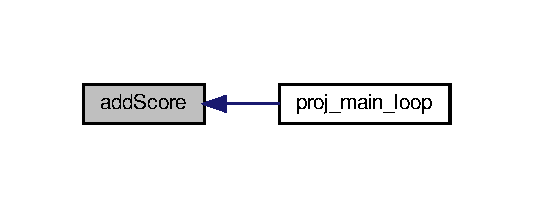
\includegraphics[width=256pt]{group__Game_ga3f24f1f331ba8708f4661eec7872b914_icgraph}
\end{center}
\end{figure}
\mbox{\Hypertarget{group__Game_gad082b8fe4e94ee090f0c6c9d11b4d565}\label{group__Game_gad082b8fe4e94ee090f0c6c9d11b4d565}} 
\index{Game@{Game}!game\+\_\+exit@{game\+\_\+exit}}
\index{game\+\_\+exit@{game\+\_\+exit}!Game@{Game}}
\subsubsection{\texorpdfstring{game\+\_\+exit()}{game\_exit()}}
{\footnotesize\ttfamily void game\+\_\+exit (\begin{DoxyParamCaption}{ }\end{DoxyParamCaption})}



Dealocates memory allocated for platform vector. 

Here is the caller graph for this function\+:\nopagebreak
\begin{figure}[H]
\begin{center}
\leavevmode
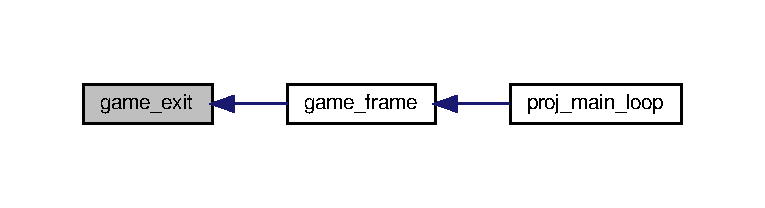
\includegraphics[width=350pt]{group__Game_gad082b8fe4e94ee090f0c6c9d11b4d565_icgraph}
\end{center}
\end{figure}
\mbox{\Hypertarget{group__Game_gad1af7212c4703893c625ad5a5e9107e0}\label{group__Game_gad1af7212c4703893c625ad5a5e9107e0}} 
\index{Game@{Game}!game\+\_\+frame@{game\+\_\+frame}}
\index{game\+\_\+frame@{game\+\_\+frame}!Game@{Game}}
\subsubsection{\texorpdfstring{game\+\_\+frame()}{game\_frame()}}
{\footnotesize\ttfamily void game\+\_\+frame (\begin{DoxyParamCaption}{ }\end{DoxyParamCaption})}



Called once per frame in game screen, manages moviment, colision, actions. 

Here is the call graph for this function\+:\nopagebreak
\begin{figure}[H]
\begin{center}
\leavevmode
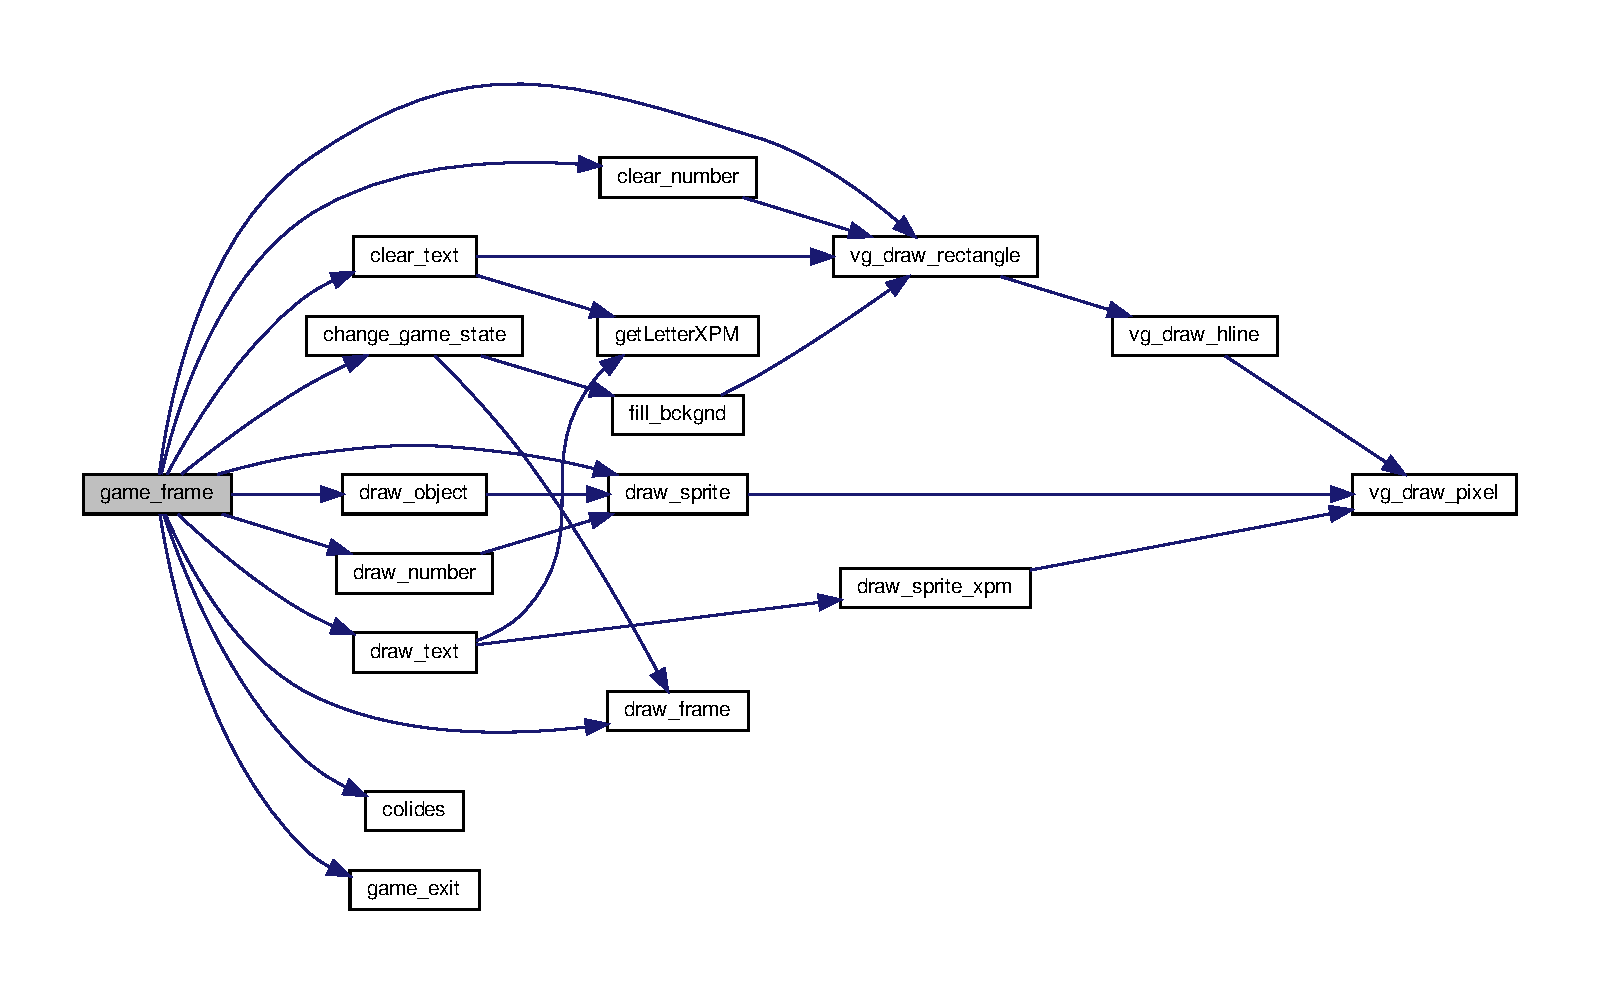
\includegraphics[width=350pt]{group__Game_gad1af7212c4703893c625ad5a5e9107e0_cgraph}
\end{center}
\end{figure}
Here is the caller graph for this function\+:\nopagebreak
\begin{figure}[H]
\begin{center}
\leavevmode
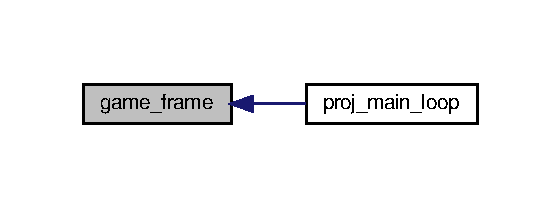
\includegraphics[width=269pt]{group__Game_gad1af7212c4703893c625ad5a5e9107e0_icgraph}
\end{center}
\end{figure}
\mbox{\Hypertarget{group__Game_ga5f5ccbe5abfdef24c8378dc3cf32ffb3}\label{group__Game_ga5f5ccbe5abfdef24c8378dc3cf32ffb3}} 
\index{Game@{Game}!game\+\_\+init@{game\+\_\+init}}
\index{game\+\_\+init@{game\+\_\+init}!Game@{Game}}
\subsubsection{\texorpdfstring{game\+\_\+init()}{game\_init()}}
{\footnotesize\ttfamily void game\+\_\+init (\begin{DoxyParamCaption}{ }\end{DoxyParamCaption})}



Initializes game variables. 

Here is the call graph for this function\+:\nopagebreak
\begin{figure}[H]
\begin{center}
\leavevmode
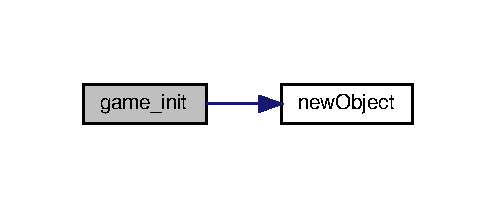
\includegraphics[width=238pt]{group__Game_ga5f5ccbe5abfdef24c8378dc3cf32ffb3_cgraph}
\end{center}
\end{figure}
Here is the caller graph for this function\+:\nopagebreak
\begin{figure}[H]
\begin{center}
\leavevmode
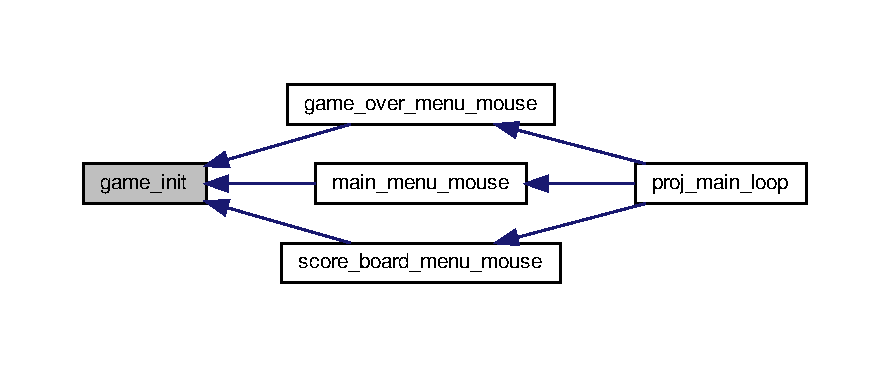
\includegraphics[width=350pt]{group__Game_ga5f5ccbe5abfdef24c8378dc3cf32ffb3_icgraph}
\end{center}
\end{figure}
\mbox{\Hypertarget{group__Game_ga51812b928d0d9e7b80bc06c044e7f5ce}\label{group__Game_ga51812b928d0d9e7b80bc06c044e7f5ce}} 
\index{Game@{Game}!game\+\_\+keyboard@{game\+\_\+keyboard}}
\index{game\+\_\+keyboard@{game\+\_\+keyboard}!Game@{Game}}
\subsubsection{\texorpdfstring{game\+\_\+keyboard()}{game\_keyboard()}}
{\footnotesize\ttfamily void game\+\_\+keyboard (\begin{DoxyParamCaption}\item[{uint8\+\_\+t}]{data }\end{DoxyParamCaption})}



Called once per keyboard interupt, manages pause and exit. 

Here is the call graph for this function\+:\nopagebreak
\begin{figure}[H]
\begin{center}
\leavevmode
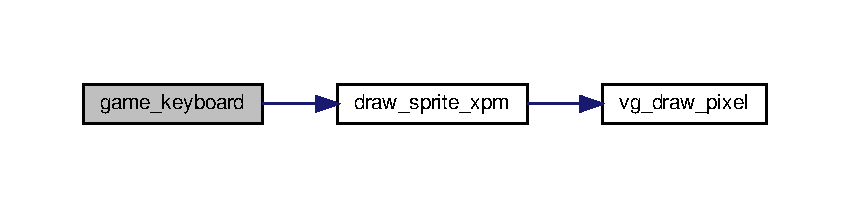
\includegraphics[width=350pt]{group__Game_ga51812b928d0d9e7b80bc06c044e7f5ce_cgraph}
\end{center}
\end{figure}
Here is the caller graph for this function\+:\nopagebreak
\begin{figure}[H]
\begin{center}
\leavevmode
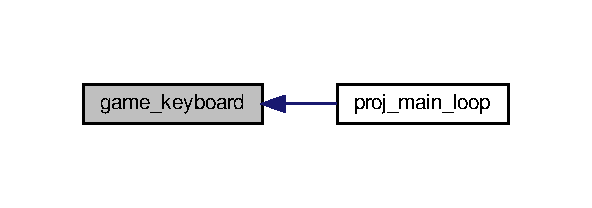
\includegraphics[width=284pt]{group__Game_ga51812b928d0d9e7b80bc06c044e7f5ce_icgraph}
\end{center}
\end{figure}
\mbox{\Hypertarget{group__Game_ga096eca75e6305cefa8171bda34e5ae42}\label{group__Game_ga096eca75e6305cefa8171bda34e5ae42}} 
\index{Game@{Game}!game\+\_\+mouse@{game\+\_\+mouse}}
\index{game\+\_\+mouse@{game\+\_\+mouse}!Game@{Game}}
\subsubsection{\texorpdfstring{game\+\_\+mouse()}{game\_mouse()}}
{\footnotesize\ttfamily void game\+\_\+mouse (\begin{DoxyParamCaption}\item[{struct packet}]{pckt }\end{DoxyParamCaption})}



Called once per mouse interupt, adds player position to mouse delta. 

Here is the caller graph for this function\+:\nopagebreak
\begin{figure}[H]
\begin{center}
\leavevmode
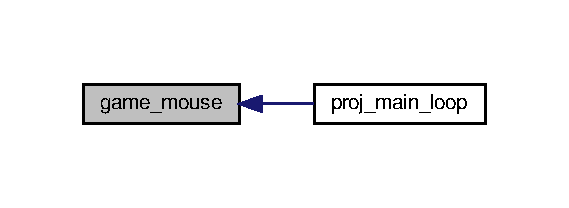
\includegraphics[width=273pt]{group__Game_ga096eca75e6305cefa8171bda34e5ae42_icgraph}
\end{center}
\end{figure}


\subsection{Variable Documentation}
\mbox{\Hypertarget{group__Game_gab3a9c86761412cb0f30bbd761491e683}\label{group__Game_gab3a9c86761412cb0f30bbd761491e683}} 
\index{Game@{Game}!acel@{acel}}
\index{acel@{acel}!Game@{Game}}
\subsubsection{\texorpdfstring{acel}{acel}}
{\footnotesize\ttfamily float acel = 1}

\mbox{\Hypertarget{group__Game_gab29a895e902e0b5c3ab2064a27af5a2d}\label{group__Game_gab29a895e902e0b5c3ab2064a27af5a2d}} 
\index{Game@{Game}!alien@{alien}}
\index{alien@{alien}!Game@{Game}}
\subsubsection{\texorpdfstring{alien}{alien}}
{\footnotesize\ttfamily \hyperlink{structObject}{Object} alien}



Player object. 

\mbox{\Hypertarget{group__Game_ga69acbc91c439d0d9f047cbe70ade84cc}\label{group__Game_ga69acbc91c439d0d9f047cbe70ade84cc}} 
\index{Game@{Game}!alien\+\_\+sprite@{alien\+\_\+sprite}}
\index{alien\+\_\+sprite@{alien\+\_\+sprite}!Game@{Game}}
\subsubsection{\texorpdfstring{alien\+\_\+sprite}{alien\_sprite}}
{\footnotesize\ttfamily xpm\+\_\+image\+\_\+t alien\+\_\+sprite}



Alien player sprite. 

\mbox{\Hypertarget{group__Game_ga5b34aa944fc2c29ad1b5e7ca7fb44449}\label{group__Game_ga5b34aa944fc2c29ad1b5e7ca7fb44449}} 
\index{Game@{Game}!asteroid\+\_\+acel@{asteroid\+\_\+acel}}
\index{asteroid\+\_\+acel@{asteroid\+\_\+acel}!Game@{Game}}
\subsubsection{\texorpdfstring{asteroid\+\_\+acel}{asteroid\_acel}}
{\footnotesize\ttfamily float asteroid\+\_\+acel = 0.\+001}



Platform aceleration. 

\mbox{\Hypertarget{group__Game_ga45f80f61d0103ffc208c2d0493380fb2}\label{group__Game_ga45f80f61d0103ffc208c2d0493380fb2}} 
\index{Game@{Game}!asteroid\+\_\+sprite@{asteroid\+\_\+sprite}}
\index{asteroid\+\_\+sprite@{asteroid\+\_\+sprite}!Game@{Game}}
\subsubsection{\texorpdfstring{asteroid\+\_\+sprite}{asteroid\_sprite}}
{\footnotesize\ttfamily xpm\+\_\+image\+\_\+t asteroid\+\_\+sprite}



Asteroid sprite. 

\mbox{\Hypertarget{group__Game_gaae54be6a12a3487f02901b15ab46a37b}\label{group__Game_gaae54be6a12a3487f02901b15ab46a37b}} 
\index{Game@{Game}!asteroid\+\_\+vel@{asteroid\+\_\+vel}}
\index{asteroid\+\_\+vel@{asteroid\+\_\+vel}!Game@{Game}}
\subsubsection{\texorpdfstring{asteroid\+\_\+vel}{asteroid\_vel}}
{\footnotesize\ttfamily float asteroid\+\_\+vel}



Platform y velocity. 

\mbox{\Hypertarget{group__Game_gae4c148b0e7f64e113a8ef493e7707429}\label{group__Game_gae4c148b0e7f64e113a8ef493e7707429}} 
\index{Game@{Game}!asteroids@{asteroids}}
\index{asteroids@{asteroids}!Game@{Game}}
\subsubsection{\texorpdfstring{asteroids}{asteroids}}
{\footnotesize\ttfamily \hyperlink{structObject}{Object}$\ast$ asteroids}



Platform vector. 

\mbox{\Hypertarget{group__Game_gad7f76af8922cce0f1ae4e8c9ed2346bd}\label{group__Game_gad7f76af8922cce0f1ae4e8c9ed2346bd}} 
\index{Game@{Game}!asteroids\+\_\+size@{asteroids\+\_\+size}}
\index{asteroids\+\_\+size@{asteroids\+\_\+size}!Game@{Game}}
\subsubsection{\texorpdfstring{asteroids\+\_\+size}{asteroids\_size}}
{\footnotesize\ttfamily int asteroids\+\_\+size = 10}



Number of platforms in screen. 

\mbox{\Hypertarget{group__Game_ga5a4cfb92e48a82e5d50c87e4bc632970}\label{group__Game_ga5a4cfb92e48a82e5d50c87e4bc632970}} 
\index{Game@{Game}!background\+\_\+sprite@{background\+\_\+sprite}}
\index{background\+\_\+sprite@{background\+\_\+sprite}!Game@{Game}}
\subsubsection{\texorpdfstring{background\+\_\+sprite}{background\_sprite}}
{\footnotesize\ttfamily xpm\+\_\+image\+\_\+t background\+\_\+sprite}



Background sprite. 

\mbox{\Hypertarget{group__Game_ga223eb1bebc2dce2b95cb54c56c82b040}\label{group__Game_ga223eb1bebc2dce2b95cb54c56c82b040}} 
\index{Game@{Game}!bounce\+\_\+vel@{bounce\+\_\+vel}}
\index{bounce\+\_\+vel@{bounce\+\_\+vel}!Game@{Game}}
\subsubsection{\texorpdfstring{bounce\+\_\+vel}{bounce\_vel}}
{\footnotesize\ttfamily float bounce\+\_\+vel = -\/20}



Velocity the player bounces back from a platform. 

\mbox{\Hypertarget{group__Game_ga06a70f098733d826cb9d8e81e7104983}\label{group__Game_ga06a70f098733d826cb9d8e81e7104983}} 
\index{Game@{Game}!broken\+\_\+asteroid\+\_\+sprite@{broken\+\_\+asteroid\+\_\+sprite}}
\index{broken\+\_\+asteroid\+\_\+sprite@{broken\+\_\+asteroid\+\_\+sprite}!Game@{Game}}
\subsubsection{\texorpdfstring{broken\+\_\+asteroid\+\_\+sprite}{broken\_asteroid\_sprite}}
{\footnotesize\ttfamily xpm\+\_\+image\+\_\+t broken\+\_\+asteroid\+\_\+sprite}



Broken asteroid sprite. 

\mbox{\Hypertarget{group__Game_ga38caf7c28534bcd60ff95faf7fcae2d7}\label{group__Game_ga38caf7c28534bcd60ff95faf7fcae2d7}} 
\index{Game@{Game}!game\+\_\+state@{game\+\_\+state}}
\index{game\+\_\+state@{game\+\_\+state}!Game@{Game}}
\subsubsection{\texorpdfstring{game\+\_\+state}{game\_state}}
{\footnotesize\ttfamily enum \hyperlink{group__utils_gad0ed1832dd134806ad335cdcc1a59ad2}{game\+\_\+state} \hyperlink{group__utils_gad0ed1832dd134806ad335cdcc1a59ad2}{game\+\_\+state}}



Current game state. 

\mbox{\Hypertarget{group__Game_gafef635ed3c73fc60d8faf6dd610c4298}\label{group__Game_gafef635ed3c73fc60d8faf6dd610c4298}} 
\index{Game@{Game}!ox@{ox}}
\index{ox@{ox}!Game@{Game}}
\subsubsection{\texorpdfstring{ox}{ox}}
{\footnotesize\ttfamily int ox = 0}



Value of the player x in the last frame, to erease the image. 

\mbox{\Hypertarget{group__Game_ga1656129c4a4fd8809254194f08f0ac70}\label{group__Game_ga1656129c4a4fd8809254194f08f0ac70}} 
\index{Game@{Game}!paused@{paused}}
\index{paused@{paused}!Game@{Game}}
\subsubsection{\texorpdfstring{paused}{paused}}
{\footnotesize\ttfamily bool paused = false}



If the game is paused or not. 

\mbox{\Hypertarget{group__Game_gaef160b7437d94056f1dc59646cd5b87d}\label{group__Game_gaef160b7437d94056f1dc59646cd5b87d}} 
\index{Game@{Game}!score@{score}}
\index{score@{score}!Game@{Game}}
\subsubsection{\texorpdfstring{score}{score}}
{\footnotesize\ttfamily int score}



Player score. 

\mbox{\Hypertarget{group__Game_gafc29fb7fadd39a1bc2e3c52532248689}\label{group__Game_gafc29fb7fadd39a1bc2e3c52532248689}} 
\index{Game@{Game}!vel@{vel}}
\index{vel@{vel}!Game@{Game}}
\subsubsection{\texorpdfstring{vel}{vel}}
{\footnotesize\ttfamily float vel}



Player y velocity. 


\hypertarget{group__Game-Over-Menu}{}\section{Game-\/\+Over-\/\+Menu}
\label{group__Game-Over-Menu}\index{Game-\/\+Over-\/\+Menu@{Game-\/\+Over-\/\+Menu}}
\subsection*{Functions}
\begin{DoxyCompactItemize}
\item 
void \hyperlink{group__Game-Over-Menu_ga8105461ec4f2f3dc83bf6b821b353144}{game\+\_\+over\+\_\+menu\+\_\+frame} ()
\begin{DoxyCompactList}\small\item\em Called once per frama, draws the menu and mouse cursor. \end{DoxyCompactList}\item 
void \hyperlink{group__Game-Over-Menu_gaacffded003ea0e055b93b3cf2bf26293}{update\+\_\+score\+\_\+board} ()
\begin{DoxyCompactList}\small\item\em Adds the current score the the top 10 scores array and file. \end{DoxyCompactList}\item 
void \hyperlink{group__Game-Over-Menu_ga8a878da05a37cf4c3e82b28282dc5c47}{game\+\_\+over\+\_\+menu\+\_\+keyboard} (uint8\+\_\+t \hyperlink{group__Proj_ga325819a8e492ac69542e8b31705af6e9}{data})
\begin{DoxyCompactList}\small\item\em Called once per mouse interupt, manages exit and name insertion. \end{DoxyCompactList}\item 
void \hyperlink{group__Game-Over-Menu_gae4cc6accba6062a3b5855bfc3826b215}{game\+\_\+over\+\_\+menu\+\_\+mouse} (struct packet pckt)
\begin{DoxyCompactList}\small\item\em Called once per mouse interupt, manages mouse cursor and click. \end{DoxyCompactList}\end{DoxyCompactItemize}
\subsection*{Variables}
\begin{DoxyCompactItemize}
\item 
enum \hyperlink{group__utils_gad0ed1832dd134806ad335cdcc1a59ad2}{game\+\_\+state} \hyperlink{group__Game-Over-Menu_ga38caf7c28534bcd60ff95faf7fcae2d7}{game\+\_\+state}
\begin{DoxyCompactList}\small\item\em Current game state. \end{DoxyCompactList}\item 
bool \hyperlink{group__Game-Over-Menu_ga11932993f5f2c243a9c6e09519cf1b73}{drawn\+\_\+} = false
\begin{DoxyCompactList}\small\item\em If the program just entered this screen is false, then it turns true. \end{DoxyCompactList}\item 
int \hyperlink{group__Game-Over-Menu_gaef160b7437d94056f1dc59646cd5b87d}{score}
\begin{DoxyCompactList}\small\item\em Player score. \end{DoxyCompactList}\item 
char \hyperlink{group__Game-Over-Menu_gae3b2d5dad8a568a12752edcea2435e50}{str} \mbox{[}99\mbox{]}
\begin{DoxyCompactList}\small\item\em Will record the user input for the score board. \end{DoxyCompactList}\item 
int \hyperlink{group__Game-Over-Menu_ga439227feff9d7f55384e8780cfc2eb82}{size} = 0
\begin{DoxyCompactList}\small\item\em The size of the user input. \end{DoxyCompactList}\item 
int \hyperlink{group__Game-Over-Menu_ga6c59af730728bf5260ef828aea2eebee}{mouse\+\_\+x}
\begin{DoxyCompactList}\small\item\em Mouse x position. \end{DoxyCompactList}\item 
int \hyperlink{group__Game-Over-Menu_gab21653e455bbca86826aa5f628a5fdb2}{mouse\+\_\+y}
\begin{DoxyCompactList}\small\item\em Mouse y position. \end{DoxyCompactList}\item 
int \hyperlink{group__Game-Over-Menu_gad7f272c01893c7161961744eb23516d0}{o\+\_\+mouse\+\_\+x}
\begin{DoxyCompactList}\small\item\em Mouse x position in last frame. \end{DoxyCompactList}\item 
int \hyperlink{group__Game-Over-Menu_ga7c7344b212ca479c18185090a37e0d29}{o\+\_\+mouse\+\_\+y}
\begin{DoxyCompactList}\small\item\em Mouse y position in last frame. \end{DoxyCompactList}\item 
xpm\+\_\+image\+\_\+t \hyperlink{group__Game-Over-Menu_ga1713b7f6ecba05ea9e8281f216eb8818}{mouse\+\_\+sprite}
\begin{DoxyCompactList}\small\item\em Mouse cursor sprite. \end{DoxyCompactList}\item 
xpm\+\_\+image\+\_\+t \hyperlink{group__Game-Over-Menu_ga151ed16274d40549e8aa6715aa4c715a}{exit\+\_\+sprite}
\begin{DoxyCompactList}\small\item\em Exit button sprite. \end{DoxyCompactList}\item 
xpm\+\_\+image\+\_\+t \hyperlink{group__Game-Over-Menu_ga75a1070484069c0a4b134cb82e89285f}{game\+\_\+over\+\_\+sprite}
\begin{DoxyCompactList}\small\item\em Game over text sprite. \end{DoxyCompactList}\item 
xpm\+\_\+image\+\_\+t \hyperlink{group__Game-Over-Menu_ga9c8097218050947104e9eff7ea72ee2a}{score\+\_\+sprite}
\begin{DoxyCompactList}\small\item\em Score text sprite. \end{DoxyCompactList}\item 
xpm\+\_\+image\+\_\+t \hyperlink{group__Game-Over-Menu_gaa41380dca9e42a7214c4383a057eb1b5}{try\+\_\+again\+\_\+sprite}
\begin{DoxyCompactList}\small\item\em try again button sprite \end{DoxyCompactList}\item 
xpm\+\_\+image\+\_\+t \hyperlink{group__Game-Over-Menu_ga4e9f74a7ebd652ff9289c657ccbcbad2}{score\+\_\+board\+\_\+sprite}
\begin{DoxyCompactList}\small\item\em score board button sprite \end{DoxyCompactList}\item 
int \hyperlink{group__Game-Over-Menu_ga10efae42dd260dcc2c52eb07d71da687}{highscores} \mbox{[}\hyperlink{group__utils_ga85e9c9dc96b1373ebdb408da38eb5367}{S\+C\+O\+R\+E\+\_\+\+B\+O\+A\+R\+D\+\_\+\+S\+I\+ZE}\mbox{]}
\begin{DoxyCompactList}\small\item\em Top scores array. \end{DoxyCompactList}\item 
char \hyperlink{group__Game-Over-Menu_ga286661e657548eadd26d0d129c981ea2}{names} \mbox{[}\hyperlink{group__utils_ga85e9c9dc96b1373ebdb408da38eb5367}{S\+C\+O\+R\+E\+\_\+\+B\+O\+A\+R\+D\+\_\+\+S\+I\+ZE}\mbox{]}\mbox{[}255\mbox{]}
\begin{DoxyCompactList}\small\item\em Top score player name array. \end{DoxyCompactList}\end{DoxyCompactItemize}


\subsection{Detailed Description}
Contais tha code for the game over screen 

\subsection{Function Documentation}
\mbox{\Hypertarget{group__Game-Over-Menu_ga8105461ec4f2f3dc83bf6b821b353144}\label{group__Game-Over-Menu_ga8105461ec4f2f3dc83bf6b821b353144}} 
\index{Game-\/\+Over-\/\+Menu@{Game-\/\+Over-\/\+Menu}!game\+\_\+over\+\_\+menu\+\_\+frame@{game\+\_\+over\+\_\+menu\+\_\+frame}}
\index{game\+\_\+over\+\_\+menu\+\_\+frame@{game\+\_\+over\+\_\+menu\+\_\+frame}!Game-\/\+Over-\/\+Menu@{Game-\/\+Over-\/\+Menu}}
\subsubsection{\texorpdfstring{game\+\_\+over\+\_\+menu\+\_\+frame()}{game\_over\_menu\_frame()}}
{\footnotesize\ttfamily void game\+\_\+over\+\_\+menu\+\_\+frame (\begin{DoxyParamCaption}{ }\end{DoxyParamCaption})}



Called once per frama, draws the menu and mouse cursor. 

Here is the call graph for this function\+:\nopagebreak
\begin{figure}[H]
\begin{center}
\leavevmode
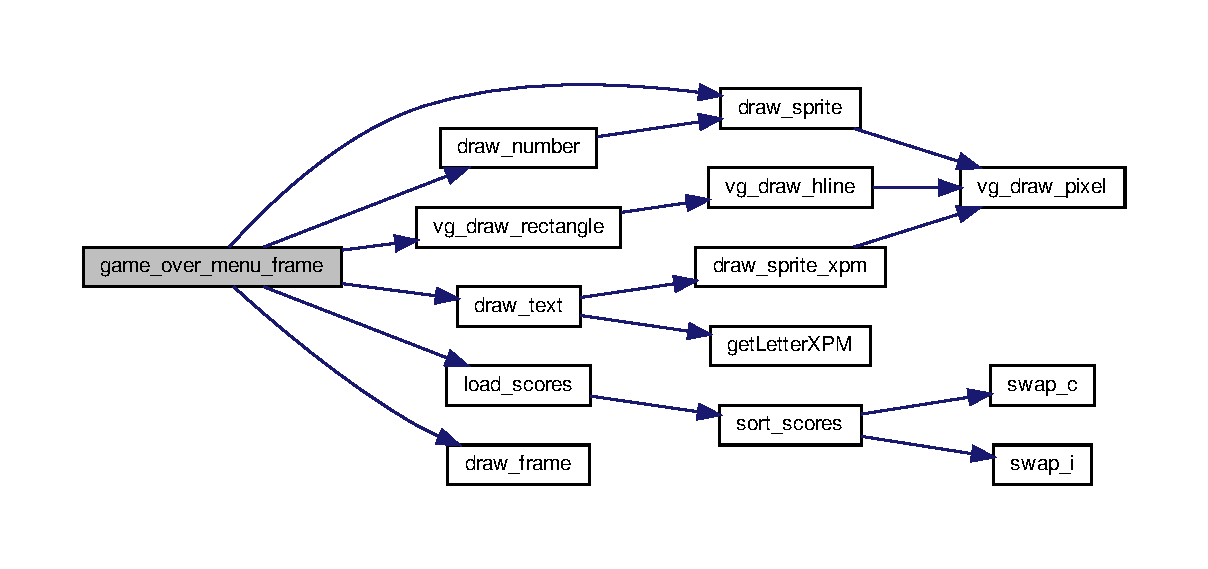
\includegraphics[width=350pt]{group__Game-Over-Menu_ga8105461ec4f2f3dc83bf6b821b353144_cgraph}
\end{center}
\end{figure}
Here is the caller graph for this function\+:\nopagebreak
\begin{figure}[H]
\begin{center}
\leavevmode
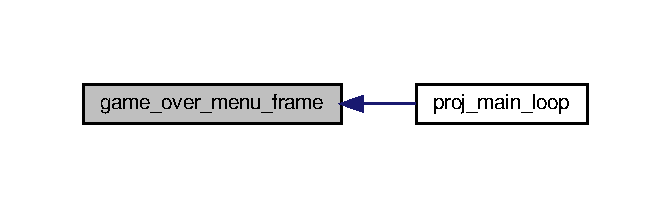
\includegraphics[width=322pt]{group__Game-Over-Menu_ga8105461ec4f2f3dc83bf6b821b353144_icgraph}
\end{center}
\end{figure}
\mbox{\Hypertarget{group__Game-Over-Menu_ga8a878da05a37cf4c3e82b28282dc5c47}\label{group__Game-Over-Menu_ga8a878da05a37cf4c3e82b28282dc5c47}} 
\index{Game-\/\+Over-\/\+Menu@{Game-\/\+Over-\/\+Menu}!game\+\_\+over\+\_\+menu\+\_\+keyboard@{game\+\_\+over\+\_\+menu\+\_\+keyboard}}
\index{game\+\_\+over\+\_\+menu\+\_\+keyboard@{game\+\_\+over\+\_\+menu\+\_\+keyboard}!Game-\/\+Over-\/\+Menu@{Game-\/\+Over-\/\+Menu}}
\subsubsection{\texorpdfstring{game\+\_\+over\+\_\+menu\+\_\+keyboard()}{game\_over\_menu\_keyboard()}}
{\footnotesize\ttfamily void game\+\_\+over\+\_\+menu\+\_\+keyboard (\begin{DoxyParamCaption}\item[{uint8\+\_\+t}]{data }\end{DoxyParamCaption})}



Called once per mouse interupt, manages exit and name insertion. 

Here is the call graph for this function\+:
\nopagebreak
\begin{figure}[H]
\begin{center}
\leavevmode
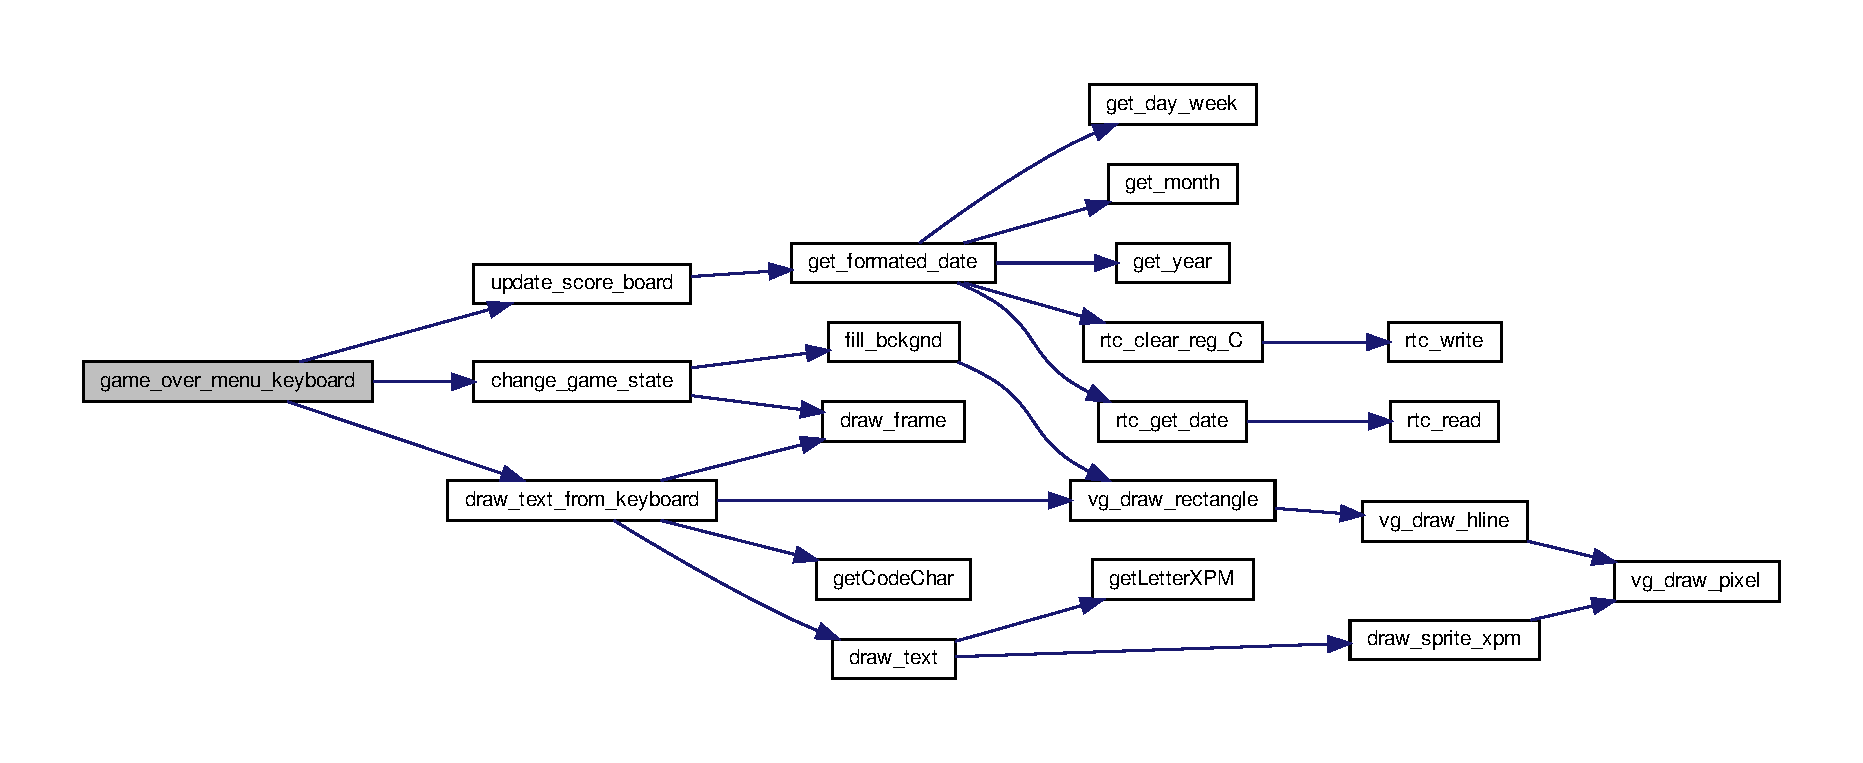
\includegraphics[width=350pt]{group__Game-Over-Menu_ga8a878da05a37cf4c3e82b28282dc5c47_cgraph}
\end{center}
\end{figure}
Here is the caller graph for this function\+:
\nopagebreak
\begin{figure}[H]
\begin{center}
\leavevmode
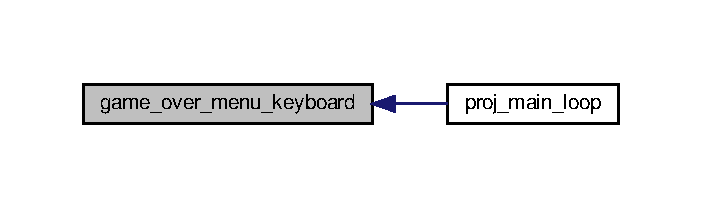
\includegraphics[width=337pt]{group__Game-Over-Menu_ga8a878da05a37cf4c3e82b28282dc5c47_icgraph}
\end{center}
\end{figure}
\mbox{\Hypertarget{group__Game-Over-Menu_gae4cc6accba6062a3b5855bfc3826b215}\label{group__Game-Over-Menu_gae4cc6accba6062a3b5855bfc3826b215}} 
\index{Game-\/\+Over-\/\+Menu@{Game-\/\+Over-\/\+Menu}!game\+\_\+over\+\_\+menu\+\_\+mouse@{game\+\_\+over\+\_\+menu\+\_\+mouse}}
\index{game\+\_\+over\+\_\+menu\+\_\+mouse@{game\+\_\+over\+\_\+menu\+\_\+mouse}!Game-\/\+Over-\/\+Menu@{Game-\/\+Over-\/\+Menu}}
\subsubsection{\texorpdfstring{game\+\_\+over\+\_\+menu\+\_\+mouse()}{game\_over\_menu\_mouse()}}
{\footnotesize\ttfamily void game\+\_\+over\+\_\+menu\+\_\+mouse (\begin{DoxyParamCaption}\item[{struct packet}]{pckt }\end{DoxyParamCaption})}



Called once per mouse interupt, manages mouse cursor and click. 

Here is the call graph for this function\+:
\nopagebreak
\begin{figure}[H]
\begin{center}
\leavevmode
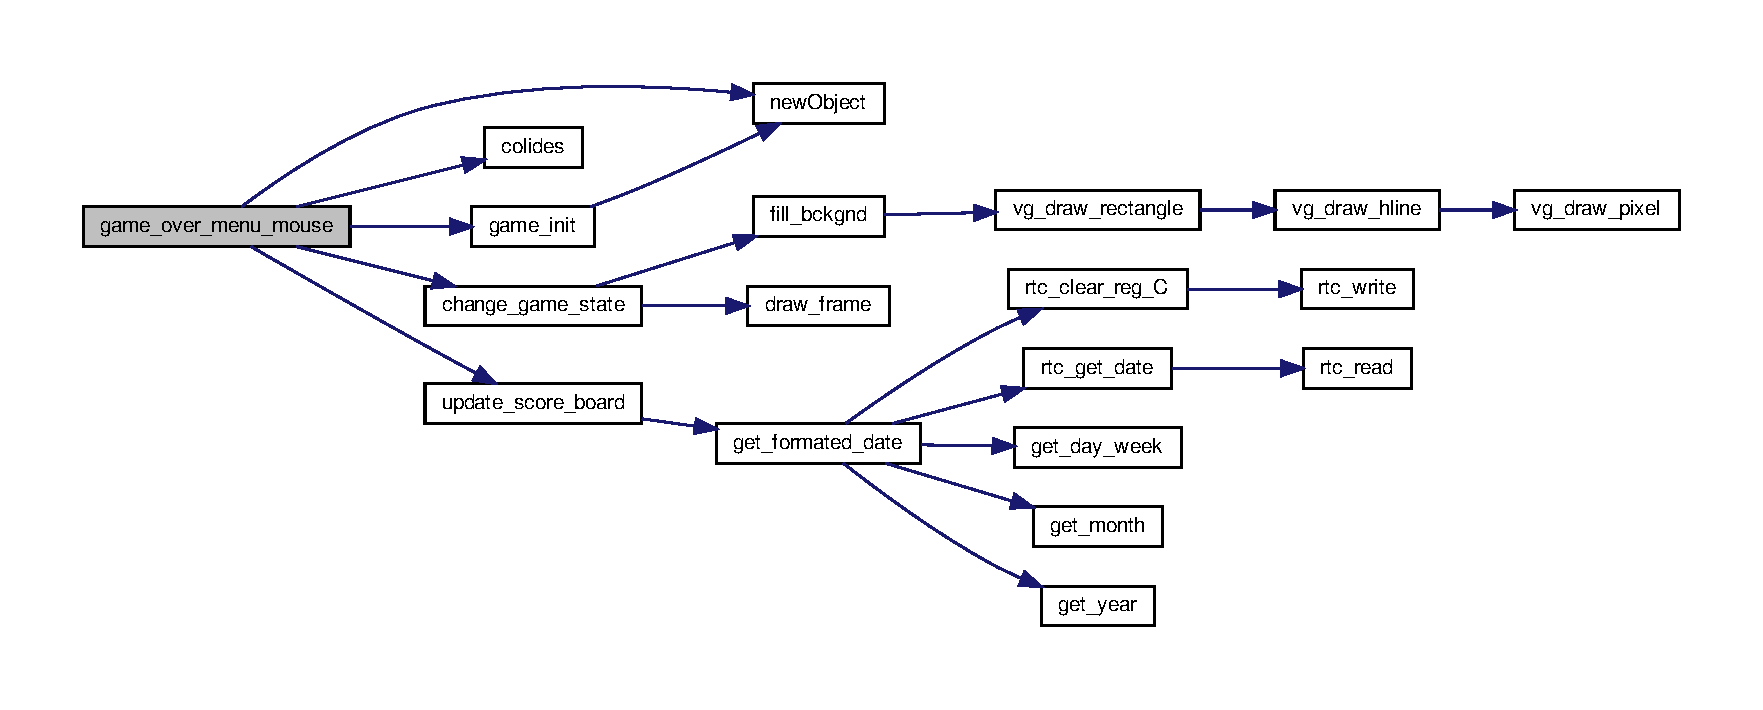
\includegraphics[width=350pt]{group__Game-Over-Menu_gae4cc6accba6062a3b5855bfc3826b215_cgraph}
\end{center}
\end{figure}
Here is the caller graph for this function\+:
\nopagebreak
\begin{figure}[H]
\begin{center}
\leavevmode
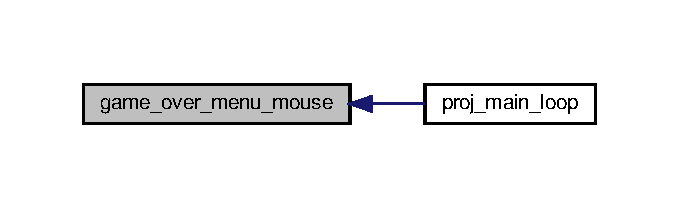
\includegraphics[width=326pt]{group__Game-Over-Menu_gae4cc6accba6062a3b5855bfc3826b215_icgraph}
\end{center}
\end{figure}
\mbox{\Hypertarget{group__Game-Over-Menu_gaacffded003ea0e055b93b3cf2bf26293}\label{group__Game-Over-Menu_gaacffded003ea0e055b93b3cf2bf26293}} 
\index{Game-\/\+Over-\/\+Menu@{Game-\/\+Over-\/\+Menu}!update\+\_\+score\+\_\+board@{update\+\_\+score\+\_\+board}}
\index{update\+\_\+score\+\_\+board@{update\+\_\+score\+\_\+board}!Game-\/\+Over-\/\+Menu@{Game-\/\+Over-\/\+Menu}}
\subsubsection{\texorpdfstring{update\+\_\+score\+\_\+board()}{update\_score\_board()}}
{\footnotesize\ttfamily void update\+\_\+score\+\_\+board (\begin{DoxyParamCaption}{ }\end{DoxyParamCaption})}



Adds the current score the the top 10 scores array and file. 

Here is the call graph for this function\+:
\nopagebreak
\begin{figure}[H]
\begin{center}
\leavevmode
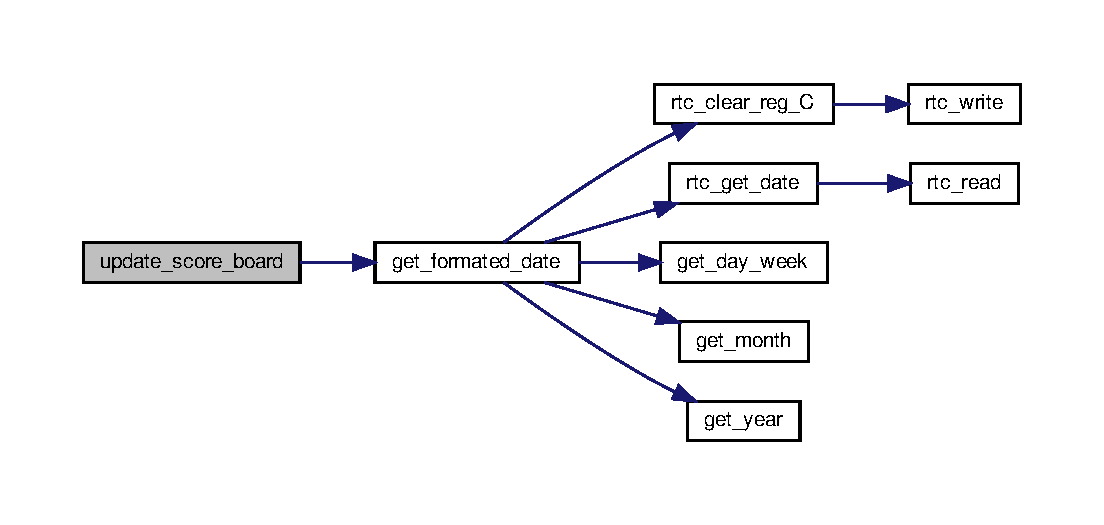
\includegraphics[width=350pt]{group__Game-Over-Menu_gaacffded003ea0e055b93b3cf2bf26293_cgraph}
\end{center}
\end{figure}
Here is the caller graph for this function\+:
\nopagebreak
\begin{figure}[H]
\begin{center}
\leavevmode
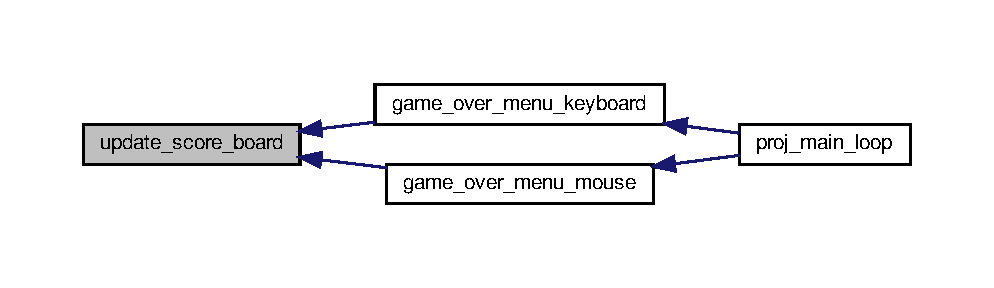
\includegraphics[width=350pt]{group__Game-Over-Menu_gaacffded003ea0e055b93b3cf2bf26293_icgraph}
\end{center}
\end{figure}


\subsection{Variable Documentation}
\mbox{\Hypertarget{group__Game-Over-Menu_ga11932993f5f2c243a9c6e09519cf1b73}\label{group__Game-Over-Menu_ga11932993f5f2c243a9c6e09519cf1b73}} 
\index{Game-\/\+Over-\/\+Menu@{Game-\/\+Over-\/\+Menu}!drawn\+\_\+@{drawn\+\_\+}}
\index{drawn\+\_\+@{drawn\+\_\+}!Game-\/\+Over-\/\+Menu@{Game-\/\+Over-\/\+Menu}}
\subsubsection{\texorpdfstring{drawn\+\_\+}{drawn\_}}
{\footnotesize\ttfamily bool drawn\+\_\+ = false}



If the program just entered this screen is false, then it turns true. 

\mbox{\Hypertarget{group__Game-Over-Menu_ga151ed16274d40549e8aa6715aa4c715a}\label{group__Game-Over-Menu_ga151ed16274d40549e8aa6715aa4c715a}} 
\index{Game-\/\+Over-\/\+Menu@{Game-\/\+Over-\/\+Menu}!exit\+\_\+sprite@{exit\+\_\+sprite}}
\index{exit\+\_\+sprite@{exit\+\_\+sprite}!Game-\/\+Over-\/\+Menu@{Game-\/\+Over-\/\+Menu}}
\subsubsection{\texorpdfstring{exit\+\_\+sprite}{exit\_sprite}}
{\footnotesize\ttfamily xpm\+\_\+image\+\_\+t exit\+\_\+sprite}



Exit button sprite. 

\mbox{\Hypertarget{group__Game-Over-Menu_ga75a1070484069c0a4b134cb82e89285f}\label{group__Game-Over-Menu_ga75a1070484069c0a4b134cb82e89285f}} 
\index{Game-\/\+Over-\/\+Menu@{Game-\/\+Over-\/\+Menu}!game\+\_\+over\+\_\+sprite@{game\+\_\+over\+\_\+sprite}}
\index{game\+\_\+over\+\_\+sprite@{game\+\_\+over\+\_\+sprite}!Game-\/\+Over-\/\+Menu@{Game-\/\+Over-\/\+Menu}}
\subsubsection{\texorpdfstring{game\+\_\+over\+\_\+sprite}{game\_over\_sprite}}
{\footnotesize\ttfamily xpm\+\_\+image\+\_\+t game\+\_\+over\+\_\+sprite}



Game over text sprite. 

\mbox{\Hypertarget{group__Game-Over-Menu_ga38caf7c28534bcd60ff95faf7fcae2d7}\label{group__Game-Over-Menu_ga38caf7c28534bcd60ff95faf7fcae2d7}} 
\index{Game-\/\+Over-\/\+Menu@{Game-\/\+Over-\/\+Menu}!game\+\_\+state@{game\+\_\+state}}
\index{game\+\_\+state@{game\+\_\+state}!Game-\/\+Over-\/\+Menu@{Game-\/\+Over-\/\+Menu}}
\subsubsection{\texorpdfstring{game\+\_\+state}{game\_state}}
{\footnotesize\ttfamily enum \hyperlink{group__utils_gad0ed1832dd134806ad335cdcc1a59ad2}{game\+\_\+state} \hyperlink{group__utils_gad0ed1832dd134806ad335cdcc1a59ad2}{game\+\_\+state}}



Current game state. 

\mbox{\Hypertarget{group__Game-Over-Menu_ga10efae42dd260dcc2c52eb07d71da687}\label{group__Game-Over-Menu_ga10efae42dd260dcc2c52eb07d71da687}} 
\index{Game-\/\+Over-\/\+Menu@{Game-\/\+Over-\/\+Menu}!highscores@{highscores}}
\index{highscores@{highscores}!Game-\/\+Over-\/\+Menu@{Game-\/\+Over-\/\+Menu}}
\subsubsection{\texorpdfstring{highscores}{highscores}}
{\footnotesize\ttfamily int highscores\mbox{[}\hyperlink{group__utils_ga85e9c9dc96b1373ebdb408da38eb5367}{S\+C\+O\+R\+E\+\_\+\+B\+O\+A\+R\+D\+\_\+\+S\+I\+ZE}\mbox{]}}



Top scores array. 

\mbox{\Hypertarget{group__Game-Over-Menu_ga1713b7f6ecba05ea9e8281f216eb8818}\label{group__Game-Over-Menu_ga1713b7f6ecba05ea9e8281f216eb8818}} 
\index{Game-\/\+Over-\/\+Menu@{Game-\/\+Over-\/\+Menu}!mouse\+\_\+sprite@{mouse\+\_\+sprite}}
\index{mouse\+\_\+sprite@{mouse\+\_\+sprite}!Game-\/\+Over-\/\+Menu@{Game-\/\+Over-\/\+Menu}}
\subsubsection{\texorpdfstring{mouse\+\_\+sprite}{mouse\_sprite}}
{\footnotesize\ttfamily xpm\+\_\+image\+\_\+t mouse\+\_\+sprite}



Mouse cursor sprite. 

\mbox{\Hypertarget{group__Game-Over-Menu_ga6c59af730728bf5260ef828aea2eebee}\label{group__Game-Over-Menu_ga6c59af730728bf5260ef828aea2eebee}} 
\index{Game-\/\+Over-\/\+Menu@{Game-\/\+Over-\/\+Menu}!mouse\+\_\+x@{mouse\+\_\+x}}
\index{mouse\+\_\+x@{mouse\+\_\+x}!Game-\/\+Over-\/\+Menu@{Game-\/\+Over-\/\+Menu}}
\subsubsection{\texorpdfstring{mouse\+\_\+x}{mouse\_x}}
{\footnotesize\ttfamily int mouse\+\_\+x}



Mouse x position. 

\mbox{\Hypertarget{group__Game-Over-Menu_gab21653e455bbca86826aa5f628a5fdb2}\label{group__Game-Over-Menu_gab21653e455bbca86826aa5f628a5fdb2}} 
\index{Game-\/\+Over-\/\+Menu@{Game-\/\+Over-\/\+Menu}!mouse\+\_\+y@{mouse\+\_\+y}}
\index{mouse\+\_\+y@{mouse\+\_\+y}!Game-\/\+Over-\/\+Menu@{Game-\/\+Over-\/\+Menu}}
\subsubsection{\texorpdfstring{mouse\+\_\+y}{mouse\_y}}
{\footnotesize\ttfamily int mouse\+\_\+y}



Mouse y position. 

\mbox{\Hypertarget{group__Game-Over-Menu_ga286661e657548eadd26d0d129c981ea2}\label{group__Game-Over-Menu_ga286661e657548eadd26d0d129c981ea2}} 
\index{Game-\/\+Over-\/\+Menu@{Game-\/\+Over-\/\+Menu}!names@{names}}
\index{names@{names}!Game-\/\+Over-\/\+Menu@{Game-\/\+Over-\/\+Menu}}
\subsubsection{\texorpdfstring{names}{names}}
{\footnotesize\ttfamily char names\mbox{[}\hyperlink{group__utils_ga85e9c9dc96b1373ebdb408da38eb5367}{S\+C\+O\+R\+E\+\_\+\+B\+O\+A\+R\+D\+\_\+\+S\+I\+ZE}\mbox{]}\mbox{[}255\mbox{]}}



Top score player name array. 

\mbox{\Hypertarget{group__Game-Over-Menu_gad7f272c01893c7161961744eb23516d0}\label{group__Game-Over-Menu_gad7f272c01893c7161961744eb23516d0}} 
\index{Game-\/\+Over-\/\+Menu@{Game-\/\+Over-\/\+Menu}!o\+\_\+mouse\+\_\+x@{o\+\_\+mouse\+\_\+x}}
\index{o\+\_\+mouse\+\_\+x@{o\+\_\+mouse\+\_\+x}!Game-\/\+Over-\/\+Menu@{Game-\/\+Over-\/\+Menu}}
\subsubsection{\texorpdfstring{o\+\_\+mouse\+\_\+x}{o\_mouse\_x}}
{\footnotesize\ttfamily int o\+\_\+mouse\+\_\+x}



Mouse x position in last frame. 

\mbox{\Hypertarget{group__Game-Over-Menu_ga7c7344b212ca479c18185090a37e0d29}\label{group__Game-Over-Menu_ga7c7344b212ca479c18185090a37e0d29}} 
\index{Game-\/\+Over-\/\+Menu@{Game-\/\+Over-\/\+Menu}!o\+\_\+mouse\+\_\+y@{o\+\_\+mouse\+\_\+y}}
\index{o\+\_\+mouse\+\_\+y@{o\+\_\+mouse\+\_\+y}!Game-\/\+Over-\/\+Menu@{Game-\/\+Over-\/\+Menu}}
\subsubsection{\texorpdfstring{o\+\_\+mouse\+\_\+y}{o\_mouse\_y}}
{\footnotesize\ttfamily int o\+\_\+mouse\+\_\+y}



Mouse y position in last frame. 

\mbox{\Hypertarget{group__Game-Over-Menu_gaef160b7437d94056f1dc59646cd5b87d}\label{group__Game-Over-Menu_gaef160b7437d94056f1dc59646cd5b87d}} 
\index{Game-\/\+Over-\/\+Menu@{Game-\/\+Over-\/\+Menu}!score@{score}}
\index{score@{score}!Game-\/\+Over-\/\+Menu@{Game-\/\+Over-\/\+Menu}}
\subsubsection{\texorpdfstring{score}{score}}
{\footnotesize\ttfamily int score}



Player score. 

\mbox{\Hypertarget{group__Game-Over-Menu_ga4e9f74a7ebd652ff9289c657ccbcbad2}\label{group__Game-Over-Menu_ga4e9f74a7ebd652ff9289c657ccbcbad2}} 
\index{Game-\/\+Over-\/\+Menu@{Game-\/\+Over-\/\+Menu}!score\+\_\+board\+\_\+sprite@{score\+\_\+board\+\_\+sprite}}
\index{score\+\_\+board\+\_\+sprite@{score\+\_\+board\+\_\+sprite}!Game-\/\+Over-\/\+Menu@{Game-\/\+Over-\/\+Menu}}
\subsubsection{\texorpdfstring{score\+\_\+board\+\_\+sprite}{score\_board\_sprite}}
{\footnotesize\ttfamily xpm\+\_\+image\+\_\+t score\+\_\+board\+\_\+sprite}



score board button sprite 

\mbox{\Hypertarget{group__Game-Over-Menu_ga9c8097218050947104e9eff7ea72ee2a}\label{group__Game-Over-Menu_ga9c8097218050947104e9eff7ea72ee2a}} 
\index{Game-\/\+Over-\/\+Menu@{Game-\/\+Over-\/\+Menu}!score\+\_\+sprite@{score\+\_\+sprite}}
\index{score\+\_\+sprite@{score\+\_\+sprite}!Game-\/\+Over-\/\+Menu@{Game-\/\+Over-\/\+Menu}}
\subsubsection{\texorpdfstring{score\+\_\+sprite}{score\_sprite}}
{\footnotesize\ttfamily xpm\+\_\+image\+\_\+t score\+\_\+sprite}



Score text sprite. 

\mbox{\Hypertarget{group__Game-Over-Menu_ga439227feff9d7f55384e8780cfc2eb82}\label{group__Game-Over-Menu_ga439227feff9d7f55384e8780cfc2eb82}} 
\index{Game-\/\+Over-\/\+Menu@{Game-\/\+Over-\/\+Menu}!size@{size}}
\index{size@{size}!Game-\/\+Over-\/\+Menu@{Game-\/\+Over-\/\+Menu}}
\subsubsection{\texorpdfstring{size}{size}}
{\footnotesize\ttfamily int size = 0}



The size of the user input. 

\mbox{\Hypertarget{group__Game-Over-Menu_gae3b2d5dad8a568a12752edcea2435e50}\label{group__Game-Over-Menu_gae3b2d5dad8a568a12752edcea2435e50}} 
\index{Game-\/\+Over-\/\+Menu@{Game-\/\+Over-\/\+Menu}!str@{str}}
\index{str@{str}!Game-\/\+Over-\/\+Menu@{Game-\/\+Over-\/\+Menu}}
\subsubsection{\texorpdfstring{str}{str}}
{\footnotesize\ttfamily char str\mbox{[}99\mbox{]}}



Will record the user input for the score board. 

\mbox{\Hypertarget{group__Game-Over-Menu_gaa41380dca9e42a7214c4383a057eb1b5}\label{group__Game-Over-Menu_gaa41380dca9e42a7214c4383a057eb1b5}} 
\index{Game-\/\+Over-\/\+Menu@{Game-\/\+Over-\/\+Menu}!try\+\_\+again\+\_\+sprite@{try\+\_\+again\+\_\+sprite}}
\index{try\+\_\+again\+\_\+sprite@{try\+\_\+again\+\_\+sprite}!Game-\/\+Over-\/\+Menu@{Game-\/\+Over-\/\+Menu}}
\subsubsection{\texorpdfstring{try\+\_\+again\+\_\+sprite}{try\_again\_sprite}}
{\footnotesize\ttfamily xpm\+\_\+image\+\_\+t try\+\_\+again\+\_\+sprite}



try again button sprite 


\hypertarget{group__graphics}{}\section{graphics}
\label{group__graphics}\index{graphics@{graphics}}
\subsection*{Functions}
\begin{DoxyCompactItemize}
\item 
void() \hyperlink{group__graphics_gae70314d2e6e41dae20ce327a13929401}{draw\+\_\+frame} ()
\begin{DoxyCompactList}\small\item\em Draw video buffer into video memory. \end{DoxyCompactList}\item 
void() \hyperlink{group__graphics_ga427099c53976d605666e7e2b39238bb9}{free\+\_\+buffer} ()
\begin{DoxyCompactList}\small\item\em Dealocates video buffer. \end{DoxyCompactList}\item 
int() \hyperlink{group__graphics_gac34ed31db6d6ef68b7167a0c024cac2b}{vg\+\_\+enter} (uint16\+\_\+t mode)
\begin{DoxyCompactList}\small\item\em Enters video mode in the given mode. \end{DoxyCompactList}\item 
void $\ast$() \hyperlink{group__graphics_gaa6c1ff5024cd4d15e476bce487584daa}{vg\+\_\+init} (uint16\+\_\+t mode)
\begin{DoxyCompactList}\small\item\em Initializes video grafics variables. \end{DoxyCompactList}\item 
int() \hyperlink{group__graphics_ga08c498ffeb0a3962e3b7711b57397741}{vg\+\_\+draw\+\_\+pixel} (uint16\+\_\+t x, uint16\+\_\+t y, uint32\+\_\+t color)
\begin{DoxyCompactList}\small\item\em Turns the given x,y position pixel to the given color. \end{DoxyCompactList}\item 
int() \hyperlink{group__graphics_ga1677f4b59f9e0584d82e0b655e4b7fc9}{vg\+\_\+draw\+\_\+hline} (uint16\+\_\+t x, uint16\+\_\+t y, uint16\+\_\+t width, uint32\+\_\+t color)
\begin{DoxyCompactList}\small\item\em Draw horizontal line in given x,y position with given width and color. \end{DoxyCompactList}\item 
int() \hyperlink{group__graphics_ga99d2da2559e11200c6b40c469e9977ec}{vg\+\_\+draw\+\_\+rectangle} (uint16\+\_\+t x, uint16\+\_\+t y, uint16\+\_\+t width, uint16\+\_\+t height, uint32\+\_\+t color)
\begin{DoxyCompactList}\small\item\em Draws a rectangle of given color with given size in given position. \end{DoxyCompactList}\item 
int() \hyperlink{group__graphics_gaf7d28831f1ffad3816101e473a54b9be}{draw\+\_\+sprite\+\_\+xpm} (xpm\+\_\+map\+\_\+t xpm, uint16\+\_\+t x, uint16\+\_\+t y)
\begin{DoxyCompactList}\small\item\em Draw a sprite in position (x,y), from X\+PM. \end{DoxyCompactList}\item 
int() \hyperlink{group__graphics_ga7f31f56ddc44fb5e02130bbe4a6c3927}{draw\+\_\+sprite} (xpm\+\_\+image\+\_\+t sprite, uint16\+\_\+t x, uint16\+\_\+t y)
\begin{DoxyCompactList}\small\item\em Draw a sprite in position (x,y), from sprite. \end{DoxyCompactList}\item 
int() \hyperlink{group__graphics_ga08b3cc962ee64800e139310f91a3d4b4}{draw\+\_\+object} (\hyperlink{structObject}{Object} object)
\begin{DoxyCompactList}\small\item\em Draw a sprite in position (x,y), from struct object. \end{DoxyCompactList}\item 
int() \hyperlink{group__graphics_ga97ef658560a953fdb5a8ac8310b31516}{fill\+\_\+bckgnd} ()
\begin{DoxyCompactList}\small\item\em Fill the screen in black. \end{DoxyCompactList}\item 
void() \hyperlink{group__graphics_gad93c2188e33c696ab1697dc05b320131}{load\+\_\+numbers} ()
\begin{DoxyCompactList}\small\item\em Load the number xpm into an array for better performance. \end{DoxyCompactList}\item 
void() \hyperlink{group__graphics_ga7b24da519204bf650a1e98c993093e94}{draw\+\_\+number} (int n, int x, int y)
\begin{DoxyCompactList}\small\item\em Draw a number into x,y position. \end{DoxyCompactList}\item 
void() \hyperlink{group__graphics_ga3a318192b1144825603071c57fdc4b8e}{clear\+\_\+number} (int n, int x, int y)
\begin{DoxyCompactList}\small\item\em Clean the number drawn in the x,y position. \end{DoxyCompactList}\item 
void() \hyperlink{group__graphics_ga51ea06097c3bf68f7963901b0296bde6}{clear\+\_\+text} (char $\ast$\hyperlink{group__Game-Over-Menu_gae3b2d5dad8a568a12752edcea2435e50}{str}, int x, int y)
\begin{DoxyCompactList}\small\item\em Clear the text drawn in the x,y position. \end{DoxyCompactList}\item 
void() \hyperlink{group__graphics_ga37cbb1079da920cd529418d4a9f83ff2}{draw\+\_\+text} (char $\ast$\hyperlink{group__Game-Over-Menu_gae3b2d5dad8a568a12752edcea2435e50}{str}, int x, int y)
\begin{DoxyCompactList}\small\item\em Draw a text in the given position. \end{DoxyCompactList}\end{DoxyCompactItemize}
\subsection*{Variables}
\begin{DoxyCompactItemize}
\item 
uint16\+\_\+t \hyperlink{group__graphics_ga505fdb0bbcbe5f0d3a5c4a3d1190401a}{vd\+\_\+mode}
\item 
xpm\+\_\+image\+\_\+t \hyperlink{group__graphics_ga5aa03a801f01a5140c299908a06c47cd}{numbers\+\_\+sprites} \mbox{[}10\mbox{]}
\begin{DoxyCompactList}\small\item\em Array with sprites of the numbers from 0 to 9. \end{DoxyCompactList}\end{DoxyCompactItemize}


\subsection{Detailed Description}
Contais tha code to control the video graphics 

\subsection{Function Documentation}
\mbox{\Hypertarget{group__graphics_ga3a318192b1144825603071c57fdc4b8e}\label{group__graphics_ga3a318192b1144825603071c57fdc4b8e}} 
\index{graphics@{graphics}!clear\+\_\+number@{clear\+\_\+number}}
\index{clear\+\_\+number@{clear\+\_\+number}!graphics@{graphics}}
\subsubsection{\texorpdfstring{clear\+\_\+number()}{clear\_number()}}
{\footnotesize\ttfamily void() clear\+\_\+number (\begin{DoxyParamCaption}\item[{int}]{n,  }\item[{int}]{x,  }\item[{int}]{y }\end{DoxyParamCaption})}



Clean the number drawn in the x,y position. 

Here is the call graph for this function\+:\nopagebreak
\begin{figure}[H]
\begin{center}
\leavevmode
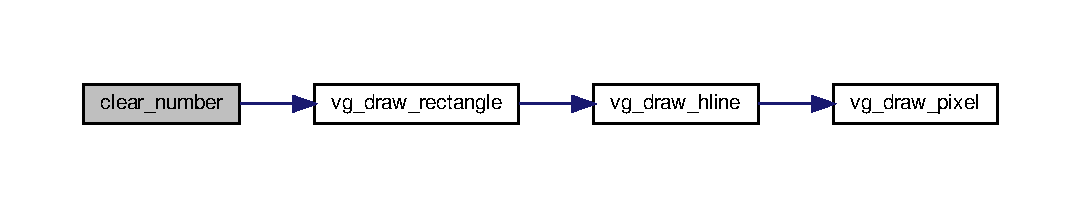
\includegraphics[width=350pt]{group__graphics_ga3a318192b1144825603071c57fdc4b8e_cgraph}
\end{center}
\end{figure}
Here is the caller graph for this function\+:\nopagebreak
\begin{figure}[H]
\begin{center}
\leavevmode
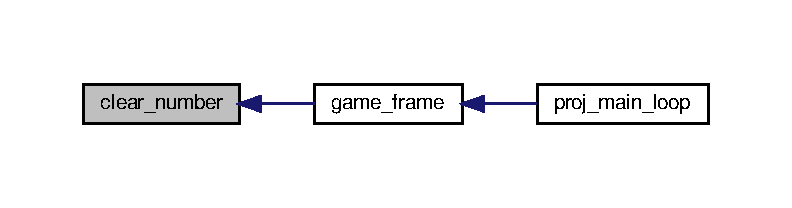
\includegraphics[width=350pt]{group__graphics_ga3a318192b1144825603071c57fdc4b8e_icgraph}
\end{center}
\end{figure}
\mbox{\Hypertarget{group__graphics_ga51ea06097c3bf68f7963901b0296bde6}\label{group__graphics_ga51ea06097c3bf68f7963901b0296bde6}} 
\index{graphics@{graphics}!clear\+\_\+text@{clear\+\_\+text}}
\index{clear\+\_\+text@{clear\+\_\+text}!graphics@{graphics}}
\subsubsection{\texorpdfstring{clear\+\_\+text()}{clear\_text()}}
{\footnotesize\ttfamily void() clear\+\_\+text (\begin{DoxyParamCaption}\item[{char $\ast$}]{str,  }\item[{int}]{x,  }\item[{int}]{y }\end{DoxyParamCaption})}



Clear the text drawn in the x,y position. 

Here is the call graph for this function\+:\nopagebreak
\begin{figure}[H]
\begin{center}
\leavevmode
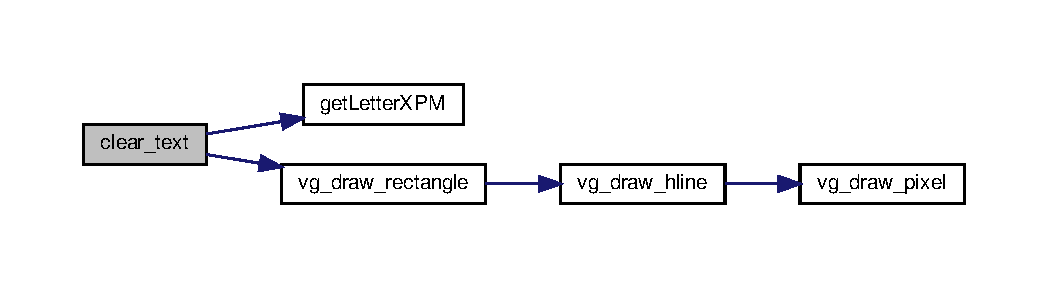
\includegraphics[width=350pt]{group__graphics_ga51ea06097c3bf68f7963901b0296bde6_cgraph}
\end{center}
\end{figure}
Here is the caller graph for this function\+:\nopagebreak
\begin{figure}[H]
\begin{center}
\leavevmode
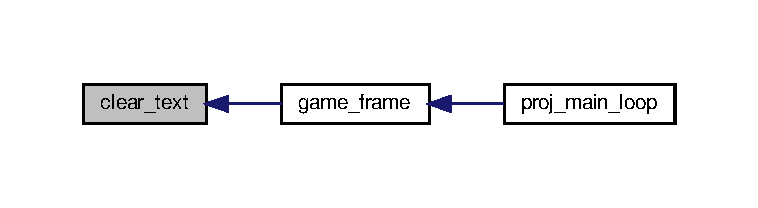
\includegraphics[width=350pt]{group__graphics_ga51ea06097c3bf68f7963901b0296bde6_icgraph}
\end{center}
\end{figure}
\mbox{\Hypertarget{group__graphics_gae70314d2e6e41dae20ce327a13929401}\label{group__graphics_gae70314d2e6e41dae20ce327a13929401}} 
\index{graphics@{graphics}!draw\+\_\+frame@{draw\+\_\+frame}}
\index{draw\+\_\+frame@{draw\+\_\+frame}!graphics@{graphics}}
\subsubsection{\texorpdfstring{draw\+\_\+frame()}{draw\_frame()}}
{\footnotesize\ttfamily void() draw\+\_\+frame (\begin{DoxyParamCaption}{ }\end{DoxyParamCaption})}



Draw video buffer into video memory. 

Here is the caller graph for this function\+:\nopagebreak
\begin{figure}[H]
\begin{center}
\leavevmode
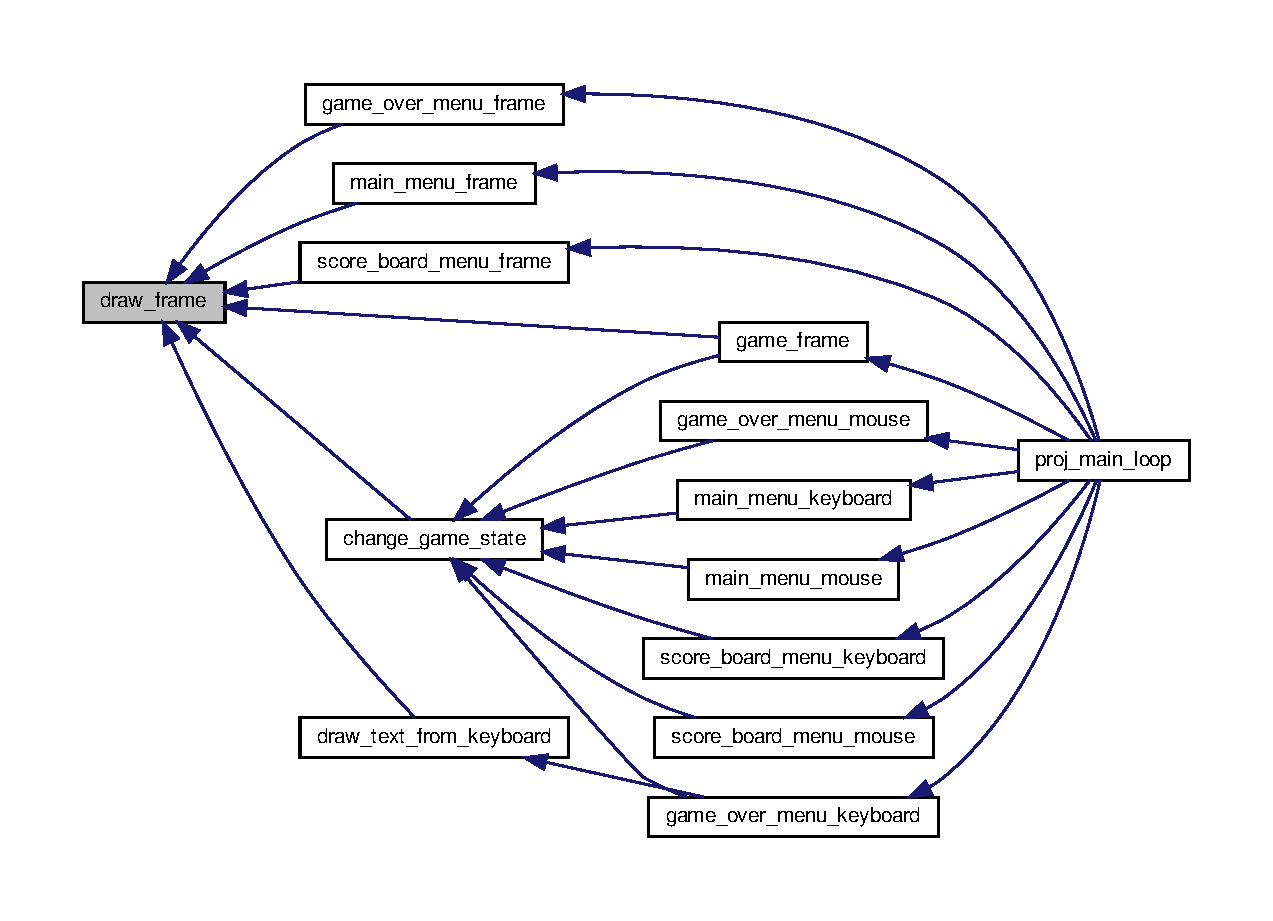
\includegraphics[width=350pt]{group__graphics_gae70314d2e6e41dae20ce327a13929401_icgraph}
\end{center}
\end{figure}
\mbox{\Hypertarget{group__graphics_ga7b24da519204bf650a1e98c993093e94}\label{group__graphics_ga7b24da519204bf650a1e98c993093e94}} 
\index{graphics@{graphics}!draw\+\_\+number@{draw\+\_\+number}}
\index{draw\+\_\+number@{draw\+\_\+number}!graphics@{graphics}}
\subsubsection{\texorpdfstring{draw\+\_\+number()}{draw\_number()}}
{\footnotesize\ttfamily void() draw\+\_\+number (\begin{DoxyParamCaption}\item[{int}]{n,  }\item[{int}]{x,  }\item[{int}]{y }\end{DoxyParamCaption})}



Draw a number into x,y position. 

Here is the call graph for this function\+:\nopagebreak
\begin{figure}[H]
\begin{center}
\leavevmode
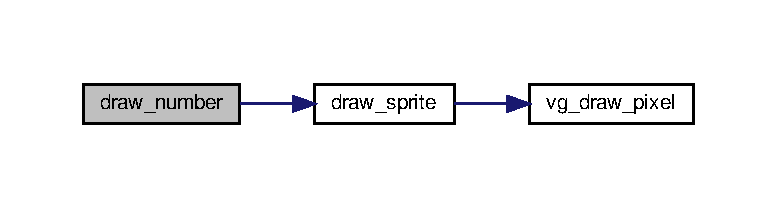
\includegraphics[width=350pt]{group__graphics_ga7b24da519204bf650a1e98c993093e94_cgraph}
\end{center}
\end{figure}
Here is the caller graph for this function\+:\nopagebreak
\begin{figure}[H]
\begin{center}
\leavevmode
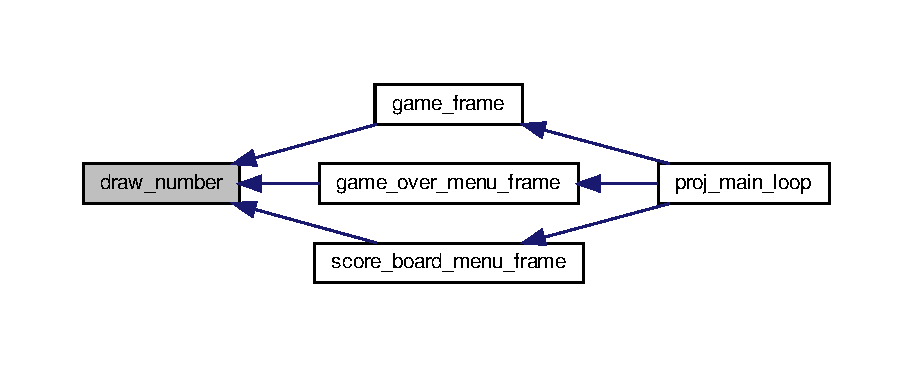
\includegraphics[width=350pt]{group__graphics_ga7b24da519204bf650a1e98c993093e94_icgraph}
\end{center}
\end{figure}
\mbox{\Hypertarget{group__graphics_ga08b3cc962ee64800e139310f91a3d4b4}\label{group__graphics_ga08b3cc962ee64800e139310f91a3d4b4}} 
\index{graphics@{graphics}!draw\+\_\+object@{draw\+\_\+object}}
\index{draw\+\_\+object@{draw\+\_\+object}!graphics@{graphics}}
\subsubsection{\texorpdfstring{draw\+\_\+object()}{draw\_object()}}
{\footnotesize\ttfamily int() draw\+\_\+object (\begin{DoxyParamCaption}\item[{\hyperlink{structObject}{Object}}]{object }\end{DoxyParamCaption})}



Draw a sprite in position (x,y), from struct object. 

Here is the call graph for this function\+:\nopagebreak
\begin{figure}[H]
\begin{center}
\leavevmode
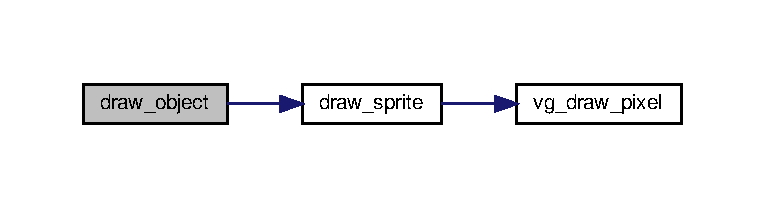
\includegraphics[width=350pt]{group__graphics_ga08b3cc962ee64800e139310f91a3d4b4_cgraph}
\end{center}
\end{figure}
Here is the caller graph for this function\+:\nopagebreak
\begin{figure}[H]
\begin{center}
\leavevmode
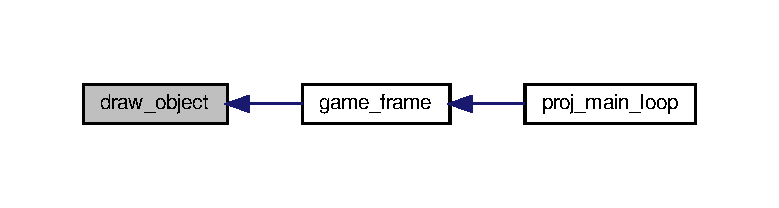
\includegraphics[width=350pt]{group__graphics_ga08b3cc962ee64800e139310f91a3d4b4_icgraph}
\end{center}
\end{figure}
\mbox{\Hypertarget{group__graphics_ga7f31f56ddc44fb5e02130bbe4a6c3927}\label{group__graphics_ga7f31f56ddc44fb5e02130bbe4a6c3927}} 
\index{graphics@{graphics}!draw\+\_\+sprite@{draw\+\_\+sprite}}
\index{draw\+\_\+sprite@{draw\+\_\+sprite}!graphics@{graphics}}
\subsubsection{\texorpdfstring{draw\+\_\+sprite()}{draw\_sprite()}}
{\footnotesize\ttfamily int() draw\+\_\+sprite (\begin{DoxyParamCaption}\item[{xpm\+\_\+image\+\_\+t}]{sprite,  }\item[{uint16\+\_\+t}]{x,  }\item[{uint16\+\_\+t}]{y }\end{DoxyParamCaption})}



Draw a sprite in position (x,y), from sprite. 

Here is the call graph for this function\+:
\nopagebreak
\begin{figure}[H]
\begin{center}
\leavevmode
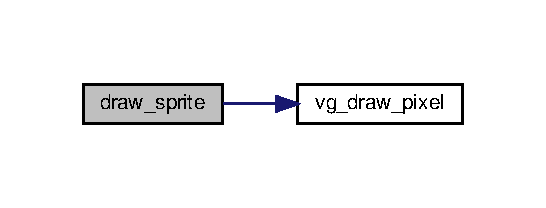
\includegraphics[width=262pt]{group__graphics_ga7f31f56ddc44fb5e02130bbe4a6c3927_cgraph}
\end{center}
\end{figure}
Here is the caller graph for this function\+:
\nopagebreak
\begin{figure}[H]
\begin{center}
\leavevmode
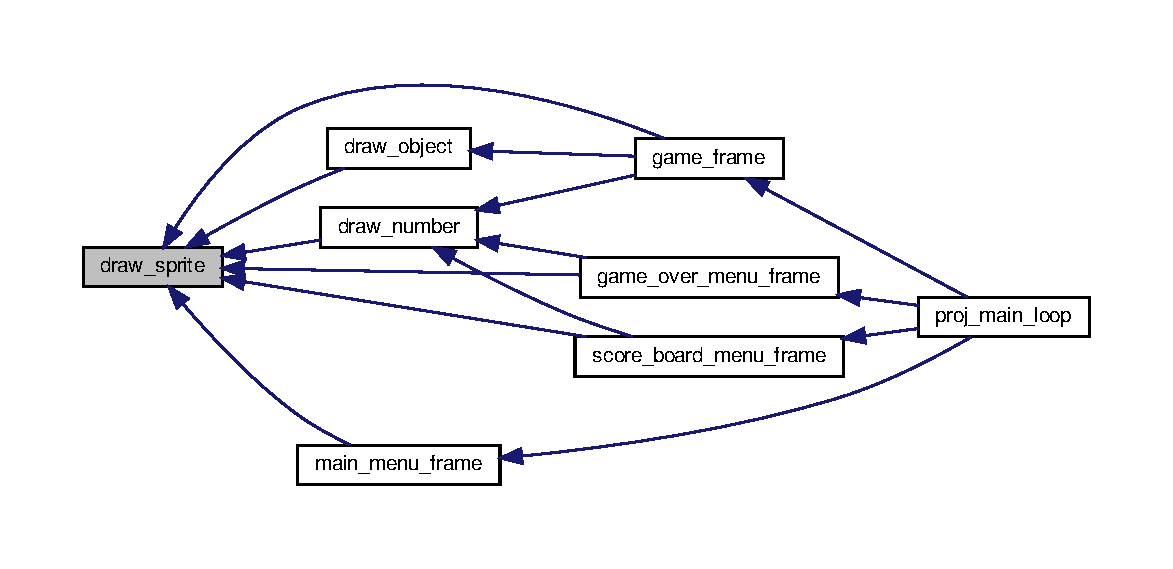
\includegraphics[width=350pt]{group__graphics_ga7f31f56ddc44fb5e02130bbe4a6c3927_icgraph}
\end{center}
\end{figure}
\mbox{\Hypertarget{group__graphics_gaf7d28831f1ffad3816101e473a54b9be}\label{group__graphics_gaf7d28831f1ffad3816101e473a54b9be}} 
\index{graphics@{graphics}!draw\+\_\+sprite\+\_\+xpm@{draw\+\_\+sprite\+\_\+xpm}}
\index{draw\+\_\+sprite\+\_\+xpm@{draw\+\_\+sprite\+\_\+xpm}!graphics@{graphics}}
\subsubsection{\texorpdfstring{draw\+\_\+sprite\+\_\+xpm()}{draw\_sprite\_xpm()}}
{\footnotesize\ttfamily int() draw\+\_\+sprite\+\_\+xpm (\begin{DoxyParamCaption}\item[{xpm\+\_\+map\+\_\+t}]{xpm,  }\item[{uint16\+\_\+t}]{x,  }\item[{uint16\+\_\+t}]{y }\end{DoxyParamCaption})}



Draw a sprite in position (x,y), from X\+PM. 

Here is the call graph for this function\+:
\nopagebreak
\begin{figure}[H]
\begin{center}
\leavevmode
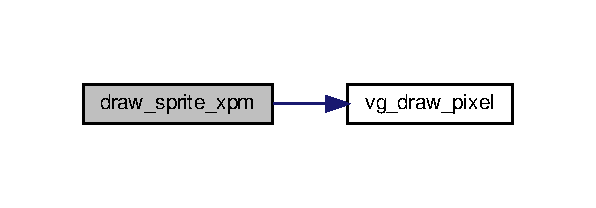
\includegraphics[width=286pt]{group__graphics_gaf7d28831f1ffad3816101e473a54b9be_cgraph}
\end{center}
\end{figure}
Here is the caller graph for this function\+:
\nopagebreak
\begin{figure}[H]
\begin{center}
\leavevmode
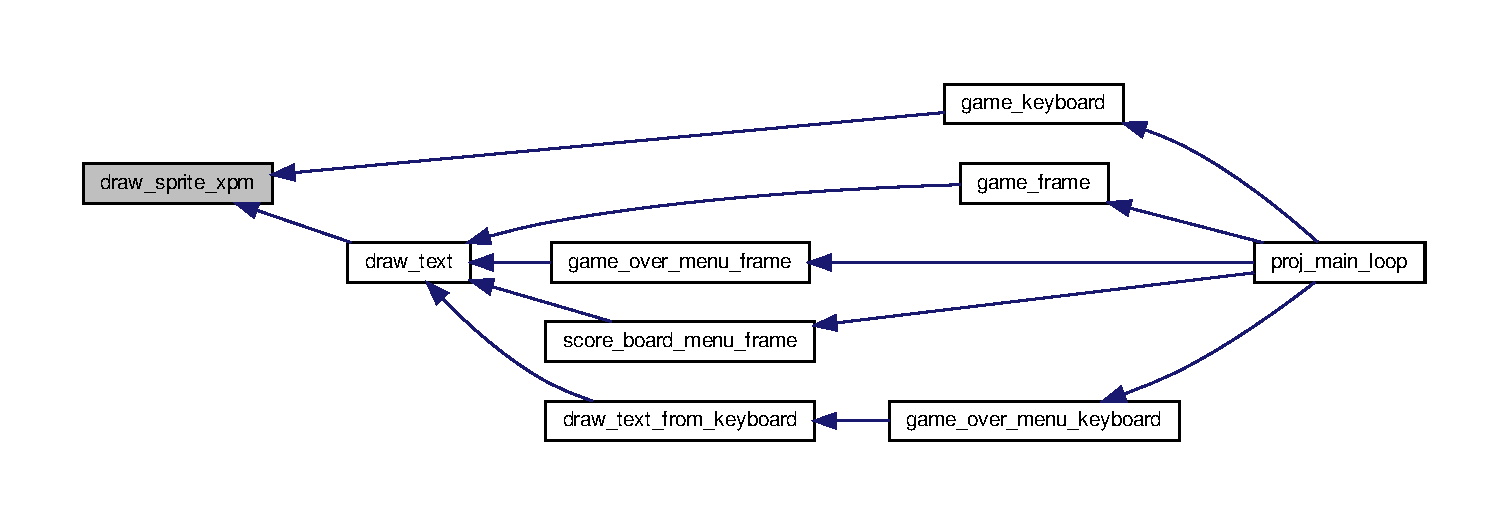
\includegraphics[width=350pt]{group__graphics_gaf7d28831f1ffad3816101e473a54b9be_icgraph}
\end{center}
\end{figure}
\mbox{\Hypertarget{group__graphics_ga37cbb1079da920cd529418d4a9f83ff2}\label{group__graphics_ga37cbb1079da920cd529418d4a9f83ff2}} 
\index{graphics@{graphics}!draw\+\_\+text@{draw\+\_\+text}}
\index{draw\+\_\+text@{draw\+\_\+text}!graphics@{graphics}}
\subsubsection{\texorpdfstring{draw\+\_\+text()}{draw\_text()}}
{\footnotesize\ttfamily void() draw\+\_\+text (\begin{DoxyParamCaption}\item[{char $\ast$}]{str,  }\item[{int}]{x,  }\item[{int}]{y }\end{DoxyParamCaption})}



Draw a text in the given position. 

Here is the call graph for this function\+:
\nopagebreak
\begin{figure}[H]
\begin{center}
\leavevmode
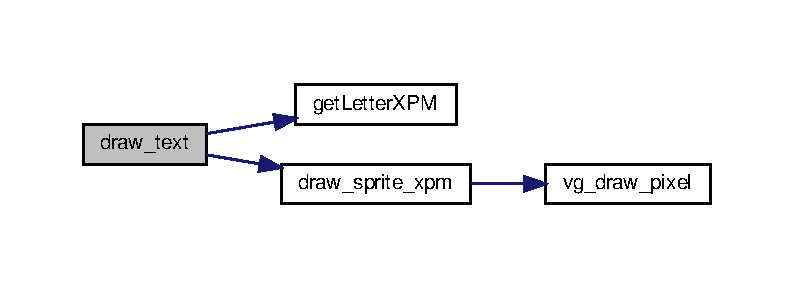
\includegraphics[width=350pt]{group__graphics_ga37cbb1079da920cd529418d4a9f83ff2_cgraph}
\end{center}
\end{figure}
Here is the caller graph for this function\+:
\nopagebreak
\begin{figure}[H]
\begin{center}
\leavevmode
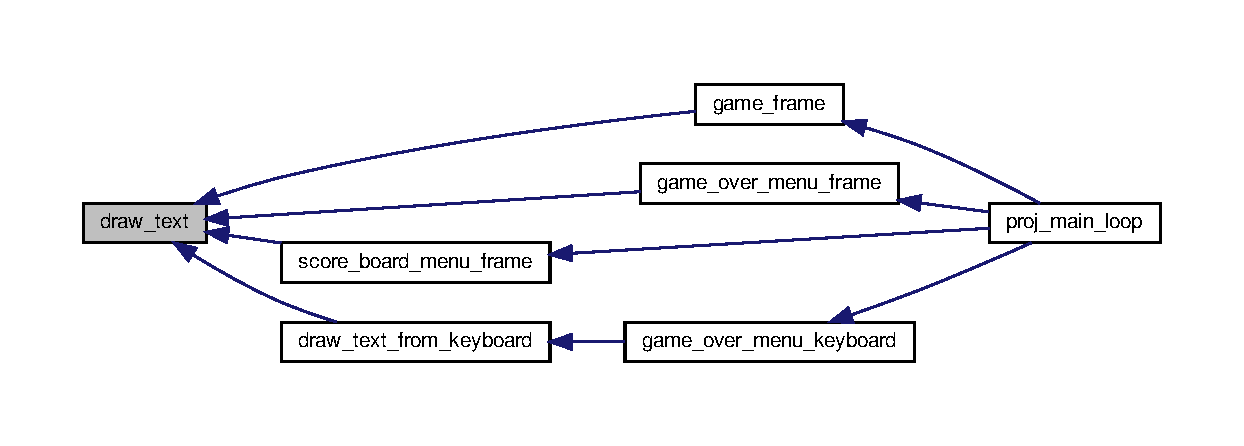
\includegraphics[width=350pt]{group__graphics_ga37cbb1079da920cd529418d4a9f83ff2_icgraph}
\end{center}
\end{figure}
\mbox{\Hypertarget{group__graphics_ga97ef658560a953fdb5a8ac8310b31516}\label{group__graphics_ga97ef658560a953fdb5a8ac8310b31516}} 
\index{graphics@{graphics}!fill\+\_\+bckgnd@{fill\+\_\+bckgnd}}
\index{fill\+\_\+bckgnd@{fill\+\_\+bckgnd}!graphics@{graphics}}
\subsubsection{\texorpdfstring{fill\+\_\+bckgnd()}{fill\_bckgnd()}}
{\footnotesize\ttfamily int() fill\+\_\+bckgnd (\begin{DoxyParamCaption}{ }\end{DoxyParamCaption})}



Fill the screen in black. 

Here is the call graph for this function\+:
\nopagebreak
\begin{figure}[H]
\begin{center}
\leavevmode
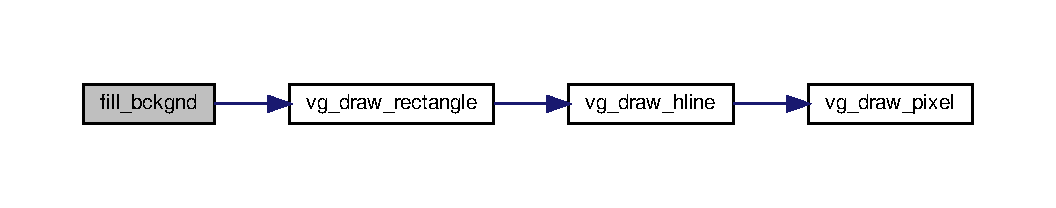
\includegraphics[width=350pt]{group__graphics_ga97ef658560a953fdb5a8ac8310b31516_cgraph}
\end{center}
\end{figure}
Here is the caller graph for this function\+:
\nopagebreak
\begin{figure}[H]
\begin{center}
\leavevmode
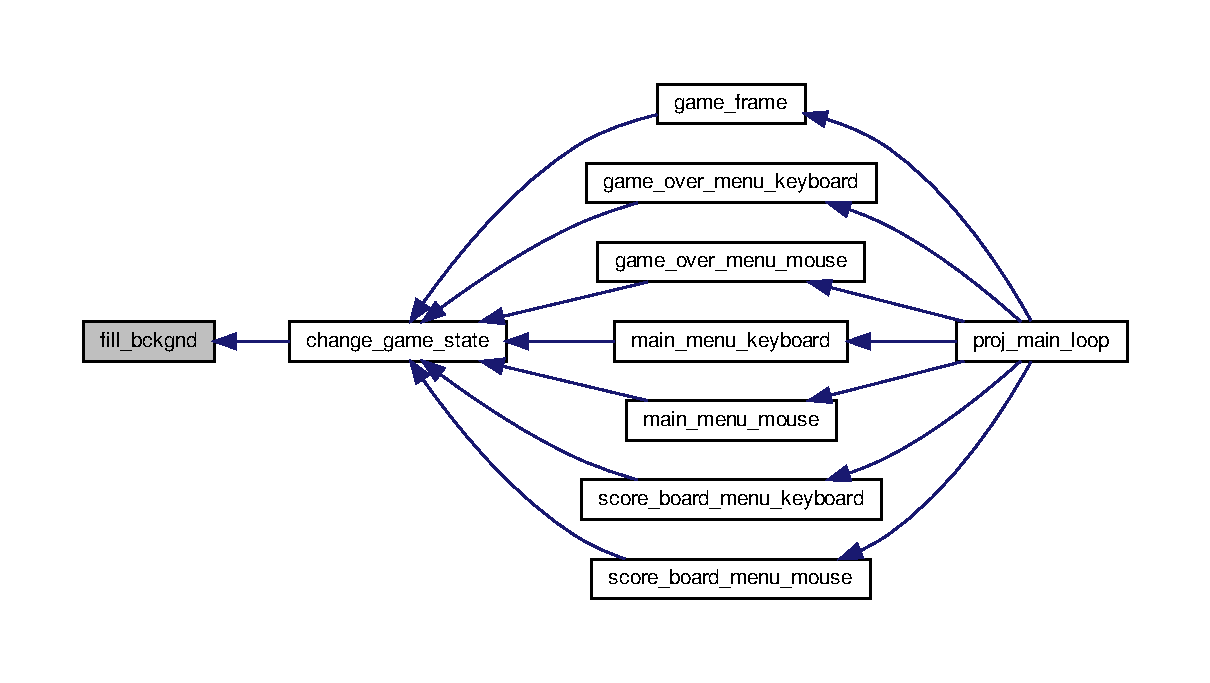
\includegraphics[width=350pt]{group__graphics_ga97ef658560a953fdb5a8ac8310b31516_icgraph}
\end{center}
\end{figure}
\mbox{\Hypertarget{group__graphics_ga427099c53976d605666e7e2b39238bb9}\label{group__graphics_ga427099c53976d605666e7e2b39238bb9}} 
\index{graphics@{graphics}!free\+\_\+buffer@{free\+\_\+buffer}}
\index{free\+\_\+buffer@{free\+\_\+buffer}!graphics@{graphics}}
\subsubsection{\texorpdfstring{free\+\_\+buffer()}{free\_buffer()}}
{\footnotesize\ttfamily void() free\+\_\+buffer (\begin{DoxyParamCaption}{ }\end{DoxyParamCaption})}



Dealocates video buffer. 

Here is the caller graph for this function\+:
\nopagebreak
\begin{figure}[H]
\begin{center}
\leavevmode
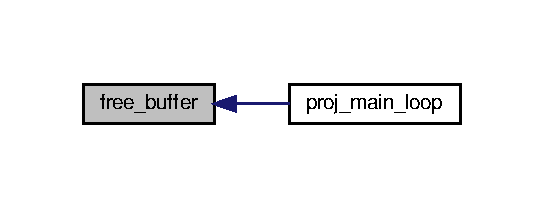
\includegraphics[width=261pt]{group__graphics_ga427099c53976d605666e7e2b39238bb9_icgraph}
\end{center}
\end{figure}
\mbox{\Hypertarget{group__graphics_gad93c2188e33c696ab1697dc05b320131}\label{group__graphics_gad93c2188e33c696ab1697dc05b320131}} 
\index{graphics@{graphics}!load\+\_\+numbers@{load\+\_\+numbers}}
\index{load\+\_\+numbers@{load\+\_\+numbers}!graphics@{graphics}}
\subsubsection{\texorpdfstring{load\+\_\+numbers()}{load\_numbers()}}
{\footnotesize\ttfamily void() load\+\_\+numbers (\begin{DoxyParamCaption}{ }\end{DoxyParamCaption})}



Load the number xpm into an array for better performance. 

Here is the call graph for this function\+:
\nopagebreak
\begin{figure}[H]
\begin{center}
\leavevmode
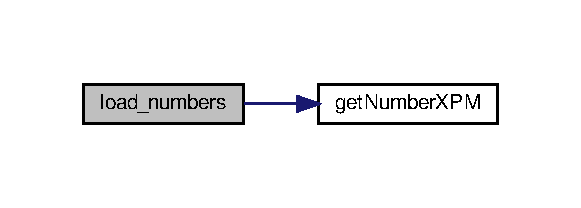
\includegraphics[width=279pt]{group__graphics_gad93c2188e33c696ab1697dc05b320131_cgraph}
\end{center}
\end{figure}
Here is the caller graph for this function\+:
\nopagebreak
\begin{figure}[H]
\begin{center}
\leavevmode
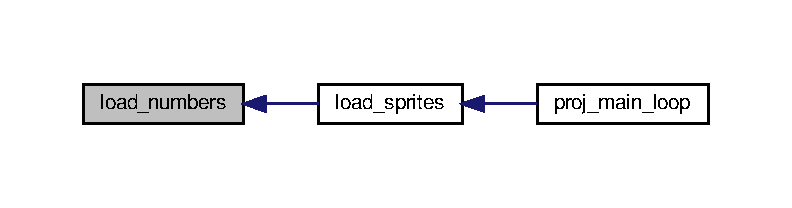
\includegraphics[width=350pt]{group__graphics_gad93c2188e33c696ab1697dc05b320131_icgraph}
\end{center}
\end{figure}
\mbox{\Hypertarget{group__graphics_ga1677f4b59f9e0584d82e0b655e4b7fc9}\label{group__graphics_ga1677f4b59f9e0584d82e0b655e4b7fc9}} 
\index{graphics@{graphics}!vg\+\_\+draw\+\_\+hline@{vg\+\_\+draw\+\_\+hline}}
\index{vg\+\_\+draw\+\_\+hline@{vg\+\_\+draw\+\_\+hline}!graphics@{graphics}}
\subsubsection{\texorpdfstring{vg\+\_\+draw\+\_\+hline()}{vg\_draw\_hline()}}
{\footnotesize\ttfamily int() vg\+\_\+draw\+\_\+hline (\begin{DoxyParamCaption}\item[{uint16\+\_\+t}]{x,  }\item[{uint16\+\_\+t}]{y,  }\item[{uint16\+\_\+t}]{width,  }\item[{uint32\+\_\+t}]{color }\end{DoxyParamCaption})}



Draw horizontal line in given x,y position with given width and color. 

Here is the call graph for this function\+:
\nopagebreak
\begin{figure}[H]
\begin{center}
\leavevmode
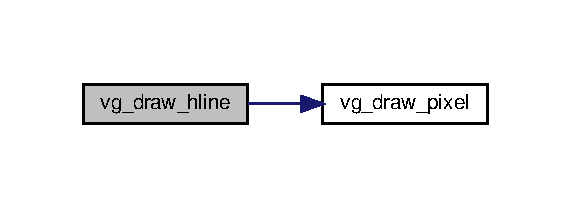
\includegraphics[width=274pt]{group__graphics_ga1677f4b59f9e0584d82e0b655e4b7fc9_cgraph}
\end{center}
\end{figure}
Here is the caller graph for this function\+:
\nopagebreak
\begin{figure}[H]
\begin{center}
\leavevmode
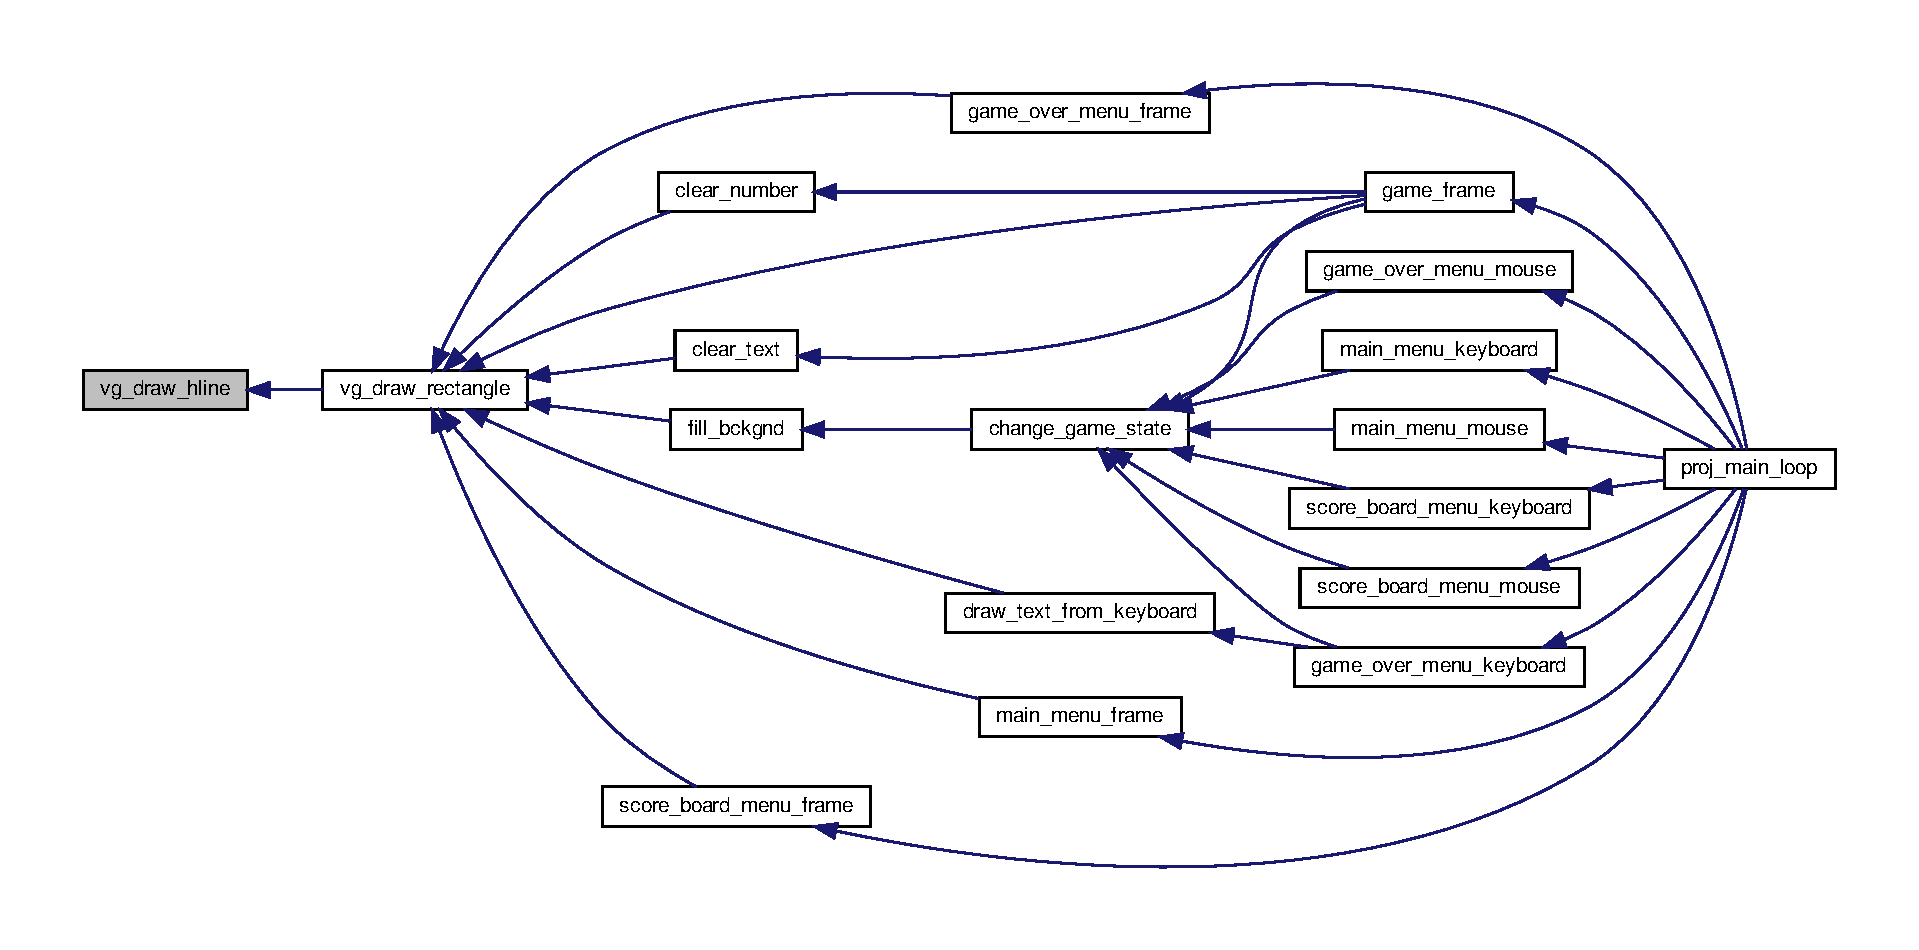
\includegraphics[width=350pt]{group__graphics_ga1677f4b59f9e0584d82e0b655e4b7fc9_icgraph}
\end{center}
\end{figure}
\mbox{\Hypertarget{group__graphics_ga08c498ffeb0a3962e3b7711b57397741}\label{group__graphics_ga08c498ffeb0a3962e3b7711b57397741}} 
\index{graphics@{graphics}!vg\+\_\+draw\+\_\+pixel@{vg\+\_\+draw\+\_\+pixel}}
\index{vg\+\_\+draw\+\_\+pixel@{vg\+\_\+draw\+\_\+pixel}!graphics@{graphics}}
\subsubsection{\texorpdfstring{vg\+\_\+draw\+\_\+pixel()}{vg\_draw\_pixel()}}
{\footnotesize\ttfamily int() vg\+\_\+draw\+\_\+pixel (\begin{DoxyParamCaption}\item[{uint16\+\_\+t}]{x,  }\item[{uint16\+\_\+t}]{y,  }\item[{uint32\+\_\+t}]{color }\end{DoxyParamCaption})}



Turns the given x,y position pixel to the given color. 

Here is the caller graph for this function\+:
\nopagebreak
\begin{figure}[H]
\begin{center}
\leavevmode
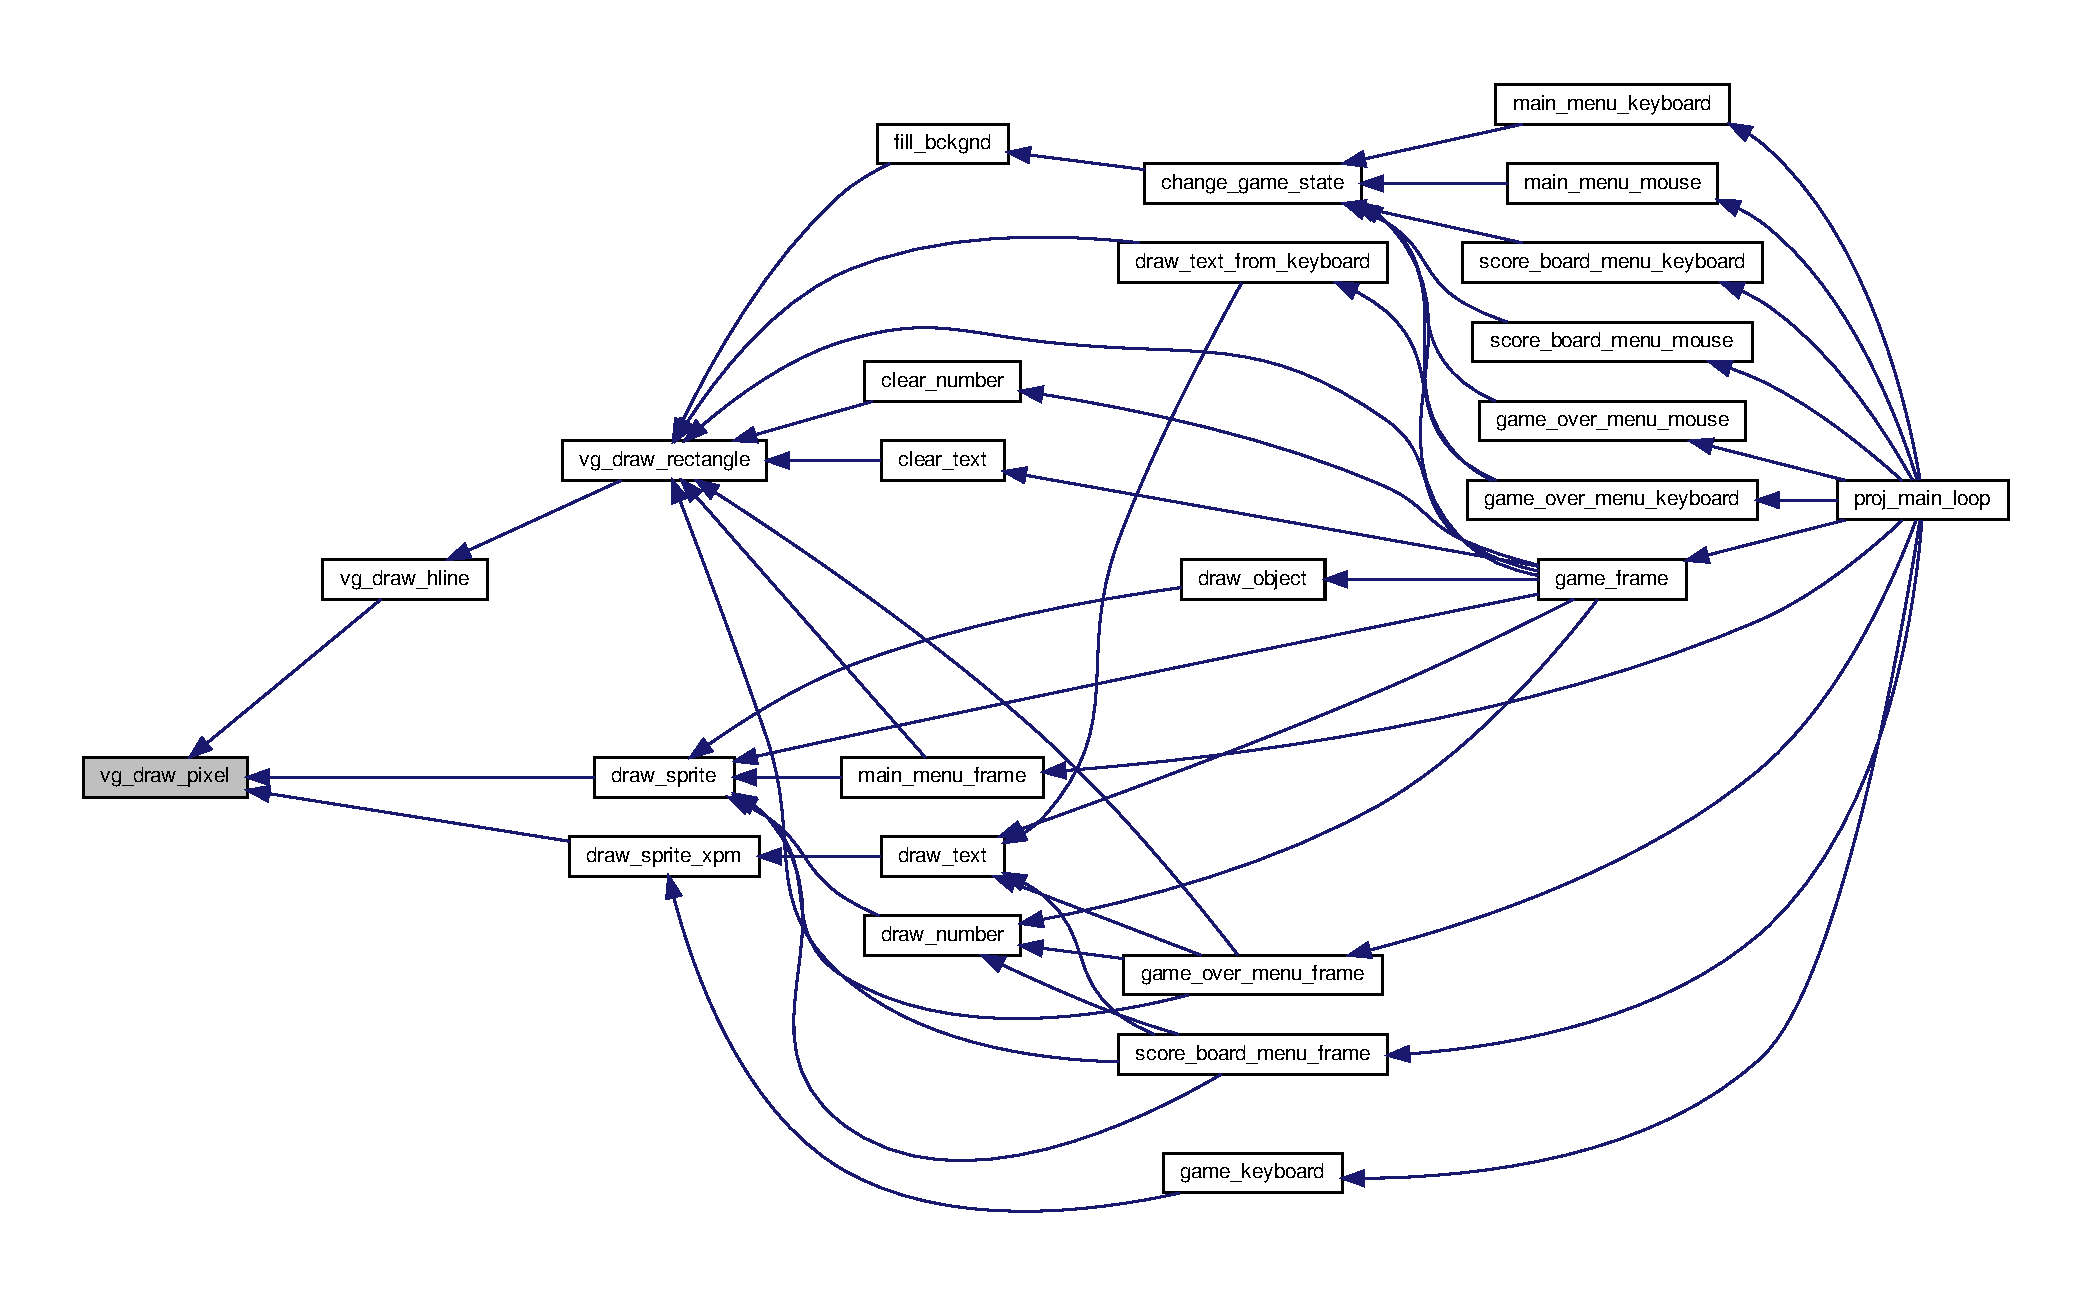
\includegraphics[width=350pt]{group__graphics_ga08c498ffeb0a3962e3b7711b57397741_icgraph}
\end{center}
\end{figure}
\mbox{\Hypertarget{group__graphics_ga99d2da2559e11200c6b40c469e9977ec}\label{group__graphics_ga99d2da2559e11200c6b40c469e9977ec}} 
\index{graphics@{graphics}!vg\+\_\+draw\+\_\+rectangle@{vg\+\_\+draw\+\_\+rectangle}}
\index{vg\+\_\+draw\+\_\+rectangle@{vg\+\_\+draw\+\_\+rectangle}!graphics@{graphics}}
\subsubsection{\texorpdfstring{vg\+\_\+draw\+\_\+rectangle()}{vg\_draw\_rectangle()}}
{\footnotesize\ttfamily int() vg\+\_\+draw\+\_\+rectangle (\begin{DoxyParamCaption}\item[{uint16\+\_\+t}]{x,  }\item[{uint16\+\_\+t}]{y,  }\item[{uint16\+\_\+t}]{width,  }\item[{uint16\+\_\+t}]{height,  }\item[{uint32\+\_\+t}]{color }\end{DoxyParamCaption})}



Draws a rectangle of given color with given size in given position. 

Here is the call graph for this function\+:
\nopagebreak
\begin{figure}[H]
\begin{center}
\leavevmode
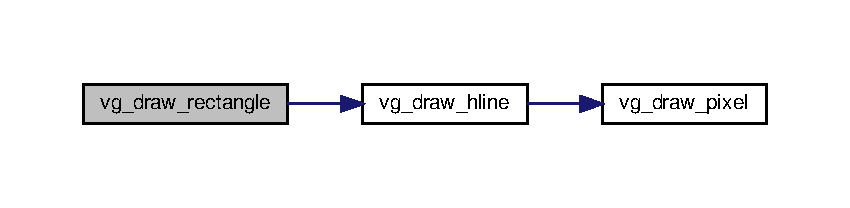
\includegraphics[width=350pt]{group__graphics_ga99d2da2559e11200c6b40c469e9977ec_cgraph}
\end{center}
\end{figure}
Here is the caller graph for this function\+:
\nopagebreak
\begin{figure}[H]
\begin{center}
\leavevmode
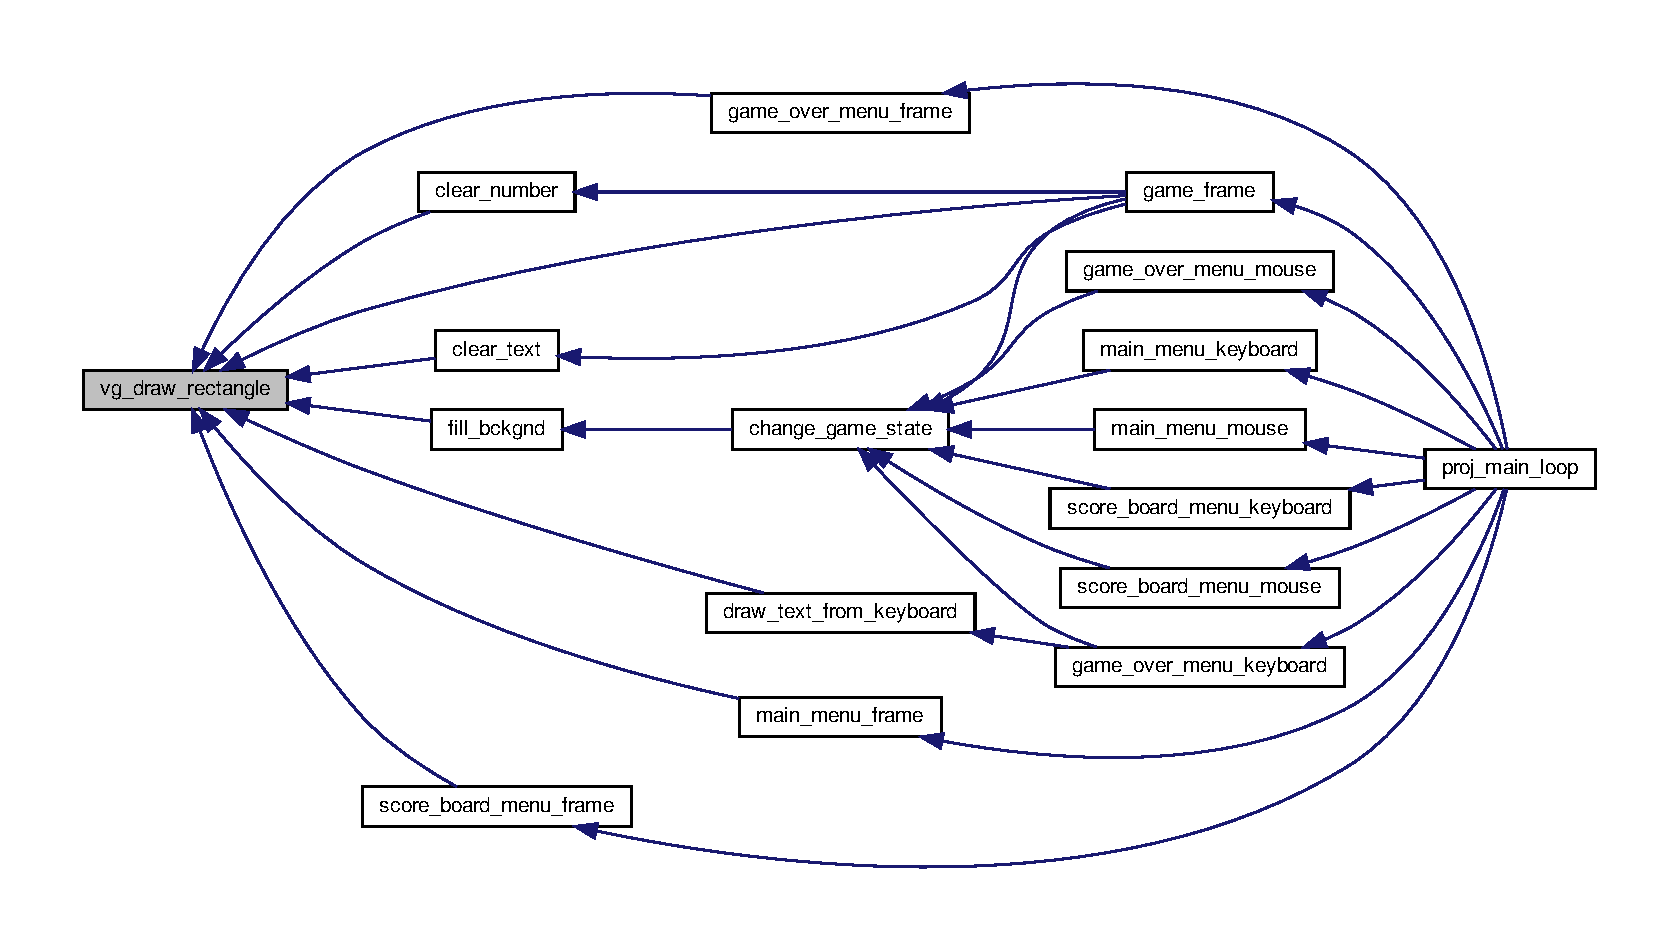
\includegraphics[width=350pt]{group__graphics_ga99d2da2559e11200c6b40c469e9977ec_icgraph}
\end{center}
\end{figure}
\mbox{\Hypertarget{group__graphics_gac34ed31db6d6ef68b7167a0c024cac2b}\label{group__graphics_gac34ed31db6d6ef68b7167a0c024cac2b}} 
\index{graphics@{graphics}!vg\+\_\+enter@{vg\+\_\+enter}}
\index{vg\+\_\+enter@{vg\+\_\+enter}!graphics@{graphics}}
\subsubsection{\texorpdfstring{vg\+\_\+enter()}{vg\_enter()}}
{\footnotesize\ttfamily int() vg\+\_\+enter (\begin{DoxyParamCaption}\item[{uint16\+\_\+t}]{mode }\end{DoxyParamCaption})}



Enters video mode in the given mode. 

\mbox{\Hypertarget{group__graphics_gaa6c1ff5024cd4d15e476bce487584daa}\label{group__graphics_gaa6c1ff5024cd4d15e476bce487584daa}} 
\index{graphics@{graphics}!vg\+\_\+init@{vg\+\_\+init}}
\index{vg\+\_\+init@{vg\+\_\+init}!graphics@{graphics}}
\subsubsection{\texorpdfstring{vg\+\_\+init()}{vg\_init()}}
{\footnotesize\ttfamily void$\ast$() vg\+\_\+init (\begin{DoxyParamCaption}\item[{uint16\+\_\+t}]{mode }\end{DoxyParamCaption})}



Initializes video grafics variables. 

Here is the caller graph for this function\+:
\nopagebreak
\begin{figure}[H]
\begin{center}
\leavevmode
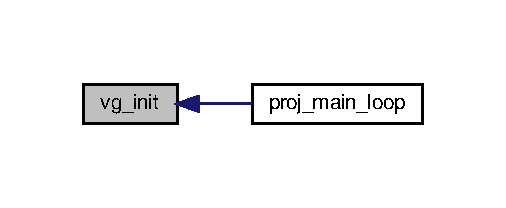
\includegraphics[width=243pt]{group__graphics_gaa6c1ff5024cd4d15e476bce487584daa_icgraph}
\end{center}
\end{figure}


\subsection{Variable Documentation}
\mbox{\Hypertarget{group__graphics_ga5aa03a801f01a5140c299908a06c47cd}\label{group__graphics_ga5aa03a801f01a5140c299908a06c47cd}} 
\index{graphics@{graphics}!numbers\+\_\+sprites@{numbers\+\_\+sprites}}
\index{numbers\+\_\+sprites@{numbers\+\_\+sprites}!graphics@{graphics}}
\subsubsection{\texorpdfstring{numbers\+\_\+sprites}{numbers\_sprites}}
{\footnotesize\ttfamily xpm\+\_\+image\+\_\+t numbers\+\_\+sprites\mbox{[}10\mbox{]}}



Array with sprites of the numbers from 0 to 9. 

\mbox{\Hypertarget{group__graphics_ga505fdb0bbcbe5f0d3a5c4a3d1190401a}\label{group__graphics_ga505fdb0bbcbe5f0d3a5c4a3d1190401a}} 
\index{graphics@{graphics}!vd\+\_\+mode@{vd\+\_\+mode}}
\index{vd\+\_\+mode@{vd\+\_\+mode}!graphics@{graphics}}
\subsubsection{\texorpdfstring{vd\+\_\+mode}{vd\_mode}}
{\footnotesize\ttfamily uint16\+\_\+t vd\+\_\+mode}


\hypertarget{group__i8254}{}\section{i8254}
\label{group__i8254}\index{i8254@{i8254}}
\subsection*{Macros}
\begin{DoxyCompactItemize}
\item 
\#define \hyperlink{group__i8254_gacf926951944b6cf370b7229ebd50dd8b}{T\+I\+M\+E\+R\+\_\+\+F\+R\+EQ}~1193182
\begin{DoxyCompactList}\small\item\em clock frequency for timer in PC and AT \end{DoxyCompactList}\item 
\#define \hyperlink{group__i8254_ga30bf84c312af248cb81bb224e09f9ba8}{T\+I\+M\+E\+R0\+\_\+\+I\+RQ}~0
\begin{DoxyCompactList}\small\item\em Timer 0 I\+RQ line. \end{DoxyCompactList}\item 
\#define \hyperlink{group__i8254_gacc9ff9df4a9674a1ce9ba08fc4a4679e}{T\+I\+M\+E\+R\+\_\+0}~0x40
\begin{DoxyCompactList}\small\item\em Timer 0 count register. \end{DoxyCompactList}\item 
\#define \hyperlink{group__i8254_gac62c99c2a9289891c1b83052242cca49}{T\+I\+M\+E\+R\+\_\+1}~0x41
\begin{DoxyCompactList}\small\item\em Timer 1 count register. \end{DoxyCompactList}\item 
\#define \hyperlink{group__i8254_ga1f34f18ad0ab8cace46b615773b48735}{T\+I\+M\+E\+R\+\_\+2}~0x42
\begin{DoxyCompactList}\small\item\em Timer 2 count register. \end{DoxyCompactList}\item 
\#define \hyperlink{group__i8254_ga282832448fb0281ef53d243c1cd48491}{T\+I\+M\+E\+R\+\_\+\+C\+T\+RL}~0x43
\begin{DoxyCompactList}\small\item\em Control register. \end{DoxyCompactList}\item 
\#define \hyperlink{group__i8254_ga51b3a5e3d4811ca063fe25e35560ab40}{S\+P\+E\+A\+K\+E\+R\+\_\+\+C\+T\+RL}~0x61
\begin{DoxyCompactList}\small\item\em Register for speaker control. \end{DoxyCompactList}\item 
\#define \hyperlink{group__i8254_ga6a4822642d40c248435692324a818010}{T\+I\+M\+E\+R\+\_\+\+S\+E\+L0}~0x00
\begin{DoxyCompactList}\small\item\em Control Word for Timer 0. \end{DoxyCompactList}\item 
\#define \hyperlink{group__i8254_ga8349623fd8d99f9cc5d8ae29d78594fc}{T\+I\+M\+E\+R\+\_\+\+S\+E\+L1}~B\+IT(6)
\begin{DoxyCompactList}\small\item\em Control Word for Timer 1. \end{DoxyCompactList}\item 
\#define \hyperlink{group__i8254_ga142a255de0dbc48aeabd45fc10c33672}{T\+I\+M\+E\+R\+\_\+\+S\+E\+L2}~B\+IT(7)
\begin{DoxyCompactList}\small\item\em Control Word for Timer 2. \end{DoxyCompactList}\item 
\#define \hyperlink{group__i8254_ga4c2eecbfb96744a9c2af71dba75ecb18}{T\+I\+M\+E\+R\+\_\+\+R\+B\+\_\+\+C\+MD}~(B\+IT(7) $\vert$ B\+IT(6))
\begin{DoxyCompactList}\small\item\em Read Back Command. \end{DoxyCompactList}\item 
\#define \hyperlink{group__i8254_gac18cb814ebd0d67235392c330e0e3504}{T\+I\+M\+E\+R\+\_\+\+L\+SB}~B\+IT(4)
\begin{DoxyCompactList}\small\item\em Initialize Counter L\+SB only. \end{DoxyCompactList}\item 
\#define \hyperlink{group__i8254_ga2a8a6d363c612d756cd8d78480f7cd04}{T\+I\+M\+E\+R\+\_\+\+M\+SB}~B\+IT(5)
\begin{DoxyCompactList}\small\item\em Initialize Counter M\+SB only. \end{DoxyCompactList}\item 
\#define \hyperlink{group__i8254_ga8c0f1933323274c765e23837e4fbc8c7}{T\+I\+M\+E\+R\+\_\+\+L\+S\+B\+\_\+\+M\+SB}~(\hyperlink{group__i8254_gac18cb814ebd0d67235392c330e0e3504}{T\+I\+M\+E\+R\+\_\+\+L\+SB} $\vert$ \hyperlink{group__i8254_ga2a8a6d363c612d756cd8d78480f7cd04}{T\+I\+M\+E\+R\+\_\+\+M\+SB})
\begin{DoxyCompactList}\small\item\em Initialize L\+SB first and M\+SB afterwards. \end{DoxyCompactList}\item 
\#define \hyperlink{group__i8254_ga4745cbf21da3d3fea5dbb080b2b73bac}{T\+I\+M\+E\+R\+\_\+\+S\+Q\+R\+\_\+\+W\+A\+VE}~(B\+IT(2) $\vert$ B\+IT(1))
\begin{DoxyCompactList}\small\item\em Mode 3\+: square wave generator. \end{DoxyCompactList}\item 
\#define \hyperlink{group__i8254_ga5d4449e0fa1cf4a4d107a48a04a1265f}{T\+I\+M\+E\+R\+\_\+\+R\+A\+T\+E\+\_\+\+G\+EN}~B\+IT(2)
\begin{DoxyCompactList}\small\item\em Mode 2\+: rate generator. \end{DoxyCompactList}\item 
\#define \hyperlink{group__i8254_ga325b992a371d5d981c4eceff42fa5956}{T\+I\+M\+E\+R\+\_\+\+B\+CD}~0x01
\begin{DoxyCompactList}\small\item\em Count in B\+CD. \end{DoxyCompactList}\item 
\#define \hyperlink{group__i8254_gad2913dcf2f91453317bd035589ac0a7d}{T\+I\+M\+E\+R\+\_\+\+B\+IN}~0x00
\begin{DoxyCompactList}\small\item\em Count in binary. \end{DoxyCompactList}\item 
\#define \hyperlink{group__i8254_ga6c248216df24b5e9d907d126d80bd195}{T\+I\+M\+E\+R\+\_\+\+R\+B\+\_\+\+C\+O\+U\+N\+T\+\_\+}~B\+IT(5)
\item 
\#define \hyperlink{group__i8254_ga08b4952bb7058684a3f8f66be04dd45e}{T\+I\+M\+E\+R\+\_\+\+R\+B\+\_\+\+S\+T\+A\+T\+U\+S\+\_\+}~B\+IT(4)
\item 
\#define \hyperlink{group__i8254_gaf598b17740e07842a0545af512714711}{T\+I\+M\+E\+R\+\_\+\+R\+B\+\_\+\+S\+EL}(n)~B\+IT((n) + 1)
\end{DoxyCompactItemize}


\subsection{Detailed Description}
Constants for programming the i8254 Timer. Needs to be completed. 

\subsection{Macro Definition Documentation}
\mbox{\Hypertarget{group__i8254_ga51b3a5e3d4811ca063fe25e35560ab40}\label{group__i8254_ga51b3a5e3d4811ca063fe25e35560ab40}} 
\index{i8254@{i8254}!S\+P\+E\+A\+K\+E\+R\+\_\+\+C\+T\+RL@{S\+P\+E\+A\+K\+E\+R\+\_\+\+C\+T\+RL}}
\index{S\+P\+E\+A\+K\+E\+R\+\_\+\+C\+T\+RL@{S\+P\+E\+A\+K\+E\+R\+\_\+\+C\+T\+RL}!i8254@{i8254}}
\subsubsection{\texorpdfstring{S\+P\+E\+A\+K\+E\+R\+\_\+\+C\+T\+RL}{SPEAKER\_CTRL}}
{\footnotesize\ttfamily \#define S\+P\+E\+A\+K\+E\+R\+\_\+\+C\+T\+RL~0x61}



Register for speaker control. 

\mbox{\Hypertarget{group__i8254_ga30bf84c312af248cb81bb224e09f9ba8}\label{group__i8254_ga30bf84c312af248cb81bb224e09f9ba8}} 
\index{i8254@{i8254}!T\+I\+M\+E\+R0\+\_\+\+I\+RQ@{T\+I\+M\+E\+R0\+\_\+\+I\+RQ}}
\index{T\+I\+M\+E\+R0\+\_\+\+I\+RQ@{T\+I\+M\+E\+R0\+\_\+\+I\+RQ}!i8254@{i8254}}
\subsubsection{\texorpdfstring{T\+I\+M\+E\+R0\+\_\+\+I\+RQ}{TIMER0\_IRQ}}
{\footnotesize\ttfamily \#define T\+I\+M\+E\+R0\+\_\+\+I\+RQ~0}



Timer 0 I\+RQ line. 

\mbox{\Hypertarget{group__i8254_gacc9ff9df4a9674a1ce9ba08fc4a4679e}\label{group__i8254_gacc9ff9df4a9674a1ce9ba08fc4a4679e}} 
\index{i8254@{i8254}!T\+I\+M\+E\+R\+\_\+0@{T\+I\+M\+E\+R\+\_\+0}}
\index{T\+I\+M\+E\+R\+\_\+0@{T\+I\+M\+E\+R\+\_\+0}!i8254@{i8254}}
\subsubsection{\texorpdfstring{T\+I\+M\+E\+R\+\_\+0}{TIMER\_0}}
{\footnotesize\ttfamily \#define T\+I\+M\+E\+R\+\_\+0~0x40}



Timer 0 count register. 

\mbox{\Hypertarget{group__i8254_gac62c99c2a9289891c1b83052242cca49}\label{group__i8254_gac62c99c2a9289891c1b83052242cca49}} 
\index{i8254@{i8254}!T\+I\+M\+E\+R\+\_\+1@{T\+I\+M\+E\+R\+\_\+1}}
\index{T\+I\+M\+E\+R\+\_\+1@{T\+I\+M\+E\+R\+\_\+1}!i8254@{i8254}}
\subsubsection{\texorpdfstring{T\+I\+M\+E\+R\+\_\+1}{TIMER\_1}}
{\footnotesize\ttfamily \#define T\+I\+M\+E\+R\+\_\+1~0x41}



Timer 1 count register. 

\mbox{\Hypertarget{group__i8254_ga1f34f18ad0ab8cace46b615773b48735}\label{group__i8254_ga1f34f18ad0ab8cace46b615773b48735}} 
\index{i8254@{i8254}!T\+I\+M\+E\+R\+\_\+2@{T\+I\+M\+E\+R\+\_\+2}}
\index{T\+I\+M\+E\+R\+\_\+2@{T\+I\+M\+E\+R\+\_\+2}!i8254@{i8254}}
\subsubsection{\texorpdfstring{T\+I\+M\+E\+R\+\_\+2}{TIMER\_2}}
{\footnotesize\ttfamily \#define T\+I\+M\+E\+R\+\_\+2~0x42}



Timer 2 count register. 

\mbox{\Hypertarget{group__i8254_ga325b992a371d5d981c4eceff42fa5956}\label{group__i8254_ga325b992a371d5d981c4eceff42fa5956}} 
\index{i8254@{i8254}!T\+I\+M\+E\+R\+\_\+\+B\+CD@{T\+I\+M\+E\+R\+\_\+\+B\+CD}}
\index{T\+I\+M\+E\+R\+\_\+\+B\+CD@{T\+I\+M\+E\+R\+\_\+\+B\+CD}!i8254@{i8254}}
\subsubsection{\texorpdfstring{T\+I\+M\+E\+R\+\_\+\+B\+CD}{TIMER\_BCD}}
{\footnotesize\ttfamily \#define T\+I\+M\+E\+R\+\_\+\+B\+CD~0x01}



Count in B\+CD. 

\mbox{\Hypertarget{group__i8254_gad2913dcf2f91453317bd035589ac0a7d}\label{group__i8254_gad2913dcf2f91453317bd035589ac0a7d}} 
\index{i8254@{i8254}!T\+I\+M\+E\+R\+\_\+\+B\+IN@{T\+I\+M\+E\+R\+\_\+\+B\+IN}}
\index{T\+I\+M\+E\+R\+\_\+\+B\+IN@{T\+I\+M\+E\+R\+\_\+\+B\+IN}!i8254@{i8254}}
\subsubsection{\texorpdfstring{T\+I\+M\+E\+R\+\_\+\+B\+IN}{TIMER\_BIN}}
{\footnotesize\ttfamily \#define T\+I\+M\+E\+R\+\_\+\+B\+IN~0x00}



Count in binary. 

\mbox{\Hypertarget{group__i8254_ga282832448fb0281ef53d243c1cd48491}\label{group__i8254_ga282832448fb0281ef53d243c1cd48491}} 
\index{i8254@{i8254}!T\+I\+M\+E\+R\+\_\+\+C\+T\+RL@{T\+I\+M\+E\+R\+\_\+\+C\+T\+RL}}
\index{T\+I\+M\+E\+R\+\_\+\+C\+T\+RL@{T\+I\+M\+E\+R\+\_\+\+C\+T\+RL}!i8254@{i8254}}
\subsubsection{\texorpdfstring{T\+I\+M\+E\+R\+\_\+\+C\+T\+RL}{TIMER\_CTRL}}
{\footnotesize\ttfamily \#define T\+I\+M\+E\+R\+\_\+\+C\+T\+RL~0x43}



Control register. 

\mbox{\Hypertarget{group__i8254_gacf926951944b6cf370b7229ebd50dd8b}\label{group__i8254_gacf926951944b6cf370b7229ebd50dd8b}} 
\index{i8254@{i8254}!T\+I\+M\+E\+R\+\_\+\+F\+R\+EQ@{T\+I\+M\+E\+R\+\_\+\+F\+R\+EQ}}
\index{T\+I\+M\+E\+R\+\_\+\+F\+R\+EQ@{T\+I\+M\+E\+R\+\_\+\+F\+R\+EQ}!i8254@{i8254}}
\subsubsection{\texorpdfstring{T\+I\+M\+E\+R\+\_\+\+F\+R\+EQ}{TIMER\_FREQ}}
{\footnotesize\ttfamily \#define T\+I\+M\+E\+R\+\_\+\+F\+R\+EQ~1193182}



clock frequency for timer in PC and AT 

\mbox{\Hypertarget{group__i8254_gac18cb814ebd0d67235392c330e0e3504}\label{group__i8254_gac18cb814ebd0d67235392c330e0e3504}} 
\index{i8254@{i8254}!T\+I\+M\+E\+R\+\_\+\+L\+SB@{T\+I\+M\+E\+R\+\_\+\+L\+SB}}
\index{T\+I\+M\+E\+R\+\_\+\+L\+SB@{T\+I\+M\+E\+R\+\_\+\+L\+SB}!i8254@{i8254}}
\subsubsection{\texorpdfstring{T\+I\+M\+E\+R\+\_\+\+L\+SB}{TIMER\_LSB}}
{\footnotesize\ttfamily \#define T\+I\+M\+E\+R\+\_\+\+L\+SB~B\+IT(4)}



Initialize Counter L\+SB only. 

\mbox{\Hypertarget{group__i8254_ga8c0f1933323274c765e23837e4fbc8c7}\label{group__i8254_ga8c0f1933323274c765e23837e4fbc8c7}} 
\index{i8254@{i8254}!T\+I\+M\+E\+R\+\_\+\+L\+S\+B\+\_\+\+M\+SB@{T\+I\+M\+E\+R\+\_\+\+L\+S\+B\+\_\+\+M\+SB}}
\index{T\+I\+M\+E\+R\+\_\+\+L\+S\+B\+\_\+\+M\+SB@{T\+I\+M\+E\+R\+\_\+\+L\+S\+B\+\_\+\+M\+SB}!i8254@{i8254}}
\subsubsection{\texorpdfstring{T\+I\+M\+E\+R\+\_\+\+L\+S\+B\+\_\+\+M\+SB}{TIMER\_LSB\_MSB}}
{\footnotesize\ttfamily \#define T\+I\+M\+E\+R\+\_\+\+L\+S\+B\+\_\+\+M\+SB~(\hyperlink{group__i8254_gac18cb814ebd0d67235392c330e0e3504}{T\+I\+M\+E\+R\+\_\+\+L\+SB} $\vert$ \hyperlink{group__i8254_ga2a8a6d363c612d756cd8d78480f7cd04}{T\+I\+M\+E\+R\+\_\+\+M\+SB})}



Initialize L\+SB first and M\+SB afterwards. 

\mbox{\Hypertarget{group__i8254_ga2a8a6d363c612d756cd8d78480f7cd04}\label{group__i8254_ga2a8a6d363c612d756cd8d78480f7cd04}} 
\index{i8254@{i8254}!T\+I\+M\+E\+R\+\_\+\+M\+SB@{T\+I\+M\+E\+R\+\_\+\+M\+SB}}
\index{T\+I\+M\+E\+R\+\_\+\+M\+SB@{T\+I\+M\+E\+R\+\_\+\+M\+SB}!i8254@{i8254}}
\subsubsection{\texorpdfstring{T\+I\+M\+E\+R\+\_\+\+M\+SB}{TIMER\_MSB}}
{\footnotesize\ttfamily \#define T\+I\+M\+E\+R\+\_\+\+M\+SB~B\+IT(5)}



Initialize Counter M\+SB only. 

\mbox{\Hypertarget{group__i8254_ga5d4449e0fa1cf4a4d107a48a04a1265f}\label{group__i8254_ga5d4449e0fa1cf4a4d107a48a04a1265f}} 
\index{i8254@{i8254}!T\+I\+M\+E\+R\+\_\+\+R\+A\+T\+E\+\_\+\+G\+EN@{T\+I\+M\+E\+R\+\_\+\+R\+A\+T\+E\+\_\+\+G\+EN}}
\index{T\+I\+M\+E\+R\+\_\+\+R\+A\+T\+E\+\_\+\+G\+EN@{T\+I\+M\+E\+R\+\_\+\+R\+A\+T\+E\+\_\+\+G\+EN}!i8254@{i8254}}
\subsubsection{\texorpdfstring{T\+I\+M\+E\+R\+\_\+\+R\+A\+T\+E\+\_\+\+G\+EN}{TIMER\_RATE\_GEN}}
{\footnotesize\ttfamily \#define T\+I\+M\+E\+R\+\_\+\+R\+A\+T\+E\+\_\+\+G\+EN~B\+IT(2)}



Mode 2\+: rate generator. 

\mbox{\Hypertarget{group__i8254_ga4c2eecbfb96744a9c2af71dba75ecb18}\label{group__i8254_ga4c2eecbfb96744a9c2af71dba75ecb18}} 
\index{i8254@{i8254}!T\+I\+M\+E\+R\+\_\+\+R\+B\+\_\+\+C\+MD@{T\+I\+M\+E\+R\+\_\+\+R\+B\+\_\+\+C\+MD}}
\index{T\+I\+M\+E\+R\+\_\+\+R\+B\+\_\+\+C\+MD@{T\+I\+M\+E\+R\+\_\+\+R\+B\+\_\+\+C\+MD}!i8254@{i8254}}
\subsubsection{\texorpdfstring{T\+I\+M\+E\+R\+\_\+\+R\+B\+\_\+\+C\+MD}{TIMER\_RB\_CMD}}
{\footnotesize\ttfamily \#define T\+I\+M\+E\+R\+\_\+\+R\+B\+\_\+\+C\+MD~(B\+IT(7) $\vert$ B\+IT(6))}



Read Back Command. 

\mbox{\Hypertarget{group__i8254_ga6c248216df24b5e9d907d126d80bd195}\label{group__i8254_ga6c248216df24b5e9d907d126d80bd195}} 
\index{i8254@{i8254}!T\+I\+M\+E\+R\+\_\+\+R\+B\+\_\+\+C\+O\+U\+N\+T\+\_\+@{T\+I\+M\+E\+R\+\_\+\+R\+B\+\_\+\+C\+O\+U\+N\+T\+\_\+}}
\index{T\+I\+M\+E\+R\+\_\+\+R\+B\+\_\+\+C\+O\+U\+N\+T\+\_\+@{T\+I\+M\+E\+R\+\_\+\+R\+B\+\_\+\+C\+O\+U\+N\+T\+\_\+}!i8254@{i8254}}
\subsubsection{\texorpdfstring{T\+I\+M\+E\+R\+\_\+\+R\+B\+\_\+\+C\+O\+U\+N\+T\+\_\+}{TIMER\_RB\_COUNT\_}}
{\footnotesize\ttfamily \#define T\+I\+M\+E\+R\+\_\+\+R\+B\+\_\+\+C\+O\+U\+N\+T\+\_\+~B\+IT(5)}

\mbox{\Hypertarget{group__i8254_gaf598b17740e07842a0545af512714711}\label{group__i8254_gaf598b17740e07842a0545af512714711}} 
\index{i8254@{i8254}!T\+I\+M\+E\+R\+\_\+\+R\+B\+\_\+\+S\+EL@{T\+I\+M\+E\+R\+\_\+\+R\+B\+\_\+\+S\+EL}}
\index{T\+I\+M\+E\+R\+\_\+\+R\+B\+\_\+\+S\+EL@{T\+I\+M\+E\+R\+\_\+\+R\+B\+\_\+\+S\+EL}!i8254@{i8254}}
\subsubsection{\texorpdfstring{T\+I\+M\+E\+R\+\_\+\+R\+B\+\_\+\+S\+EL}{TIMER\_RB\_SEL}}
{\footnotesize\ttfamily \#define T\+I\+M\+E\+R\+\_\+\+R\+B\+\_\+\+S\+EL(\begin{DoxyParamCaption}\item[{}]{n }\end{DoxyParamCaption})~B\+IT((n) + 1)}

\mbox{\Hypertarget{group__i8254_ga08b4952bb7058684a3f8f66be04dd45e}\label{group__i8254_ga08b4952bb7058684a3f8f66be04dd45e}} 
\index{i8254@{i8254}!T\+I\+M\+E\+R\+\_\+\+R\+B\+\_\+\+S\+T\+A\+T\+U\+S\+\_\+@{T\+I\+M\+E\+R\+\_\+\+R\+B\+\_\+\+S\+T\+A\+T\+U\+S\+\_\+}}
\index{T\+I\+M\+E\+R\+\_\+\+R\+B\+\_\+\+S\+T\+A\+T\+U\+S\+\_\+@{T\+I\+M\+E\+R\+\_\+\+R\+B\+\_\+\+S\+T\+A\+T\+U\+S\+\_\+}!i8254@{i8254}}
\subsubsection{\texorpdfstring{T\+I\+M\+E\+R\+\_\+\+R\+B\+\_\+\+S\+T\+A\+T\+U\+S\+\_\+}{TIMER\_RB\_STATUS\_}}
{\footnotesize\ttfamily \#define T\+I\+M\+E\+R\+\_\+\+R\+B\+\_\+\+S\+T\+A\+T\+U\+S\+\_\+~B\+IT(4)}

\mbox{\Hypertarget{group__i8254_ga6a4822642d40c248435692324a818010}\label{group__i8254_ga6a4822642d40c248435692324a818010}} 
\index{i8254@{i8254}!T\+I\+M\+E\+R\+\_\+\+S\+E\+L0@{T\+I\+M\+E\+R\+\_\+\+S\+E\+L0}}
\index{T\+I\+M\+E\+R\+\_\+\+S\+E\+L0@{T\+I\+M\+E\+R\+\_\+\+S\+E\+L0}!i8254@{i8254}}
\subsubsection{\texorpdfstring{T\+I\+M\+E\+R\+\_\+\+S\+E\+L0}{TIMER\_SEL0}}
{\footnotesize\ttfamily \#define T\+I\+M\+E\+R\+\_\+\+S\+E\+L0~0x00}



Control Word for Timer 0. 

\mbox{\Hypertarget{group__i8254_ga8349623fd8d99f9cc5d8ae29d78594fc}\label{group__i8254_ga8349623fd8d99f9cc5d8ae29d78594fc}} 
\index{i8254@{i8254}!T\+I\+M\+E\+R\+\_\+\+S\+E\+L1@{T\+I\+M\+E\+R\+\_\+\+S\+E\+L1}}
\index{T\+I\+M\+E\+R\+\_\+\+S\+E\+L1@{T\+I\+M\+E\+R\+\_\+\+S\+E\+L1}!i8254@{i8254}}
\subsubsection{\texorpdfstring{T\+I\+M\+E\+R\+\_\+\+S\+E\+L1}{TIMER\_SEL1}}
{\footnotesize\ttfamily \#define T\+I\+M\+E\+R\+\_\+\+S\+E\+L1~B\+IT(6)}



Control Word for Timer 1. 

\mbox{\Hypertarget{group__i8254_ga142a255de0dbc48aeabd45fc10c33672}\label{group__i8254_ga142a255de0dbc48aeabd45fc10c33672}} 
\index{i8254@{i8254}!T\+I\+M\+E\+R\+\_\+\+S\+E\+L2@{T\+I\+M\+E\+R\+\_\+\+S\+E\+L2}}
\index{T\+I\+M\+E\+R\+\_\+\+S\+E\+L2@{T\+I\+M\+E\+R\+\_\+\+S\+E\+L2}!i8254@{i8254}}
\subsubsection{\texorpdfstring{T\+I\+M\+E\+R\+\_\+\+S\+E\+L2}{TIMER\_SEL2}}
{\footnotesize\ttfamily \#define T\+I\+M\+E\+R\+\_\+\+S\+E\+L2~B\+IT(7)}



Control Word for Timer 2. 

\mbox{\Hypertarget{group__i8254_ga4745cbf21da3d3fea5dbb080b2b73bac}\label{group__i8254_ga4745cbf21da3d3fea5dbb080b2b73bac}} 
\index{i8254@{i8254}!T\+I\+M\+E\+R\+\_\+\+S\+Q\+R\+\_\+\+W\+A\+VE@{T\+I\+M\+E\+R\+\_\+\+S\+Q\+R\+\_\+\+W\+A\+VE}}
\index{T\+I\+M\+E\+R\+\_\+\+S\+Q\+R\+\_\+\+W\+A\+VE@{T\+I\+M\+E\+R\+\_\+\+S\+Q\+R\+\_\+\+W\+A\+VE}!i8254@{i8254}}
\subsubsection{\texorpdfstring{T\+I\+M\+E\+R\+\_\+\+S\+Q\+R\+\_\+\+W\+A\+VE}{TIMER\_SQR\_WAVE}}
{\footnotesize\ttfamily \#define T\+I\+M\+E\+R\+\_\+\+S\+Q\+R\+\_\+\+W\+A\+VE~(B\+IT(2) $\vert$ B\+IT(1))}



Mode 3\+: square wave generator. 


\hypertarget{group__keyboard}{}\section{keyboard}
\label{group__keyboard}\index{keyboard@{keyboard}}
\subsection*{Functions}
\begin{DoxyCompactItemize}
\item 
int() \hyperlink{group__keyboard_gaefd0e3aafc75eb71df4d778f356b6dd7}{keyboard\+\_\+subscribe\+\_\+int} (int $\ast$irq\+\_\+set)
\begin{DoxyCompactList}\small\item\em Subscribe for keyboard interupts. \end{DoxyCompactList}\item 
int() \hyperlink{group__keyboard_ga32cc4de66854f8a7bd909e7aa8b901ed}{keyboard\+\_\+unsubscribe\+\_\+int} ()
\begin{DoxyCompactList}\small\item\em Unsubscribe from keyboard interupts. \end{DoxyCompactList}\item 
void() \hyperlink{group__keyboard_gabb14446976ac2fcfaf095866f58d28ce}{keyboard\+\_\+\+IH} ()
\begin{DoxyCompactList}\small\item\em Keyboard interupt handler. \end{DoxyCompactList}\item 
int() \hyperlink{group__keyboard_ga01f4a2303581946d7d26fdb5ac7c0caf}{keyboard\+\_\+read\+\_\+out\+\_\+buff} (uint8\+\_\+t $\ast$output)
\begin{DoxyCompactList}\small\item\em Reads from the out buffer. \end{DoxyCompactList}\item 
int() \hyperlink{group__keyboard_ga50ccd1d4a10b2f8d6f380d3581eae423}{print\+\_\+scancode} ()
\begin{DoxyCompactList}\small\item\em Prints scancode. \end{DoxyCompactList}\item 
int() \hyperlink{group__keyboard_gad6f191b6116f8df3e057322f0c76b66a}{keyboard\+\_\+write\+\_\+command} (uint8\+\_\+t reg, uint32\+\_\+t cmd)
\begin{DoxyCompactList}\small\item\em Write comand to register. \end{DoxyCompactList}\item 
int() \hyperlink{group__keyboard_ga0f2b9c07b7d16125c5fb2e05d9427e76}{keyboard\+\_\+enable\+\_\+interupts} ()
\begin{DoxyCompactList}\small\item\em Enable keyboard interupts. \end{DoxyCompactList}\end{DoxyCompactItemize}
\subsection*{Variables}
\begin{DoxyCompactItemize}
\item 
uint8\+\_\+t \hyperlink{group__keyboard_ga1fab7e7fd2c88555db9e3dd5c3654ad3}{data2byte} \mbox{[}2\mbox{]}
\begin{DoxyCompactList}\small\item\em Keyboard data for the case the scancode is 2 byte long. \end{DoxyCompactList}\item 
bool \hyperlink{group__keyboard_ga7276dae9c8b623a99137f24b3b6b549e}{is\+\_\+2\+\_\+byte} = false
\begin{DoxyCompactList}\small\item\em If the code is 2 byte long. \end{DoxyCompactList}\item 
uint8\+\_\+t \hyperlink{group__keyboard_ga325819a8e492ac69542e8b31705af6e9}{data}
\begin{DoxyCompactList}\small\item\em Break code. \end{DoxyCompactList}\item 
int \hyperlink{group__keyboard_ga74708534432e98d4ab30ba40e2e5dcc3}{kbd\+\_\+hook\+\_\+id} = 1
\begin{DoxyCompactList}\small\item\em Keyboard hook id. \end{DoxyCompactList}\item 
bool \hyperlink{group__keyboard_ga96f7c2f0fe863bd78294a8f639e60478}{new\+\_\+scancode} = false
\begin{DoxyCompactList}\small\item\em If the scancode recived is new or not. \end{DoxyCompactList}\end{DoxyCompactItemize}


\subsection{Detailed Description}
Contais tha code to control the keyboard controller 

\subsection{Function Documentation}
\mbox{\Hypertarget{group__keyboard_ga0f2b9c07b7d16125c5fb2e05d9427e76}\label{group__keyboard_ga0f2b9c07b7d16125c5fb2e05d9427e76}} 
\index{keyboard@{keyboard}!keyboard\+\_\+enable\+\_\+interupts@{keyboard\+\_\+enable\+\_\+interupts}}
\index{keyboard\+\_\+enable\+\_\+interupts@{keyboard\+\_\+enable\+\_\+interupts}!keyboard@{keyboard}}
\subsubsection{\texorpdfstring{keyboard\+\_\+enable\+\_\+interupts()}{keyboard\_enable\_interupts()}}
{\footnotesize\ttfamily int() keyboard\+\_\+enable\+\_\+interupts (\begin{DoxyParamCaption}{ }\end{DoxyParamCaption})}



Enable keyboard interupts. 

Here is the call graph for this function\+:\nopagebreak
\begin{figure}[H]
\begin{center}
\leavevmode
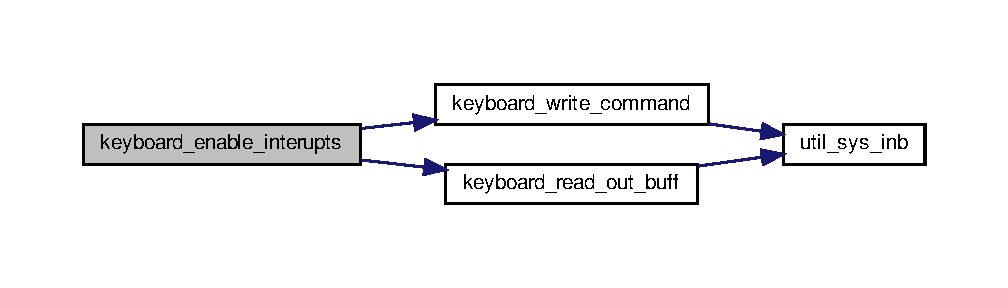
\includegraphics[width=350pt]{group__keyboard_ga0f2b9c07b7d16125c5fb2e05d9427e76_cgraph}
\end{center}
\end{figure}
\mbox{\Hypertarget{group__keyboard_gabb14446976ac2fcfaf095866f58d28ce}\label{group__keyboard_gabb14446976ac2fcfaf095866f58d28ce}} 
\index{keyboard@{keyboard}!keyboard\+\_\+\+IH@{keyboard\+\_\+\+IH}}
\index{keyboard\+\_\+\+IH@{keyboard\+\_\+\+IH}!keyboard@{keyboard}}
\subsubsection{\texorpdfstring{keyboard\+\_\+\+I\+H()}{keyboard\_IH()}}
{\footnotesize\ttfamily void() keyboard\+\_\+\+IH (\begin{DoxyParamCaption}{ }\end{DoxyParamCaption})}



Keyboard interupt handler. 

Here is the call graph for this function\+:\nopagebreak
\begin{figure}[H]
\begin{center}
\leavevmode
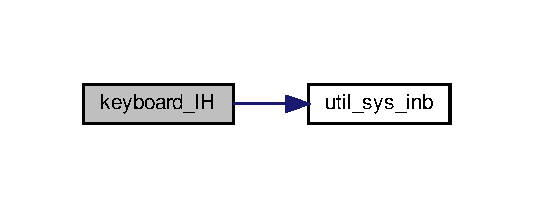
\includegraphics[width=256pt]{group__keyboard_gabb14446976ac2fcfaf095866f58d28ce_cgraph}
\end{center}
\end{figure}
Here is the caller graph for this function\+:\nopagebreak
\begin{figure}[H]
\begin{center}
\leavevmode
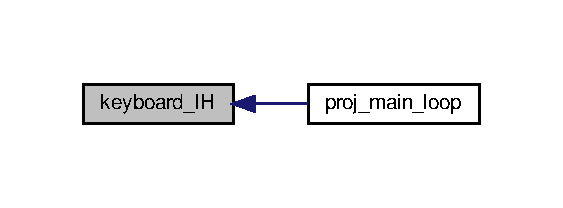
\includegraphics[width=270pt]{group__keyboard_gabb14446976ac2fcfaf095866f58d28ce_icgraph}
\end{center}
\end{figure}
\mbox{\Hypertarget{group__keyboard_ga01f4a2303581946d7d26fdb5ac7c0caf}\label{group__keyboard_ga01f4a2303581946d7d26fdb5ac7c0caf}} 
\index{keyboard@{keyboard}!keyboard\+\_\+read\+\_\+out\+\_\+buff@{keyboard\+\_\+read\+\_\+out\+\_\+buff}}
\index{keyboard\+\_\+read\+\_\+out\+\_\+buff@{keyboard\+\_\+read\+\_\+out\+\_\+buff}!keyboard@{keyboard}}
\subsubsection{\texorpdfstring{keyboard\+\_\+read\+\_\+out\+\_\+buff()}{keyboard\_read\_out\_buff()}}
{\footnotesize\ttfamily int() keyboard\+\_\+read\+\_\+out\+\_\+buff (\begin{DoxyParamCaption}\item[{uint8\+\_\+t $\ast$}]{output }\end{DoxyParamCaption})}



Reads from the out buffer. 

Here is the call graph for this function\+:\nopagebreak
\begin{figure}[H]
\begin{center}
\leavevmode
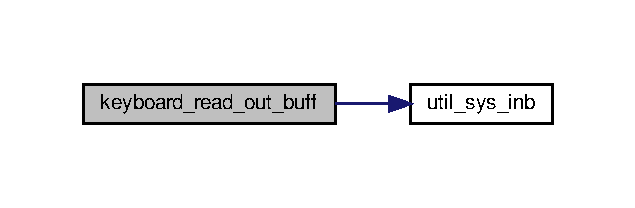
\includegraphics[width=305pt]{group__keyboard_ga01f4a2303581946d7d26fdb5ac7c0caf_cgraph}
\end{center}
\end{figure}
Here is the caller graph for this function\+:\nopagebreak
\begin{figure}[H]
\begin{center}
\leavevmode
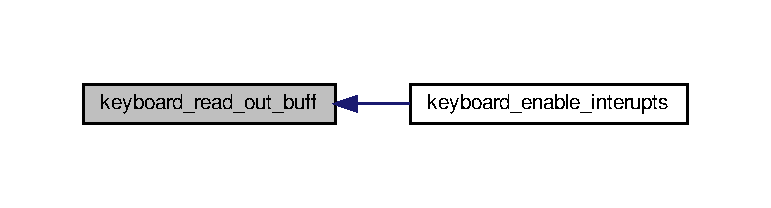
\includegraphics[width=350pt]{group__keyboard_ga01f4a2303581946d7d26fdb5ac7c0caf_icgraph}
\end{center}
\end{figure}
\mbox{\Hypertarget{group__keyboard_gaefd0e3aafc75eb71df4d778f356b6dd7}\label{group__keyboard_gaefd0e3aafc75eb71df4d778f356b6dd7}} 
\index{keyboard@{keyboard}!keyboard\+\_\+subscribe\+\_\+int@{keyboard\+\_\+subscribe\+\_\+int}}
\index{keyboard\+\_\+subscribe\+\_\+int@{keyboard\+\_\+subscribe\+\_\+int}!keyboard@{keyboard}}
\subsubsection{\texorpdfstring{keyboard\+\_\+subscribe\+\_\+int()}{keyboard\_subscribe\_int()}}
{\footnotesize\ttfamily int() keyboard\+\_\+subscribe\+\_\+int (\begin{DoxyParamCaption}\item[{int $\ast$}]{irq\+\_\+set }\end{DoxyParamCaption})}



Subscribe for keyboard interupts. 

Here is the caller graph for this function\+:\nopagebreak
\begin{figure}[H]
\begin{center}
\leavevmode
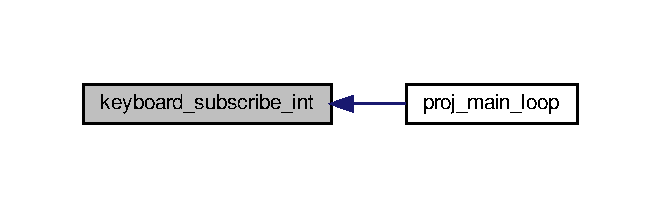
\includegraphics[width=317pt]{group__keyboard_gaefd0e3aafc75eb71df4d778f356b6dd7_icgraph}
\end{center}
\end{figure}
\mbox{\Hypertarget{group__keyboard_ga32cc4de66854f8a7bd909e7aa8b901ed}\label{group__keyboard_ga32cc4de66854f8a7bd909e7aa8b901ed}} 
\index{keyboard@{keyboard}!keyboard\+\_\+unsubscribe\+\_\+int@{keyboard\+\_\+unsubscribe\+\_\+int}}
\index{keyboard\+\_\+unsubscribe\+\_\+int@{keyboard\+\_\+unsubscribe\+\_\+int}!keyboard@{keyboard}}
\subsubsection{\texorpdfstring{keyboard\+\_\+unsubscribe\+\_\+int()}{keyboard\_unsubscribe\_int()}}
{\footnotesize\ttfamily int() keyboard\+\_\+unsubscribe\+\_\+int (\begin{DoxyParamCaption}{ }\end{DoxyParamCaption})}



Unsubscribe from keyboard interupts. 

Here is the caller graph for this function\+:\nopagebreak
\begin{figure}[H]
\begin{center}
\leavevmode
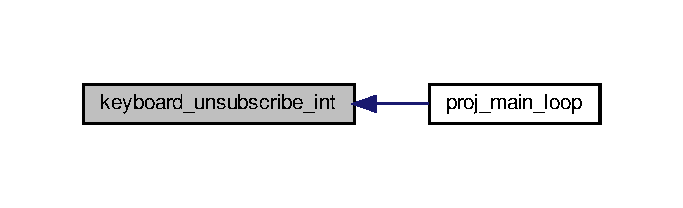
\includegraphics[width=328pt]{group__keyboard_ga32cc4de66854f8a7bd909e7aa8b901ed_icgraph}
\end{center}
\end{figure}
\mbox{\Hypertarget{group__keyboard_gad6f191b6116f8df3e057322f0c76b66a}\label{group__keyboard_gad6f191b6116f8df3e057322f0c76b66a}} 
\index{keyboard@{keyboard}!keyboard\+\_\+write\+\_\+command@{keyboard\+\_\+write\+\_\+command}}
\index{keyboard\+\_\+write\+\_\+command@{keyboard\+\_\+write\+\_\+command}!keyboard@{keyboard}}
\subsubsection{\texorpdfstring{keyboard\+\_\+write\+\_\+command()}{keyboard\_write\_command()}}
{\footnotesize\ttfamily int() keyboard\+\_\+write\+\_\+command (\begin{DoxyParamCaption}\item[{uint8\+\_\+t}]{reg,  }\item[{uint32\+\_\+t}]{cmd }\end{DoxyParamCaption})}



Write comand to register. 

Here is the call graph for this function\+:\nopagebreak
\begin{figure}[H]
\begin{center}
\leavevmode
\includegraphics[width=315pt]{group__keyboard_gad6f191b6116f8df3e057322f0c76b66a_cgraph}
\end{center}
\end{figure}
Here is the caller graph for this function\+:\nopagebreak
\begin{figure}[H]
\begin{center}
\leavevmode
\includegraphics[width=350pt]{group__keyboard_gad6f191b6116f8df3e057322f0c76b66a_icgraph}
\end{center}
\end{figure}
\mbox{\Hypertarget{group__keyboard_ga50ccd1d4a10b2f8d6f380d3581eae423}\label{group__keyboard_ga50ccd1d4a10b2f8d6f380d3581eae423}} 
\index{keyboard@{keyboard}!print\+\_\+scancode@{print\+\_\+scancode}}
\index{print\+\_\+scancode@{print\+\_\+scancode}!keyboard@{keyboard}}
\subsubsection{\texorpdfstring{print\+\_\+scancode()}{print\_scancode()}}
{\footnotesize\ttfamily int() print\+\_\+scancode (\begin{DoxyParamCaption}{ }\end{DoxyParamCaption})}



Prints scancode. 



\subsection{Variable Documentation}
\mbox{\Hypertarget{group__keyboard_ga325819a8e492ac69542e8b31705af6e9}\label{group__keyboard_ga325819a8e492ac69542e8b31705af6e9}} 
\index{keyboard@{keyboard}!data@{data}}
\index{data@{data}!keyboard@{keyboard}}
\subsubsection{\texorpdfstring{data}{data}}
{\footnotesize\ttfamily uint8\+\_\+t data}



Break code. 

\mbox{\Hypertarget{group__keyboard_ga1fab7e7fd2c88555db9e3dd5c3654ad3}\label{group__keyboard_ga1fab7e7fd2c88555db9e3dd5c3654ad3}} 
\index{keyboard@{keyboard}!data2byte@{data2byte}}
\index{data2byte@{data2byte}!keyboard@{keyboard}}
\subsubsection{\texorpdfstring{data2byte}{data2byte}}
{\footnotesize\ttfamily uint8\+\_\+t data2byte\mbox{[}2\mbox{]}}



Keyboard data for the case the scancode is 2 byte long. 

\mbox{\Hypertarget{group__keyboard_ga7276dae9c8b623a99137f24b3b6b549e}\label{group__keyboard_ga7276dae9c8b623a99137f24b3b6b549e}} 
\index{keyboard@{keyboard}!is\+\_\+2\+\_\+byte@{is\+\_\+2\+\_\+byte}}
\index{is\+\_\+2\+\_\+byte@{is\+\_\+2\+\_\+byte}!keyboard@{keyboard}}
\subsubsection{\texorpdfstring{is\+\_\+2\+\_\+byte}{is\_2\_byte}}
{\footnotesize\ttfamily bool is\+\_\+2\+\_\+byte = false}



If the code is 2 byte long. 

\mbox{\Hypertarget{group__keyboard_ga74708534432e98d4ab30ba40e2e5dcc3}\label{group__keyboard_ga74708534432e98d4ab30ba40e2e5dcc3}} 
\index{keyboard@{keyboard}!kbd\+\_\+hook\+\_\+id@{kbd\+\_\+hook\+\_\+id}}
\index{kbd\+\_\+hook\+\_\+id@{kbd\+\_\+hook\+\_\+id}!keyboard@{keyboard}}
\subsubsection{\texorpdfstring{kbd\+\_\+hook\+\_\+id}{kbd\_hook\_id}}
{\footnotesize\ttfamily int kbd\+\_\+hook\+\_\+id = 1}



Keyboard hook id. 

\mbox{\Hypertarget{group__keyboard_ga96f7c2f0fe863bd78294a8f639e60478}\label{group__keyboard_ga96f7c2f0fe863bd78294a8f639e60478}} 
\index{keyboard@{keyboard}!new\+\_\+scancode@{new\+\_\+scancode}}
\index{new\+\_\+scancode@{new\+\_\+scancode}!keyboard@{keyboard}}
\subsubsection{\texorpdfstring{new\+\_\+scancode}{new\_scancode}}
{\footnotesize\ttfamily bool new\+\_\+scancode = false}



If the scancode recived is new or not. 


\hypertarget{group__Main-Menu}{}\section{Main-\/\+Menu}
\label{group__Main-Menu}\index{Main-\/\+Menu@{Main-\/\+Menu}}
\subsection*{Functions}
\begin{DoxyCompactItemize}
\item 
void \hyperlink{group__Main-Menu_ga26d3dd4d93472051b4e0bb50e319494b}{load\+\_\+sprites} ()
\begin{DoxyCompactList}\small\item\em Loads the X\+PM into xpm\+\_\+image\+\_\+t for further use. \end{DoxyCompactList}\item 
void \hyperlink{group__Main-Menu_gab084ce5f50d30f5b66396d4afa61f3a0}{main\+\_\+menu\+\_\+frame} ()
\begin{DoxyCompactList}\small\item\em Called once per frame on main menu. \end{DoxyCompactList}\item 
void \hyperlink{group__Main-Menu_gaa455d5f53d6465e1e8c467bbc1231f47}{main\+\_\+menu\+\_\+keyboard} (uint8\+\_\+t \hyperlink{group__Proj_ga325819a8e492ac69542e8b31705af6e9}{data})
\begin{DoxyCompactList}\small\item\em Called once per keyboard interupt, manages exit. \end{DoxyCompactList}\item 
void \hyperlink{group__Main-Menu_ga4a8e0e77f8775d3742bbda1b8c48fd3c}{main\+\_\+menu\+\_\+mouse} (struct packet pckt)
\begin{DoxyCompactList}\small\item\em Called once per mouse interupt, manages mouse position and click. \end{DoxyCompactList}\end{DoxyCompactItemize}
\subsection*{Variables}
\begin{DoxyCompactItemize}
\item 
enum \hyperlink{group__utils_gad0ed1832dd134806ad335cdcc1a59ad2}{game\+\_\+state} \hyperlink{group__Main-Menu_ga38caf7c28534bcd60ff95faf7fcae2d7}{game\+\_\+state}
\begin{DoxyCompactList}\small\item\em Current game state. \end{DoxyCompactList}\item 
int \hyperlink{group__Main-Menu_ga6c59af730728bf5260ef828aea2eebee}{mouse\+\_\+x} = \hyperlink{group__utils_ga2cd109632a6dcccaa80b43561b1ab700}{S\+C\+R\+E\+E\+N\+\_\+\+W\+I\+D\+TH}/2
\begin{DoxyCompactList}\small\item\em Mouse x position. \end{DoxyCompactList}\item 
int \hyperlink{group__Main-Menu_gab21653e455bbca86826aa5f628a5fdb2}{mouse\+\_\+y} = \hyperlink{group__utils_ga6974d08a74da681b3957b2fead2608b8}{S\+C\+R\+E\+E\+N\+\_\+\+H\+E\+I\+G\+HT}/2
\begin{DoxyCompactList}\small\item\em Mouse y position. \end{DoxyCompactList}\item 
int \hyperlink{group__Main-Menu_gad7f272c01893c7161961744eb23516d0}{o\+\_\+mouse\+\_\+x} = 0
\begin{DoxyCompactList}\small\item\em Mouse x position in last frame. \end{DoxyCompactList}\item 
int \hyperlink{group__Main-Menu_ga7c7344b212ca479c18185090a37e0d29}{o\+\_\+mouse\+\_\+y} = 0
\begin{DoxyCompactList}\small\item\em Mouse y position in last frame. \end{DoxyCompactList}\item 
xpm\+\_\+image\+\_\+t \hyperlink{group__Main-Menu_ga1713b7f6ecba05ea9e8281f216eb8818}{mouse\+\_\+sprite}
\begin{DoxyCompactList}\small\item\em Mouse cursor sprite. \end{DoxyCompactList}\item 
xpm\+\_\+image\+\_\+t \hyperlink{group__Main-Menu_ga69acbc91c439d0d9f047cbe70ade84cc}{alien\+\_\+sprite}
\begin{DoxyCompactList}\small\item\em Alien player sprite. \end{DoxyCompactList}\item 
xpm\+\_\+image\+\_\+t \hyperlink{group__Main-Menu_ga45f80f61d0103ffc208c2d0493380fb2}{asteroid\+\_\+sprite}
\begin{DoxyCompactList}\small\item\em Asteroid sprite. \end{DoxyCompactList}\item 
xpm\+\_\+image\+\_\+t \hyperlink{group__Main-Menu_ga06a70f098733d826cb9d8e81e7104983}{broken\+\_\+asteroid\+\_\+sprite}
\begin{DoxyCompactList}\small\item\em Broken asteroid sprite. \end{DoxyCompactList}\item 
xpm\+\_\+image\+\_\+t \hyperlink{group__Main-Menu_ga5a4cfb92e48a82e5d50c87e4bc632970}{background\+\_\+sprite}
\begin{DoxyCompactList}\small\item\em Background sprite. \end{DoxyCompactList}\item 
xpm\+\_\+image\+\_\+t \hyperlink{group__Main-Menu_ga55fa0635c490a8f9333972d949a5216e}{title\+\_\+sprite}
\begin{DoxyCompactList}\small\item\em Title name sprite. \end{DoxyCompactList}\item 
xpm\+\_\+image\+\_\+t \hyperlink{group__Main-Menu_ga5bb71c838fd9ce7847f379d2c17483ab}{how\+\_\+to\+\_\+play\+\_\+sprite}
\begin{DoxyCompactList}\small\item\em How to play text sprite. \end{DoxyCompactList}\item 
xpm\+\_\+image\+\_\+t \hyperlink{group__Main-Menu_ga522a4ef9103746c5c1ba61e915e39f0a}{start\+\_\+sprite}
\begin{DoxyCompactList}\small\item\em Start button sprite. \end{DoxyCompactList}\item 
xpm\+\_\+image\+\_\+t \hyperlink{group__Main-Menu_ga151ed16274d40549e8aa6715aa4c715a}{exit\+\_\+sprite}
\begin{DoxyCompactList}\small\item\em Exit button sprite. \end{DoxyCompactList}\item 
xpm\+\_\+image\+\_\+t \hyperlink{group__Main-Menu_ga75a1070484069c0a4b134cb82e89285f}{game\+\_\+over\+\_\+sprite}
\begin{DoxyCompactList}\small\item\em Game over text sprite. \end{DoxyCompactList}\item 
xpm\+\_\+image\+\_\+t \hyperlink{group__Main-Menu_ga9c8097218050947104e9eff7ea72ee2a}{score\+\_\+sprite}
\begin{DoxyCompactList}\small\item\em Score text sprite. \end{DoxyCompactList}\item 
xpm\+\_\+image\+\_\+t \hyperlink{group__Main-Menu_gaa41380dca9e42a7214c4383a057eb1b5}{try\+\_\+again\+\_\+sprite}
\begin{DoxyCompactList}\small\item\em try again button sprite \end{DoxyCompactList}\item 
xpm\+\_\+image\+\_\+t \hyperlink{group__Main-Menu_ga4e9f74a7ebd652ff9289c657ccbcbad2}{score\+\_\+board\+\_\+sprite}
\begin{DoxyCompactList}\small\item\em score board button sprite \end{DoxyCompactList}\item 
xpm\+\_\+image\+\_\+t \hyperlink{group__Main-Menu_ga6e4a5f1f16e719a78ad8112fba87dc55}{top10\+\_\+sprite}
\begin{DoxyCompactList}\small\item\em top 10 text sprite \end{DoxyCompactList}\item 
xpm\+\_\+image\+\_\+t \hyperlink{group__Main-Menu_ga794827f066c5e8fa039cae3a45f7b2c0}{title\+\_\+screen\+\_\+sprite}
\begin{DoxyCompactList}\small\item\em title screen button sprite \end{DoxyCompactList}\end{DoxyCompactItemize}


\subsection{Detailed Description}
Contais tha code for the main menu screen 

\subsection{Function Documentation}
\mbox{\Hypertarget{group__Main-Menu_ga26d3dd4d93472051b4e0bb50e319494b}\label{group__Main-Menu_ga26d3dd4d93472051b4e0bb50e319494b}} 
\index{Main-\/\+Menu@{Main-\/\+Menu}!load\+\_\+sprites@{load\+\_\+sprites}}
\index{load\+\_\+sprites@{load\+\_\+sprites}!Main-\/\+Menu@{Main-\/\+Menu}}
\subsubsection{\texorpdfstring{load\+\_\+sprites()}{load\_sprites()}}
{\footnotesize\ttfamily void load\+\_\+sprites (\begin{DoxyParamCaption}{ }\end{DoxyParamCaption})}



Loads the X\+PM into xpm\+\_\+image\+\_\+t for further use. 

Here is the call graph for this function\+:\nopagebreak
\begin{figure}[H]
\begin{center}
\leavevmode
\includegraphics[width=350pt]{group__Main-Menu_ga26d3dd4d93472051b4e0bb50e319494b_cgraph}
\end{center}
\end{figure}
Here is the caller graph for this function\+:\nopagebreak
\begin{figure}[H]
\begin{center}
\leavevmode
\includegraphics[width=267pt]{group__Main-Menu_ga26d3dd4d93472051b4e0bb50e319494b_icgraph}
\end{center}
\end{figure}
\mbox{\Hypertarget{group__Main-Menu_gab084ce5f50d30f5b66396d4afa61f3a0}\label{group__Main-Menu_gab084ce5f50d30f5b66396d4afa61f3a0}} 
\index{Main-\/\+Menu@{Main-\/\+Menu}!main\+\_\+menu\+\_\+frame@{main\+\_\+menu\+\_\+frame}}
\index{main\+\_\+menu\+\_\+frame@{main\+\_\+menu\+\_\+frame}!Main-\/\+Menu@{Main-\/\+Menu}}
\subsubsection{\texorpdfstring{main\+\_\+menu\+\_\+frame()}{main\_menu\_frame()}}
{\footnotesize\ttfamily void main\+\_\+menu\+\_\+frame (\begin{DoxyParamCaption}{ }\end{DoxyParamCaption})}



Called once per frame on main menu. 

Here is the call graph for this function\+:\nopagebreak
\begin{figure}[H]
\begin{center}
\leavevmode
\includegraphics[width=350pt]{group__Main-Menu_gab084ce5f50d30f5b66396d4afa61f3a0_cgraph}
\end{center}
\end{figure}
Here is the caller graph for this function\+:\nopagebreak
\begin{figure}[H]
\begin{center}
\leavevmode
\includegraphics[width=295pt]{group__Main-Menu_gab084ce5f50d30f5b66396d4afa61f3a0_icgraph}
\end{center}
\end{figure}
\mbox{\Hypertarget{group__Main-Menu_gaa455d5f53d6465e1e8c467bbc1231f47}\label{group__Main-Menu_gaa455d5f53d6465e1e8c467bbc1231f47}} 
\index{Main-\/\+Menu@{Main-\/\+Menu}!main\+\_\+menu\+\_\+keyboard@{main\+\_\+menu\+\_\+keyboard}}
\index{main\+\_\+menu\+\_\+keyboard@{main\+\_\+menu\+\_\+keyboard}!Main-\/\+Menu@{Main-\/\+Menu}}
\subsubsection{\texorpdfstring{main\+\_\+menu\+\_\+keyboard()}{main\_menu\_keyboard()}}
{\footnotesize\ttfamily void main\+\_\+menu\+\_\+keyboard (\begin{DoxyParamCaption}\item[{uint8\+\_\+t}]{data }\end{DoxyParamCaption})}



Called once per keyboard interupt, manages exit. 

Here is the call graph for this function\+:\nopagebreak
\begin{figure}[H]
\begin{center}
\leavevmode
\includegraphics[width=350pt]{group__Main-Menu_gaa455d5f53d6465e1e8c467bbc1231f47_cgraph}
\end{center}
\end{figure}
Here is the caller graph for this function\+:\nopagebreak
\begin{figure}[H]
\begin{center}
\leavevmode
\includegraphics[width=310pt]{group__Main-Menu_gaa455d5f53d6465e1e8c467bbc1231f47_icgraph}
\end{center}
\end{figure}
\mbox{\Hypertarget{group__Main-Menu_ga4a8e0e77f8775d3742bbda1b8c48fd3c}\label{group__Main-Menu_ga4a8e0e77f8775d3742bbda1b8c48fd3c}} 
\index{Main-\/\+Menu@{Main-\/\+Menu}!main\+\_\+menu\+\_\+mouse@{main\+\_\+menu\+\_\+mouse}}
\index{main\+\_\+menu\+\_\+mouse@{main\+\_\+menu\+\_\+mouse}!Main-\/\+Menu@{Main-\/\+Menu}}
\subsubsection{\texorpdfstring{main\+\_\+menu\+\_\+mouse()}{main\_menu\_mouse()}}
{\footnotesize\ttfamily void main\+\_\+menu\+\_\+mouse (\begin{DoxyParamCaption}\item[{struct packet}]{pckt }\end{DoxyParamCaption})}



Called once per mouse interupt, manages mouse position and click. 

Here is the call graph for this function\+:\nopagebreak
\begin{figure}[H]
\begin{center}
\leavevmode
\includegraphics[width=350pt]{group__Main-Menu_ga4a8e0e77f8775d3742bbda1b8c48fd3c_cgraph}
\end{center}
\end{figure}
Here is the caller graph for this function\+:\nopagebreak
\begin{figure}[H]
\begin{center}
\leavevmode
\includegraphics[width=299pt]{group__Main-Menu_ga4a8e0e77f8775d3742bbda1b8c48fd3c_icgraph}
\end{center}
\end{figure}


\subsection{Variable Documentation}
\mbox{\Hypertarget{group__Main-Menu_ga69acbc91c439d0d9f047cbe70ade84cc}\label{group__Main-Menu_ga69acbc91c439d0d9f047cbe70ade84cc}} 
\index{Main-\/\+Menu@{Main-\/\+Menu}!alien\+\_\+sprite@{alien\+\_\+sprite}}
\index{alien\+\_\+sprite@{alien\+\_\+sprite}!Main-\/\+Menu@{Main-\/\+Menu}}
\subsubsection{\texorpdfstring{alien\+\_\+sprite}{alien\_sprite}}
{\footnotesize\ttfamily xpm\+\_\+image\+\_\+t alien\+\_\+sprite}



Alien player sprite. 

\mbox{\Hypertarget{group__Main-Menu_ga45f80f61d0103ffc208c2d0493380fb2}\label{group__Main-Menu_ga45f80f61d0103ffc208c2d0493380fb2}} 
\index{Main-\/\+Menu@{Main-\/\+Menu}!asteroid\+\_\+sprite@{asteroid\+\_\+sprite}}
\index{asteroid\+\_\+sprite@{asteroid\+\_\+sprite}!Main-\/\+Menu@{Main-\/\+Menu}}
\subsubsection{\texorpdfstring{asteroid\+\_\+sprite}{asteroid\_sprite}}
{\footnotesize\ttfamily xpm\+\_\+image\+\_\+t asteroid\+\_\+sprite}



Asteroid sprite. 

\mbox{\Hypertarget{group__Main-Menu_ga5a4cfb92e48a82e5d50c87e4bc632970}\label{group__Main-Menu_ga5a4cfb92e48a82e5d50c87e4bc632970}} 
\index{Main-\/\+Menu@{Main-\/\+Menu}!background\+\_\+sprite@{background\+\_\+sprite}}
\index{background\+\_\+sprite@{background\+\_\+sprite}!Main-\/\+Menu@{Main-\/\+Menu}}
\subsubsection{\texorpdfstring{background\+\_\+sprite}{background\_sprite}}
{\footnotesize\ttfamily xpm\+\_\+image\+\_\+t background\+\_\+sprite}



Background sprite. 

\mbox{\Hypertarget{group__Main-Menu_ga06a70f098733d826cb9d8e81e7104983}\label{group__Main-Menu_ga06a70f098733d826cb9d8e81e7104983}} 
\index{Main-\/\+Menu@{Main-\/\+Menu}!broken\+\_\+asteroid\+\_\+sprite@{broken\+\_\+asteroid\+\_\+sprite}}
\index{broken\+\_\+asteroid\+\_\+sprite@{broken\+\_\+asteroid\+\_\+sprite}!Main-\/\+Menu@{Main-\/\+Menu}}
\subsubsection{\texorpdfstring{broken\+\_\+asteroid\+\_\+sprite}{broken\_asteroid\_sprite}}
{\footnotesize\ttfamily xpm\+\_\+image\+\_\+t broken\+\_\+asteroid\+\_\+sprite}



Broken asteroid sprite. 

\mbox{\Hypertarget{group__Main-Menu_ga151ed16274d40549e8aa6715aa4c715a}\label{group__Main-Menu_ga151ed16274d40549e8aa6715aa4c715a}} 
\index{Main-\/\+Menu@{Main-\/\+Menu}!exit\+\_\+sprite@{exit\+\_\+sprite}}
\index{exit\+\_\+sprite@{exit\+\_\+sprite}!Main-\/\+Menu@{Main-\/\+Menu}}
\subsubsection{\texorpdfstring{exit\+\_\+sprite}{exit\_sprite}}
{\footnotesize\ttfamily xpm\+\_\+image\+\_\+t exit\+\_\+sprite}



Exit button sprite. 

\mbox{\Hypertarget{group__Main-Menu_ga75a1070484069c0a4b134cb82e89285f}\label{group__Main-Menu_ga75a1070484069c0a4b134cb82e89285f}} 
\index{Main-\/\+Menu@{Main-\/\+Menu}!game\+\_\+over\+\_\+sprite@{game\+\_\+over\+\_\+sprite}}
\index{game\+\_\+over\+\_\+sprite@{game\+\_\+over\+\_\+sprite}!Main-\/\+Menu@{Main-\/\+Menu}}
\subsubsection{\texorpdfstring{game\+\_\+over\+\_\+sprite}{game\_over\_sprite}}
{\footnotesize\ttfamily xpm\+\_\+image\+\_\+t game\+\_\+over\+\_\+sprite}



Game over text sprite. 

\mbox{\Hypertarget{group__Main-Menu_ga38caf7c28534bcd60ff95faf7fcae2d7}\label{group__Main-Menu_ga38caf7c28534bcd60ff95faf7fcae2d7}} 
\index{Main-\/\+Menu@{Main-\/\+Menu}!game\+\_\+state@{game\+\_\+state}}
\index{game\+\_\+state@{game\+\_\+state}!Main-\/\+Menu@{Main-\/\+Menu}}
\subsubsection{\texorpdfstring{game\+\_\+state}{game\_state}}
{\footnotesize\ttfamily enum \hyperlink{group__utils_gad0ed1832dd134806ad335cdcc1a59ad2}{game\+\_\+state} \hyperlink{group__utils_gad0ed1832dd134806ad335cdcc1a59ad2}{game\+\_\+state}}



Current game state. 

\mbox{\Hypertarget{group__Main-Menu_ga5bb71c838fd9ce7847f379d2c17483ab}\label{group__Main-Menu_ga5bb71c838fd9ce7847f379d2c17483ab}} 
\index{Main-\/\+Menu@{Main-\/\+Menu}!how\+\_\+to\+\_\+play\+\_\+sprite@{how\+\_\+to\+\_\+play\+\_\+sprite}}
\index{how\+\_\+to\+\_\+play\+\_\+sprite@{how\+\_\+to\+\_\+play\+\_\+sprite}!Main-\/\+Menu@{Main-\/\+Menu}}
\subsubsection{\texorpdfstring{how\+\_\+to\+\_\+play\+\_\+sprite}{how\_to\_play\_sprite}}
{\footnotesize\ttfamily xpm\+\_\+image\+\_\+t how\+\_\+to\+\_\+play\+\_\+sprite}



How to play text sprite. 

\mbox{\Hypertarget{group__Main-Menu_ga1713b7f6ecba05ea9e8281f216eb8818}\label{group__Main-Menu_ga1713b7f6ecba05ea9e8281f216eb8818}} 
\index{Main-\/\+Menu@{Main-\/\+Menu}!mouse\+\_\+sprite@{mouse\+\_\+sprite}}
\index{mouse\+\_\+sprite@{mouse\+\_\+sprite}!Main-\/\+Menu@{Main-\/\+Menu}}
\subsubsection{\texorpdfstring{mouse\+\_\+sprite}{mouse\_sprite}}
{\footnotesize\ttfamily xpm\+\_\+image\+\_\+t mouse\+\_\+sprite}



Mouse cursor sprite. 

\mbox{\Hypertarget{group__Main-Menu_ga6c59af730728bf5260ef828aea2eebee}\label{group__Main-Menu_ga6c59af730728bf5260ef828aea2eebee}} 
\index{Main-\/\+Menu@{Main-\/\+Menu}!mouse\+\_\+x@{mouse\+\_\+x}}
\index{mouse\+\_\+x@{mouse\+\_\+x}!Main-\/\+Menu@{Main-\/\+Menu}}
\subsubsection{\texorpdfstring{mouse\+\_\+x}{mouse\_x}}
{\footnotesize\ttfamily int mouse\+\_\+x = \hyperlink{group__utils_ga2cd109632a6dcccaa80b43561b1ab700}{S\+C\+R\+E\+E\+N\+\_\+\+W\+I\+D\+TH}/2}



Mouse x position. 

\mbox{\Hypertarget{group__Main-Menu_gab21653e455bbca86826aa5f628a5fdb2}\label{group__Main-Menu_gab21653e455bbca86826aa5f628a5fdb2}} 
\index{Main-\/\+Menu@{Main-\/\+Menu}!mouse\+\_\+y@{mouse\+\_\+y}}
\index{mouse\+\_\+y@{mouse\+\_\+y}!Main-\/\+Menu@{Main-\/\+Menu}}
\subsubsection{\texorpdfstring{mouse\+\_\+y}{mouse\_y}}
{\footnotesize\ttfamily int mouse\+\_\+y = \hyperlink{group__utils_ga6974d08a74da681b3957b2fead2608b8}{S\+C\+R\+E\+E\+N\+\_\+\+H\+E\+I\+G\+HT}/2}



Mouse y position. 

\mbox{\Hypertarget{group__Main-Menu_gad7f272c01893c7161961744eb23516d0}\label{group__Main-Menu_gad7f272c01893c7161961744eb23516d0}} 
\index{Main-\/\+Menu@{Main-\/\+Menu}!o\+\_\+mouse\+\_\+x@{o\+\_\+mouse\+\_\+x}}
\index{o\+\_\+mouse\+\_\+x@{o\+\_\+mouse\+\_\+x}!Main-\/\+Menu@{Main-\/\+Menu}}
\subsubsection{\texorpdfstring{o\+\_\+mouse\+\_\+x}{o\_mouse\_x}}
{\footnotesize\ttfamily int o\+\_\+mouse\+\_\+x = 0}



Mouse x position in last frame. 

\mbox{\Hypertarget{group__Main-Menu_ga7c7344b212ca479c18185090a37e0d29}\label{group__Main-Menu_ga7c7344b212ca479c18185090a37e0d29}} 
\index{Main-\/\+Menu@{Main-\/\+Menu}!o\+\_\+mouse\+\_\+y@{o\+\_\+mouse\+\_\+y}}
\index{o\+\_\+mouse\+\_\+y@{o\+\_\+mouse\+\_\+y}!Main-\/\+Menu@{Main-\/\+Menu}}
\subsubsection{\texorpdfstring{o\+\_\+mouse\+\_\+y}{o\_mouse\_y}}
{\footnotesize\ttfamily int o\+\_\+mouse\+\_\+y = 0}



Mouse y position in last frame. 

\mbox{\Hypertarget{group__Main-Menu_ga4e9f74a7ebd652ff9289c657ccbcbad2}\label{group__Main-Menu_ga4e9f74a7ebd652ff9289c657ccbcbad2}} 
\index{Main-\/\+Menu@{Main-\/\+Menu}!score\+\_\+board\+\_\+sprite@{score\+\_\+board\+\_\+sprite}}
\index{score\+\_\+board\+\_\+sprite@{score\+\_\+board\+\_\+sprite}!Main-\/\+Menu@{Main-\/\+Menu}}
\subsubsection{\texorpdfstring{score\+\_\+board\+\_\+sprite}{score\_board\_sprite}}
{\footnotesize\ttfamily xpm\+\_\+image\+\_\+t score\+\_\+board\+\_\+sprite}



score board button sprite 

\mbox{\Hypertarget{group__Main-Menu_ga9c8097218050947104e9eff7ea72ee2a}\label{group__Main-Menu_ga9c8097218050947104e9eff7ea72ee2a}} 
\index{Main-\/\+Menu@{Main-\/\+Menu}!score\+\_\+sprite@{score\+\_\+sprite}}
\index{score\+\_\+sprite@{score\+\_\+sprite}!Main-\/\+Menu@{Main-\/\+Menu}}
\subsubsection{\texorpdfstring{score\+\_\+sprite}{score\_sprite}}
{\footnotesize\ttfamily xpm\+\_\+image\+\_\+t score\+\_\+sprite}



Score text sprite. 

\mbox{\Hypertarget{group__Main-Menu_ga522a4ef9103746c5c1ba61e915e39f0a}\label{group__Main-Menu_ga522a4ef9103746c5c1ba61e915e39f0a}} 
\index{Main-\/\+Menu@{Main-\/\+Menu}!start\+\_\+sprite@{start\+\_\+sprite}}
\index{start\+\_\+sprite@{start\+\_\+sprite}!Main-\/\+Menu@{Main-\/\+Menu}}
\subsubsection{\texorpdfstring{start\+\_\+sprite}{start\_sprite}}
{\footnotesize\ttfamily xpm\+\_\+image\+\_\+t start\+\_\+sprite}



Start button sprite. 

\mbox{\Hypertarget{group__Main-Menu_ga794827f066c5e8fa039cae3a45f7b2c0}\label{group__Main-Menu_ga794827f066c5e8fa039cae3a45f7b2c0}} 
\index{Main-\/\+Menu@{Main-\/\+Menu}!title\+\_\+screen\+\_\+sprite@{title\+\_\+screen\+\_\+sprite}}
\index{title\+\_\+screen\+\_\+sprite@{title\+\_\+screen\+\_\+sprite}!Main-\/\+Menu@{Main-\/\+Menu}}
\subsubsection{\texorpdfstring{title\+\_\+screen\+\_\+sprite}{title\_screen\_sprite}}
{\footnotesize\ttfamily xpm\+\_\+image\+\_\+t title\+\_\+screen\+\_\+sprite}



title screen button sprite 

\mbox{\Hypertarget{group__Main-Menu_ga55fa0635c490a8f9333972d949a5216e}\label{group__Main-Menu_ga55fa0635c490a8f9333972d949a5216e}} 
\index{Main-\/\+Menu@{Main-\/\+Menu}!title\+\_\+sprite@{title\+\_\+sprite}}
\index{title\+\_\+sprite@{title\+\_\+sprite}!Main-\/\+Menu@{Main-\/\+Menu}}
\subsubsection{\texorpdfstring{title\+\_\+sprite}{title\_sprite}}
{\footnotesize\ttfamily xpm\+\_\+image\+\_\+t title\+\_\+sprite}



Title name sprite. 

\mbox{\Hypertarget{group__Main-Menu_ga6e4a5f1f16e719a78ad8112fba87dc55}\label{group__Main-Menu_ga6e4a5f1f16e719a78ad8112fba87dc55}} 
\index{Main-\/\+Menu@{Main-\/\+Menu}!top10\+\_\+sprite@{top10\+\_\+sprite}}
\index{top10\+\_\+sprite@{top10\+\_\+sprite}!Main-\/\+Menu@{Main-\/\+Menu}}
\subsubsection{\texorpdfstring{top10\+\_\+sprite}{top10\_sprite}}
{\footnotesize\ttfamily xpm\+\_\+image\+\_\+t top10\+\_\+sprite}



top 10 text sprite 

\mbox{\Hypertarget{group__Main-Menu_gaa41380dca9e42a7214c4383a057eb1b5}\label{group__Main-Menu_gaa41380dca9e42a7214c4383a057eb1b5}} 
\index{Main-\/\+Menu@{Main-\/\+Menu}!try\+\_\+again\+\_\+sprite@{try\+\_\+again\+\_\+sprite}}
\index{try\+\_\+again\+\_\+sprite@{try\+\_\+again\+\_\+sprite}!Main-\/\+Menu@{Main-\/\+Menu}}
\subsubsection{\texorpdfstring{try\+\_\+again\+\_\+sprite}{try\_again\_sprite}}
{\footnotesize\ttfamily xpm\+\_\+image\+\_\+t try\+\_\+again\+\_\+sprite}



try again button sprite 


\hypertarget{group__mouse}{}\section{mouse}
\label{group__mouse}\index{mouse@{mouse}}
\subsection*{Functions}
\begin{DoxyCompactItemize}
\item 
int() \hyperlink{group__mouse_gaf55e4d1ccae1ac1f59dfa4222fd5de8e}{mouse\+\_\+subscribe\+\_\+int} (int $\ast$irq\+\_\+set)
\item 
int() \hyperlink{group__mouse_ga3ecf823d80520009ae5e0d76ae40a3c3}{mouse\+\_\+unsubscribe\+\_\+int} ()
\item 
int() \hyperlink{group__mouse_ga8931196769eb020bd34b8b93ee8c1ef6}{set\+Mouse\+I\+RQ} (bool enable)
\item 
int() \hyperlink{group__mouse_ga090c9bebd05709adc5de77ab5b26d7c3}{mouse\+\_\+write\+\_\+command} (uint8\+\_\+t cmd)
\item 
void() \hyperlink{group__mouse_ga210374b50462acdedab00df64d5cea3c}{mouse\+\_\+ih} ()
\item 
void() \hyperlink{group__mouse_ga3f43ee9f00f28eb503b80a8589216e5f}{mouse\+\_\+read\+\_\+out\+\_\+buff} ()
\item 
void() \hyperlink{group__mouse_ga025476b3734400554e7ead9c841b9ed9}{state\+\_\+machine} (struct packet $\ast$pckt, uint8\+\_\+t x\+\_\+len, uint8\+\_\+t tolerance)
\item 
int() \hyperlink{group__mouse_gabd35692be21807c9d3f1ae016fe7d6ec}{create\+Mouse\+Packet} (struct packet $\ast$pckt, uint8\+\_\+t data3byte\mbox{[}$\,$\mbox{]})
\item 
int() \hyperlink{group__mouse_gae5083fea5f4e764204c98e646ac25cc6}{set\+\_\+kbc\+\_\+cmd\+\_\+byte\+\_\+dflt} ()
\end{DoxyCompactItemize}
\subsection*{Variables}
\begin{DoxyCompactItemize}
\item 
int \hyperlink{group__mouse_ga37cad7cad93664f8a1ed1b0258fe958b}{mouse\+\_\+hook\+\_\+id} = 2
\item 
uint8\+\_\+t \hyperlink{group__mouse_ga325819a8e492ac69542e8b31705af6e9}{data}
\begin{DoxyCompactList}\small\item\em Break code. \end{DoxyCompactList}\item 
uint8\+\_\+t \hyperlink{group__mouse_ga9f33ecfca24a9211fc0fe7d4633087be}{data3bytes} \mbox{[}3\mbox{]}
\item 
int \hyperlink{group__mouse_ga33c33c30bb98b3e86f856cc0f031d1f2}{delta\+\_\+x} = 0
\item 
int \hyperlink{group__mouse_ga293bf93983300c292a4aaa40d7104917}{delta\+\_\+y} = 0
\item 
\hyperlink{mouse_8h_aa0aafed44fec19806d8f9ad834be1248}{state\+\_\+t} \hyperlink{group__mouse_ga9a379079ab305d43e4c73334578f9325}{st} = \hyperlink{mouse_8h_aa0aafed44fec19806d8f9ad834be1248a0cb1b2c6a7db1f1084886c98909a3f36}{I\+N\+IT}
\end{DoxyCompactItemize}


\subsection{Detailed Description}
Contais tha code to controll the mouse controller 

\subsection{Function Documentation}
\mbox{\Hypertarget{group__mouse_gabd35692be21807c9d3f1ae016fe7d6ec}\label{group__mouse_gabd35692be21807c9d3f1ae016fe7d6ec}} 
\index{mouse@{mouse}!create\+Mouse\+Packet@{create\+Mouse\+Packet}}
\index{create\+Mouse\+Packet@{create\+Mouse\+Packet}!mouse@{mouse}}
\subsubsection{\texorpdfstring{create\+Mouse\+Packet()}{createMousePacket()}}
{\footnotesize\ttfamily int() create\+Mouse\+Packet (\begin{DoxyParamCaption}\item[{struct packet $\ast$}]{pckt,  }\item[{uint8\+\_\+t}]{data3byte\mbox{[}$\,$\mbox{]} }\end{DoxyParamCaption})}

Here is the caller graph for this function\+:\nopagebreak
\begin{figure}[H]
\begin{center}
\leavevmode
\includegraphics[width=302pt]{group__mouse_gabd35692be21807c9d3f1ae016fe7d6ec_icgraph}
\end{center}
\end{figure}
\mbox{\Hypertarget{group__mouse_ga210374b50462acdedab00df64d5cea3c}\label{group__mouse_ga210374b50462acdedab00df64d5cea3c}} 
\index{mouse@{mouse}!mouse\+\_\+ih@{mouse\+\_\+ih}}
\index{mouse\+\_\+ih@{mouse\+\_\+ih}!mouse@{mouse}}
\subsubsection{\texorpdfstring{mouse\+\_\+ih()}{mouse\_ih()}}
{\footnotesize\ttfamily void() mouse\+\_\+ih (\begin{DoxyParamCaption}\item[{void}]{ }\end{DoxyParamCaption})}

Here is the call graph for this function\+:\nopagebreak
\begin{figure}[H]
\begin{center}
\leavevmode
\includegraphics[width=350pt]{group__mouse_ga210374b50462acdedab00df64d5cea3c_cgraph}
\end{center}
\end{figure}
Here is the caller graph for this function\+:\nopagebreak
\begin{figure}[H]
\begin{center}
\leavevmode
\includegraphics[width=257pt]{group__mouse_ga210374b50462acdedab00df64d5cea3c_icgraph}
\end{center}
\end{figure}
\mbox{\Hypertarget{group__mouse_ga3f43ee9f00f28eb503b80a8589216e5f}\label{group__mouse_ga3f43ee9f00f28eb503b80a8589216e5f}} 
\index{mouse@{mouse}!mouse\+\_\+read\+\_\+out\+\_\+buff@{mouse\+\_\+read\+\_\+out\+\_\+buff}}
\index{mouse\+\_\+read\+\_\+out\+\_\+buff@{mouse\+\_\+read\+\_\+out\+\_\+buff}!mouse@{mouse}}
\subsubsection{\texorpdfstring{mouse\+\_\+read\+\_\+out\+\_\+buff()}{mouse\_read\_out\_buff()}}
{\footnotesize\ttfamily void() mouse\+\_\+read\+\_\+out\+\_\+buff (\begin{DoxyParamCaption}\item[{void}]{ }\end{DoxyParamCaption})}

Here is the call graph for this function\+:\nopagebreak
\begin{figure}[H]
\begin{center}
\leavevmode
\includegraphics[width=294pt]{group__mouse_ga3f43ee9f00f28eb503b80a8589216e5f_cgraph}
\end{center}
\end{figure}
Here is the caller graph for this function\+:\nopagebreak
\begin{figure}[H]
\begin{center}
\leavevmode
\includegraphics[width=350pt]{group__mouse_ga3f43ee9f00f28eb503b80a8589216e5f_icgraph}
\end{center}
\end{figure}
\mbox{\Hypertarget{group__mouse_gaf55e4d1ccae1ac1f59dfa4222fd5de8e}\label{group__mouse_gaf55e4d1ccae1ac1f59dfa4222fd5de8e}} 
\index{mouse@{mouse}!mouse\+\_\+subscribe\+\_\+int@{mouse\+\_\+subscribe\+\_\+int}}
\index{mouse\+\_\+subscribe\+\_\+int@{mouse\+\_\+subscribe\+\_\+int}!mouse@{mouse}}
\subsubsection{\texorpdfstring{mouse\+\_\+subscribe\+\_\+int()}{mouse\_subscribe\_int()}}
{\footnotesize\ttfamily int() mouse\+\_\+subscribe\+\_\+int (\begin{DoxyParamCaption}\item[{int $\ast$}]{irq\+\_\+set }\end{DoxyParamCaption})}

Here is the caller graph for this function\+:\nopagebreak
\begin{figure}[H]
\begin{center}
\leavevmode
\includegraphics[width=307pt]{group__mouse_gaf55e4d1ccae1ac1f59dfa4222fd5de8e_icgraph}
\end{center}
\end{figure}
\mbox{\Hypertarget{group__mouse_ga3ecf823d80520009ae5e0d76ae40a3c3}\label{group__mouse_ga3ecf823d80520009ae5e0d76ae40a3c3}} 
\index{mouse@{mouse}!mouse\+\_\+unsubscribe\+\_\+int@{mouse\+\_\+unsubscribe\+\_\+int}}
\index{mouse\+\_\+unsubscribe\+\_\+int@{mouse\+\_\+unsubscribe\+\_\+int}!mouse@{mouse}}
\subsubsection{\texorpdfstring{mouse\+\_\+unsubscribe\+\_\+int()}{mouse\_unsubscribe\_int()}}
{\footnotesize\ttfamily int() mouse\+\_\+unsubscribe\+\_\+int (\begin{DoxyParamCaption}{ }\end{DoxyParamCaption})}

Here is the caller graph for this function\+:\nopagebreak
\begin{figure}[H]
\begin{center}
\leavevmode
\includegraphics[width=317pt]{group__mouse_ga3ecf823d80520009ae5e0d76ae40a3c3_icgraph}
\end{center}
\end{figure}
\mbox{\Hypertarget{group__mouse_ga090c9bebd05709adc5de77ab5b26d7c3}\label{group__mouse_ga090c9bebd05709adc5de77ab5b26d7c3}} 
\index{mouse@{mouse}!mouse\+\_\+write\+\_\+command@{mouse\+\_\+write\+\_\+command}}
\index{mouse\+\_\+write\+\_\+command@{mouse\+\_\+write\+\_\+command}!mouse@{mouse}}
\subsubsection{\texorpdfstring{mouse\+\_\+write\+\_\+command()}{mouse\_write\_command()}}
{\footnotesize\ttfamily int() mouse\+\_\+write\+\_\+command (\begin{DoxyParamCaption}\item[{uint8\+\_\+t}]{cmd }\end{DoxyParamCaption})}

Here is the call graph for this function\+:\nopagebreak
\begin{figure}[H]
\begin{center}
\leavevmode
\includegraphics[width=304pt]{group__mouse_ga090c9bebd05709adc5de77ab5b26d7c3_cgraph}
\end{center}
\end{figure}
Here is the caller graph for this function\+:\nopagebreak
\begin{figure}[H]
\begin{center}
\leavevmode
\includegraphics[width=318pt]{group__mouse_ga090c9bebd05709adc5de77ab5b26d7c3_icgraph}
\end{center}
\end{figure}
\mbox{\Hypertarget{group__mouse_gae5083fea5f4e764204c98e646ac25cc6}\label{group__mouse_gae5083fea5f4e764204c98e646ac25cc6}} 
\index{mouse@{mouse}!set\+\_\+kbc\+\_\+cmd\+\_\+byte\+\_\+dflt@{set\+\_\+kbc\+\_\+cmd\+\_\+byte\+\_\+dflt}}
\index{set\+\_\+kbc\+\_\+cmd\+\_\+byte\+\_\+dflt@{set\+\_\+kbc\+\_\+cmd\+\_\+byte\+\_\+dflt}!mouse@{mouse}}
\subsubsection{\texorpdfstring{set\+\_\+kbc\+\_\+cmd\+\_\+byte\+\_\+dflt()}{set\_kbc\_cmd\_byte\_dflt()}}
{\footnotesize\ttfamily int() set\+\_\+kbc\+\_\+cmd\+\_\+byte\+\_\+dflt (\begin{DoxyParamCaption}{ }\end{DoxyParamCaption})}

Here is the call graph for this function\+:\nopagebreak
\begin{figure}[H]
\begin{center}
\leavevmode
\includegraphics[width=302pt]{group__mouse_gae5083fea5f4e764204c98e646ac25cc6_cgraph}
\end{center}
\end{figure}
\mbox{\Hypertarget{group__mouse_ga8931196769eb020bd34b8b93ee8c1ef6}\label{group__mouse_ga8931196769eb020bd34b8b93ee8c1ef6}} 
\index{mouse@{mouse}!set\+Mouse\+I\+RQ@{set\+Mouse\+I\+RQ}}
\index{set\+Mouse\+I\+RQ@{set\+Mouse\+I\+RQ}!mouse@{mouse}}
\subsubsection{\texorpdfstring{set\+Mouse\+I\+R\+Q()}{setMouseIRQ()}}
{\footnotesize\ttfamily int() set\+Mouse\+I\+RQ (\begin{DoxyParamCaption}\item[{bool}]{enable }\end{DoxyParamCaption})}

Here is the caller graph for this function\+:\nopagebreak
\begin{figure}[H]
\begin{center}
\leavevmode
\includegraphics[width=275pt]{group__mouse_ga8931196769eb020bd34b8b93ee8c1ef6_icgraph}
\end{center}
\end{figure}
\mbox{\Hypertarget{group__mouse_ga025476b3734400554e7ead9c841b9ed9}\label{group__mouse_ga025476b3734400554e7ead9c841b9ed9}} 
\index{mouse@{mouse}!state\+\_\+machine@{state\+\_\+machine}}
\index{state\+\_\+machine@{state\+\_\+machine}!mouse@{mouse}}
\subsubsection{\texorpdfstring{state\+\_\+machine()}{state\_machine()}}
{\footnotesize\ttfamily void() state\+\_\+machine (\begin{DoxyParamCaption}\item[{struct packet $\ast$}]{pckt,  }\item[{uint8\+\_\+t}]{x\+\_\+len,  }\item[{uint8\+\_\+t}]{tolerance }\end{DoxyParamCaption})}



\subsection{Variable Documentation}
\mbox{\Hypertarget{group__mouse_ga325819a8e492ac69542e8b31705af6e9}\label{group__mouse_ga325819a8e492ac69542e8b31705af6e9}} 
\index{mouse@{mouse}!data@{data}}
\index{data@{data}!mouse@{mouse}}
\subsubsection{\texorpdfstring{data}{data}}
{\footnotesize\ttfamily uint8\+\_\+t data}



Break code. 

\mbox{\Hypertarget{group__mouse_ga9f33ecfca24a9211fc0fe7d4633087be}\label{group__mouse_ga9f33ecfca24a9211fc0fe7d4633087be}} 
\index{mouse@{mouse}!data3bytes@{data3bytes}}
\index{data3bytes@{data3bytes}!mouse@{mouse}}
\subsubsection{\texorpdfstring{data3bytes}{data3bytes}}
{\footnotesize\ttfamily uint8\+\_\+t data3bytes\mbox{[}3\mbox{]}}

\mbox{\Hypertarget{group__mouse_ga33c33c30bb98b3e86f856cc0f031d1f2}\label{group__mouse_ga33c33c30bb98b3e86f856cc0f031d1f2}} 
\index{mouse@{mouse}!delta\+\_\+x@{delta\+\_\+x}}
\index{delta\+\_\+x@{delta\+\_\+x}!mouse@{mouse}}
\subsubsection{\texorpdfstring{delta\+\_\+x}{delta\_x}}
{\footnotesize\ttfamily int delta\+\_\+x = 0}

\mbox{\Hypertarget{group__mouse_ga293bf93983300c292a4aaa40d7104917}\label{group__mouse_ga293bf93983300c292a4aaa40d7104917}} 
\index{mouse@{mouse}!delta\+\_\+y@{delta\+\_\+y}}
\index{delta\+\_\+y@{delta\+\_\+y}!mouse@{mouse}}
\subsubsection{\texorpdfstring{delta\+\_\+y}{delta\_y}}
{\footnotesize\ttfamily int delta\+\_\+y = 0}

\mbox{\Hypertarget{group__mouse_ga37cad7cad93664f8a1ed1b0258fe958b}\label{group__mouse_ga37cad7cad93664f8a1ed1b0258fe958b}} 
\index{mouse@{mouse}!mouse\+\_\+hook\+\_\+id@{mouse\+\_\+hook\+\_\+id}}
\index{mouse\+\_\+hook\+\_\+id@{mouse\+\_\+hook\+\_\+id}!mouse@{mouse}}
\subsubsection{\texorpdfstring{mouse\+\_\+hook\+\_\+id}{mouse\_hook\_id}}
{\footnotesize\ttfamily int mouse\+\_\+hook\+\_\+id = 2}

\mbox{\Hypertarget{group__mouse_ga9a379079ab305d43e4c73334578f9325}\label{group__mouse_ga9a379079ab305d43e4c73334578f9325}} 
\index{mouse@{mouse}!st@{st}}
\index{st@{st}!mouse@{mouse}}
\subsubsection{\texorpdfstring{st}{st}}
{\footnotesize\ttfamily \hyperlink{mouse_8h_aa0aafed44fec19806d8f9ad834be1248}{state\+\_\+t} st = \hyperlink{mouse_8h_aa0aafed44fec19806d8f9ad834be1248a0cb1b2c6a7db1f1084886c98909a3f36}{I\+N\+IT}}


\hypertarget{group__Proj}{}\section{Proj}
\label{group__Proj}\index{Proj@{Proj}}
\subsection*{Functions}
\begin{DoxyCompactItemize}
\item 
int \hyperlink{group__Proj_ga0ddf1224851353fc92bfbff6f499fa97}{main} (int argc, char $\ast$argv\mbox{[}$\,$\mbox{]})
\item 
int() \hyperlink{group__Proj_ga33bde23e0d2bbde847401c5ac6fb62e0}{proj\+\_\+main\+\_\+loop} ()
\begin{DoxyCompactList}\small\item\em Project main loop, basicly a state machine for each screen. \end{DoxyCompactList}\end{DoxyCompactItemize}
\subsection*{Variables}
\begin{DoxyCompactItemize}
\item 
uint8\+\_\+t \hyperlink{group__Proj_ga325819a8e492ac69542e8b31705af6e9}{data}
\begin{DoxyCompactList}\small\item\em Break code. \end{DoxyCompactList}\item 
bool \hyperlink{group__Proj_ga96f7c2f0fe863bd78294a8f639e60478}{new\+\_\+scancode}
\begin{DoxyCompactList}\small\item\em If the scancode recived is new or not. \end{DoxyCompactList}\item 
uint32\+\_\+t \hyperlink{group__Proj_gae8397a27149e2f76643db0f712e30e82}{timer\+\_\+count}
\item 
int \hyperlink{group__Proj_gaef160b7437d94056f1dc59646cd5b87d}{score}
\begin{DoxyCompactList}\small\item\em Player score. \end{DoxyCompactList}\item 
int \hyperlink{group__Proj_gae08662d87c59faeaf7d329826dd1a0c7}{asteroid\+\_\+vel}
\begin{DoxyCompactList}\small\item\em Platform y velocity. \end{DoxyCompactList}\item 
bool \hyperlink{group__Proj_ga1656129c4a4fd8809254194f08f0ac70}{paused}
\begin{DoxyCompactList}\small\item\em If the game is paused or not. \end{DoxyCompactList}\item 
enum \hyperlink{group__utils_gad0ed1832dd134806ad335cdcc1a59ad2}{game\+\_\+state} \hyperlink{group__Proj_ga38caf7c28534bcd60ff95faf7fcae2d7}{game\+\_\+state} = \hyperlink{group__utils_ggad0ed1832dd134806ad335cdcc1a59ad2ac22743f1fc74de09544ecc9bab74a17b}{M\+A\+I\+N\+\_\+\+M\+E\+NU}
\begin{DoxyCompactList}\small\item\em Current game state. \end{DoxyCompactList}\item 
int \hyperlink{group__Proj_ga38b3017ff237979dfb1f8bac080e8b74}{fr\+\_\+rate} = 60
\begin{DoxyCompactList}\small\item\em Game frame rate. \end{DoxyCompactList}\end{DoxyCompactItemize}


\subsection{Detailed Description}
Contais tha main of the project 

\subsection{Function Documentation}
\mbox{\Hypertarget{group__Proj_ga0ddf1224851353fc92bfbff6f499fa97}\label{group__Proj_ga0ddf1224851353fc92bfbff6f499fa97}} 
\index{Proj@{Proj}!main@{main}}
\index{main@{main}!Proj@{Proj}}
\subsubsection{\texorpdfstring{main()}{main()}}
{\footnotesize\ttfamily int main (\begin{DoxyParamCaption}\item[{int}]{argc,  }\item[{char $\ast$}]{argv\mbox{[}$\,$\mbox{]} }\end{DoxyParamCaption})}

\mbox{\Hypertarget{group__Proj_ga33bde23e0d2bbde847401c5ac6fb62e0}\label{group__Proj_ga33bde23e0d2bbde847401c5ac6fb62e0}} 
\index{Proj@{Proj}!proj\+\_\+main\+\_\+loop@{proj\+\_\+main\+\_\+loop}}
\index{proj\+\_\+main\+\_\+loop@{proj\+\_\+main\+\_\+loop}!Proj@{Proj}}
\subsubsection{\texorpdfstring{proj\+\_\+main\+\_\+loop()}{proj\_main\_loop()}}
{\footnotesize\ttfamily int() proj\+\_\+main\+\_\+loop (\begin{DoxyParamCaption}{ }\end{DoxyParamCaption})}



Project main loop, basicly a state machine for each screen. 

Here is the call graph for this function\+:
\nopagebreak
\begin{figure}[H]
\begin{center}
\leavevmode
\includegraphics[height=550pt]{group__Proj_ga33bde23e0d2bbde847401c5ac6fb62e0_cgraph}
\end{center}
\end{figure}


\subsection{Variable Documentation}
\mbox{\Hypertarget{group__Proj_gae08662d87c59faeaf7d329826dd1a0c7}\label{group__Proj_gae08662d87c59faeaf7d329826dd1a0c7}} 
\index{Proj@{Proj}!asteroid\+\_\+vel@{asteroid\+\_\+vel}}
\index{asteroid\+\_\+vel@{asteroid\+\_\+vel}!Proj@{Proj}}
\subsubsection{\texorpdfstring{asteroid\+\_\+vel}{asteroid\_vel}}
{\footnotesize\ttfamily int asteroid\+\_\+vel}



Platform y velocity. 

\mbox{\Hypertarget{group__Proj_ga325819a8e492ac69542e8b31705af6e9}\label{group__Proj_ga325819a8e492ac69542e8b31705af6e9}} 
\index{Proj@{Proj}!data@{data}}
\index{data@{data}!Proj@{Proj}}
\subsubsection{\texorpdfstring{data}{data}}
{\footnotesize\ttfamily uint8\+\_\+t data}



Break code. 

\mbox{\Hypertarget{group__Proj_ga38b3017ff237979dfb1f8bac080e8b74}\label{group__Proj_ga38b3017ff237979dfb1f8bac080e8b74}} 
\index{Proj@{Proj}!fr\+\_\+rate@{fr\+\_\+rate}}
\index{fr\+\_\+rate@{fr\+\_\+rate}!Proj@{Proj}}
\subsubsection{\texorpdfstring{fr\+\_\+rate}{fr\_rate}}
{\footnotesize\ttfamily int fr\+\_\+rate = 60}



Game frame rate. 

\mbox{\Hypertarget{group__Proj_ga38caf7c28534bcd60ff95faf7fcae2d7}\label{group__Proj_ga38caf7c28534bcd60ff95faf7fcae2d7}} 
\index{Proj@{Proj}!game\+\_\+state@{game\+\_\+state}}
\index{game\+\_\+state@{game\+\_\+state}!Proj@{Proj}}
\subsubsection{\texorpdfstring{game\+\_\+state}{game\_state}}
{\footnotesize\ttfamily enum \hyperlink{group__utils_gad0ed1832dd134806ad335cdcc1a59ad2}{game\+\_\+state} \hyperlink{group__utils_gad0ed1832dd134806ad335cdcc1a59ad2}{game\+\_\+state} = \hyperlink{group__utils_ggad0ed1832dd134806ad335cdcc1a59ad2ac22743f1fc74de09544ecc9bab74a17b}{M\+A\+I\+N\+\_\+\+M\+E\+NU}}



Current game state. 

\mbox{\Hypertarget{group__Proj_ga96f7c2f0fe863bd78294a8f639e60478}\label{group__Proj_ga96f7c2f0fe863bd78294a8f639e60478}} 
\index{Proj@{Proj}!new\+\_\+scancode@{new\+\_\+scancode}}
\index{new\+\_\+scancode@{new\+\_\+scancode}!Proj@{Proj}}
\subsubsection{\texorpdfstring{new\+\_\+scancode}{new\_scancode}}
{\footnotesize\ttfamily bool new\+\_\+scancode}



If the scancode recived is new or not. 

\mbox{\Hypertarget{group__Proj_ga1656129c4a4fd8809254194f08f0ac70}\label{group__Proj_ga1656129c4a4fd8809254194f08f0ac70}} 
\index{Proj@{Proj}!paused@{paused}}
\index{paused@{paused}!Proj@{Proj}}
\subsubsection{\texorpdfstring{paused}{paused}}
{\footnotesize\ttfamily bool paused}



If the game is paused or not. 

\mbox{\Hypertarget{group__Proj_gaef160b7437d94056f1dc59646cd5b87d}\label{group__Proj_gaef160b7437d94056f1dc59646cd5b87d}} 
\index{Proj@{Proj}!score@{score}}
\index{score@{score}!Proj@{Proj}}
\subsubsection{\texorpdfstring{score}{score}}
{\footnotesize\ttfamily int score}



Player score. 

\mbox{\Hypertarget{group__Proj_gae8397a27149e2f76643db0f712e30e82}\label{group__Proj_gae8397a27149e2f76643db0f712e30e82}} 
\index{Proj@{Proj}!timer\+\_\+count@{timer\+\_\+count}}
\index{timer\+\_\+count@{timer\+\_\+count}!Proj@{Proj}}
\subsubsection{\texorpdfstring{timer\+\_\+count}{timer\_count}}
{\footnotesize\ttfamily uint32\+\_\+t timer\+\_\+count}


\hypertarget{group__timer}{}\section{timer}
\label{group__timer}\index{timer@{timer}}
\subsection*{Classes}
\begin{DoxyCompactItemize}
\item 
union \hyperlink{uniontimer__status__field__val}{timer\+\_\+status\+\_\+field\+\_\+val}
\begin{DoxyCompactList}\small\item\em Union for storing values of timer status fields, including the full status byte. \end{DoxyCompactList}\end{DoxyCompactItemize}
\subsection*{Enumerations}
\begin{DoxyCompactItemize}
\item 
enum \hyperlink{group__timer_ga5cc20f14fd50625eea9b20f58fbe2a55}{timer\+\_\+init} \{ \hyperlink{group__timer_gga5cc20f14fd50625eea9b20f58fbe2a55a829d958875d8e92068f1b07f858721a4}{I\+N\+V\+A\+L\+\_\+val}, 
\hyperlink{group__timer_gga5cc20f14fd50625eea9b20f58fbe2a55a9a2e8b22f6d5ee33cc37829164a55955}{L\+S\+B\+\_\+only}, 
\hyperlink{group__timer_gga5cc20f14fd50625eea9b20f58fbe2a55ae46d93c3576b5f78ae1aeb4ee4fc4938}{M\+S\+B\+\_\+only}, 
\hyperlink{group__timer_gga5cc20f14fd50625eea9b20f58fbe2a55a7d392c02b4f52d93c10e4c646f8cedc7}{M\+S\+B\+\_\+after\+\_\+\+L\+SB}
 \}\begin{DoxyCompactList}\small\item\em Enumerated type for specifying the timer value initialization. \end{DoxyCompactList}
\item 
enum \hyperlink{group__timer_gada782f3116a896caaa602b70c0c6d8b7}{timer\+\_\+status\+\_\+field} \{ \hyperlink{group__timer_ggada782f3116a896caaa602b70c0c6d8b7a92376d84969da91547254fc7461f0da2}{tsf\+\_\+all}, 
\hyperlink{group__timer_ggada782f3116a896caaa602b70c0c6d8b7aa89f72faf31fa0e4db8cab25364a4583}{tsf\+\_\+initial}, 
\hyperlink{group__timer_ggada782f3116a896caaa602b70c0c6d8b7aa84c2f6462a2deb90fda229c89453dfa}{tsf\+\_\+mode}, 
\hyperlink{group__timer_ggada782f3116a896caaa602b70c0c6d8b7af4b69eace6b1cc952de198acee4c5e32}{tsf\+\_\+base}
 \}\begin{DoxyCompactList}\small\item\em Enumerated type for identifying the timer status fields. \end{DoxyCompactList}
\end{DoxyCompactItemize}
\subsection*{Functions}
\begin{DoxyCompactItemize}
\item 
int() \hyperlink{group__timer_gaf2c04fa8e97ffa748fd3f612886a92a7}{timer\+\_\+set\+\_\+frequency} (uint8\+\_\+t timer, uint32\+\_\+t freq)
\begin{DoxyCompactList}\small\item\em Changes the operating frequency of a timer. \end{DoxyCompactList}\item 
int() \hyperlink{group__timer_gac57a7e1140a7e00ad95ac5488d2a671b}{timer\+\_\+subscribe\+\_\+int} (uint8\+\_\+t $\ast$bit\+\_\+no)
\begin{DoxyCompactList}\small\item\em Subscribes and enables Timer 0 interrupts. \end{DoxyCompactList}\item 
int() \hyperlink{group__timer_gafabd21de449be154dd65d5fdb2d8045d}{timer\+\_\+unsubscribe\+\_\+int} ()
\begin{DoxyCompactList}\small\item\em Unsubscribes Timer 0 interrupts. \end{DoxyCompactList}\item 
void() \hyperlink{group__timer_ga91a2072306c68353712a6b771287dc2c}{timer\+\_\+int\+\_\+handler} ()
\begin{DoxyCompactList}\small\item\em Timer 0 interrupt handler. \end{DoxyCompactList}\item 
int() \hyperlink{group__timer_ga703c60b40c8c49607d6ecb6fef82d27a}{timer\+\_\+get\+\_\+conf} (uint8\+\_\+t timer, uint8\+\_\+t $\ast$\hyperlink{group__mouse_ga9a379079ab305d43e4c73334578f9325}{st})
\begin{DoxyCompactList}\small\item\em Reads the input timer configuration (status) via read-\/back command. \end{DoxyCompactList}\item 
int() \hyperlink{group__timer_ga140d8f092c0913cabdca949c4a1cc650}{timer\+\_\+display\+\_\+conf} (uint8\+\_\+t timer, uint8\+\_\+t \hyperlink{group__mouse_ga9a379079ab305d43e4c73334578f9325}{st}, enum \hyperlink{group__timer_gada782f3116a896caaa602b70c0c6d8b7}{timer\+\_\+status\+\_\+field} field)
\begin{DoxyCompactList}\small\item\em Shows timer configuration. \end{DoxyCompactList}\item 
int() \hyperlink{group__timer_gad3902e029b27c80982873394c0290496}{timer\+\_\+print\+\_\+config} (uint8\+\_\+t timer, enum \hyperlink{group__timer_gada782f3116a896caaa602b70c0c6d8b7}{timer\+\_\+status\+\_\+field} field, union \hyperlink{uniontimer__status__field__val}{timer\+\_\+status\+\_\+field\+\_\+val} val)
\begin{DoxyCompactList}\small\item\em Prints a timer config field value. \end{DoxyCompactList}\item 
uint32\+\_\+t() \hyperlink{group__timer_ga43b221cba0c39b32f89688dcfee5aefa}{timer\+\_\+print\+\_\+elapsed\+\_\+time} ()
\begin{DoxyCompactList}\small\item\em Increments elapsed time count. \end{DoxyCompactList}\end{DoxyCompactItemize}
\subsection*{Variables}
\begin{DoxyCompactItemize}
\item 
uint8\+\_\+t \hyperlink{group__timer_ga37d15361e9d111d7f18f943d85964f51}{timer\+\_\+status\+\_\+field\+\_\+val\+::byte}
\item 
enum \hyperlink{group__timer_ga5cc20f14fd50625eea9b20f58fbe2a55}{timer\+\_\+init} \hyperlink{group__timer_ga16c0028c537ce578196381bdc0cd97fd}{timer\+\_\+status\+\_\+field\+\_\+val\+::in\+\_\+mode}
\item 
uint8\+\_\+t \hyperlink{group__timer_ga069cd58184fd977a3345d560f159037a}{timer\+\_\+status\+\_\+field\+\_\+val\+::count\+\_\+mode}
\item 
bool \hyperlink{group__timer_gad1c0daae1fe44fc16a05f435123a99f2}{timer\+\_\+status\+\_\+field\+\_\+val\+::bcd}
\end{DoxyCompactItemize}


\subsection{Detailed Description}
Functions for using the i8254 timers 

\subsection{Enumeration Type Documentation}
\mbox{\Hypertarget{group__timer_ga5cc20f14fd50625eea9b20f58fbe2a55}\label{group__timer_ga5cc20f14fd50625eea9b20f58fbe2a55}} 
\index{timer@{timer}!timer\+\_\+init@{timer\+\_\+init}}
\index{timer\+\_\+init@{timer\+\_\+init}!timer@{timer}}
\subsubsection{\texorpdfstring{timer\+\_\+init}{timer\_init}}
{\footnotesize\ttfamily enum \hyperlink{group__timer_ga5cc20f14fd50625eea9b20f58fbe2a55}{timer\+\_\+init}}



Enumerated type for specifying the timer value initialization. 

\begin{DoxyEnumFields}{Enumerator}
\raisebox{\heightof{T}}[0pt][0pt]{\index{I\+N\+V\+A\+L\+\_\+val@{I\+N\+V\+A\+L\+\_\+val}!timer@{timer}}\index{timer@{timer}!I\+N\+V\+A\+L\+\_\+val@{I\+N\+V\+A\+L\+\_\+val}}}\mbox{\Hypertarget{group__timer_gga5cc20f14fd50625eea9b20f58fbe2a55a829d958875d8e92068f1b07f858721a4}\label{group__timer_gga5cc20f14fd50625eea9b20f58fbe2a55a829d958875d8e92068f1b07f858721a4}} 
I\+N\+V\+A\+L\+\_\+val&Invalid initialization mode \\
\hline

\raisebox{\heightof{T}}[0pt][0pt]{\index{L\+S\+B\+\_\+only@{L\+S\+B\+\_\+only}!timer@{timer}}\index{timer@{timer}!L\+S\+B\+\_\+only@{L\+S\+B\+\_\+only}}}\mbox{\Hypertarget{group__timer_gga5cc20f14fd50625eea9b20f58fbe2a55a9a2e8b22f6d5ee33cc37829164a55955}\label{group__timer_gga5cc20f14fd50625eea9b20f58fbe2a55a9a2e8b22f6d5ee33cc37829164a55955}} 
L\+S\+B\+\_\+only&Initialization only of the L\+SB \\
\hline

\raisebox{\heightof{T}}[0pt][0pt]{\index{M\+S\+B\+\_\+only@{M\+S\+B\+\_\+only}!timer@{timer}}\index{timer@{timer}!M\+S\+B\+\_\+only@{M\+S\+B\+\_\+only}}}\mbox{\Hypertarget{group__timer_gga5cc20f14fd50625eea9b20f58fbe2a55ae46d93c3576b5f78ae1aeb4ee4fc4938}\label{group__timer_gga5cc20f14fd50625eea9b20f58fbe2a55ae46d93c3576b5f78ae1aeb4ee4fc4938}} 
M\+S\+B\+\_\+only&Initialization only of the M\+SB \\
\hline

\raisebox{\heightof{T}}[0pt][0pt]{\index{M\+S\+B\+\_\+after\+\_\+\+L\+SB@{M\+S\+B\+\_\+after\+\_\+\+L\+SB}!timer@{timer}}\index{timer@{timer}!M\+S\+B\+\_\+after\+\_\+\+L\+SB@{M\+S\+B\+\_\+after\+\_\+\+L\+SB}}}\mbox{\Hypertarget{group__timer_gga5cc20f14fd50625eea9b20f58fbe2a55a7d392c02b4f52d93c10e4c646f8cedc7}\label{group__timer_gga5cc20f14fd50625eea9b20f58fbe2a55a7d392c02b4f52d93c10e4c646f8cedc7}} 
M\+S\+B\+\_\+after\+\_\+\+L\+SB&Initialization of L\+SB and M\+SB, in this order \\
\hline

\end{DoxyEnumFields}
\mbox{\Hypertarget{group__timer_gada782f3116a896caaa602b70c0c6d8b7}\label{group__timer_gada782f3116a896caaa602b70c0c6d8b7}} 
\index{timer@{timer}!timer\+\_\+status\+\_\+field@{timer\+\_\+status\+\_\+field}}
\index{timer\+\_\+status\+\_\+field@{timer\+\_\+status\+\_\+field}!timer@{timer}}
\subsubsection{\texorpdfstring{timer\+\_\+status\+\_\+field}{timer\_status\_field}}
{\footnotesize\ttfamily enum \hyperlink{group__timer_gada782f3116a896caaa602b70c0c6d8b7}{timer\+\_\+status\+\_\+field}}



Enumerated type for identifying the timer status fields. 

\begin{DoxyEnumFields}{Enumerator}
\raisebox{\heightof{T}}[0pt][0pt]{\index{tsf\+\_\+all@{tsf\+\_\+all}!timer@{timer}}\index{timer@{timer}!tsf\+\_\+all@{tsf\+\_\+all}}}\mbox{\Hypertarget{group__timer_ggada782f3116a896caaa602b70c0c6d8b7a92376d84969da91547254fc7461f0da2}\label{group__timer_ggada782f3116a896caaa602b70c0c6d8b7a92376d84969da91547254fc7461f0da2}} 
tsf\+\_\+all&configuration/status \\
\hline

\raisebox{\heightof{T}}[0pt][0pt]{\index{tsf\+\_\+initial@{tsf\+\_\+initial}!timer@{timer}}\index{timer@{timer}!tsf\+\_\+initial@{tsf\+\_\+initial}}}\mbox{\Hypertarget{group__timer_ggada782f3116a896caaa602b70c0c6d8b7aa89f72faf31fa0e4db8cab25364a4583}\label{group__timer_ggada782f3116a896caaa602b70c0c6d8b7aa89f72faf31fa0e4db8cab25364a4583}} 
tsf\+\_\+initial&timer initialization mode \\
\hline

\raisebox{\heightof{T}}[0pt][0pt]{\index{tsf\+\_\+mode@{tsf\+\_\+mode}!timer@{timer}}\index{timer@{timer}!tsf\+\_\+mode@{tsf\+\_\+mode}}}\mbox{\Hypertarget{group__timer_ggada782f3116a896caaa602b70c0c6d8b7aa84c2f6462a2deb90fda229c89453dfa}\label{group__timer_ggada782f3116a896caaa602b70c0c6d8b7aa84c2f6462a2deb90fda229c89453dfa}} 
tsf\+\_\+mode&timer counting mode \\
\hline

\raisebox{\heightof{T}}[0pt][0pt]{\index{tsf\+\_\+base@{tsf\+\_\+base}!timer@{timer}}\index{timer@{timer}!tsf\+\_\+base@{tsf\+\_\+base}}}\mbox{\Hypertarget{group__timer_ggada782f3116a896caaa602b70c0c6d8b7af4b69eace6b1cc952de198acee4c5e32}\label{group__timer_ggada782f3116a896caaa602b70c0c6d8b7af4b69eace6b1cc952de198acee4c5e32}} 
tsf\+\_\+base&timer counting base \\
\hline

\end{DoxyEnumFields}


\subsection{Function Documentation}
\mbox{\Hypertarget{group__timer_ga140d8f092c0913cabdca949c4a1cc650}\label{group__timer_ga140d8f092c0913cabdca949c4a1cc650}} 
\index{timer@{timer}!timer\+\_\+display\+\_\+conf@{timer\+\_\+display\+\_\+conf}}
\index{timer\+\_\+display\+\_\+conf@{timer\+\_\+display\+\_\+conf}!timer@{timer}}
\subsubsection{\texorpdfstring{timer\+\_\+display\+\_\+conf()}{timer\_display\_conf()}}
{\footnotesize\ttfamily int() timer\+\_\+display\+\_\+conf (\begin{DoxyParamCaption}\item[{uint8\+\_\+t}]{timer,  }\item[{uint8\+\_\+t}]{st,  }\item[{enum \hyperlink{group__timer_gada782f3116a896caaa602b70c0c6d8b7}{timer\+\_\+status\+\_\+field}}]{field }\end{DoxyParamCaption})}



Shows timer configuration. 

Displays, in a human friendly way, the specified field of a timer status, which was read via the read-\/back command


\begin{DoxyParams}{Parameters}
{\em timer} & timer whose configuration should be displayed (Ranges from 0 to 2) \\
\hline
{\em st} & status read via the read-\/back command \\
\hline
{\em field} & status field to display in human friendly way \\
\hline
\end{DoxyParams}
\begin{DoxyReturn}{Returns}
Return 0 upon success and non-\/zero otherwise 
\end{DoxyReturn}
Here is the call graph for this function\+:\nopagebreak
\begin{figure}[H]
\begin{center}
\leavevmode
\includegraphics[width=308pt]{group__timer_ga140d8f092c0913cabdca949c4a1cc650_cgraph}
\end{center}
\end{figure}
\mbox{\Hypertarget{group__timer_ga703c60b40c8c49607d6ecb6fef82d27a}\label{group__timer_ga703c60b40c8c49607d6ecb6fef82d27a}} 
\index{timer@{timer}!timer\+\_\+get\+\_\+conf@{timer\+\_\+get\+\_\+conf}}
\index{timer\+\_\+get\+\_\+conf@{timer\+\_\+get\+\_\+conf}!timer@{timer}}
\subsubsection{\texorpdfstring{timer\+\_\+get\+\_\+conf()}{timer\_get\_conf()}}
{\footnotesize\ttfamily int() timer\+\_\+get\+\_\+conf (\begin{DoxyParamCaption}\item[{uint8\+\_\+t}]{timer,  }\item[{uint8\+\_\+t $\ast$}]{st }\end{DoxyParamCaption})}



Reads the input timer configuration (status) via read-\/back command. 


\begin{DoxyParams}{Parameters}
{\em timer} & Timer whose configuration to read (Ranges from 0 to 2) \\
\hline
{\em st} & Address of memory position to be filled with the timer config \\
\hline
\end{DoxyParams}
\begin{DoxyReturn}{Returns}
Return 0 upon success and non-\/zero otherwise 
\end{DoxyReturn}
Here is the call graph for this function\+:\nopagebreak
\begin{figure}[H]
\begin{center}
\leavevmode
\includegraphics[width=265pt]{group__timer_ga703c60b40c8c49607d6ecb6fef82d27a_cgraph}
\end{center}
\end{figure}
Here is the caller graph for this function\+:\nopagebreak
\begin{figure}[H]
\begin{center}
\leavevmode
\includegraphics[width=302pt]{group__timer_ga703c60b40c8c49607d6ecb6fef82d27a_icgraph}
\end{center}
\end{figure}
\mbox{\Hypertarget{group__timer_ga91a2072306c68353712a6b771287dc2c}\label{group__timer_ga91a2072306c68353712a6b771287dc2c}} 
\index{timer@{timer}!timer\+\_\+int\+\_\+handler@{timer\+\_\+int\+\_\+handler}}
\index{timer\+\_\+int\+\_\+handler@{timer\+\_\+int\+\_\+handler}!timer@{timer}}
\subsubsection{\texorpdfstring{timer\+\_\+int\+\_\+handler()}{timer\_int\_handler()}}
{\footnotesize\ttfamily void() timer\+\_\+int\+\_\+handler (\begin{DoxyParamCaption}{ }\end{DoxyParamCaption})}



Timer 0 interrupt handler. 

Increments counter Here is the caller graph for this function\+:\nopagebreak
\begin{figure}[H]
\begin{center}
\leavevmode
\includegraphics[width=289pt]{group__timer_ga91a2072306c68353712a6b771287dc2c_icgraph}
\end{center}
\end{figure}
\mbox{\Hypertarget{group__timer_gad3902e029b27c80982873394c0290496}\label{group__timer_gad3902e029b27c80982873394c0290496}} 
\index{timer@{timer}!timer\+\_\+print\+\_\+config@{timer\+\_\+print\+\_\+config}}
\index{timer\+\_\+print\+\_\+config@{timer\+\_\+print\+\_\+config}!timer@{timer}}
\subsubsection{\texorpdfstring{timer\+\_\+print\+\_\+config()}{timer\_print\_config()}}
{\footnotesize\ttfamily int() timer\+\_\+print\+\_\+config (\begin{DoxyParamCaption}\item[{uint8\+\_\+t}]{timer,  }\item[{enum \hyperlink{group__timer_gada782f3116a896caaa602b70c0c6d8b7}{timer\+\_\+status\+\_\+field}}]{field,  }\item[{union \hyperlink{uniontimer__status__field__val}{timer\+\_\+status\+\_\+field\+\_\+val}}]{val }\end{DoxyParamCaption})}



Prints a timer config field value. 

\begin{DoxyReturn}{Returns}
Returns 0 upon success and non-\/zero otherwise 
\end{DoxyReturn}
Here is the caller graph for this function\+:\nopagebreak
\begin{figure}[H]
\begin{center}
\leavevmode
\includegraphics[width=308pt]{group__timer_gad3902e029b27c80982873394c0290496_icgraph}
\end{center}
\end{figure}
\mbox{\Hypertarget{group__timer_ga43b221cba0c39b32f89688dcfee5aefa}\label{group__timer_ga43b221cba0c39b32f89688dcfee5aefa}} 
\index{timer@{timer}!timer\+\_\+print\+\_\+elapsed\+\_\+time@{timer\+\_\+print\+\_\+elapsed\+\_\+time}}
\index{timer\+\_\+print\+\_\+elapsed\+\_\+time@{timer\+\_\+print\+\_\+elapsed\+\_\+time}!timer@{timer}}
\subsubsection{\texorpdfstring{timer\+\_\+print\+\_\+elapsed\+\_\+time()}{timer\_print\_elapsed\_time()}}
{\footnotesize\ttfamily uint32\+\_\+t() timer\+\_\+print\+\_\+elapsed\+\_\+time (\begin{DoxyParamCaption}{ }\end{DoxyParamCaption})}



Increments elapsed time count. 

\begin{DoxyReturn}{Returns}
Returns the current time count 
\end{DoxyReturn}
\mbox{\Hypertarget{group__timer_gaf2c04fa8e97ffa748fd3f612886a92a7}\label{group__timer_gaf2c04fa8e97ffa748fd3f612886a92a7}} 
\index{timer@{timer}!timer\+\_\+set\+\_\+frequency@{timer\+\_\+set\+\_\+frequency}}
\index{timer\+\_\+set\+\_\+frequency@{timer\+\_\+set\+\_\+frequency}!timer@{timer}}
\subsubsection{\texorpdfstring{timer\+\_\+set\+\_\+frequency()}{timer\_set\_frequency()}}
{\footnotesize\ttfamily int() timer\+\_\+set\+\_\+frequency (\begin{DoxyParamCaption}\item[{uint8\+\_\+t}]{timer,  }\item[{uint32\+\_\+t}]{freq }\end{DoxyParamCaption})}



Changes the operating frequency of a timer. 

Must use the read-\/back command so that it does not change the 4 L\+S\+Bs (mode and B\+C\+D/binary) of the timer\textquotesingle{}s control word.


\begin{DoxyParams}{Parameters}
{\em timer} & Timer to configure. (Ranges from 0 to 2) \\
\hline
{\em freq} & Timer operating frequency \\
\hline
\end{DoxyParams}
\begin{DoxyReturn}{Returns}
Return 0 upon success and non-\/zero otherwise 
\end{DoxyReturn}
Here is the call graph for this function\+:\nopagebreak
\begin{figure}[H]
\begin{center}
\leavevmode
\includegraphics[width=350pt]{group__timer_gaf2c04fa8e97ffa748fd3f612886a92a7_cgraph}
\end{center}
\end{figure}
\mbox{\Hypertarget{group__timer_gac57a7e1140a7e00ad95ac5488d2a671b}\label{group__timer_gac57a7e1140a7e00ad95ac5488d2a671b}} 
\index{timer@{timer}!timer\+\_\+subscribe\+\_\+int@{timer\+\_\+subscribe\+\_\+int}}
\index{timer\+\_\+subscribe\+\_\+int@{timer\+\_\+subscribe\+\_\+int}!timer@{timer}}
\subsubsection{\texorpdfstring{timer\+\_\+subscribe\+\_\+int()}{timer\_subscribe\_int()}}
{\footnotesize\ttfamily int() timer\+\_\+subscribe\+\_\+int (\begin{DoxyParamCaption}\item[{uint8\+\_\+t $\ast$}]{bit\+\_\+no }\end{DoxyParamCaption})}



Subscribes and enables Timer 0 interrupts. 


\begin{DoxyParams}{Parameters}
{\em bit\+\_\+no} & address of memory to be initialized with the bit number to be set in the mask returned upon an interrupt \\
\hline
\end{DoxyParams}
\begin{DoxyReturn}{Returns}
Return 0 upon success and non-\/zero otherwise 
\end{DoxyReturn}
Here is the caller graph for this function\+:\nopagebreak
\begin{figure}[H]
\begin{center}
\leavevmode
\includegraphics[width=299pt]{group__timer_gac57a7e1140a7e00ad95ac5488d2a671b_icgraph}
\end{center}
\end{figure}
\mbox{\Hypertarget{group__timer_gafabd21de449be154dd65d5fdb2d8045d}\label{group__timer_gafabd21de449be154dd65d5fdb2d8045d}} 
\index{timer@{timer}!timer\+\_\+unsubscribe\+\_\+int@{timer\+\_\+unsubscribe\+\_\+int}}
\index{timer\+\_\+unsubscribe\+\_\+int@{timer\+\_\+unsubscribe\+\_\+int}!timer@{timer}}
\subsubsection{\texorpdfstring{timer\+\_\+unsubscribe\+\_\+int()}{timer\_unsubscribe\_int()}}
{\footnotesize\ttfamily int() timer\+\_\+unsubscribe\+\_\+int (\begin{DoxyParamCaption}{ }\end{DoxyParamCaption})}



Unsubscribes Timer 0 interrupts. 

\begin{DoxyReturn}{Returns}
Return 0 upon success and non-\/zero otherwise 
\end{DoxyReturn}
Here is the caller graph for this function\+:\nopagebreak
\begin{figure}[H]
\begin{center}
\leavevmode
\includegraphics[width=310pt]{group__timer_gafabd21de449be154dd65d5fdb2d8045d_icgraph}
\end{center}
\end{figure}


\subsection{Variable Documentation}
\mbox{\Hypertarget{group__timer_gad1c0daae1fe44fc16a05f435123a99f2}\label{group__timer_gad1c0daae1fe44fc16a05f435123a99f2}} 
\index{timer@{timer}!bcd@{bcd}}
\index{bcd@{bcd}!timer@{timer}}
\subsubsection{\texorpdfstring{bcd}{bcd}}
{\footnotesize\ttfamily bool timer\+\_\+status\+\_\+field\+\_\+val\+::bcd}

counting base, true if B\+CD \mbox{\Hypertarget{group__timer_ga37d15361e9d111d7f18f943d85964f51}\label{group__timer_ga37d15361e9d111d7f18f943d85964f51}} 
\index{timer@{timer}!byte@{byte}}
\index{byte@{byte}!timer@{timer}}
\subsubsection{\texorpdfstring{byte}{byte}}
{\footnotesize\ttfamily uint8\+\_\+t timer\+\_\+status\+\_\+field\+\_\+val\+::byte}

status \mbox{\Hypertarget{group__timer_ga069cd58184fd977a3345d560f159037a}\label{group__timer_ga069cd58184fd977a3345d560f159037a}} 
\index{timer@{timer}!count\+\_\+mode@{count\+\_\+mode}}
\index{count\+\_\+mode@{count\+\_\+mode}!timer@{timer}}
\subsubsection{\texorpdfstring{count\+\_\+mode}{count\_mode}}
{\footnotesize\ttfamily uint8\+\_\+t timer\+\_\+status\+\_\+field\+\_\+val\+::count\+\_\+mode}

counting mode\+: 0, 1,.., 5 \mbox{\Hypertarget{group__timer_ga16c0028c537ce578196381bdc0cd97fd}\label{group__timer_ga16c0028c537ce578196381bdc0cd97fd}} 
\index{timer@{timer}!in\+\_\+mode@{in\+\_\+mode}}
\index{in\+\_\+mode@{in\+\_\+mode}!timer@{timer}}
\subsubsection{\texorpdfstring{in\+\_\+mode}{in\_mode}}
{\footnotesize\ttfamily enum \hyperlink{group__timer_ga5cc20f14fd50625eea9b20f58fbe2a55}{timer\+\_\+init} timer\+\_\+status\+\_\+field\+\_\+val\+::in\+\_\+mode}

initialization mode 
\hypertarget{group__utils}{}\section{utils}
\label{group__utils}\index{utils@{utils}}
\subsection*{Classes}
\begin{DoxyCompactItemize}
\item 
struct \hyperlink{structObject}{Object}
\begin{DoxyCompactList}\small\item\em \hyperlink{structObject}{Object} struct for better management. \end{DoxyCompactList}\end{DoxyCompactItemize}
\subsection*{Macros}
\begin{DoxyCompactItemize}
\item 
\#define \hyperlink{group__utils_gadf2c712678d6d4f09563efeeba1c09c1}{S\+E\+C\+O\+N\+DS}(n)~(60$\ast$n)
\item 
\#define \hyperlink{group__utils_ga2cd109632a6dcccaa80b43561b1ab700}{S\+C\+R\+E\+E\+N\+\_\+\+W\+I\+D\+TH}~1024
\item 
\#define \hyperlink{group__utils_ga6974d08a74da681b3957b2fead2608b8}{S\+C\+R\+E\+E\+N\+\_\+\+H\+E\+I\+G\+HT}~768
\item 
\#define \hyperlink{group__utils_ga85e9c9dc96b1373ebdb408da38eb5367}{S\+C\+O\+R\+E\+\_\+\+B\+O\+A\+R\+D\+\_\+\+S\+I\+ZE}~10
\item 
\#define \hyperlink{group__utils_gafe7e7ed956ca5dbee657f5fa7e1f4e9a}{L\+E\+T\+T\+E\+R\+S\+\_\+\+W\+I\+D\+TH}~11
\end{DoxyCompactItemize}
\subsection*{Typedefs}
\begin{DoxyCompactItemize}
\item 
typedef struct \hyperlink{structObject}{Object} \hyperlink{group__utils_gab1287b6141419421dc5c14b9f7756b0a}{Object}
\begin{DoxyCompactList}\small\item\em \hyperlink{structObject}{Object} struct for better management. \end{DoxyCompactList}\end{DoxyCompactItemize}
\subsection*{Enumerations}
\begin{DoxyCompactItemize}
\item 
enum \hyperlink{group__utils_ga3eff9ebd9f241e211e00b991e2ac60fc}{object\+\_\+tag} \{ \newline
\hyperlink{group__utils_gga3eff9ebd9f241e211e00b991e2ac60fcade5dc3e0dbd007d995ed3e37bde5ce7e}{P\+L\+A\+Y\+ER}, 
\hyperlink{group__utils_gga3eff9ebd9f241e211e00b991e2ac60fca5ce368bdfc444a87fef6c208b4101571}{E\+N\+E\+MY}, 
\hyperlink{group__utils_gga3eff9ebd9f241e211e00b991e2ac60fca8bda58832a68157abbcdcbb92f2e797c}{F\+U\+EL}, 
\hyperlink{group__utils_gga3eff9ebd9f241e211e00b991e2ac60fca2c2ba2ae05d0e6c35b68d51aadbe5a25}{P\+L\+A\+T\+F\+O\+RM}, 
\newline
\hyperlink{group__utils_gga3eff9ebd9f241e211e00b991e2ac60fcada3ded2e79d0642e248de91bc64d8c04}{P\+L\+A\+T\+F\+O\+R\+M\+\_\+\+B\+R\+O\+K\+EN}, 
\hyperlink{group__utils_gga3eff9ebd9f241e211e00b991e2ac60fca595f17785fbf7e4f7febb638e4a680d9}{P\+L\+A\+T\+F\+O\+R\+M\+\_\+\+M\+O\+V\+I\+NG}, 
\hyperlink{group__utils_gga3eff9ebd9f241e211e00b991e2ac60fcabd11813ad5c217a8d8d07c1d6cb01b1e}{S\+H\+OT}, 
\hyperlink{group__utils_gga3eff9ebd9f241e211e00b991e2ac60fca4f23dbcf261e79c755c4f99cf1850c0c}{B\+C\+K\+G\+R\+ND}, 
\newline
\hyperlink{group__utils_gga3eff9ebd9f241e211e00b991e2ac60fcae79489c2ae437e5e07da3ec10e5062a9}{O\+T\+H\+E\+R\+O\+BJ}
 \}\begin{DoxyCompactList}\small\item\em To determine what kind of object is in the struct. \end{DoxyCompactList}
\item 
enum \hyperlink{group__utils_gad0ed1832dd134806ad335cdcc1a59ad2}{game\+\_\+state} \{ \newline
\hyperlink{group__utils_ggad0ed1832dd134806ad335cdcc1a59ad2ac22743f1fc74de09544ecc9bab74a17b}{M\+A\+I\+N\+\_\+\+M\+E\+NU}, 
\hyperlink{group__utils_ggad0ed1832dd134806ad335cdcc1a59ad2ad50cf309d7568040619ed26ee6835a84}{G\+A\+ME}, 
\hyperlink{group__utils_ggad0ed1832dd134806ad335cdcc1a59ad2a871723195985a4ae22d7e10d99bf8a00}{G\+A\+M\+E\+\_\+\+O\+V\+ER}, 
\hyperlink{group__utils_ggad0ed1832dd134806ad335cdcc1a59ad2aa0567990ca6272278d71effe9bd3f7c8}{S\+C\+O\+R\+E\+\_\+\+B\+O\+A\+RD}, 
\newline
\hyperlink{group__utils_ggad0ed1832dd134806ad335cdcc1a59ad2adc6f24fd6915a3f2786a1b7045406924}{E\+ND}
 \}\begin{DoxyCompactList}\small\item\em Current game screen. \end{DoxyCompactList}
\end{DoxyCompactItemize}
\subsection*{Functions}
\begin{DoxyCompactItemize}
\item 
\hyperlink{structObject}{Object} \hyperlink{group__utils_gad24d82cbacfb1bf3af2491088d770602}{new\+Object} (int x, int y, xpm\+\_\+image\+\_\+t xpm, enum \hyperlink{group__utils_ga3eff9ebd9f241e211e00b991e2ac60fc}{object\+\_\+tag} \hyperlink{group__utils_ga3eff9ebd9f241e211e00b991e2ac60fc}{object\+\_\+tag})
\begin{DoxyCompactList}\small\item\em Creates a new object. \end{DoxyCompactList}\item 
bool() \hyperlink{group__utils_gaf433e5aeb6e9df7b15e233a2c4251577}{colides} (\hyperlink{structObject}{Object} o1, \hyperlink{structObject}{Object} o2)
\begin{DoxyCompactList}\small\item\em Verifies if a o1 colides with o2. \end{DoxyCompactList}\item 
xpm\+\_\+map\+\_\+t \hyperlink{group__utils_gaf0aa8dc23073c285e1b6b0c3ae16aefb}{get\+Number\+X\+PM} (int n)
\begin{DoxyCompactList}\small\item\em Get the xpm for a given integer from 0 to 9. \end{DoxyCompactList}\item 
xpm\+\_\+map\+\_\+t \hyperlink{group__utils_ga8e2a12eed020ad751697c4f2d1a725dc}{get\+Letter\+X\+PM} (char c)
\begin{DoxyCompactList}\small\item\em Gets the xpm for a given character. \end{DoxyCompactList}\item 
char \hyperlink{group__utils_ga7891ce0c95b80f1294517ff05b7cb962}{get\+Code\+Char} (uint8\+\_\+t code)
\begin{DoxyCompactList}\small\item\em Get the char from a scancode. \end{DoxyCompactList}\item 
void \hyperlink{group__utils_gad4300b6e93d7638f0ca14875cf7476cf}{change\+\_\+game\+\_\+state} (enum \hyperlink{group__utils_gad0ed1832dd134806ad335cdcc1a59ad2}{game\+\_\+state} $\ast$ost, enum \hyperlink{group__utils_gad0ed1832dd134806ad335cdcc1a59ad2}{game\+\_\+state} nst)
\begin{DoxyCompactList}\small\item\em Changes the state of the game. \end{DoxyCompactList}\item 
void \hyperlink{group__utils_gabe39d5da16482ce154af88c3f78a1000}{draw\+\_\+text\+\_\+from\+\_\+keyboard} (char $\ast$\hyperlink{group__Game-Over-Menu_gae3b2d5dad8a568a12752edcea2435e50}{str}, uint8\+\_\+t \hyperlink{group__Proj_ga325819a8e492ac69542e8b31705af6e9}{data}, int $\ast$\hyperlink{group__Game-Over-Menu_ga439227feff9d7f55384e8780cfc2eb82}{size}, int x, int y)
\begin{DoxyCompactList}\small\item\em Draw a text in screen from the user input. \end{DoxyCompactList}\item 
void \hyperlink{group__utils_ga1214184725b2f89d6ae427ecd9041295}{load\+\_\+scores} ()
\begin{DoxyCompactList}\small\item\em Loads the scoreboard from file. \end{DoxyCompactList}\end{DoxyCompactItemize}
\subsection*{Variables}
\begin{DoxyCompactItemize}
\item 
int \hyperlink{group__utils_gaea8b4e1f4895ce5a0be5dbf42864669c}{Object\+::x}
\item 
int \hyperlink{group__utils_ga9ed372592e77352c832d721ad88b9aec}{Object\+::y}
\item 
int \hyperlink{group__utils_ga93596e8f620874b99326f8632365c8f5}{Object\+::width}
\item 
int \hyperlink{group__utils_gacda1358783bae0b0071ae66e3fc26737}{Object\+::height}
\item 
xpm\+\_\+image\+\_\+t \hyperlink{group__utils_gaa49ab131cd6d6c156d2c78c6501ba17c}{Object\+::sprite}
\item 
enum \hyperlink{group__utils_ga3eff9ebd9f241e211e00b991e2ac60fc}{object\+\_\+tag} \hyperlink{group__utils_gaac0293be1f10fd2268ddeaac7184600d}{Object\+::object\+\_\+tag}
\item 
bool \hyperlink{group__utils_gac16b5f9f4fa1d1787dd0937b48d62377}{Object\+::active}
\end{DoxyCompactItemize}


\subsection{Detailed Description}
Usefull functions, structures and definitions for the working of the project 

\subsection{Macro Definition Documentation}
\mbox{\Hypertarget{group__utils_gafe7e7ed956ca5dbee657f5fa7e1f4e9a}\label{group__utils_gafe7e7ed956ca5dbee657f5fa7e1f4e9a}} 
\index{utils@{utils}!L\+E\+T\+T\+E\+R\+S\+\_\+\+W\+I\+D\+TH@{L\+E\+T\+T\+E\+R\+S\+\_\+\+W\+I\+D\+TH}}
\index{L\+E\+T\+T\+E\+R\+S\+\_\+\+W\+I\+D\+TH@{L\+E\+T\+T\+E\+R\+S\+\_\+\+W\+I\+D\+TH}!utils@{utils}}
\subsubsection{\texorpdfstring{L\+E\+T\+T\+E\+R\+S\+\_\+\+W\+I\+D\+TH}{LETTERS\_WIDTH}}
{\footnotesize\ttfamily \#define L\+E\+T\+T\+E\+R\+S\+\_\+\+W\+I\+D\+TH~11}

\mbox{\Hypertarget{group__utils_ga85e9c9dc96b1373ebdb408da38eb5367}\label{group__utils_ga85e9c9dc96b1373ebdb408da38eb5367}} 
\index{utils@{utils}!S\+C\+O\+R\+E\+\_\+\+B\+O\+A\+R\+D\+\_\+\+S\+I\+ZE@{S\+C\+O\+R\+E\+\_\+\+B\+O\+A\+R\+D\+\_\+\+S\+I\+ZE}}
\index{S\+C\+O\+R\+E\+\_\+\+B\+O\+A\+R\+D\+\_\+\+S\+I\+ZE@{S\+C\+O\+R\+E\+\_\+\+B\+O\+A\+R\+D\+\_\+\+S\+I\+ZE}!utils@{utils}}
\subsubsection{\texorpdfstring{S\+C\+O\+R\+E\+\_\+\+B\+O\+A\+R\+D\+\_\+\+S\+I\+ZE}{SCORE\_BOARD\_SIZE}}
{\footnotesize\ttfamily \#define S\+C\+O\+R\+E\+\_\+\+B\+O\+A\+R\+D\+\_\+\+S\+I\+ZE~10}

\mbox{\Hypertarget{group__utils_ga6974d08a74da681b3957b2fead2608b8}\label{group__utils_ga6974d08a74da681b3957b2fead2608b8}} 
\index{utils@{utils}!S\+C\+R\+E\+E\+N\+\_\+\+H\+E\+I\+G\+HT@{S\+C\+R\+E\+E\+N\+\_\+\+H\+E\+I\+G\+HT}}
\index{S\+C\+R\+E\+E\+N\+\_\+\+H\+E\+I\+G\+HT@{S\+C\+R\+E\+E\+N\+\_\+\+H\+E\+I\+G\+HT}!utils@{utils}}
\subsubsection{\texorpdfstring{S\+C\+R\+E\+E\+N\+\_\+\+H\+E\+I\+G\+HT}{SCREEN\_HEIGHT}}
{\footnotesize\ttfamily \#define S\+C\+R\+E\+E\+N\+\_\+\+H\+E\+I\+G\+HT~768}

\mbox{\Hypertarget{group__utils_ga2cd109632a6dcccaa80b43561b1ab700}\label{group__utils_ga2cd109632a6dcccaa80b43561b1ab700}} 
\index{utils@{utils}!S\+C\+R\+E\+E\+N\+\_\+\+W\+I\+D\+TH@{S\+C\+R\+E\+E\+N\+\_\+\+W\+I\+D\+TH}}
\index{S\+C\+R\+E\+E\+N\+\_\+\+W\+I\+D\+TH@{S\+C\+R\+E\+E\+N\+\_\+\+W\+I\+D\+TH}!utils@{utils}}
\subsubsection{\texorpdfstring{S\+C\+R\+E\+E\+N\+\_\+\+W\+I\+D\+TH}{SCREEN\_WIDTH}}
{\footnotesize\ttfamily \#define S\+C\+R\+E\+E\+N\+\_\+\+W\+I\+D\+TH~1024}

\mbox{\Hypertarget{group__utils_gadf2c712678d6d4f09563efeeba1c09c1}\label{group__utils_gadf2c712678d6d4f09563efeeba1c09c1}} 
\index{utils@{utils}!S\+E\+C\+O\+N\+DS@{S\+E\+C\+O\+N\+DS}}
\index{S\+E\+C\+O\+N\+DS@{S\+E\+C\+O\+N\+DS}!utils@{utils}}
\subsubsection{\texorpdfstring{S\+E\+C\+O\+N\+DS}{SECONDS}}
{\footnotesize\ttfamily \#define S\+E\+C\+O\+N\+DS(\begin{DoxyParamCaption}\item[{}]{n }\end{DoxyParamCaption})~(60$\ast$n)}



\subsection{Typedef Documentation}
\mbox{\Hypertarget{group__utils_gab1287b6141419421dc5c14b9f7756b0a}\label{group__utils_gab1287b6141419421dc5c14b9f7756b0a}} 
\index{utils@{utils}!Object@{Object}}
\index{Object@{Object}!utils@{utils}}
\subsubsection{\texorpdfstring{Object}{Object}}
{\footnotesize\ttfamily typedef struct \hyperlink{structObject}{Object} \hyperlink{structObject}{Object}}



\hyperlink{structObject}{Object} struct for better management. 



\subsection{Enumeration Type Documentation}
\mbox{\Hypertarget{group__utils_gad0ed1832dd134806ad335cdcc1a59ad2}\label{group__utils_gad0ed1832dd134806ad335cdcc1a59ad2}} 
\index{utils@{utils}!game\+\_\+state@{game\+\_\+state}}
\index{game\+\_\+state@{game\+\_\+state}!utils@{utils}}
\subsubsection{\texorpdfstring{game\+\_\+state}{game\_state}}
{\footnotesize\ttfamily enum \hyperlink{group__utils_gad0ed1832dd134806ad335cdcc1a59ad2}{game\+\_\+state}}



Current game screen. 

\begin{DoxyEnumFields}{Enumerator}
\raisebox{\heightof{T}}[0pt][0pt]{\index{M\+A\+I\+N\+\_\+\+M\+E\+NU@{M\+A\+I\+N\+\_\+\+M\+E\+NU}!utils@{utils}}\index{utils@{utils}!M\+A\+I\+N\+\_\+\+M\+E\+NU@{M\+A\+I\+N\+\_\+\+M\+E\+NU}}}\mbox{\Hypertarget{group__utils_ggad0ed1832dd134806ad335cdcc1a59ad2ac22743f1fc74de09544ecc9bab74a17b}\label{group__utils_ggad0ed1832dd134806ad335cdcc1a59ad2ac22743f1fc74de09544ecc9bab74a17b}} 
M\+A\+I\+N\+\_\+\+M\+E\+NU&\\
\hline

\raisebox{\heightof{T}}[0pt][0pt]{\index{G\+A\+ME@{G\+A\+ME}!utils@{utils}}\index{utils@{utils}!G\+A\+ME@{G\+A\+ME}}}\mbox{\Hypertarget{group__utils_ggad0ed1832dd134806ad335cdcc1a59ad2ad50cf309d7568040619ed26ee6835a84}\label{group__utils_ggad0ed1832dd134806ad335cdcc1a59ad2ad50cf309d7568040619ed26ee6835a84}} 
G\+A\+ME&\\
\hline

\raisebox{\heightof{T}}[0pt][0pt]{\index{G\+A\+M\+E\+\_\+\+O\+V\+ER@{G\+A\+M\+E\+\_\+\+O\+V\+ER}!utils@{utils}}\index{utils@{utils}!G\+A\+M\+E\+\_\+\+O\+V\+ER@{G\+A\+M\+E\+\_\+\+O\+V\+ER}}}\mbox{\Hypertarget{group__utils_ggad0ed1832dd134806ad335cdcc1a59ad2a871723195985a4ae22d7e10d99bf8a00}\label{group__utils_ggad0ed1832dd134806ad335cdcc1a59ad2a871723195985a4ae22d7e10d99bf8a00}} 
G\+A\+M\+E\+\_\+\+O\+V\+ER&\\
\hline

\raisebox{\heightof{T}}[0pt][0pt]{\index{S\+C\+O\+R\+E\+\_\+\+B\+O\+A\+RD@{S\+C\+O\+R\+E\+\_\+\+B\+O\+A\+RD}!utils@{utils}}\index{utils@{utils}!S\+C\+O\+R\+E\+\_\+\+B\+O\+A\+RD@{S\+C\+O\+R\+E\+\_\+\+B\+O\+A\+RD}}}\mbox{\Hypertarget{group__utils_ggad0ed1832dd134806ad335cdcc1a59ad2aa0567990ca6272278d71effe9bd3f7c8}\label{group__utils_ggad0ed1832dd134806ad335cdcc1a59ad2aa0567990ca6272278d71effe9bd3f7c8}} 
S\+C\+O\+R\+E\+\_\+\+B\+O\+A\+RD&\\
\hline

\raisebox{\heightof{T}}[0pt][0pt]{\index{E\+ND@{E\+ND}!utils@{utils}}\index{utils@{utils}!E\+ND@{E\+ND}}}\mbox{\Hypertarget{group__utils_ggad0ed1832dd134806ad335cdcc1a59ad2adc6f24fd6915a3f2786a1b7045406924}\label{group__utils_ggad0ed1832dd134806ad335cdcc1a59ad2adc6f24fd6915a3f2786a1b7045406924}} 
E\+ND&\\
\hline

\end{DoxyEnumFields}
\mbox{\Hypertarget{group__utils_ga3eff9ebd9f241e211e00b991e2ac60fc}\label{group__utils_ga3eff9ebd9f241e211e00b991e2ac60fc}} 
\index{utils@{utils}!object\+\_\+tag@{object\+\_\+tag}}
\index{object\+\_\+tag@{object\+\_\+tag}!utils@{utils}}
\subsubsection{\texorpdfstring{object\+\_\+tag}{object\_tag}}
{\footnotesize\ttfamily enum \hyperlink{group__utils_ga3eff9ebd9f241e211e00b991e2ac60fc}{object\+\_\+tag}}



To determine what kind of object is in the struct. 

\begin{DoxyEnumFields}{Enumerator}
\raisebox{\heightof{T}}[0pt][0pt]{\index{P\+L\+A\+Y\+ER@{P\+L\+A\+Y\+ER}!utils@{utils}}\index{utils@{utils}!P\+L\+A\+Y\+ER@{P\+L\+A\+Y\+ER}}}\mbox{\Hypertarget{group__utils_gga3eff9ebd9f241e211e00b991e2ac60fcade5dc3e0dbd007d995ed3e37bde5ce7e}\label{group__utils_gga3eff9ebd9f241e211e00b991e2ac60fcade5dc3e0dbd007d995ed3e37bde5ce7e}} 
P\+L\+A\+Y\+ER&\\
\hline

\raisebox{\heightof{T}}[0pt][0pt]{\index{E\+N\+E\+MY@{E\+N\+E\+MY}!utils@{utils}}\index{utils@{utils}!E\+N\+E\+MY@{E\+N\+E\+MY}}}\mbox{\Hypertarget{group__utils_gga3eff9ebd9f241e211e00b991e2ac60fca5ce368bdfc444a87fef6c208b4101571}\label{group__utils_gga3eff9ebd9f241e211e00b991e2ac60fca5ce368bdfc444a87fef6c208b4101571}} 
E\+N\+E\+MY&\\
\hline

\raisebox{\heightof{T}}[0pt][0pt]{\index{F\+U\+EL@{F\+U\+EL}!utils@{utils}}\index{utils@{utils}!F\+U\+EL@{F\+U\+EL}}}\mbox{\Hypertarget{group__utils_gga3eff9ebd9f241e211e00b991e2ac60fca8bda58832a68157abbcdcbb92f2e797c}\label{group__utils_gga3eff9ebd9f241e211e00b991e2ac60fca8bda58832a68157abbcdcbb92f2e797c}} 
F\+U\+EL&\\
\hline

\raisebox{\heightof{T}}[0pt][0pt]{\index{P\+L\+A\+T\+F\+O\+RM@{P\+L\+A\+T\+F\+O\+RM}!utils@{utils}}\index{utils@{utils}!P\+L\+A\+T\+F\+O\+RM@{P\+L\+A\+T\+F\+O\+RM}}}\mbox{\Hypertarget{group__utils_gga3eff9ebd9f241e211e00b991e2ac60fca2c2ba2ae05d0e6c35b68d51aadbe5a25}\label{group__utils_gga3eff9ebd9f241e211e00b991e2ac60fca2c2ba2ae05d0e6c35b68d51aadbe5a25}} 
P\+L\+A\+T\+F\+O\+RM&\\
\hline

\raisebox{\heightof{T}}[0pt][0pt]{\index{P\+L\+A\+T\+F\+O\+R\+M\+\_\+\+B\+R\+O\+K\+EN@{P\+L\+A\+T\+F\+O\+R\+M\+\_\+\+B\+R\+O\+K\+EN}!utils@{utils}}\index{utils@{utils}!P\+L\+A\+T\+F\+O\+R\+M\+\_\+\+B\+R\+O\+K\+EN@{P\+L\+A\+T\+F\+O\+R\+M\+\_\+\+B\+R\+O\+K\+EN}}}\mbox{\Hypertarget{group__utils_gga3eff9ebd9f241e211e00b991e2ac60fcada3ded2e79d0642e248de91bc64d8c04}\label{group__utils_gga3eff9ebd9f241e211e00b991e2ac60fcada3ded2e79d0642e248de91bc64d8c04}} 
P\+L\+A\+T\+F\+O\+R\+M\+\_\+\+B\+R\+O\+K\+EN&\\
\hline

\raisebox{\heightof{T}}[0pt][0pt]{\index{P\+L\+A\+T\+F\+O\+R\+M\+\_\+\+M\+O\+V\+I\+NG@{P\+L\+A\+T\+F\+O\+R\+M\+\_\+\+M\+O\+V\+I\+NG}!utils@{utils}}\index{utils@{utils}!P\+L\+A\+T\+F\+O\+R\+M\+\_\+\+M\+O\+V\+I\+NG@{P\+L\+A\+T\+F\+O\+R\+M\+\_\+\+M\+O\+V\+I\+NG}}}\mbox{\Hypertarget{group__utils_gga3eff9ebd9f241e211e00b991e2ac60fca595f17785fbf7e4f7febb638e4a680d9}\label{group__utils_gga3eff9ebd9f241e211e00b991e2ac60fca595f17785fbf7e4f7febb638e4a680d9}} 
P\+L\+A\+T\+F\+O\+R\+M\+\_\+\+M\+O\+V\+I\+NG&\\
\hline

\raisebox{\heightof{T}}[0pt][0pt]{\index{S\+H\+OT@{S\+H\+OT}!utils@{utils}}\index{utils@{utils}!S\+H\+OT@{S\+H\+OT}}}\mbox{\Hypertarget{group__utils_gga3eff9ebd9f241e211e00b991e2ac60fcabd11813ad5c217a8d8d07c1d6cb01b1e}\label{group__utils_gga3eff9ebd9f241e211e00b991e2ac60fcabd11813ad5c217a8d8d07c1d6cb01b1e}} 
S\+H\+OT&\\
\hline

\raisebox{\heightof{T}}[0pt][0pt]{\index{B\+C\+K\+G\+R\+ND@{B\+C\+K\+G\+R\+ND}!utils@{utils}}\index{utils@{utils}!B\+C\+K\+G\+R\+ND@{B\+C\+K\+G\+R\+ND}}}\mbox{\Hypertarget{group__utils_gga3eff9ebd9f241e211e00b991e2ac60fca4f23dbcf261e79c755c4f99cf1850c0c}\label{group__utils_gga3eff9ebd9f241e211e00b991e2ac60fca4f23dbcf261e79c755c4f99cf1850c0c}} 
B\+C\+K\+G\+R\+ND&\\
\hline

\raisebox{\heightof{T}}[0pt][0pt]{\index{O\+T\+H\+E\+R\+O\+BJ@{O\+T\+H\+E\+R\+O\+BJ}!utils@{utils}}\index{utils@{utils}!O\+T\+H\+E\+R\+O\+BJ@{O\+T\+H\+E\+R\+O\+BJ}}}\mbox{\Hypertarget{group__utils_gga3eff9ebd9f241e211e00b991e2ac60fcae79489c2ae437e5e07da3ec10e5062a9}\label{group__utils_gga3eff9ebd9f241e211e00b991e2ac60fcae79489c2ae437e5e07da3ec10e5062a9}} 
O\+T\+H\+E\+R\+O\+BJ&\\
\hline

\end{DoxyEnumFields}


\subsection{Function Documentation}
\mbox{\Hypertarget{group__utils_gad4300b6e93d7638f0ca14875cf7476cf}\label{group__utils_gad4300b6e93d7638f0ca14875cf7476cf}} 
\index{utils@{utils}!change\+\_\+game\+\_\+state@{change\+\_\+game\+\_\+state}}
\index{change\+\_\+game\+\_\+state@{change\+\_\+game\+\_\+state}!utils@{utils}}
\subsubsection{\texorpdfstring{change\+\_\+game\+\_\+state()}{change\_game\_state()}}
{\footnotesize\ttfamily void change\+\_\+game\+\_\+state (\begin{DoxyParamCaption}\item[{enum \hyperlink{group__utils_gad0ed1832dd134806ad335cdcc1a59ad2}{game\+\_\+state} $\ast$}]{ost,  }\item[{enum \hyperlink{group__utils_gad0ed1832dd134806ad335cdcc1a59ad2}{game\+\_\+state}}]{nst }\end{DoxyParamCaption})}



Changes the state of the game. 

Here is the call graph for this function\+:\nopagebreak
\begin{figure}[H]
\begin{center}
\leavevmode
\includegraphics[width=350pt]{group__utils_gad4300b6e93d7638f0ca14875cf7476cf_cgraph}
\end{center}
\end{figure}
Here is the caller graph for this function\+:\nopagebreak
\begin{figure}[H]
\begin{center}
\leavevmode
\includegraphics[width=350pt]{group__utils_gad4300b6e93d7638f0ca14875cf7476cf_icgraph}
\end{center}
\end{figure}
\mbox{\Hypertarget{group__utils_gaf433e5aeb6e9df7b15e233a2c4251577}\label{group__utils_gaf433e5aeb6e9df7b15e233a2c4251577}} 
\index{utils@{utils}!colides@{colides}}
\index{colides@{colides}!utils@{utils}}
\subsubsection{\texorpdfstring{colides()}{colides()}}
{\footnotesize\ttfamily bool() colides (\begin{DoxyParamCaption}\item[{\hyperlink{structObject}{Object}}]{o1,  }\item[{\hyperlink{structObject}{Object}}]{o2 }\end{DoxyParamCaption})}



Verifies if a o1 colides with o2. 

Here is the caller graph for this function\+:\nopagebreak
\begin{figure}[H]
\begin{center}
\leavevmode
\includegraphics[width=350pt]{group__utils_gaf433e5aeb6e9df7b15e233a2c4251577_icgraph}
\end{center}
\end{figure}
\mbox{\Hypertarget{group__utils_gabe39d5da16482ce154af88c3f78a1000}\label{group__utils_gabe39d5da16482ce154af88c3f78a1000}} 
\index{utils@{utils}!draw\+\_\+text\+\_\+from\+\_\+keyboard@{draw\+\_\+text\+\_\+from\+\_\+keyboard}}
\index{draw\+\_\+text\+\_\+from\+\_\+keyboard@{draw\+\_\+text\+\_\+from\+\_\+keyboard}!utils@{utils}}
\subsubsection{\texorpdfstring{draw\+\_\+text\+\_\+from\+\_\+keyboard()}{draw\_text\_from\_keyboard()}}
{\footnotesize\ttfamily void draw\+\_\+text\+\_\+from\+\_\+keyboard (\begin{DoxyParamCaption}\item[{char $\ast$}]{str,  }\item[{uint8\+\_\+t}]{data,  }\item[{int $\ast$}]{size,  }\item[{int}]{x,  }\item[{int}]{y }\end{DoxyParamCaption})}



Draw a text in screen from the user input. 

Here is the call graph for this function\+:\nopagebreak
\begin{figure}[H]
\begin{center}
\leavevmode
\includegraphics[width=350pt]{group__utils_gabe39d5da16482ce154af88c3f78a1000_cgraph}
\end{center}
\end{figure}
Here is the caller graph for this function\+:\nopagebreak
\begin{figure}[H]
\begin{center}
\leavevmode
\includegraphics[width=350pt]{group__utils_gabe39d5da16482ce154af88c3f78a1000_icgraph}
\end{center}
\end{figure}
\mbox{\Hypertarget{group__utils_ga7891ce0c95b80f1294517ff05b7cb962}\label{group__utils_ga7891ce0c95b80f1294517ff05b7cb962}} 
\index{utils@{utils}!get\+Code\+Char@{get\+Code\+Char}}
\index{get\+Code\+Char@{get\+Code\+Char}!utils@{utils}}
\subsubsection{\texorpdfstring{get\+Code\+Char()}{getCodeChar()}}
{\footnotesize\ttfamily char get\+Code\+Char (\begin{DoxyParamCaption}\item[{uint8\+\_\+t}]{code }\end{DoxyParamCaption})}



Get the char from a scancode. 

Here is the caller graph for this function\+:\nopagebreak
\begin{figure}[H]
\begin{center}
\leavevmode
\includegraphics[width=350pt]{group__utils_ga7891ce0c95b80f1294517ff05b7cb962_icgraph}
\end{center}
\end{figure}
\mbox{\Hypertarget{group__utils_ga8e2a12eed020ad751697c4f2d1a725dc}\label{group__utils_ga8e2a12eed020ad751697c4f2d1a725dc}} 
\index{utils@{utils}!get\+Letter\+X\+PM@{get\+Letter\+X\+PM}}
\index{get\+Letter\+X\+PM@{get\+Letter\+X\+PM}!utils@{utils}}
\subsubsection{\texorpdfstring{get\+Letter\+X\+P\+M()}{getLetterXPM()}}
{\footnotesize\ttfamily xpm\+\_\+map\+\_\+t get\+Letter\+X\+PM (\begin{DoxyParamCaption}\item[{char}]{c }\end{DoxyParamCaption})}



Gets the xpm for a given character. 

Here is the caller graph for this function\+:\nopagebreak
\begin{figure}[H]
\begin{center}
\leavevmode
\includegraphics[width=350pt]{group__utils_ga8e2a12eed020ad751697c4f2d1a725dc_icgraph}
\end{center}
\end{figure}
\mbox{\Hypertarget{group__utils_gaf0aa8dc23073c285e1b6b0c3ae16aefb}\label{group__utils_gaf0aa8dc23073c285e1b6b0c3ae16aefb}} 
\index{utils@{utils}!get\+Number\+X\+PM@{get\+Number\+X\+PM}}
\index{get\+Number\+X\+PM@{get\+Number\+X\+PM}!utils@{utils}}
\subsubsection{\texorpdfstring{get\+Number\+X\+P\+M()}{getNumberXPM()}}
{\footnotesize\ttfamily xpm\+\_\+map\+\_\+t get\+Number\+X\+PM (\begin{DoxyParamCaption}\item[{int}]{n }\end{DoxyParamCaption})}



Get the xpm for a given integer from 0 to 9. 

Here is the caller graph for this function\+:\nopagebreak
\begin{figure}[H]
\begin{center}
\leavevmode
\includegraphics[width=350pt]{group__utils_gaf0aa8dc23073c285e1b6b0c3ae16aefb_icgraph}
\end{center}
\end{figure}
\mbox{\Hypertarget{group__utils_ga1214184725b2f89d6ae427ecd9041295}\label{group__utils_ga1214184725b2f89d6ae427ecd9041295}} 
\index{utils@{utils}!load\+\_\+scores@{load\+\_\+scores}}
\index{load\+\_\+scores@{load\+\_\+scores}!utils@{utils}}
\subsubsection{\texorpdfstring{load\+\_\+scores()}{load\_scores()}}
{\footnotesize\ttfamily void load\+\_\+scores (\begin{DoxyParamCaption}{ }\end{DoxyParamCaption})}



Loads the scoreboard from file. 

Here is the call graph for this function\+:\nopagebreak
\begin{figure}[H]
\begin{center}
\leavevmode
\includegraphics[width=339pt]{group__utils_ga1214184725b2f89d6ae427ecd9041295_cgraph}
\end{center}
\end{figure}
Here is the caller graph for this function\+:\nopagebreak
\begin{figure}[H]
\begin{center}
\leavevmode
\includegraphics[width=350pt]{group__utils_ga1214184725b2f89d6ae427ecd9041295_icgraph}
\end{center}
\end{figure}
\mbox{\Hypertarget{group__utils_gad24d82cbacfb1bf3af2491088d770602}\label{group__utils_gad24d82cbacfb1bf3af2491088d770602}} 
\index{utils@{utils}!new\+Object@{new\+Object}}
\index{new\+Object@{new\+Object}!utils@{utils}}
\subsubsection{\texorpdfstring{new\+Object()}{newObject()}}
{\footnotesize\ttfamily \hyperlink{structObject}{Object} new\+Object (\begin{DoxyParamCaption}\item[{int}]{x,  }\item[{int}]{y,  }\item[{xpm\+\_\+image\+\_\+t}]{xpm,  }\item[{enum \hyperlink{group__utils_ga3eff9ebd9f241e211e00b991e2ac60fc}{object\+\_\+tag}}]{object\+\_\+tag }\end{DoxyParamCaption})}



Creates a new object. 

Here is the caller graph for this function\+:\nopagebreak
\begin{figure}[H]
\begin{center}
\leavevmode
\includegraphics[width=350pt]{group__utils_gad24d82cbacfb1bf3af2491088d770602_icgraph}
\end{center}
\end{figure}


\subsection{Variable Documentation}
\mbox{\Hypertarget{group__utils_gac16b5f9f4fa1d1787dd0937b48d62377}\label{group__utils_gac16b5f9f4fa1d1787dd0937b48d62377}} 
\index{utils@{utils}!active@{active}}
\index{active@{active}!utils@{utils}}
\subsubsection{\texorpdfstring{active}{active}}
{\footnotesize\ttfamily bool Object\+::active}

\mbox{\Hypertarget{group__utils_gacda1358783bae0b0071ae66e3fc26737}\label{group__utils_gacda1358783bae0b0071ae66e3fc26737}} 
\index{utils@{utils}!height@{height}}
\index{height@{height}!utils@{utils}}
\subsubsection{\texorpdfstring{height}{height}}
{\footnotesize\ttfamily int Object\+::height}

\mbox{\Hypertarget{group__utils_gaac0293be1f10fd2268ddeaac7184600d}\label{group__utils_gaac0293be1f10fd2268ddeaac7184600d}} 
\index{utils@{utils}!object\+\_\+tag@{object\+\_\+tag}}
\index{object\+\_\+tag@{object\+\_\+tag}!utils@{utils}}
\subsubsection{\texorpdfstring{object\+\_\+tag}{object\_tag}}
{\footnotesize\ttfamily enum \hyperlink{group__utils_ga3eff9ebd9f241e211e00b991e2ac60fc}{object\+\_\+tag} Object\+::object\+\_\+tag}

\mbox{\Hypertarget{group__utils_gaa49ab131cd6d6c156d2c78c6501ba17c}\label{group__utils_gaa49ab131cd6d6c156d2c78c6501ba17c}} 
\index{utils@{utils}!sprite@{sprite}}
\index{sprite@{sprite}!utils@{utils}}
\subsubsection{\texorpdfstring{sprite}{sprite}}
{\footnotesize\ttfamily xpm\+\_\+image\+\_\+t Object\+::sprite}

\mbox{\Hypertarget{group__utils_ga93596e8f620874b99326f8632365c8f5}\label{group__utils_ga93596e8f620874b99326f8632365c8f5}} 
\index{utils@{utils}!width@{width}}
\index{width@{width}!utils@{utils}}
\subsubsection{\texorpdfstring{width}{width}}
{\footnotesize\ttfamily int Object\+::width}

\mbox{\Hypertarget{group__utils_gaea8b4e1f4895ce5a0be5dbf42864669c}\label{group__utils_gaea8b4e1f4895ce5a0be5dbf42864669c}} 
\index{utils@{utils}!x@{x}}
\index{x@{x}!utils@{utils}}
\subsubsection{\texorpdfstring{x}{x}}
{\footnotesize\ttfamily int Object\+::x}

\mbox{\Hypertarget{group__utils_ga9ed372592e77352c832d721ad88b9aec}\label{group__utils_ga9ed372592e77352c832d721ad88b9aec}} 
\index{utils@{utils}!y@{y}}
\index{y@{y}!utils@{utils}}
\subsubsection{\texorpdfstring{y}{y}}
{\footnotesize\ttfamily int Object\+::y}


\chapter{Class Documentation}
\hypertarget{structObject}{}\section{Object Struct Reference}
\label{structObject}\index{Object@{Object}}


\hyperlink{structObject}{Object} struct for better management.  




{\ttfamily \#include $<$utils.\+h$>$}

\subsection*{Public Attributes}
\begin{DoxyCompactItemize}
\item 
int \hyperlink{group__utils_gaea8b4e1f4895ce5a0be5dbf42864669c}{x}
\item 
int \hyperlink{group__utils_ga9ed372592e77352c832d721ad88b9aec}{y}
\item 
int \hyperlink{group__utils_ga93596e8f620874b99326f8632365c8f5}{width}
\item 
int \hyperlink{group__utils_gacda1358783bae0b0071ae66e3fc26737}{height}
\item 
xpm\+\_\+image\+\_\+t \hyperlink{group__utils_gaa49ab131cd6d6c156d2c78c6501ba17c}{sprite}
\item 
enum \hyperlink{group__utils_ga3eff9ebd9f241e211e00b991e2ac60fc}{object\+\_\+tag} \hyperlink{group__utils_gaac0293be1f10fd2268ddeaac7184600d}{object\+\_\+tag}
\item 
bool \hyperlink{group__utils_gac16b5f9f4fa1d1787dd0937b48d62377}{active}
\end{DoxyCompactItemize}


\subsection{Detailed Description}
\hyperlink{structObject}{Object} struct for better management. 

The documentation for this struct was generated from the following file\+:\begin{DoxyCompactItemize}
\item 
\hyperlink{utils_8h}{utils.\+h}\end{DoxyCompactItemize}

\hypertarget{uniontimer__status__field__val}{}\section{timer\+\_\+status\+\_\+field\+\_\+val Union Reference}
\label{uniontimer__status__field__val}\index{timer\+\_\+status\+\_\+field\+\_\+val@{timer\+\_\+status\+\_\+field\+\_\+val}}


Union for storing values of timer status fields, including the full status byte.  




{\ttfamily \#include $<$timer.\+h$>$}

\subsection*{Public Attributes}
\begin{DoxyCompactItemize}
\item 
uint8\+\_\+t \hyperlink{group__timer_ga37d15361e9d111d7f18f943d85964f51}{byte}
\item 
enum \hyperlink{group__timer_ga5cc20f14fd50625eea9b20f58fbe2a55}{timer\+\_\+init} \hyperlink{group__timer_ga16c0028c537ce578196381bdc0cd97fd}{in\+\_\+mode}
\item 
uint8\+\_\+t \hyperlink{group__timer_ga069cd58184fd977a3345d560f159037a}{count\+\_\+mode}
\item 
bool \hyperlink{group__timer_gad1c0daae1fe44fc16a05f435123a99f2}{bcd}
\end{DoxyCompactItemize}


\subsection{Detailed Description}
Union for storing values of timer status fields, including the full status byte. 

The documentation for this union was generated from the following file\+:\begin{DoxyCompactItemize}
\item 
\hyperlink{timer_8h}{timer.\+h}\end{DoxyCompactItemize}

\chapter{File Documentation}
\hypertarget{game_8c}{}\section{game.\+c File Reference}
\label{game_8c}\index{game.\+c@{game.\+c}}
{\ttfamily \#include $<$lcom/lcf.\+h$>$}\newline
{\ttfamily \#include \char`\"{}game.\+h\char`\"{}}\newline
Include dependency graph for game.\+c\+:\nopagebreak
\begin{figure}[H]
\begin{center}
\leavevmode
\includegraphics[width=350pt]{game_8c__incl}
\end{center}
\end{figure}
\subsection*{Functions}
\begin{DoxyCompactItemize}
\item 
void \hyperlink{group__Game_ga5f5ccbe5abfdef24c8378dc3cf32ffb3}{game\+\_\+init} ()
\begin{DoxyCompactList}\small\item\em Initializes game variables. \end{DoxyCompactList}\item 
void \hyperlink{group__Game_gad1af7212c4703893c625ad5a5e9107e0}{game\+\_\+frame} ()
\begin{DoxyCompactList}\small\item\em Called once per frame in game screen, manages moviment, colision, actions. \end{DoxyCompactList}\item 
void \hyperlink{group__Game_ga3f24f1f331ba8708f4661eec7872b914}{add\+Score} ()
\begin{DoxyCompactList}\small\item\em Adds the score of the player, twice per second. \end{DoxyCompactList}\item 
void \hyperlink{group__Game_ga096eca75e6305cefa8171bda34e5ae42}{game\+\_\+mouse} (struct packet pckt)
\begin{DoxyCompactList}\small\item\em Called once per mouse interupt, adds player position to mouse delta. \end{DoxyCompactList}\item 
void \hyperlink{group__Game_gad082b8fe4e94ee090f0c6c9d11b4d565}{game\+\_\+exit} ()
\begin{DoxyCompactList}\small\item\em Dealocates memory allocated for platform vector. \end{DoxyCompactList}\item 
void \hyperlink{group__Game_ga51812b928d0d9e7b80bc06c044e7f5ce}{game\+\_\+keyboard} (uint8\+\_\+t \hyperlink{group__Proj_ga325819a8e492ac69542e8b31705af6e9}{data})
\begin{DoxyCompactList}\small\item\em Called once per keyboard interupt, manages pause and exit. \end{DoxyCompactList}\end{DoxyCompactItemize}
\subsection*{Variables}
\begin{DoxyCompactItemize}
\item 
enum \hyperlink{group__utils_gad0ed1832dd134806ad335cdcc1a59ad2}{game\+\_\+state} \hyperlink{group__Game_ga38caf7c28534bcd60ff95faf7fcae2d7}{game\+\_\+state}
\begin{DoxyCompactList}\small\item\em Current game state. \end{DoxyCompactList}\item 
bool \hyperlink{group__Game_ga1656129c4a4fd8809254194f08f0ac70}{paused} = false
\begin{DoxyCompactList}\small\item\em If the game is paused or not. \end{DoxyCompactList}\item 
int \hyperlink{group__Game_gafef635ed3c73fc60d8faf6dd610c4298}{ox} = 0
\begin{DoxyCompactList}\small\item\em Value of the player x in the last frame, to erease the image. \end{DoxyCompactList}\item 
float \hyperlink{group__Game_gafc29fb7fadd39a1bc2e3c52532248689}{vel}
\begin{DoxyCompactList}\small\item\em Player y velocity. \end{DoxyCompactList}\item 
float \hyperlink{group__Game_gab3a9c86761412cb0f30bbd761491e683}{acel} = 1
\item 
float \hyperlink{group__Game_ga223eb1bebc2dce2b95cb54c56c82b040}{bounce\+\_\+vel} = -\/20
\begin{DoxyCompactList}\small\item\em Velocity the player bounces back from a platform. \end{DoxyCompactList}\item 
float \hyperlink{group__Game_gaae54be6a12a3487f02901b15ab46a37b}{asteroid\+\_\+vel}
\begin{DoxyCompactList}\small\item\em Platform y velocity. \end{DoxyCompactList}\item 
float \hyperlink{group__Game_ga5b34aa944fc2c29ad1b5e7ca7fb44449}{asteroid\+\_\+acel} = 0.\+001
\begin{DoxyCompactList}\small\item\em Platform aceleration. \end{DoxyCompactList}\item 
int \hyperlink{group__Game_gaef160b7437d94056f1dc59646cd5b87d}{score}
\begin{DoxyCompactList}\small\item\em Player score. \end{DoxyCompactList}\item 
int \hyperlink{group__Game_gad7f76af8922cce0f1ae4e8c9ed2346bd}{asteroids\+\_\+size} = 10
\begin{DoxyCompactList}\small\item\em Number of platforms in screen. \end{DoxyCompactList}\item 
\hyperlink{structObject}{Object} \hyperlink{group__Game_gab29a895e902e0b5c3ab2064a27af5a2d}{alien}
\begin{DoxyCompactList}\small\item\em Player object. \end{DoxyCompactList}\item 
\hyperlink{structObject}{Object} $\ast$ \hyperlink{group__Game_gae4c148b0e7f64e113a8ef493e7707429}{asteroids}
\begin{DoxyCompactList}\small\item\em Platform vector. \end{DoxyCompactList}\item 
xpm\+\_\+image\+\_\+t \hyperlink{group__Game_ga69acbc91c439d0d9f047cbe70ade84cc}{alien\+\_\+sprite}
\begin{DoxyCompactList}\small\item\em Alien player sprite. \end{DoxyCompactList}\item 
xpm\+\_\+image\+\_\+t \hyperlink{group__Game_ga45f80f61d0103ffc208c2d0493380fb2}{asteroid\+\_\+sprite}
\begin{DoxyCompactList}\small\item\em Asteroid sprite. \end{DoxyCompactList}\item 
xpm\+\_\+image\+\_\+t \hyperlink{group__Game_ga06a70f098733d826cb9d8e81e7104983}{broken\+\_\+asteroid\+\_\+sprite}
\begin{DoxyCompactList}\small\item\em Broken asteroid sprite. \end{DoxyCompactList}\item 
xpm\+\_\+image\+\_\+t \hyperlink{group__Game_ga5a4cfb92e48a82e5d50c87e4bc632970}{background\+\_\+sprite}
\begin{DoxyCompactList}\small\item\em Background sprite. \end{DoxyCompactList}\end{DoxyCompactItemize}

\hypertarget{game_8h}{}\section{game.\+h File Reference}
\label{game_8h}\index{game.\+h@{game.\+h}}
{\ttfamily \#include $<$lcom/lcf.\+h$>$}\newline
{\ttfamily \#include $<$stdlib.\+h$>$}\newline
{\ttfamily \#include \char`\"{}utils.\+h\char`\"{}}\newline
{\ttfamily \#include \char`\"{}graphics.\+h\char`\"{}}\newline
{\ttfamily \#include \char`\"{}sprites.\+h\char`\"{}}\newline
{\ttfamily \#include \char`\"{}i8042.\+h\char`\"{}}\newline
Include dependency graph for game.\+h\+:\nopagebreak
\begin{figure}[H]
\begin{center}
\leavevmode
\includegraphics[width=350pt]{game_8h__incl}
\end{center}
\end{figure}
This graph shows which files directly or indirectly include this file\+:\nopagebreak
\begin{figure}[H]
\begin{center}
\leavevmode
\includegraphics[width=350pt]{game_8h__dep__incl}
\end{center}
\end{figure}
\subsection*{Functions}
\begin{DoxyCompactItemize}
\item 
void \hyperlink{group__Game_ga5f5ccbe5abfdef24c8378dc3cf32ffb3}{game\+\_\+init} ()
\begin{DoxyCompactList}\small\item\em Initializes game variables. \end{DoxyCompactList}\item 
void \hyperlink{group__Game_gad1af7212c4703893c625ad5a5e9107e0}{game\+\_\+frame} ()
\begin{DoxyCompactList}\small\item\em Called once per frame in game screen, manages moviment, colision, actions. \end{DoxyCompactList}\item 
void \hyperlink{group__Game_ga096eca75e6305cefa8171bda34e5ae42}{game\+\_\+mouse} (struct packet pckt)
\begin{DoxyCompactList}\small\item\em Called once per mouse interupt, adds player position to mouse delta. \end{DoxyCompactList}\item 
void \hyperlink{group__Game_gad082b8fe4e94ee090f0c6c9d11b4d565}{game\+\_\+exit} ()
\begin{DoxyCompactList}\small\item\em Dealocates memory allocated for platform vector. \end{DoxyCompactList}\item 
void \hyperlink{group__Game_ga51812b928d0d9e7b80bc06c044e7f5ce}{game\+\_\+keyboard} (uint8\+\_\+t \hyperlink{group__Proj_ga325819a8e492ac69542e8b31705af6e9}{data})
\begin{DoxyCompactList}\small\item\em Called once per keyboard interupt, manages pause and exit. \end{DoxyCompactList}\item 
void \hyperlink{group__Game_ga3f24f1f331ba8708f4661eec7872b914}{add\+Score} ()
\begin{DoxyCompactList}\small\item\em Adds the score of the player, twice per second. \end{DoxyCompactList}\end{DoxyCompactItemize}

\hypertarget{gameovermenu_8c}{}\section{gameovermenu.\+c File Reference}
\label{gameovermenu_8c}\index{gameovermenu.\+c@{gameovermenu.\+c}}
{\ttfamily \#include $<$lcom/lcf.\+h$>$}\newline
{\ttfamily \#include \char`\"{}gameovermenu.\+h\char`\"{}}\newline
Include dependency graph for gameovermenu.\+c\+:
\nopagebreak
\begin{figure}[H]
\begin{center}
\leavevmode
\includegraphics[width=350pt]{gameovermenu_8c__incl}
\end{center}
\end{figure}
\subsection*{Functions}
\begin{DoxyCompactItemize}
\item 
void \hyperlink{group__Game-Over-Menu_ga8105461ec4f2f3dc83bf6b821b353144}{game\+\_\+over\+\_\+menu\+\_\+frame} ()
\begin{DoxyCompactList}\small\item\em Called once per frama, draws the menu and mouse cursor. \end{DoxyCompactList}\item 
void \hyperlink{group__Game-Over-Menu_gaacffded003ea0e055b93b3cf2bf26293}{update\+\_\+score\+\_\+board} ()
\begin{DoxyCompactList}\small\item\em Adds the current score the the top 10 scores array and file. \end{DoxyCompactList}\item 
void \hyperlink{group__Game-Over-Menu_ga8a878da05a37cf4c3e82b28282dc5c47}{game\+\_\+over\+\_\+menu\+\_\+keyboard} (uint8\+\_\+t \hyperlink{group__Proj_ga325819a8e492ac69542e8b31705af6e9}{data})
\begin{DoxyCompactList}\small\item\em Called once per mouse interupt, manages exit and name insertion. \end{DoxyCompactList}\item 
void \hyperlink{group__Game-Over-Menu_gae4cc6accba6062a3b5855bfc3826b215}{game\+\_\+over\+\_\+menu\+\_\+mouse} (struct packet pckt)
\begin{DoxyCompactList}\small\item\em Called once per mouse interupt, manages mouse cursor and click. \end{DoxyCompactList}\end{DoxyCompactItemize}
\subsection*{Variables}
\begin{DoxyCompactItemize}
\item 
enum \hyperlink{group__utils_gad0ed1832dd134806ad335cdcc1a59ad2}{game\+\_\+state} \hyperlink{group__Game-Over-Menu_ga38caf7c28534bcd60ff95faf7fcae2d7}{game\+\_\+state}
\begin{DoxyCompactList}\small\item\em Current game state. \end{DoxyCompactList}\item 
bool \hyperlink{group__Game-Over-Menu_ga11932993f5f2c243a9c6e09519cf1b73}{drawn\+\_\+} = false
\begin{DoxyCompactList}\small\item\em If the program just entered this screen is false, then it turns true. \end{DoxyCompactList}\item 
int \hyperlink{group__Game-Over-Menu_gaef160b7437d94056f1dc59646cd5b87d}{score}
\begin{DoxyCompactList}\small\item\em Player score. \end{DoxyCompactList}\item 
char \hyperlink{group__Game-Over-Menu_gae3b2d5dad8a568a12752edcea2435e50}{str} \mbox{[}99\mbox{]}
\begin{DoxyCompactList}\small\item\em Will record the user input for the score board. \end{DoxyCompactList}\item 
int \hyperlink{group__Game-Over-Menu_ga439227feff9d7f55384e8780cfc2eb82}{size} = 0
\begin{DoxyCompactList}\small\item\em The size of the user input. \end{DoxyCompactList}\item 
int \hyperlink{group__Game-Over-Menu_ga6c59af730728bf5260ef828aea2eebee}{mouse\+\_\+x}
\begin{DoxyCompactList}\small\item\em Mouse x position. \end{DoxyCompactList}\item 
int \hyperlink{group__Game-Over-Menu_gab21653e455bbca86826aa5f628a5fdb2}{mouse\+\_\+y}
\begin{DoxyCompactList}\small\item\em Mouse y position. \end{DoxyCompactList}\item 
int \hyperlink{group__Game-Over-Menu_gad7f272c01893c7161961744eb23516d0}{o\+\_\+mouse\+\_\+x}
\begin{DoxyCompactList}\small\item\em Mouse x position in last frame. \end{DoxyCompactList}\item 
int \hyperlink{group__Game-Over-Menu_ga7c7344b212ca479c18185090a37e0d29}{o\+\_\+mouse\+\_\+y}
\begin{DoxyCompactList}\small\item\em Mouse y position in last frame. \end{DoxyCompactList}\item 
xpm\+\_\+image\+\_\+t \hyperlink{group__Game-Over-Menu_ga1713b7f6ecba05ea9e8281f216eb8818}{mouse\+\_\+sprite}
\begin{DoxyCompactList}\small\item\em Mouse cursor sprite. \end{DoxyCompactList}\item 
xpm\+\_\+image\+\_\+t \hyperlink{group__Game-Over-Menu_ga151ed16274d40549e8aa6715aa4c715a}{exit\+\_\+sprite}
\begin{DoxyCompactList}\small\item\em Exit button sprite. \end{DoxyCompactList}\item 
xpm\+\_\+image\+\_\+t \hyperlink{group__Game-Over-Menu_ga75a1070484069c0a4b134cb82e89285f}{game\+\_\+over\+\_\+sprite}
\begin{DoxyCompactList}\small\item\em Game over text sprite. \end{DoxyCompactList}\item 
xpm\+\_\+image\+\_\+t \hyperlink{group__Game-Over-Menu_ga9c8097218050947104e9eff7ea72ee2a}{score\+\_\+sprite}
\begin{DoxyCompactList}\small\item\em Score text sprite. \end{DoxyCompactList}\item 
xpm\+\_\+image\+\_\+t \hyperlink{group__Game-Over-Menu_gaa41380dca9e42a7214c4383a057eb1b5}{try\+\_\+again\+\_\+sprite}
\begin{DoxyCompactList}\small\item\em try again button sprite \end{DoxyCompactList}\item 
xpm\+\_\+image\+\_\+t \hyperlink{group__Game-Over-Menu_ga4e9f74a7ebd652ff9289c657ccbcbad2}{score\+\_\+board\+\_\+sprite}
\begin{DoxyCompactList}\small\item\em score board button sprite \end{DoxyCompactList}\item 
int \hyperlink{group__Game-Over-Menu_ga10efae42dd260dcc2c52eb07d71da687}{highscores} \mbox{[}\hyperlink{group__utils_ga85e9c9dc96b1373ebdb408da38eb5367}{S\+C\+O\+R\+E\+\_\+\+B\+O\+A\+R\+D\+\_\+\+S\+I\+ZE}\mbox{]}
\begin{DoxyCompactList}\small\item\em Top scores array. \end{DoxyCompactList}\item 
char \hyperlink{group__Game-Over-Menu_ga286661e657548eadd26d0d129c981ea2}{names} \mbox{[}\hyperlink{group__utils_ga85e9c9dc96b1373ebdb408da38eb5367}{S\+C\+O\+R\+E\+\_\+\+B\+O\+A\+R\+D\+\_\+\+S\+I\+ZE}\mbox{]}\mbox{[}255\mbox{]}
\begin{DoxyCompactList}\small\item\em Top score player name array. \end{DoxyCompactList}\end{DoxyCompactItemize}

\hypertarget{gameovermenu_8h}{}\section{gameovermenu.\+h File Reference}
\label{gameovermenu_8h}\index{gameovermenu.\+h@{gameovermenu.\+h}}
{\ttfamily \#include $<$lcom/lcf.\+h$>$}\newline
{\ttfamily \#include $<$stdio.\+h$>$}\newline
{\ttfamily \#include $<$stdlib.\+h$>$}\newline
{\ttfamily \#include $<$unistd.\+h$>$}\newline
{\ttfamily \#include \char`\"{}utils.\+h\char`\"{}}\newline
{\ttfamily \#include \char`\"{}graphics.\+h\char`\"{}}\newline
{\ttfamily \#include \char`\"{}sprites.\+h\char`\"{}}\newline
{\ttfamily \#include \char`\"{}i8042.\+h\char`\"{}}\newline
{\ttfamily \#include \char`\"{}game.\+h\char`\"{}}\newline
{\ttfamily \#include \char`\"{}R\+T\+C.\+h\char`\"{}}\newline
Include dependency graph for gameovermenu.\+h\+:
\nopagebreak
\begin{figure}[H]
\begin{center}
\leavevmode
\includegraphics[width=350pt]{gameovermenu_8h__incl}
\end{center}
\end{figure}
This graph shows which files directly or indirectly include this file\+:
\nopagebreak
\begin{figure}[H]
\begin{center}
\leavevmode
\includegraphics[width=347pt]{gameovermenu_8h__dep__incl}
\end{center}
\end{figure}
\subsection*{Functions}
\begin{DoxyCompactItemize}
\item 
void \hyperlink{group__Game-Over-Menu_ga8105461ec4f2f3dc83bf6b821b353144}{game\+\_\+over\+\_\+menu\+\_\+frame} ()
\begin{DoxyCompactList}\small\item\em Called once per frama, draws the menu and mouse cursor. \end{DoxyCompactList}\item 
void \hyperlink{group__Game-Over-Menu_ga8a878da05a37cf4c3e82b28282dc5c47}{game\+\_\+over\+\_\+menu\+\_\+keyboard} (uint8\+\_\+t \hyperlink{group__Proj_ga325819a8e492ac69542e8b31705af6e9}{data})
\begin{DoxyCompactList}\small\item\em Called once per mouse interupt, manages exit and name insertion. \end{DoxyCompactList}\item 
void \hyperlink{group__Game-Over-Menu_gae4cc6accba6062a3b5855bfc3826b215}{game\+\_\+over\+\_\+menu\+\_\+mouse} (struct packet pckt)
\begin{DoxyCompactList}\small\item\em Called once per mouse interupt, manages mouse cursor and click. \end{DoxyCompactList}\end{DoxyCompactItemize}

\hypertarget{graphics_8c}{}\section{graphics.\+c File Reference}
\label{graphics_8c}\index{graphics.\+c@{graphics.\+c}}
{\ttfamily \#include \char`\"{}graphics.\+h\char`\"{}}\newline
Include dependency graph for graphics.\+c\+:\nopagebreak
\begin{figure}[H]
\begin{center}
\leavevmode
\includegraphics[width=350pt]{graphics_8c__incl}
\end{center}
\end{figure}
\subsection*{Functions}
\begin{DoxyCompactItemize}
\item 
void() \hyperlink{group__graphics_gae70314d2e6e41dae20ce327a13929401}{draw\+\_\+frame} ()
\begin{DoxyCompactList}\small\item\em Draw video buffer into video memory. \end{DoxyCompactList}\item 
void() \hyperlink{group__graphics_ga427099c53976d605666e7e2b39238bb9}{free\+\_\+buffer} ()
\begin{DoxyCompactList}\small\item\em Dealocates video buffer. \end{DoxyCompactList}\item 
int() \hyperlink{group__graphics_gac34ed31db6d6ef68b7167a0c024cac2b}{vg\+\_\+enter} (uint16\+\_\+t mode)
\begin{DoxyCompactList}\small\item\em Enters video mode in the given mode. \end{DoxyCompactList}\item 
void $\ast$() \hyperlink{group__graphics_gaa6c1ff5024cd4d15e476bce487584daa}{vg\+\_\+init} (uint16\+\_\+t mode)
\begin{DoxyCompactList}\small\item\em Initializes video grafics variables. \end{DoxyCompactList}\item 
int() \hyperlink{group__graphics_ga08c498ffeb0a3962e3b7711b57397741}{vg\+\_\+draw\+\_\+pixel} (uint16\+\_\+t x, uint16\+\_\+t y, uint32\+\_\+t color)
\begin{DoxyCompactList}\small\item\em Turns the given x,y position pixel to the given color. \end{DoxyCompactList}\item 
int() \hyperlink{group__graphics_ga1677f4b59f9e0584d82e0b655e4b7fc9}{vg\+\_\+draw\+\_\+hline} (uint16\+\_\+t x, uint16\+\_\+t y, uint16\+\_\+t width, uint32\+\_\+t color)
\begin{DoxyCompactList}\small\item\em Draw horizontal line in given x,y position with given width and color. \end{DoxyCompactList}\item 
int() \hyperlink{group__graphics_ga99d2da2559e11200c6b40c469e9977ec}{vg\+\_\+draw\+\_\+rectangle} (uint16\+\_\+t x, uint16\+\_\+t y, uint16\+\_\+t width, uint16\+\_\+t height, uint32\+\_\+t color)
\begin{DoxyCompactList}\small\item\em Draws a rectangle of given color with given size in given position. \end{DoxyCompactList}\item 
int() \hyperlink{group__graphics_gaf7d28831f1ffad3816101e473a54b9be}{draw\+\_\+sprite\+\_\+xpm} (xpm\+\_\+map\+\_\+t xpm, uint16\+\_\+t x, uint16\+\_\+t y)
\begin{DoxyCompactList}\small\item\em Draw a sprite in position (x,y), from X\+PM. \end{DoxyCompactList}\item 
int() \hyperlink{group__graphics_ga7f31f56ddc44fb5e02130bbe4a6c3927}{draw\+\_\+sprite} (xpm\+\_\+image\+\_\+t sprite, uint16\+\_\+t x, uint16\+\_\+t y)
\begin{DoxyCompactList}\small\item\em Draw a sprite in position (x,y), from sprite. \end{DoxyCompactList}\item 
int() \hyperlink{group__graphics_ga08b3cc962ee64800e139310f91a3d4b4}{draw\+\_\+object} (\hyperlink{structObject}{Object} object)
\begin{DoxyCompactList}\small\item\em Draw a sprite in position (x,y), from struct object. \end{DoxyCompactList}\item 
int() \hyperlink{group__graphics_ga97ef658560a953fdb5a8ac8310b31516}{fill\+\_\+bckgnd} ()
\begin{DoxyCompactList}\small\item\em Fill the screen in black. \end{DoxyCompactList}\item 
void() \hyperlink{group__graphics_gad93c2188e33c696ab1697dc05b320131}{load\+\_\+numbers} ()
\begin{DoxyCompactList}\small\item\em Load the number xpm into an array for better performance. \end{DoxyCompactList}\item 
void() \hyperlink{group__graphics_ga7b24da519204bf650a1e98c993093e94}{draw\+\_\+number} (int n, int x, int y)
\begin{DoxyCompactList}\small\item\em Draw a number into x,y position. \end{DoxyCompactList}\item 
void() \hyperlink{group__graphics_ga3a318192b1144825603071c57fdc4b8e}{clear\+\_\+number} (int n, int x, int y)
\begin{DoxyCompactList}\small\item\em Clean the number drawn in the x,y position. \end{DoxyCompactList}\item 
void() \hyperlink{group__graphics_ga51ea06097c3bf68f7963901b0296bde6}{clear\+\_\+text} (char $\ast$\hyperlink{group__Game-Over-Menu_gae3b2d5dad8a568a12752edcea2435e50}{str}, int x, int y)
\begin{DoxyCompactList}\small\item\em Clear the text drawn in the x,y position. \end{DoxyCompactList}\item 
void() \hyperlink{group__graphics_ga37cbb1079da920cd529418d4a9f83ff2}{draw\+\_\+text} (char $\ast$\hyperlink{group__Game-Over-Menu_gae3b2d5dad8a568a12752edcea2435e50}{str}, int x, int y)
\begin{DoxyCompactList}\small\item\em Draw a text in the given position. \end{DoxyCompactList}\end{DoxyCompactItemize}
\subsection*{Variables}
\begin{DoxyCompactItemize}
\item 
uint16\+\_\+t \hyperlink{group__graphics_ga505fdb0bbcbe5f0d3a5c4a3d1190401a}{vd\+\_\+mode}
\item 
xpm\+\_\+image\+\_\+t \hyperlink{group__graphics_ga5aa03a801f01a5140c299908a06c47cd}{numbers\+\_\+sprites} \mbox{[}10\mbox{]}
\begin{DoxyCompactList}\small\item\em Array with sprites of the numbers from 0 to 9. \end{DoxyCompactList}\end{DoxyCompactItemize}

\hypertarget{graphics_8h}{}\section{graphics.\+h File Reference}
\label{graphics_8h}\index{graphics.\+h@{graphics.\+h}}
{\ttfamily \#include $<$lcom/lcf.\+h$>$}\newline
{\ttfamily \#include $<$machine/int86.\+h$>$}\newline
{\ttfamily \#include $<$string.\+h$>$}\newline
{\ttfamily \#include $<$math.\+h$>$}\newline
{\ttfamily \#include \char`\"{}utils.\+h\char`\"{}}\newline
Include dependency graph for graphics.\+h\+:\nopagebreak
\begin{figure}[H]
\begin{center}
\leavevmode
\includegraphics[width=350pt]{graphics_8h__incl}
\end{center}
\end{figure}
This graph shows which files directly or indirectly include this file\+:\nopagebreak
\begin{figure}[H]
\begin{center}
\leavevmode
\includegraphics[width=350pt]{graphics_8h__dep__incl}
\end{center}
\end{figure}
\subsection*{Macros}
\begin{DoxyCompactItemize}
\item 
\#define \hyperlink{graphics_8h_a7376fc123d2bb830fae15b92d9990762}{A\+H\+\_\+\+V\+BE}~0x4F
\item 
\#define \hyperlink{graphics_8h_ac5224fc0add7b6ec34eca27235efaffb}{M\+O\+D\+E\+\_\+I}~0x105
\item 
\#define \hyperlink{graphics_8h_a5d52ac929911e29974eb04d76dbd7d34}{M\+O\+D\+E\+\_\+\+II}~0x110
\item 
\#define \hyperlink{graphics_8h_a0078d166fc8b247047f4556738e57d9f}{M\+O\+D\+E\+\_\+\+I\+II}~0x115
\item 
\#define \hyperlink{graphics_8h_ace9071a7c13fb4c8bab51728ff73a4b0}{M\+O\+D\+E\+\_\+\+IV}~0x11A
\item 
\#define \hyperlink{graphics_8h_a9f35c752706c188fff3a8c43055c351b}{M\+O\+D\+E\+\_\+V}~0x14C
\end{DoxyCompactItemize}
\subsection*{Functions}
\begin{DoxyCompactItemize}
\item 
int() \hyperlink{group__graphics_gac34ed31db6d6ef68b7167a0c024cac2b}{vg\+\_\+enter} (uint16\+\_\+t mode)
\begin{DoxyCompactList}\small\item\em Enters video mode in the given mode. \end{DoxyCompactList}\item 
int() \hyperlink{graphics_8h_abd983f84d9522b6deec0e784324357bb}{draw\+\_\+pattern} (uint8\+\_\+t no\+\_\+rectangles, uint32\+\_\+t first, uint8\+\_\+t step)
\item 
int() \hyperlink{group__graphics_ga08c498ffeb0a3962e3b7711b57397741}{vg\+\_\+draw\+\_\+pixel} (uint16\+\_\+t x, uint16\+\_\+t y, uint32\+\_\+t color)
\begin{DoxyCompactList}\small\item\em Turns the given x,y position pixel to the given color. \end{DoxyCompactList}\item 
int() \hyperlink{group__graphics_ga1677f4b59f9e0584d82e0b655e4b7fc9}{vg\+\_\+draw\+\_\+hline} (uint16\+\_\+t x, uint16\+\_\+t y, uint16\+\_\+t width, uint32\+\_\+t color)
\begin{DoxyCompactList}\small\item\em Draw horizontal line in given x,y position with given width and color. \end{DoxyCompactList}\item 
int() \hyperlink{group__graphics_ga99d2da2559e11200c6b40c469e9977ec}{vg\+\_\+draw\+\_\+rectangle} (uint16\+\_\+t x, uint16\+\_\+t y, uint16\+\_\+t width, uint16\+\_\+t height, uint32\+\_\+t color)
\begin{DoxyCompactList}\small\item\em Draws a rectangle of given color with given size in given position. \end{DoxyCompactList}\item 
uint8\+\_\+t() \hyperlink{graphics_8h_a944f375ceb0ddd10b4a9b2d14c79f5cf}{get\+\_\+color\+\_\+bits} (uint32\+\_\+t color, uint8\+\_\+t \hyperlink{group__Game-Over-Menu_ga439227feff9d7f55384e8780cfc2eb82}{size}, uint8\+\_\+t pos)
\item 
int() \hyperlink{group__graphics_gaf7d28831f1ffad3816101e473a54b9be}{draw\+\_\+sprite\+\_\+xpm} (xpm\+\_\+map\+\_\+t xpm, uint16\+\_\+t x, uint16\+\_\+t y)
\begin{DoxyCompactList}\small\item\em Draw a sprite in position (x,y), from X\+PM. \end{DoxyCompactList}\item 
int() \hyperlink{group__graphics_ga7f31f56ddc44fb5e02130bbe4a6c3927}{draw\+\_\+sprite} (xpm\+\_\+image\+\_\+t sprite, uint16\+\_\+t x, uint16\+\_\+t y)
\begin{DoxyCompactList}\small\item\em Draw a sprite in position (x,y), from sprite. \end{DoxyCompactList}\item 
int() \hyperlink{group__graphics_ga08b3cc962ee64800e139310f91a3d4b4}{draw\+\_\+object} (\hyperlink{structObject}{Object} object)
\begin{DoxyCompactList}\small\item\em Draw a sprite in position (x,y), from struct object. \end{DoxyCompactList}\item 
int() \hyperlink{group__graphics_ga97ef658560a953fdb5a8ac8310b31516}{fill\+\_\+bckgnd} ()
\begin{DoxyCompactList}\small\item\em Fill the screen in black. \end{DoxyCompactList}\item 
void() \hyperlink{group__graphics_gae70314d2e6e41dae20ce327a13929401}{draw\+\_\+frame} ()
\begin{DoxyCompactList}\small\item\em Draw video buffer into video memory. \end{DoxyCompactList}\item 
void() \hyperlink{group__graphics_ga427099c53976d605666e7e2b39238bb9}{free\+\_\+buffer} ()
\begin{DoxyCompactList}\small\item\em Dealocates video buffer. \end{DoxyCompactList}\item 
void() \hyperlink{group__graphics_ga7b24da519204bf650a1e98c993093e94}{draw\+\_\+number} (int n, int x, int y)
\begin{DoxyCompactList}\small\item\em Draw a number into x,y position. \end{DoxyCompactList}\item 
void() \hyperlink{group__graphics_ga3a318192b1144825603071c57fdc4b8e}{clear\+\_\+number} (int n, int x, int y)
\begin{DoxyCompactList}\small\item\em Clean the number drawn in the x,y position. \end{DoxyCompactList}\item 
void() \hyperlink{group__graphics_ga37cbb1079da920cd529418d4a9f83ff2}{draw\+\_\+text} (char $\ast$\hyperlink{group__Game-Over-Menu_gae3b2d5dad8a568a12752edcea2435e50}{str}, int x, int y)
\begin{DoxyCompactList}\small\item\em Draw a text in the given position. \end{DoxyCompactList}\item 
void() \hyperlink{group__graphics_ga51ea06097c3bf68f7963901b0296bde6}{clear\+\_\+text} (char $\ast$\hyperlink{group__Game-Over-Menu_gae3b2d5dad8a568a12752edcea2435e50}{str}, int x, int y)
\begin{DoxyCompactList}\small\item\em Clear the text drawn in the x,y position. \end{DoxyCompactList}\item 
void() \hyperlink{group__graphics_gad93c2188e33c696ab1697dc05b320131}{load\+\_\+numbers} ()
\begin{DoxyCompactList}\small\item\em Load the number xpm into an array for better performance. \end{DoxyCompactList}\end{DoxyCompactItemize}


\subsection{Macro Definition Documentation}
\mbox{\Hypertarget{graphics_8h_a7376fc123d2bb830fae15b92d9990762}\label{graphics_8h_a7376fc123d2bb830fae15b92d9990762}} 
\index{graphics.\+h@{graphics.\+h}!A\+H\+\_\+\+V\+BE@{A\+H\+\_\+\+V\+BE}}
\index{A\+H\+\_\+\+V\+BE@{A\+H\+\_\+\+V\+BE}!graphics.\+h@{graphics.\+h}}
\subsubsection{\texorpdfstring{A\+H\+\_\+\+V\+BE}{AH\_VBE}}
{\footnotesize\ttfamily \#define A\+H\+\_\+\+V\+BE~0x4F}

\mbox{\Hypertarget{graphics_8h_ac5224fc0add7b6ec34eca27235efaffb}\label{graphics_8h_ac5224fc0add7b6ec34eca27235efaffb}} 
\index{graphics.\+h@{graphics.\+h}!M\+O\+D\+E\+\_\+I@{M\+O\+D\+E\+\_\+I}}
\index{M\+O\+D\+E\+\_\+I@{M\+O\+D\+E\+\_\+I}!graphics.\+h@{graphics.\+h}}
\subsubsection{\texorpdfstring{M\+O\+D\+E\+\_\+I}{MODE\_I}}
{\footnotesize\ttfamily \#define M\+O\+D\+E\+\_\+I~0x105}

\mbox{\Hypertarget{graphics_8h_a5d52ac929911e29974eb04d76dbd7d34}\label{graphics_8h_a5d52ac929911e29974eb04d76dbd7d34}} 
\index{graphics.\+h@{graphics.\+h}!M\+O\+D\+E\+\_\+\+II@{M\+O\+D\+E\+\_\+\+II}}
\index{M\+O\+D\+E\+\_\+\+II@{M\+O\+D\+E\+\_\+\+II}!graphics.\+h@{graphics.\+h}}
\subsubsection{\texorpdfstring{M\+O\+D\+E\+\_\+\+II}{MODE\_II}}
{\footnotesize\ttfamily \#define M\+O\+D\+E\+\_\+\+II~0x110}

\mbox{\Hypertarget{graphics_8h_a0078d166fc8b247047f4556738e57d9f}\label{graphics_8h_a0078d166fc8b247047f4556738e57d9f}} 
\index{graphics.\+h@{graphics.\+h}!M\+O\+D\+E\+\_\+\+I\+II@{M\+O\+D\+E\+\_\+\+I\+II}}
\index{M\+O\+D\+E\+\_\+\+I\+II@{M\+O\+D\+E\+\_\+\+I\+II}!graphics.\+h@{graphics.\+h}}
\subsubsection{\texorpdfstring{M\+O\+D\+E\+\_\+\+I\+II}{MODE\_III}}
{\footnotesize\ttfamily \#define M\+O\+D\+E\+\_\+\+I\+II~0x115}

\mbox{\Hypertarget{graphics_8h_ace9071a7c13fb4c8bab51728ff73a4b0}\label{graphics_8h_ace9071a7c13fb4c8bab51728ff73a4b0}} 
\index{graphics.\+h@{graphics.\+h}!M\+O\+D\+E\+\_\+\+IV@{M\+O\+D\+E\+\_\+\+IV}}
\index{M\+O\+D\+E\+\_\+\+IV@{M\+O\+D\+E\+\_\+\+IV}!graphics.\+h@{graphics.\+h}}
\subsubsection{\texorpdfstring{M\+O\+D\+E\+\_\+\+IV}{MODE\_IV}}
{\footnotesize\ttfamily \#define M\+O\+D\+E\+\_\+\+IV~0x11A}

\mbox{\Hypertarget{graphics_8h_a9f35c752706c188fff3a8c43055c351b}\label{graphics_8h_a9f35c752706c188fff3a8c43055c351b}} 
\index{graphics.\+h@{graphics.\+h}!M\+O\+D\+E\+\_\+V@{M\+O\+D\+E\+\_\+V}}
\index{M\+O\+D\+E\+\_\+V@{M\+O\+D\+E\+\_\+V}!graphics.\+h@{graphics.\+h}}
\subsubsection{\texorpdfstring{M\+O\+D\+E\+\_\+V}{MODE\_V}}
{\footnotesize\ttfamily \#define M\+O\+D\+E\+\_\+V~0x14C}



\subsection{Function Documentation}
\mbox{\Hypertarget{graphics_8h_abd983f84d9522b6deec0e784324357bb}\label{graphics_8h_abd983f84d9522b6deec0e784324357bb}} 
\index{graphics.\+h@{graphics.\+h}!draw\+\_\+pattern@{draw\+\_\+pattern}}
\index{draw\+\_\+pattern@{draw\+\_\+pattern}!graphics.\+h@{graphics.\+h}}
\subsubsection{\texorpdfstring{draw\+\_\+pattern()}{draw\_pattern()}}
{\footnotesize\ttfamily int() draw\+\_\+pattern (\begin{DoxyParamCaption}\item[{uint8\+\_\+t}]{no\+\_\+rectangles,  }\item[{uint32\+\_\+t}]{first,  }\item[{uint8\+\_\+t}]{step }\end{DoxyParamCaption})}

\mbox{\Hypertarget{graphics_8h_a944f375ceb0ddd10b4a9b2d14c79f5cf}\label{graphics_8h_a944f375ceb0ddd10b4a9b2d14c79f5cf}} 
\index{graphics.\+h@{graphics.\+h}!get\+\_\+color\+\_\+bits@{get\+\_\+color\+\_\+bits}}
\index{get\+\_\+color\+\_\+bits@{get\+\_\+color\+\_\+bits}!graphics.\+h@{graphics.\+h}}
\subsubsection{\texorpdfstring{get\+\_\+color\+\_\+bits()}{get\_color\_bits()}}
{\footnotesize\ttfamily uint8\+\_\+t() get\+\_\+color\+\_\+bits (\begin{DoxyParamCaption}\item[{uint32\+\_\+t}]{color,  }\item[{uint8\+\_\+t}]{size,  }\item[{uint8\+\_\+t}]{pos }\end{DoxyParamCaption})}


\hypertarget{i8042_8h}{}\section{i8042.\+h File Reference}
\label{i8042_8h}\index{i8042.\+h@{i8042.\+h}}
This graph shows which files directly or indirectly include this file\+:
\nopagebreak
\begin{figure}[H]
\begin{center}
\leavevmode
\includegraphics[width=350pt]{i8042_8h__dep__incl}
\end{center}
\end{figure}
\subsection*{Macros}
\begin{DoxyCompactItemize}
\item 
\#define \hyperlink{i8042_8h_a5c1072213ce8d8cd43628c4319ae0391}{K\+B\+D\+\_\+\+I\+RQ}~1
\item 
\#define \hyperlink{i8042_8h_a85964cb90343bb1a029b1d1b4229f910}{M\+O\+U\+S\+E\+\_\+\+I\+RQ}~12
\item 
\#define \hyperlink{i8042_8h_a26beca63276306319ca5fb4d01ffee9d}{Mask\+\_\+make\+\_\+brake}~0x80
\item 
\#define \hyperlink{i8042_8h_abe3de76b73fb856d283d4da41ad109e8}{E\+S\+C\+K\+EY}~0x81
\item 
\#define \hyperlink{i8042_8h_a54f2e9761590a4d2861efd70ee36c676}{S\+P\+A\+C\+E\+\_\+\+UP}~0x\+B9
\item 
\#define \hyperlink{i8042_8h_afba17fd121bcd7abc852f1ae1f3abb58}{E\+N\+T\+E\+R\+\_\+\+K\+EY}~0x9c
\item 
\#define \hyperlink{i8042_8h_a4180e4977784e44dfa1bb52daa9b6d07}{K\+B\+C\+\_\+\+O\+U\+T\+\_\+\+B\+U\+FF}~0\+X60
\item 
\#define \hyperlink{i8042_8h_abdf91ee5ea9803f3acf3e1c59a46d475}{K\+B\+C\+\_\+\+C\+M\+D\+\_\+\+R\+E\+G\+I\+S\+T\+ER}~0\+X64
\item 
\#define \hyperlink{i8042_8h_a89c4d098b53809674457b1660b1af780}{S\+T\+A\+T\+\_\+\+R\+EG}~0x64
\item 
\#define \hyperlink{i8042_8h_a1a522aa19bcb695a9df30032a893bee3}{D\+E\+L\+A\+Y\+\_\+\+US}~20000
\item 
\#define \hyperlink{i8042_8h_a307ab71673e26ec42b28a3bca05d4cb5}{P\+A\+R\+\_\+\+E\+RR}~B\+IT(7)
\item 
\#define \hyperlink{i8042_8h_ad16f61e2bf70f6c7685e826224ed177f}{T\+O\+\_\+\+E\+RR}~B\+IT(6)
\item 
\#define \hyperlink{i8042_8h_a92f64529d33380c266036f563aa1882b}{M\+O\+U\+SE}~B\+IT(5)
\item 
\#define \hyperlink{i8042_8h_a45967c9e25447ba853cf6fb4ac545fe6}{O\+BF}~1
\item 
\#define \hyperlink{i8042_8h_a3c48b10907056351582baf9f6478598e}{I\+BF}~B\+IT(1)
\item 
\#define \hyperlink{i8042_8h_a527eb3eaec4a1cb30a1a98470e16d5a5}{T\+R\+I\+ES}~10
\item 
\#define \hyperlink{i8042_8h_a718c84f0b219bf6f3464c664f96ec37d}{K\+B\+C\+\_\+\+R\+E\+A\+D\+\_\+\+C\+O\+M\+B\+Y\+TE}~0x20
\item 
\#define \hyperlink{i8042_8h_a3a90f06c4ebc092f655e8e835aad050b}{K\+B\+C\+\_\+\+W\+R\+I\+T\+E\+\_\+\+C\+O\+M\+B\+Y\+TE}~0x60
\item 
\#define \hyperlink{i8042_8h_a525f318937c7305dd6fe3081574cbfec}{K\+B\+C\+\_\+\+C\+B\+\_\+\+I\+NT}~B\+IT(0)
\item 
\#define \hyperlink{i8042_8h_a99533c5d88176d018fa5a725dbd2f4a3}{K\+B\+C\+\_\+\+I\+N\+\_\+\+B\+U\+FF}~0x60
\item 
\#define \hyperlink{i8042_8h_a6f6489887e08bff4887d0bc5dcf214d8}{A\+CK}~0x\+FA
\item 
\#define \hyperlink{i8042_8h_a958518a45b12053ae33606ee7cb68a55}{N\+A\+CK}~0x\+FE
\item 
\#define \hyperlink{i8042_8h_a6065e2718e2c8e4a5b5d005cba836cbc}{M\+O\+U\+S\+E\+\_\+\+R\+E\+A\+D\+\_\+\+D\+A\+TA}~0x\+EB
\item 
\#define \hyperlink{i8042_8h_ab3919f33b46e0808c4ed1c56a6a423f2}{S\+T\+R\+E\+A\+M\+\_\+\+M\+O\+DE}~0x\+EA
\item 
\#define \hyperlink{i8042_8h_a989cbe87b177a7e47d07d21376929af7}{M\+O\+U\+S\+E\+\_\+\+C\+N\+T\+R\+L\+\_\+\+E\+R\+R\+OR}~0x\+FC
\item 
\#define \hyperlink{i8042_8h_a0fcdbd39ed7dcf62fede44082d09cb7a}{W\+R\+I\+T\+E\+\_\+\+B\+Y\+T\+E\+\_\+\+T\+O\+\_\+\+M\+O\+U\+SE}~0x\+D4
\item 
\#define \hyperlink{i8042_8h_a1c22608f41bd715500d0333001079a8a}{E\+N\+A\+B\+L\+E\+\_\+\+D\+A\+T\+A\+\_\+\+R\+E\+P\+O\+RT}~0x\+F4
\item 
\#define \hyperlink{i8042_8h_ad374b510092499b5961d3771abf9c66e}{D\+I\+S\+A\+B\+L\+E\+\_\+\+D\+A\+T\+A\+\_\+\+R\+E\+P\+O\+RT}~0x\+F5
\item 
\#define \hyperlink{i8042_8h_abd5c8ab57c190a6522ccdbf0ed7577da}{D\+I\+S\+A\+B\+L\+ED}~false
\item 
\#define \hyperlink{i8042_8h_a73c228f87e038e8295ee8ea8eceaa5ac}{E\+N\+A\+B\+L\+ED}~true
\item 
\#define \hyperlink{i8042_8h_abbc8382ae4ea521f03c119a14478b759}{L\+E\+F\+T\+\_\+\+B\+U\+T\+T\+ON}~B\+IT(0)
\item 
\#define \hyperlink{i8042_8h_aeb17351958162535ab6af2cd6b030955}{R\+I\+G\+H\+T\+\_\+\+B\+U\+T\+T\+ON}~B\+IT(1)
\item 
\#define \hyperlink{i8042_8h_aea4935ff922fa4fbbc0f03fc250e268b}{M\+I\+D\+D\+L\+E\+\_\+\+B\+U\+T\+T\+ON}~B\+IT(2)
\item 
\#define \hyperlink{i8042_8h_a82dc3ac9577dabd19733ada75d2822d0}{X\+\_\+\+O\+V\+E\+R\+F\+L\+OW}~B\+IT(6)
\item 
\#define \hyperlink{i8042_8h_acd54c5569c84fd2d1710cccd190e138a}{Y\+\_\+\+O\+V\+E\+R\+F\+L\+OW}~B\+IT(7)
\item 
\#define \hyperlink{i8042_8h_a181f1c2860e4d7fd7788990378061137}{X\+\_\+\+S\+I\+GN}~B\+IT(4)
\item 
\#define \hyperlink{i8042_8h_a2a0064e2f0979eea21b81e4fe6b2ac32}{Y\+\_\+\+S\+I\+GN}~B\+IT(5)
\end{DoxyCompactItemize}


\subsection{Macro Definition Documentation}
\mbox{\Hypertarget{i8042_8h_a6f6489887e08bff4887d0bc5dcf214d8}\label{i8042_8h_a6f6489887e08bff4887d0bc5dcf214d8}} 
\index{i8042.\+h@{i8042.\+h}!A\+CK@{A\+CK}}
\index{A\+CK@{A\+CK}!i8042.\+h@{i8042.\+h}}
\subsubsection{\texorpdfstring{A\+CK}{ACK}}
{\footnotesize\ttfamily \#define A\+CK~0x\+FA}

\mbox{\Hypertarget{i8042_8h_a1a522aa19bcb695a9df30032a893bee3}\label{i8042_8h_a1a522aa19bcb695a9df30032a893bee3}} 
\index{i8042.\+h@{i8042.\+h}!D\+E\+L\+A\+Y\+\_\+\+US@{D\+E\+L\+A\+Y\+\_\+\+US}}
\index{D\+E\+L\+A\+Y\+\_\+\+US@{D\+E\+L\+A\+Y\+\_\+\+US}!i8042.\+h@{i8042.\+h}}
\subsubsection{\texorpdfstring{D\+E\+L\+A\+Y\+\_\+\+US}{DELAY\_US}}
{\footnotesize\ttfamily \#define D\+E\+L\+A\+Y\+\_\+\+US~20000}

\mbox{\Hypertarget{i8042_8h_ad374b510092499b5961d3771abf9c66e}\label{i8042_8h_ad374b510092499b5961d3771abf9c66e}} 
\index{i8042.\+h@{i8042.\+h}!D\+I\+S\+A\+B\+L\+E\+\_\+\+D\+A\+T\+A\+\_\+\+R\+E\+P\+O\+RT@{D\+I\+S\+A\+B\+L\+E\+\_\+\+D\+A\+T\+A\+\_\+\+R\+E\+P\+O\+RT}}
\index{D\+I\+S\+A\+B\+L\+E\+\_\+\+D\+A\+T\+A\+\_\+\+R\+E\+P\+O\+RT@{D\+I\+S\+A\+B\+L\+E\+\_\+\+D\+A\+T\+A\+\_\+\+R\+E\+P\+O\+RT}!i8042.\+h@{i8042.\+h}}
\subsubsection{\texorpdfstring{D\+I\+S\+A\+B\+L\+E\+\_\+\+D\+A\+T\+A\+\_\+\+R\+E\+P\+O\+RT}{DISABLE\_DATA\_REPORT}}
{\footnotesize\ttfamily \#define D\+I\+S\+A\+B\+L\+E\+\_\+\+D\+A\+T\+A\+\_\+\+R\+E\+P\+O\+RT~0x\+F5}

\mbox{\Hypertarget{i8042_8h_abd5c8ab57c190a6522ccdbf0ed7577da}\label{i8042_8h_abd5c8ab57c190a6522ccdbf0ed7577da}} 
\index{i8042.\+h@{i8042.\+h}!D\+I\+S\+A\+B\+L\+ED@{D\+I\+S\+A\+B\+L\+ED}}
\index{D\+I\+S\+A\+B\+L\+ED@{D\+I\+S\+A\+B\+L\+ED}!i8042.\+h@{i8042.\+h}}
\subsubsection{\texorpdfstring{D\+I\+S\+A\+B\+L\+ED}{DISABLED}}
{\footnotesize\ttfamily \#define D\+I\+S\+A\+B\+L\+ED~false}

\mbox{\Hypertarget{i8042_8h_a1c22608f41bd715500d0333001079a8a}\label{i8042_8h_a1c22608f41bd715500d0333001079a8a}} 
\index{i8042.\+h@{i8042.\+h}!E\+N\+A\+B\+L\+E\+\_\+\+D\+A\+T\+A\+\_\+\+R\+E\+P\+O\+RT@{E\+N\+A\+B\+L\+E\+\_\+\+D\+A\+T\+A\+\_\+\+R\+E\+P\+O\+RT}}
\index{E\+N\+A\+B\+L\+E\+\_\+\+D\+A\+T\+A\+\_\+\+R\+E\+P\+O\+RT@{E\+N\+A\+B\+L\+E\+\_\+\+D\+A\+T\+A\+\_\+\+R\+E\+P\+O\+RT}!i8042.\+h@{i8042.\+h}}
\subsubsection{\texorpdfstring{E\+N\+A\+B\+L\+E\+\_\+\+D\+A\+T\+A\+\_\+\+R\+E\+P\+O\+RT}{ENABLE\_DATA\_REPORT}}
{\footnotesize\ttfamily \#define E\+N\+A\+B\+L\+E\+\_\+\+D\+A\+T\+A\+\_\+\+R\+E\+P\+O\+RT~0x\+F4}

\mbox{\Hypertarget{i8042_8h_a73c228f87e038e8295ee8ea8eceaa5ac}\label{i8042_8h_a73c228f87e038e8295ee8ea8eceaa5ac}} 
\index{i8042.\+h@{i8042.\+h}!E\+N\+A\+B\+L\+ED@{E\+N\+A\+B\+L\+ED}}
\index{E\+N\+A\+B\+L\+ED@{E\+N\+A\+B\+L\+ED}!i8042.\+h@{i8042.\+h}}
\subsubsection{\texorpdfstring{E\+N\+A\+B\+L\+ED}{ENABLED}}
{\footnotesize\ttfamily \#define E\+N\+A\+B\+L\+ED~true}

\mbox{\Hypertarget{i8042_8h_afba17fd121bcd7abc852f1ae1f3abb58}\label{i8042_8h_afba17fd121bcd7abc852f1ae1f3abb58}} 
\index{i8042.\+h@{i8042.\+h}!E\+N\+T\+E\+R\+\_\+\+K\+EY@{E\+N\+T\+E\+R\+\_\+\+K\+EY}}
\index{E\+N\+T\+E\+R\+\_\+\+K\+EY@{E\+N\+T\+E\+R\+\_\+\+K\+EY}!i8042.\+h@{i8042.\+h}}
\subsubsection{\texorpdfstring{E\+N\+T\+E\+R\+\_\+\+K\+EY}{ENTER\_KEY}}
{\footnotesize\ttfamily \#define E\+N\+T\+E\+R\+\_\+\+K\+EY~0x9c}

\mbox{\Hypertarget{i8042_8h_abe3de76b73fb856d283d4da41ad109e8}\label{i8042_8h_abe3de76b73fb856d283d4da41ad109e8}} 
\index{i8042.\+h@{i8042.\+h}!E\+S\+C\+K\+EY@{E\+S\+C\+K\+EY}}
\index{E\+S\+C\+K\+EY@{E\+S\+C\+K\+EY}!i8042.\+h@{i8042.\+h}}
\subsubsection{\texorpdfstring{E\+S\+C\+K\+EY}{ESCKEY}}
{\footnotesize\ttfamily \#define E\+S\+C\+K\+EY~0x81}

\mbox{\Hypertarget{i8042_8h_a3c48b10907056351582baf9f6478598e}\label{i8042_8h_a3c48b10907056351582baf9f6478598e}} 
\index{i8042.\+h@{i8042.\+h}!I\+BF@{I\+BF}}
\index{I\+BF@{I\+BF}!i8042.\+h@{i8042.\+h}}
\subsubsection{\texorpdfstring{I\+BF}{IBF}}
{\footnotesize\ttfamily \#define I\+BF~B\+IT(1)}

\mbox{\Hypertarget{i8042_8h_a525f318937c7305dd6fe3081574cbfec}\label{i8042_8h_a525f318937c7305dd6fe3081574cbfec}} 
\index{i8042.\+h@{i8042.\+h}!K\+B\+C\+\_\+\+C\+B\+\_\+\+I\+NT@{K\+B\+C\+\_\+\+C\+B\+\_\+\+I\+NT}}
\index{K\+B\+C\+\_\+\+C\+B\+\_\+\+I\+NT@{K\+B\+C\+\_\+\+C\+B\+\_\+\+I\+NT}!i8042.\+h@{i8042.\+h}}
\subsubsection{\texorpdfstring{K\+B\+C\+\_\+\+C\+B\+\_\+\+I\+NT}{KBC\_CB\_INT}}
{\footnotesize\ttfamily \#define K\+B\+C\+\_\+\+C\+B\+\_\+\+I\+NT~B\+IT(0)}

\mbox{\Hypertarget{i8042_8h_abdf91ee5ea9803f3acf3e1c59a46d475}\label{i8042_8h_abdf91ee5ea9803f3acf3e1c59a46d475}} 
\index{i8042.\+h@{i8042.\+h}!K\+B\+C\+\_\+\+C\+M\+D\+\_\+\+R\+E\+G\+I\+S\+T\+ER@{K\+B\+C\+\_\+\+C\+M\+D\+\_\+\+R\+E\+G\+I\+S\+T\+ER}}
\index{K\+B\+C\+\_\+\+C\+M\+D\+\_\+\+R\+E\+G\+I\+S\+T\+ER@{K\+B\+C\+\_\+\+C\+M\+D\+\_\+\+R\+E\+G\+I\+S\+T\+ER}!i8042.\+h@{i8042.\+h}}
\subsubsection{\texorpdfstring{K\+B\+C\+\_\+\+C\+M\+D\+\_\+\+R\+E\+G\+I\+S\+T\+ER}{KBC\_CMD\_REGISTER}}
{\footnotesize\ttfamily \#define K\+B\+C\+\_\+\+C\+M\+D\+\_\+\+R\+E\+G\+I\+S\+T\+ER~0\+X64}

\mbox{\Hypertarget{i8042_8h_a99533c5d88176d018fa5a725dbd2f4a3}\label{i8042_8h_a99533c5d88176d018fa5a725dbd2f4a3}} 
\index{i8042.\+h@{i8042.\+h}!K\+B\+C\+\_\+\+I\+N\+\_\+\+B\+U\+FF@{K\+B\+C\+\_\+\+I\+N\+\_\+\+B\+U\+FF}}
\index{K\+B\+C\+\_\+\+I\+N\+\_\+\+B\+U\+FF@{K\+B\+C\+\_\+\+I\+N\+\_\+\+B\+U\+FF}!i8042.\+h@{i8042.\+h}}
\subsubsection{\texorpdfstring{K\+B\+C\+\_\+\+I\+N\+\_\+\+B\+U\+FF}{KBC\_IN\_BUFF}}
{\footnotesize\ttfamily \#define K\+B\+C\+\_\+\+I\+N\+\_\+\+B\+U\+FF~0x60}

\mbox{\Hypertarget{i8042_8h_a4180e4977784e44dfa1bb52daa9b6d07}\label{i8042_8h_a4180e4977784e44dfa1bb52daa9b6d07}} 
\index{i8042.\+h@{i8042.\+h}!K\+B\+C\+\_\+\+O\+U\+T\+\_\+\+B\+U\+FF@{K\+B\+C\+\_\+\+O\+U\+T\+\_\+\+B\+U\+FF}}
\index{K\+B\+C\+\_\+\+O\+U\+T\+\_\+\+B\+U\+FF@{K\+B\+C\+\_\+\+O\+U\+T\+\_\+\+B\+U\+FF}!i8042.\+h@{i8042.\+h}}
\subsubsection{\texorpdfstring{K\+B\+C\+\_\+\+O\+U\+T\+\_\+\+B\+U\+FF}{KBC\_OUT\_BUFF}}
{\footnotesize\ttfamily \#define K\+B\+C\+\_\+\+O\+U\+T\+\_\+\+B\+U\+FF~0\+X60}

\mbox{\Hypertarget{i8042_8h_a718c84f0b219bf6f3464c664f96ec37d}\label{i8042_8h_a718c84f0b219bf6f3464c664f96ec37d}} 
\index{i8042.\+h@{i8042.\+h}!K\+B\+C\+\_\+\+R\+E\+A\+D\+\_\+\+C\+O\+M\+B\+Y\+TE@{K\+B\+C\+\_\+\+R\+E\+A\+D\+\_\+\+C\+O\+M\+B\+Y\+TE}}
\index{K\+B\+C\+\_\+\+R\+E\+A\+D\+\_\+\+C\+O\+M\+B\+Y\+TE@{K\+B\+C\+\_\+\+R\+E\+A\+D\+\_\+\+C\+O\+M\+B\+Y\+TE}!i8042.\+h@{i8042.\+h}}
\subsubsection{\texorpdfstring{K\+B\+C\+\_\+\+R\+E\+A\+D\+\_\+\+C\+O\+M\+B\+Y\+TE}{KBC\_READ\_COMBYTE}}
{\footnotesize\ttfamily \#define K\+B\+C\+\_\+\+R\+E\+A\+D\+\_\+\+C\+O\+M\+B\+Y\+TE~0x20}

\mbox{\Hypertarget{i8042_8h_a3a90f06c4ebc092f655e8e835aad050b}\label{i8042_8h_a3a90f06c4ebc092f655e8e835aad050b}} 
\index{i8042.\+h@{i8042.\+h}!K\+B\+C\+\_\+\+W\+R\+I\+T\+E\+\_\+\+C\+O\+M\+B\+Y\+TE@{K\+B\+C\+\_\+\+W\+R\+I\+T\+E\+\_\+\+C\+O\+M\+B\+Y\+TE}}
\index{K\+B\+C\+\_\+\+W\+R\+I\+T\+E\+\_\+\+C\+O\+M\+B\+Y\+TE@{K\+B\+C\+\_\+\+W\+R\+I\+T\+E\+\_\+\+C\+O\+M\+B\+Y\+TE}!i8042.\+h@{i8042.\+h}}
\subsubsection{\texorpdfstring{K\+B\+C\+\_\+\+W\+R\+I\+T\+E\+\_\+\+C\+O\+M\+B\+Y\+TE}{KBC\_WRITE\_COMBYTE}}
{\footnotesize\ttfamily \#define K\+B\+C\+\_\+\+W\+R\+I\+T\+E\+\_\+\+C\+O\+M\+B\+Y\+TE~0x60}

\mbox{\Hypertarget{i8042_8h_a5c1072213ce8d8cd43628c4319ae0391}\label{i8042_8h_a5c1072213ce8d8cd43628c4319ae0391}} 
\index{i8042.\+h@{i8042.\+h}!K\+B\+D\+\_\+\+I\+RQ@{K\+B\+D\+\_\+\+I\+RQ}}
\index{K\+B\+D\+\_\+\+I\+RQ@{K\+B\+D\+\_\+\+I\+RQ}!i8042.\+h@{i8042.\+h}}
\subsubsection{\texorpdfstring{K\+B\+D\+\_\+\+I\+RQ}{KBD\_IRQ}}
{\footnotesize\ttfamily \#define K\+B\+D\+\_\+\+I\+RQ~1}

\mbox{\Hypertarget{i8042_8h_abbc8382ae4ea521f03c119a14478b759}\label{i8042_8h_abbc8382ae4ea521f03c119a14478b759}} 
\index{i8042.\+h@{i8042.\+h}!L\+E\+F\+T\+\_\+\+B\+U\+T\+T\+ON@{L\+E\+F\+T\+\_\+\+B\+U\+T\+T\+ON}}
\index{L\+E\+F\+T\+\_\+\+B\+U\+T\+T\+ON@{L\+E\+F\+T\+\_\+\+B\+U\+T\+T\+ON}!i8042.\+h@{i8042.\+h}}
\subsubsection{\texorpdfstring{L\+E\+F\+T\+\_\+\+B\+U\+T\+T\+ON}{LEFT\_BUTTON}}
{\footnotesize\ttfamily \#define L\+E\+F\+T\+\_\+\+B\+U\+T\+T\+ON~B\+IT(0)}

\mbox{\Hypertarget{i8042_8h_a26beca63276306319ca5fb4d01ffee9d}\label{i8042_8h_a26beca63276306319ca5fb4d01ffee9d}} 
\index{i8042.\+h@{i8042.\+h}!Mask\+\_\+make\+\_\+brake@{Mask\+\_\+make\+\_\+brake}}
\index{Mask\+\_\+make\+\_\+brake@{Mask\+\_\+make\+\_\+brake}!i8042.\+h@{i8042.\+h}}
\subsubsection{\texorpdfstring{Mask\+\_\+make\+\_\+brake}{Mask\_make\_brake}}
{\footnotesize\ttfamily \#define Mask\+\_\+make\+\_\+brake~0x80}

\mbox{\Hypertarget{i8042_8h_aea4935ff922fa4fbbc0f03fc250e268b}\label{i8042_8h_aea4935ff922fa4fbbc0f03fc250e268b}} 
\index{i8042.\+h@{i8042.\+h}!M\+I\+D\+D\+L\+E\+\_\+\+B\+U\+T\+T\+ON@{M\+I\+D\+D\+L\+E\+\_\+\+B\+U\+T\+T\+ON}}
\index{M\+I\+D\+D\+L\+E\+\_\+\+B\+U\+T\+T\+ON@{M\+I\+D\+D\+L\+E\+\_\+\+B\+U\+T\+T\+ON}!i8042.\+h@{i8042.\+h}}
\subsubsection{\texorpdfstring{M\+I\+D\+D\+L\+E\+\_\+\+B\+U\+T\+T\+ON}{MIDDLE\_BUTTON}}
{\footnotesize\ttfamily \#define M\+I\+D\+D\+L\+E\+\_\+\+B\+U\+T\+T\+ON~B\+IT(2)}

\mbox{\Hypertarget{i8042_8h_a92f64529d33380c266036f563aa1882b}\label{i8042_8h_a92f64529d33380c266036f563aa1882b}} 
\index{i8042.\+h@{i8042.\+h}!M\+O\+U\+SE@{M\+O\+U\+SE}}
\index{M\+O\+U\+SE@{M\+O\+U\+SE}!i8042.\+h@{i8042.\+h}}
\subsubsection{\texorpdfstring{M\+O\+U\+SE}{MOUSE}}
{\footnotesize\ttfamily \#define M\+O\+U\+SE~B\+IT(5)}

\mbox{\Hypertarget{i8042_8h_a989cbe87b177a7e47d07d21376929af7}\label{i8042_8h_a989cbe87b177a7e47d07d21376929af7}} 
\index{i8042.\+h@{i8042.\+h}!M\+O\+U\+S\+E\+\_\+\+C\+N\+T\+R\+L\+\_\+\+E\+R\+R\+OR@{M\+O\+U\+S\+E\+\_\+\+C\+N\+T\+R\+L\+\_\+\+E\+R\+R\+OR}}
\index{M\+O\+U\+S\+E\+\_\+\+C\+N\+T\+R\+L\+\_\+\+E\+R\+R\+OR@{M\+O\+U\+S\+E\+\_\+\+C\+N\+T\+R\+L\+\_\+\+E\+R\+R\+OR}!i8042.\+h@{i8042.\+h}}
\subsubsection{\texorpdfstring{M\+O\+U\+S\+E\+\_\+\+C\+N\+T\+R\+L\+\_\+\+E\+R\+R\+OR}{MOUSE\_CNTRL\_ERROR}}
{\footnotesize\ttfamily \#define M\+O\+U\+S\+E\+\_\+\+C\+N\+T\+R\+L\+\_\+\+E\+R\+R\+OR~0x\+FC}

\mbox{\Hypertarget{i8042_8h_a85964cb90343bb1a029b1d1b4229f910}\label{i8042_8h_a85964cb90343bb1a029b1d1b4229f910}} 
\index{i8042.\+h@{i8042.\+h}!M\+O\+U\+S\+E\+\_\+\+I\+RQ@{M\+O\+U\+S\+E\+\_\+\+I\+RQ}}
\index{M\+O\+U\+S\+E\+\_\+\+I\+RQ@{M\+O\+U\+S\+E\+\_\+\+I\+RQ}!i8042.\+h@{i8042.\+h}}
\subsubsection{\texorpdfstring{M\+O\+U\+S\+E\+\_\+\+I\+RQ}{MOUSE\_IRQ}}
{\footnotesize\ttfamily \#define M\+O\+U\+S\+E\+\_\+\+I\+RQ~12}

\mbox{\Hypertarget{i8042_8h_a6065e2718e2c8e4a5b5d005cba836cbc}\label{i8042_8h_a6065e2718e2c8e4a5b5d005cba836cbc}} 
\index{i8042.\+h@{i8042.\+h}!M\+O\+U\+S\+E\+\_\+\+R\+E\+A\+D\+\_\+\+D\+A\+TA@{M\+O\+U\+S\+E\+\_\+\+R\+E\+A\+D\+\_\+\+D\+A\+TA}}
\index{M\+O\+U\+S\+E\+\_\+\+R\+E\+A\+D\+\_\+\+D\+A\+TA@{M\+O\+U\+S\+E\+\_\+\+R\+E\+A\+D\+\_\+\+D\+A\+TA}!i8042.\+h@{i8042.\+h}}
\subsubsection{\texorpdfstring{M\+O\+U\+S\+E\+\_\+\+R\+E\+A\+D\+\_\+\+D\+A\+TA}{MOUSE\_READ\_DATA}}
{\footnotesize\ttfamily \#define M\+O\+U\+S\+E\+\_\+\+R\+E\+A\+D\+\_\+\+D\+A\+TA~0x\+EB}

\mbox{\Hypertarget{i8042_8h_a958518a45b12053ae33606ee7cb68a55}\label{i8042_8h_a958518a45b12053ae33606ee7cb68a55}} 
\index{i8042.\+h@{i8042.\+h}!N\+A\+CK@{N\+A\+CK}}
\index{N\+A\+CK@{N\+A\+CK}!i8042.\+h@{i8042.\+h}}
\subsubsection{\texorpdfstring{N\+A\+CK}{NACK}}
{\footnotesize\ttfamily \#define N\+A\+CK~0x\+FE}

\mbox{\Hypertarget{i8042_8h_a45967c9e25447ba853cf6fb4ac545fe6}\label{i8042_8h_a45967c9e25447ba853cf6fb4ac545fe6}} 
\index{i8042.\+h@{i8042.\+h}!O\+BF@{O\+BF}}
\index{O\+BF@{O\+BF}!i8042.\+h@{i8042.\+h}}
\subsubsection{\texorpdfstring{O\+BF}{OBF}}
{\footnotesize\ttfamily \#define O\+BF~1}

\mbox{\Hypertarget{i8042_8h_a307ab71673e26ec42b28a3bca05d4cb5}\label{i8042_8h_a307ab71673e26ec42b28a3bca05d4cb5}} 
\index{i8042.\+h@{i8042.\+h}!P\+A\+R\+\_\+\+E\+RR@{P\+A\+R\+\_\+\+E\+RR}}
\index{P\+A\+R\+\_\+\+E\+RR@{P\+A\+R\+\_\+\+E\+RR}!i8042.\+h@{i8042.\+h}}
\subsubsection{\texorpdfstring{P\+A\+R\+\_\+\+E\+RR}{PAR\_ERR}}
{\footnotesize\ttfamily \#define P\+A\+R\+\_\+\+E\+RR~B\+IT(7)}

\mbox{\Hypertarget{i8042_8h_aeb17351958162535ab6af2cd6b030955}\label{i8042_8h_aeb17351958162535ab6af2cd6b030955}} 
\index{i8042.\+h@{i8042.\+h}!R\+I\+G\+H\+T\+\_\+\+B\+U\+T\+T\+ON@{R\+I\+G\+H\+T\+\_\+\+B\+U\+T\+T\+ON}}
\index{R\+I\+G\+H\+T\+\_\+\+B\+U\+T\+T\+ON@{R\+I\+G\+H\+T\+\_\+\+B\+U\+T\+T\+ON}!i8042.\+h@{i8042.\+h}}
\subsubsection{\texorpdfstring{R\+I\+G\+H\+T\+\_\+\+B\+U\+T\+T\+ON}{RIGHT\_BUTTON}}
{\footnotesize\ttfamily \#define R\+I\+G\+H\+T\+\_\+\+B\+U\+T\+T\+ON~B\+IT(1)}

\mbox{\Hypertarget{i8042_8h_a54f2e9761590a4d2861efd70ee36c676}\label{i8042_8h_a54f2e9761590a4d2861efd70ee36c676}} 
\index{i8042.\+h@{i8042.\+h}!S\+P\+A\+C\+E\+\_\+\+UP@{S\+P\+A\+C\+E\+\_\+\+UP}}
\index{S\+P\+A\+C\+E\+\_\+\+UP@{S\+P\+A\+C\+E\+\_\+\+UP}!i8042.\+h@{i8042.\+h}}
\subsubsection{\texorpdfstring{S\+P\+A\+C\+E\+\_\+\+UP}{SPACE\_UP}}
{\footnotesize\ttfamily \#define S\+P\+A\+C\+E\+\_\+\+UP~0x\+B9}

\mbox{\Hypertarget{i8042_8h_a89c4d098b53809674457b1660b1af780}\label{i8042_8h_a89c4d098b53809674457b1660b1af780}} 
\index{i8042.\+h@{i8042.\+h}!S\+T\+A\+T\+\_\+\+R\+EG@{S\+T\+A\+T\+\_\+\+R\+EG}}
\index{S\+T\+A\+T\+\_\+\+R\+EG@{S\+T\+A\+T\+\_\+\+R\+EG}!i8042.\+h@{i8042.\+h}}
\subsubsection{\texorpdfstring{S\+T\+A\+T\+\_\+\+R\+EG}{STAT\_REG}}
{\footnotesize\ttfamily \#define S\+T\+A\+T\+\_\+\+R\+EG~0x64}

\mbox{\Hypertarget{i8042_8h_ab3919f33b46e0808c4ed1c56a6a423f2}\label{i8042_8h_ab3919f33b46e0808c4ed1c56a6a423f2}} 
\index{i8042.\+h@{i8042.\+h}!S\+T\+R\+E\+A\+M\+\_\+\+M\+O\+DE@{S\+T\+R\+E\+A\+M\+\_\+\+M\+O\+DE}}
\index{S\+T\+R\+E\+A\+M\+\_\+\+M\+O\+DE@{S\+T\+R\+E\+A\+M\+\_\+\+M\+O\+DE}!i8042.\+h@{i8042.\+h}}
\subsubsection{\texorpdfstring{S\+T\+R\+E\+A\+M\+\_\+\+M\+O\+DE}{STREAM\_MODE}}
{\footnotesize\ttfamily \#define S\+T\+R\+E\+A\+M\+\_\+\+M\+O\+DE~0x\+EA}

\mbox{\Hypertarget{i8042_8h_ad16f61e2bf70f6c7685e826224ed177f}\label{i8042_8h_ad16f61e2bf70f6c7685e826224ed177f}} 
\index{i8042.\+h@{i8042.\+h}!T\+O\+\_\+\+E\+RR@{T\+O\+\_\+\+E\+RR}}
\index{T\+O\+\_\+\+E\+RR@{T\+O\+\_\+\+E\+RR}!i8042.\+h@{i8042.\+h}}
\subsubsection{\texorpdfstring{T\+O\+\_\+\+E\+RR}{TO\_ERR}}
{\footnotesize\ttfamily \#define T\+O\+\_\+\+E\+RR~B\+IT(6)}

\mbox{\Hypertarget{i8042_8h_a527eb3eaec4a1cb30a1a98470e16d5a5}\label{i8042_8h_a527eb3eaec4a1cb30a1a98470e16d5a5}} 
\index{i8042.\+h@{i8042.\+h}!T\+R\+I\+ES@{T\+R\+I\+ES}}
\index{T\+R\+I\+ES@{T\+R\+I\+ES}!i8042.\+h@{i8042.\+h}}
\subsubsection{\texorpdfstring{T\+R\+I\+ES}{TRIES}}
{\footnotesize\ttfamily \#define T\+R\+I\+ES~10}

\mbox{\Hypertarget{i8042_8h_a0fcdbd39ed7dcf62fede44082d09cb7a}\label{i8042_8h_a0fcdbd39ed7dcf62fede44082d09cb7a}} 
\index{i8042.\+h@{i8042.\+h}!W\+R\+I\+T\+E\+\_\+\+B\+Y\+T\+E\+\_\+\+T\+O\+\_\+\+M\+O\+U\+SE@{W\+R\+I\+T\+E\+\_\+\+B\+Y\+T\+E\+\_\+\+T\+O\+\_\+\+M\+O\+U\+SE}}
\index{W\+R\+I\+T\+E\+\_\+\+B\+Y\+T\+E\+\_\+\+T\+O\+\_\+\+M\+O\+U\+SE@{W\+R\+I\+T\+E\+\_\+\+B\+Y\+T\+E\+\_\+\+T\+O\+\_\+\+M\+O\+U\+SE}!i8042.\+h@{i8042.\+h}}
\subsubsection{\texorpdfstring{W\+R\+I\+T\+E\+\_\+\+B\+Y\+T\+E\+\_\+\+T\+O\+\_\+\+M\+O\+U\+SE}{WRITE\_BYTE\_TO\_MOUSE}}
{\footnotesize\ttfamily \#define W\+R\+I\+T\+E\+\_\+\+B\+Y\+T\+E\+\_\+\+T\+O\+\_\+\+M\+O\+U\+SE~0x\+D4}

\mbox{\Hypertarget{i8042_8h_a82dc3ac9577dabd19733ada75d2822d0}\label{i8042_8h_a82dc3ac9577dabd19733ada75d2822d0}} 
\index{i8042.\+h@{i8042.\+h}!X\+\_\+\+O\+V\+E\+R\+F\+L\+OW@{X\+\_\+\+O\+V\+E\+R\+F\+L\+OW}}
\index{X\+\_\+\+O\+V\+E\+R\+F\+L\+OW@{X\+\_\+\+O\+V\+E\+R\+F\+L\+OW}!i8042.\+h@{i8042.\+h}}
\subsubsection{\texorpdfstring{X\+\_\+\+O\+V\+E\+R\+F\+L\+OW}{X\_OVERFLOW}}
{\footnotesize\ttfamily \#define X\+\_\+\+O\+V\+E\+R\+F\+L\+OW~B\+IT(6)}

\mbox{\Hypertarget{i8042_8h_a181f1c2860e4d7fd7788990378061137}\label{i8042_8h_a181f1c2860e4d7fd7788990378061137}} 
\index{i8042.\+h@{i8042.\+h}!X\+\_\+\+S\+I\+GN@{X\+\_\+\+S\+I\+GN}}
\index{X\+\_\+\+S\+I\+GN@{X\+\_\+\+S\+I\+GN}!i8042.\+h@{i8042.\+h}}
\subsubsection{\texorpdfstring{X\+\_\+\+S\+I\+GN}{X\_SIGN}}
{\footnotesize\ttfamily \#define X\+\_\+\+S\+I\+GN~B\+IT(4)}

\mbox{\Hypertarget{i8042_8h_acd54c5569c84fd2d1710cccd190e138a}\label{i8042_8h_acd54c5569c84fd2d1710cccd190e138a}} 
\index{i8042.\+h@{i8042.\+h}!Y\+\_\+\+O\+V\+E\+R\+F\+L\+OW@{Y\+\_\+\+O\+V\+E\+R\+F\+L\+OW}}
\index{Y\+\_\+\+O\+V\+E\+R\+F\+L\+OW@{Y\+\_\+\+O\+V\+E\+R\+F\+L\+OW}!i8042.\+h@{i8042.\+h}}
\subsubsection{\texorpdfstring{Y\+\_\+\+O\+V\+E\+R\+F\+L\+OW}{Y\_OVERFLOW}}
{\footnotesize\ttfamily \#define Y\+\_\+\+O\+V\+E\+R\+F\+L\+OW~B\+IT(7)}

\mbox{\Hypertarget{i8042_8h_a2a0064e2f0979eea21b81e4fe6b2ac32}\label{i8042_8h_a2a0064e2f0979eea21b81e4fe6b2ac32}} 
\index{i8042.\+h@{i8042.\+h}!Y\+\_\+\+S\+I\+GN@{Y\+\_\+\+S\+I\+GN}}
\index{Y\+\_\+\+S\+I\+GN@{Y\+\_\+\+S\+I\+GN}!i8042.\+h@{i8042.\+h}}
\subsubsection{\texorpdfstring{Y\+\_\+\+S\+I\+GN}{Y\_SIGN}}
{\footnotesize\ttfamily \#define Y\+\_\+\+S\+I\+GN~B\+IT(5)}


\hypertarget{i8254_8h}{}\section{i8254.\+h File Reference}
\label{i8254_8h}\index{i8254.\+h@{i8254.\+h}}
{\ttfamily \#include $<$lcom/lcf.\+h$>$}\newline
Include dependency graph for i8254.\+h\+:\nopagebreak
\begin{figure}[H]
\begin{center}
\leavevmode
\includegraphics[width=139pt]{i8254_8h__incl}
\end{center}
\end{figure}
This graph shows which files directly or indirectly include this file\+:\nopagebreak
\begin{figure}[H]
\begin{center}
\leavevmode
\includegraphics[width=128pt]{i8254_8h__dep__incl}
\end{center}
\end{figure}
\subsection*{Macros}
\begin{DoxyCompactItemize}
\item 
\#define \hyperlink{group__i8254_gacf926951944b6cf370b7229ebd50dd8b}{T\+I\+M\+E\+R\+\_\+\+F\+R\+EQ}~1193182
\begin{DoxyCompactList}\small\item\em clock frequency for timer in PC and AT \end{DoxyCompactList}\item 
\#define \hyperlink{group__i8254_ga30bf84c312af248cb81bb224e09f9ba8}{T\+I\+M\+E\+R0\+\_\+\+I\+RQ}~0
\begin{DoxyCompactList}\small\item\em Timer 0 I\+RQ line. \end{DoxyCompactList}\item 
\#define \hyperlink{group__i8254_gacc9ff9df4a9674a1ce9ba08fc4a4679e}{T\+I\+M\+E\+R\+\_\+0}~0x40
\begin{DoxyCompactList}\small\item\em Timer 0 count register. \end{DoxyCompactList}\item 
\#define \hyperlink{group__i8254_gac62c99c2a9289891c1b83052242cca49}{T\+I\+M\+E\+R\+\_\+1}~0x41
\begin{DoxyCompactList}\small\item\em Timer 1 count register. \end{DoxyCompactList}\item 
\#define \hyperlink{group__i8254_ga1f34f18ad0ab8cace46b615773b48735}{T\+I\+M\+E\+R\+\_\+2}~0x42
\begin{DoxyCompactList}\small\item\em Timer 2 count register. \end{DoxyCompactList}\item 
\#define \hyperlink{group__i8254_ga282832448fb0281ef53d243c1cd48491}{T\+I\+M\+E\+R\+\_\+\+C\+T\+RL}~0x43
\begin{DoxyCompactList}\small\item\em Control register. \end{DoxyCompactList}\item 
\#define \hyperlink{group__i8254_ga51b3a5e3d4811ca063fe25e35560ab40}{S\+P\+E\+A\+K\+E\+R\+\_\+\+C\+T\+RL}~0x61
\begin{DoxyCompactList}\small\item\em Register for speaker control. \end{DoxyCompactList}\item 
\#define \hyperlink{group__i8254_ga6a4822642d40c248435692324a818010}{T\+I\+M\+E\+R\+\_\+\+S\+E\+L0}~0x00
\begin{DoxyCompactList}\small\item\em Control Word for Timer 0. \end{DoxyCompactList}\item 
\#define \hyperlink{group__i8254_ga8349623fd8d99f9cc5d8ae29d78594fc}{T\+I\+M\+E\+R\+\_\+\+S\+E\+L1}~B\+IT(6)
\begin{DoxyCompactList}\small\item\em Control Word for Timer 1. \end{DoxyCompactList}\item 
\#define \hyperlink{group__i8254_ga142a255de0dbc48aeabd45fc10c33672}{T\+I\+M\+E\+R\+\_\+\+S\+E\+L2}~B\+IT(7)
\begin{DoxyCompactList}\small\item\em Control Word for Timer 2. \end{DoxyCompactList}\item 
\#define \hyperlink{group__i8254_ga4c2eecbfb96744a9c2af71dba75ecb18}{T\+I\+M\+E\+R\+\_\+\+R\+B\+\_\+\+C\+MD}~(B\+IT(7) $\vert$ B\+IT(6))
\begin{DoxyCompactList}\small\item\em Read Back Command. \end{DoxyCompactList}\item 
\#define \hyperlink{group__i8254_gac18cb814ebd0d67235392c330e0e3504}{T\+I\+M\+E\+R\+\_\+\+L\+SB}~B\+IT(4)
\begin{DoxyCompactList}\small\item\em Initialize Counter L\+SB only. \end{DoxyCompactList}\item 
\#define \hyperlink{group__i8254_ga2a8a6d363c612d756cd8d78480f7cd04}{T\+I\+M\+E\+R\+\_\+\+M\+SB}~B\+IT(5)
\begin{DoxyCompactList}\small\item\em Initialize Counter M\+SB only. \end{DoxyCompactList}\item 
\#define \hyperlink{group__i8254_ga8c0f1933323274c765e23837e4fbc8c7}{T\+I\+M\+E\+R\+\_\+\+L\+S\+B\+\_\+\+M\+SB}~(\hyperlink{group__i8254_gac18cb814ebd0d67235392c330e0e3504}{T\+I\+M\+E\+R\+\_\+\+L\+SB} $\vert$ \hyperlink{group__i8254_ga2a8a6d363c612d756cd8d78480f7cd04}{T\+I\+M\+E\+R\+\_\+\+M\+SB})
\begin{DoxyCompactList}\small\item\em Initialize L\+SB first and M\+SB afterwards. \end{DoxyCompactList}\item 
\#define \hyperlink{group__i8254_ga4745cbf21da3d3fea5dbb080b2b73bac}{T\+I\+M\+E\+R\+\_\+\+S\+Q\+R\+\_\+\+W\+A\+VE}~(B\+IT(2) $\vert$ B\+IT(1))
\begin{DoxyCompactList}\small\item\em Mode 3\+: square wave generator. \end{DoxyCompactList}\item 
\#define \hyperlink{group__i8254_ga5d4449e0fa1cf4a4d107a48a04a1265f}{T\+I\+M\+E\+R\+\_\+\+R\+A\+T\+E\+\_\+\+G\+EN}~B\+IT(2)
\begin{DoxyCompactList}\small\item\em Mode 2\+: rate generator. \end{DoxyCompactList}\item 
\#define \hyperlink{group__i8254_ga325b992a371d5d981c4eceff42fa5956}{T\+I\+M\+E\+R\+\_\+\+B\+CD}~0x01
\begin{DoxyCompactList}\small\item\em Count in B\+CD. \end{DoxyCompactList}\item 
\#define \hyperlink{group__i8254_gad2913dcf2f91453317bd035589ac0a7d}{T\+I\+M\+E\+R\+\_\+\+B\+IN}~0x00
\begin{DoxyCompactList}\small\item\em Count in binary. \end{DoxyCompactList}\item 
\#define \hyperlink{group__i8254_ga6c248216df24b5e9d907d126d80bd195}{T\+I\+M\+E\+R\+\_\+\+R\+B\+\_\+\+C\+O\+U\+N\+T\+\_\+}~B\+IT(5)
\item 
\#define \hyperlink{group__i8254_ga08b4952bb7058684a3f8f66be04dd45e}{T\+I\+M\+E\+R\+\_\+\+R\+B\+\_\+\+S\+T\+A\+T\+U\+S\+\_\+}~B\+IT(4)
\item 
\#define \hyperlink{group__i8254_gaf598b17740e07842a0545af512714711}{T\+I\+M\+E\+R\+\_\+\+R\+B\+\_\+\+S\+EL}(n)~B\+IT((n) + 1)
\end{DoxyCompactItemize}

\hypertarget{keyboard_8c}{}\section{keyboard.\+c File Reference}
\label{keyboard_8c}\index{keyboard.\+c@{keyboard.\+c}}
{\ttfamily \#include $<$lcom/lcf.\+h$>$}\newline
{\ttfamily \#include \char`\"{}i8042.\+h\char`\"{}}\newline
{\ttfamily \#include \char`\"{}keyboard.\+h\char`\"{}}\newline
Include dependency graph for keyboard.\+c\+:\nopagebreak
\begin{figure}[H]
\begin{center}
\leavevmode
\includegraphics[width=289pt]{keyboard_8c__incl}
\end{center}
\end{figure}
\subsection*{Functions}
\begin{DoxyCompactItemize}
\item 
int() \hyperlink{group__keyboard_gaefd0e3aafc75eb71df4d778f356b6dd7}{keyboard\+\_\+subscribe\+\_\+int} (int $\ast$irq\+\_\+set)
\begin{DoxyCompactList}\small\item\em Subscribe for keyboard interupts. \end{DoxyCompactList}\item 
int() \hyperlink{group__keyboard_ga32cc4de66854f8a7bd909e7aa8b901ed}{keyboard\+\_\+unsubscribe\+\_\+int} ()
\begin{DoxyCompactList}\small\item\em Unsubscribe from keyboard interupts. \end{DoxyCompactList}\item 
void() \hyperlink{group__keyboard_gabb14446976ac2fcfaf095866f58d28ce}{keyboard\+\_\+\+IH} ()
\begin{DoxyCompactList}\small\item\em Keyboard interupt handler. \end{DoxyCompactList}\item 
int() \hyperlink{group__keyboard_ga01f4a2303581946d7d26fdb5ac7c0caf}{keyboard\+\_\+read\+\_\+out\+\_\+buff} (uint8\+\_\+t $\ast$output)
\begin{DoxyCompactList}\small\item\em Reads from the out buffer. \end{DoxyCompactList}\item 
int() \hyperlink{group__keyboard_ga50ccd1d4a10b2f8d6f380d3581eae423}{print\+\_\+scancode} ()
\begin{DoxyCompactList}\small\item\em Prints scancode. \end{DoxyCompactList}\item 
int() \hyperlink{group__keyboard_gad6f191b6116f8df3e057322f0c76b66a}{keyboard\+\_\+write\+\_\+command} (uint8\+\_\+t reg, uint32\+\_\+t cmd)
\begin{DoxyCompactList}\small\item\em Write comand to register. \end{DoxyCompactList}\item 
int() \hyperlink{group__keyboard_ga0f2b9c07b7d16125c5fb2e05d9427e76}{keyboard\+\_\+enable\+\_\+interupts} ()
\begin{DoxyCompactList}\small\item\em Enable keyboard interupts. \end{DoxyCompactList}\end{DoxyCompactItemize}
\subsection*{Variables}
\begin{DoxyCompactItemize}
\item 
uint8\+\_\+t \hyperlink{group__keyboard_ga1fab7e7fd2c88555db9e3dd5c3654ad3}{data2byte} \mbox{[}2\mbox{]}
\begin{DoxyCompactList}\small\item\em Keyboard data for the case the scancode is 2 byte long. \end{DoxyCompactList}\item 
bool \hyperlink{group__keyboard_ga7276dae9c8b623a99137f24b3b6b549e}{is\+\_\+2\+\_\+byte} = false
\begin{DoxyCompactList}\small\item\em If the code is 2 byte long. \end{DoxyCompactList}\item 
uint8\+\_\+t \hyperlink{group__keyboard_ga325819a8e492ac69542e8b31705af6e9}{data}
\begin{DoxyCompactList}\small\item\em Break code. \end{DoxyCompactList}\item 
int \hyperlink{group__keyboard_ga74708534432e98d4ab30ba40e2e5dcc3}{kbd\+\_\+hook\+\_\+id} = 1
\begin{DoxyCompactList}\small\item\em Keyboard hook id. \end{DoxyCompactList}\item 
bool \hyperlink{group__keyboard_ga96f7c2f0fe863bd78294a8f639e60478}{new\+\_\+scancode} = false
\begin{DoxyCompactList}\small\item\em If the scancode recived is new or not. \end{DoxyCompactList}\end{DoxyCompactItemize}

\hypertarget{keyboard_8h}{}\section{keyboard.\+h File Reference}
\label{keyboard_8h}\index{keyboard.\+h@{keyboard.\+h}}
This graph shows which files directly or indirectly include this file\+:\nopagebreak
\begin{figure}[H]
\begin{center}
\leavevmode
\includegraphics[width=204pt]{keyboard_8h__dep__incl}
\end{center}
\end{figure}
\subsection*{Functions}
\begin{DoxyCompactItemize}
\item 
int() \hyperlink{group__keyboard_gaefd0e3aafc75eb71df4d778f356b6dd7}{keyboard\+\_\+subscribe\+\_\+int} (int $\ast$irq\+\_\+set)
\begin{DoxyCompactList}\small\item\em Subscribe for keyboard interupts. \end{DoxyCompactList}\item 
int() \hyperlink{group__keyboard_ga32cc4de66854f8a7bd909e7aa8b901ed}{keyboard\+\_\+unsubscribe\+\_\+int} ()
\begin{DoxyCompactList}\small\item\em Unsubscribe from keyboard interupts. \end{DoxyCompactList}\item 
void() \hyperlink{group__keyboard_gabb14446976ac2fcfaf095866f58d28ce}{keyboard\+\_\+\+IH} ()
\begin{DoxyCompactList}\small\item\em Keyboard interupt handler. \end{DoxyCompactList}\item 
int() \hyperlink{group__keyboard_ga50ccd1d4a10b2f8d6f380d3581eae423}{print\+\_\+scancode} ()
\begin{DoxyCompactList}\small\item\em Prints scancode. \end{DoxyCompactList}\item 
int() \hyperlink{group__keyboard_ga0f2b9c07b7d16125c5fb2e05d9427e76}{keyboard\+\_\+enable\+\_\+interupts} ()
\begin{DoxyCompactList}\small\item\em Enable keyboard interupts. \end{DoxyCompactList}\item 
int() \hyperlink{group__keyboard_gad6f191b6116f8df3e057322f0c76b66a}{keyboard\+\_\+write\+\_\+command} (uint8\+\_\+t reg, uint32\+\_\+t cmd)
\begin{DoxyCompactList}\small\item\em Write comand to register. \end{DoxyCompactList}\item 
int() \hyperlink{group__keyboard_ga01f4a2303581946d7d26fdb5ac7c0caf}{keyboard\+\_\+read\+\_\+out\+\_\+buff} (uint8\+\_\+t $\ast$output)
\begin{DoxyCompactList}\small\item\em Reads from the out buffer. \end{DoxyCompactList}\end{DoxyCompactItemize}

\hypertarget{letters_8h}{}\section{letters.\+h File Reference}
\label{letters_8h}\index{letters.\+h@{letters.\+h}}
{\ttfamily \#include $<$lcom/lcf.\+h$>$}\newline
{\ttfamily \#include $<$stddef.\+h$>$}\newline
Include dependency graph for letters.\+h\+:\nopagebreak
\begin{figure}[H]
\begin{center}
\leavevmode
\includegraphics[width=210pt]{letters_8h__incl}
\end{center}
\end{figure}
This graph shows which files directly or indirectly include this file\+:\nopagebreak
\begin{figure}[H]
\begin{center}
\leavevmode
\includegraphics[width=350pt]{letters_8h__dep__incl}
\end{center}
\end{figure}

\hypertarget{mainmenu_8c}{}\section{mainmenu.\+c File Reference}
\label{mainmenu_8c}\index{mainmenu.\+c@{mainmenu.\+c}}
{\ttfamily \#include $<$lcom/lcf.\+h$>$}\newline
{\ttfamily \#include \char`\"{}mainmenu.\+h\char`\"{}}\newline
Include dependency graph for mainmenu.\+c\+:\nopagebreak
\begin{figure}[H]
\begin{center}
\leavevmode
\includegraphics[width=350pt]{mainmenu_8c__incl}
\end{center}
\end{figure}
\subsection*{Functions}
\begin{DoxyCompactItemize}
\item 
void \hyperlink{group__Main-Menu_ga26d3dd4d93472051b4e0bb50e319494b}{load\+\_\+sprites} ()
\begin{DoxyCompactList}\small\item\em Loads the X\+PM into xpm\+\_\+image\+\_\+t for further use. \end{DoxyCompactList}\item 
void \hyperlink{group__Main-Menu_gab084ce5f50d30f5b66396d4afa61f3a0}{main\+\_\+menu\+\_\+frame} ()
\begin{DoxyCompactList}\small\item\em Called once per frame on main menu. \end{DoxyCompactList}\item 
void \hyperlink{group__Main-Menu_gaa455d5f53d6465e1e8c467bbc1231f47}{main\+\_\+menu\+\_\+keyboard} (uint8\+\_\+t \hyperlink{group__Proj_ga325819a8e492ac69542e8b31705af6e9}{data})
\begin{DoxyCompactList}\small\item\em Called once per keyboard interupt, manages exit. \end{DoxyCompactList}\item 
void \hyperlink{group__Main-Menu_ga4a8e0e77f8775d3742bbda1b8c48fd3c}{main\+\_\+menu\+\_\+mouse} (struct packet pckt)
\begin{DoxyCompactList}\small\item\em Called once per mouse interupt, manages mouse position and click. \end{DoxyCompactList}\end{DoxyCompactItemize}
\subsection*{Variables}
\begin{DoxyCompactItemize}
\item 
enum \hyperlink{group__utils_gad0ed1832dd134806ad335cdcc1a59ad2}{game\+\_\+state} \hyperlink{group__Main-Menu_ga38caf7c28534bcd60ff95faf7fcae2d7}{game\+\_\+state}
\begin{DoxyCompactList}\small\item\em Current game state. \end{DoxyCompactList}\item 
int \hyperlink{group__Main-Menu_ga6c59af730728bf5260ef828aea2eebee}{mouse\+\_\+x} = \hyperlink{group__utils_ga2cd109632a6dcccaa80b43561b1ab700}{S\+C\+R\+E\+E\+N\+\_\+\+W\+I\+D\+TH}/2
\begin{DoxyCompactList}\small\item\em Mouse x position. \end{DoxyCompactList}\item 
int \hyperlink{group__Main-Menu_gab21653e455bbca86826aa5f628a5fdb2}{mouse\+\_\+y} = \hyperlink{group__utils_ga6974d08a74da681b3957b2fead2608b8}{S\+C\+R\+E\+E\+N\+\_\+\+H\+E\+I\+G\+HT}/2
\begin{DoxyCompactList}\small\item\em Mouse y position. \end{DoxyCompactList}\item 
int \hyperlink{group__Main-Menu_gad7f272c01893c7161961744eb23516d0}{o\+\_\+mouse\+\_\+x} = 0
\begin{DoxyCompactList}\small\item\em Mouse x position in last frame. \end{DoxyCompactList}\item 
int \hyperlink{group__Main-Menu_ga7c7344b212ca479c18185090a37e0d29}{o\+\_\+mouse\+\_\+y} = 0
\begin{DoxyCompactList}\small\item\em Mouse y position in last frame. \end{DoxyCompactList}\item 
xpm\+\_\+image\+\_\+t \hyperlink{group__Main-Menu_ga1713b7f6ecba05ea9e8281f216eb8818}{mouse\+\_\+sprite}
\begin{DoxyCompactList}\small\item\em Mouse cursor sprite. \end{DoxyCompactList}\item 
xpm\+\_\+image\+\_\+t \hyperlink{group__Main-Menu_ga69acbc91c439d0d9f047cbe70ade84cc}{alien\+\_\+sprite}
\begin{DoxyCompactList}\small\item\em Alien player sprite. \end{DoxyCompactList}\item 
xpm\+\_\+image\+\_\+t \hyperlink{group__Main-Menu_ga45f80f61d0103ffc208c2d0493380fb2}{asteroid\+\_\+sprite}
\begin{DoxyCompactList}\small\item\em Asteroid sprite. \end{DoxyCompactList}\item 
xpm\+\_\+image\+\_\+t \hyperlink{group__Main-Menu_ga06a70f098733d826cb9d8e81e7104983}{broken\+\_\+asteroid\+\_\+sprite}
\begin{DoxyCompactList}\small\item\em Broken asteroid sprite. \end{DoxyCompactList}\item 
xpm\+\_\+image\+\_\+t \hyperlink{group__Main-Menu_ga5a4cfb92e48a82e5d50c87e4bc632970}{background\+\_\+sprite}
\begin{DoxyCompactList}\small\item\em Background sprite. \end{DoxyCompactList}\item 
xpm\+\_\+image\+\_\+t \hyperlink{group__Main-Menu_ga55fa0635c490a8f9333972d949a5216e}{title\+\_\+sprite}
\begin{DoxyCompactList}\small\item\em Title name sprite. \end{DoxyCompactList}\item 
xpm\+\_\+image\+\_\+t \hyperlink{group__Main-Menu_ga5bb71c838fd9ce7847f379d2c17483ab}{how\+\_\+to\+\_\+play\+\_\+sprite}
\begin{DoxyCompactList}\small\item\em How to play text sprite. \end{DoxyCompactList}\item 
xpm\+\_\+image\+\_\+t \hyperlink{group__Main-Menu_ga522a4ef9103746c5c1ba61e915e39f0a}{start\+\_\+sprite}
\begin{DoxyCompactList}\small\item\em Start button sprite. \end{DoxyCompactList}\item 
xpm\+\_\+image\+\_\+t \hyperlink{group__Main-Menu_ga151ed16274d40549e8aa6715aa4c715a}{exit\+\_\+sprite}
\begin{DoxyCompactList}\small\item\em Exit button sprite. \end{DoxyCompactList}\item 
xpm\+\_\+image\+\_\+t \hyperlink{group__Main-Menu_ga75a1070484069c0a4b134cb82e89285f}{game\+\_\+over\+\_\+sprite}
\begin{DoxyCompactList}\small\item\em Game over text sprite. \end{DoxyCompactList}\item 
xpm\+\_\+image\+\_\+t \hyperlink{group__Main-Menu_ga9c8097218050947104e9eff7ea72ee2a}{score\+\_\+sprite}
\begin{DoxyCompactList}\small\item\em Score text sprite. \end{DoxyCompactList}\item 
xpm\+\_\+image\+\_\+t \hyperlink{group__Main-Menu_gaa41380dca9e42a7214c4383a057eb1b5}{try\+\_\+again\+\_\+sprite}
\begin{DoxyCompactList}\small\item\em try again button sprite \end{DoxyCompactList}\item 
xpm\+\_\+image\+\_\+t \hyperlink{group__Main-Menu_ga4e9f74a7ebd652ff9289c657ccbcbad2}{score\+\_\+board\+\_\+sprite}
\begin{DoxyCompactList}\small\item\em score board button sprite \end{DoxyCompactList}\item 
xpm\+\_\+image\+\_\+t \hyperlink{group__Main-Menu_ga6e4a5f1f16e719a78ad8112fba87dc55}{top10\+\_\+sprite}
\begin{DoxyCompactList}\small\item\em top 10 text sprite \end{DoxyCompactList}\item 
xpm\+\_\+image\+\_\+t \hyperlink{group__Main-Menu_ga794827f066c5e8fa039cae3a45f7b2c0}{title\+\_\+screen\+\_\+sprite}
\begin{DoxyCompactList}\small\item\em title screen button sprite \end{DoxyCompactList}\end{DoxyCompactItemize}

\hypertarget{mainmenu_8h}{}\section{mainmenu.\+h File Reference}
\label{mainmenu_8h}\index{mainmenu.\+h@{mainmenu.\+h}}
{\ttfamily \#include $<$lcom/lcf.\+h$>$}\newline
{\ttfamily \#include \char`\"{}utils.\+h\char`\"{}}\newline
{\ttfamily \#include \char`\"{}graphics.\+h\char`\"{}}\newline
{\ttfamily \#include \char`\"{}sprites.\+h\char`\"{}}\newline
{\ttfamily \#include \char`\"{}i8042.\+h\char`\"{}}\newline
{\ttfamily \#include \char`\"{}game.\+h\char`\"{}}\newline
Include dependency graph for mainmenu.\+h\+:\nopagebreak
\begin{figure}[H]
\begin{center}
\leavevmode
\includegraphics[width=350pt]{mainmenu_8h__incl}
\end{center}
\end{figure}
This graph shows which files directly or indirectly include this file\+:\nopagebreak
\begin{figure}[H]
\begin{center}
\leavevmode
\includegraphics[width=210pt]{mainmenu_8h__dep__incl}
\end{center}
\end{figure}
\subsection*{Functions}
\begin{DoxyCompactItemize}
\item 
void \hyperlink{group__Main-Menu_gab084ce5f50d30f5b66396d4afa61f3a0}{main\+\_\+menu\+\_\+frame} ()
\begin{DoxyCompactList}\small\item\em Called once per frame on main menu. \end{DoxyCompactList}\item 
void \hyperlink{group__Main-Menu_gaa455d5f53d6465e1e8c467bbc1231f47}{main\+\_\+menu\+\_\+keyboard} (uint8\+\_\+t \hyperlink{group__Proj_ga325819a8e492ac69542e8b31705af6e9}{data})
\begin{DoxyCompactList}\small\item\em Called once per keyboard interupt, manages exit. \end{DoxyCompactList}\item 
void \hyperlink{group__Main-Menu_ga4a8e0e77f8775d3742bbda1b8c48fd3c}{main\+\_\+menu\+\_\+mouse} (struct packet pckt)
\begin{DoxyCompactList}\small\item\em Called once per mouse interupt, manages mouse position and click. \end{DoxyCompactList}\item 
void \hyperlink{group__Main-Menu_ga26d3dd4d93472051b4e0bb50e319494b}{load\+\_\+sprites} ()
\begin{DoxyCompactList}\small\item\em Loads the X\+PM into xpm\+\_\+image\+\_\+t for further use. \end{DoxyCompactList}\end{DoxyCompactItemize}

\hypertarget{mouse_8c}{}\section{mouse.\+c File Reference}
\label{mouse_8c}\index{mouse.\+c@{mouse.\+c}}
{\ttfamily \#include $<$lcom/lcf.\+h$>$}\newline
{\ttfamily \#include \char`\"{}i8042.\+h\char`\"{}}\newline
{\ttfamily \#include \char`\"{}mouse.\+h\char`\"{}}\newline
Include dependency graph for mouse.\+c\+:\nopagebreak
\begin{figure}[H]
\begin{center}
\leavevmode
\includegraphics[width=278pt]{mouse_8c__incl}
\end{center}
\end{figure}
\subsection*{Functions}
\begin{DoxyCompactItemize}
\item 
int() \hyperlink{group__mouse_gaf55e4d1ccae1ac1f59dfa4222fd5de8e}{mouse\+\_\+subscribe\+\_\+int} (int $\ast$irq\+\_\+set)
\item 
int() \hyperlink{group__mouse_ga3ecf823d80520009ae5e0d76ae40a3c3}{mouse\+\_\+unsubscribe\+\_\+int} ()
\item 
int() \hyperlink{group__mouse_ga8931196769eb020bd34b8b93ee8c1ef6}{set\+Mouse\+I\+RQ} (bool enable)
\item 
int() \hyperlink{group__mouse_ga090c9bebd05709adc5de77ab5b26d7c3}{mouse\+\_\+write\+\_\+command} (uint8\+\_\+t cmd)
\item 
void() \hyperlink{group__mouse_ga210374b50462acdedab00df64d5cea3c}{mouse\+\_\+ih} ()
\item 
void() \hyperlink{group__mouse_ga3f43ee9f00f28eb503b80a8589216e5f}{mouse\+\_\+read\+\_\+out\+\_\+buff} ()
\item 
void() \hyperlink{group__mouse_ga025476b3734400554e7ead9c841b9ed9}{state\+\_\+machine} (struct packet $\ast$pckt, uint8\+\_\+t x\+\_\+len, uint8\+\_\+t tolerance)
\item 
int() \hyperlink{group__mouse_gabd35692be21807c9d3f1ae016fe7d6ec}{create\+Mouse\+Packet} (struct packet $\ast$pckt, uint8\+\_\+t data3byte\mbox{[}$\,$\mbox{]})
\item 
int() \hyperlink{group__mouse_gae5083fea5f4e764204c98e646ac25cc6}{set\+\_\+kbc\+\_\+cmd\+\_\+byte\+\_\+dflt} ()
\end{DoxyCompactItemize}
\subsection*{Variables}
\begin{DoxyCompactItemize}
\item 
int \hyperlink{group__mouse_ga37cad7cad93664f8a1ed1b0258fe958b}{mouse\+\_\+hook\+\_\+id} = 2
\item 
uint8\+\_\+t \hyperlink{group__mouse_ga325819a8e492ac69542e8b31705af6e9}{data}
\begin{DoxyCompactList}\small\item\em Break code. \end{DoxyCompactList}\item 
uint8\+\_\+t \hyperlink{group__mouse_ga9f33ecfca24a9211fc0fe7d4633087be}{data3bytes} \mbox{[}3\mbox{]}
\item 
int \hyperlink{group__mouse_ga33c33c30bb98b3e86f856cc0f031d1f2}{delta\+\_\+x} = 0
\item 
int \hyperlink{group__mouse_ga293bf93983300c292a4aaa40d7104917}{delta\+\_\+y} = 0
\item 
\hyperlink{mouse_8h_aa0aafed44fec19806d8f9ad834be1248}{state\+\_\+t} \hyperlink{group__mouse_ga9a379079ab305d43e4c73334578f9325}{st} = \hyperlink{mouse_8h_aa0aafed44fec19806d8f9ad834be1248a0cb1b2c6a7db1f1084886c98909a3f36}{I\+N\+IT}
\end{DoxyCompactItemize}

\hypertarget{mouse_8h}{}\section{mouse.\+h File Reference}
\label{mouse_8h}\index{mouse.\+h@{mouse.\+h}}
This graph shows which files directly or indirectly include this file\+:\nopagebreak
\begin{figure}[H]
\begin{center}
\leavevmode
\includegraphics[width=194pt]{mouse_8h__dep__incl}
\end{center}
\end{figure}
\subsection*{Enumerations}
\begin{DoxyCompactItemize}
\item 
enum \hyperlink{mouse_8h_aa0aafed44fec19806d8f9ad834be1248}{state\+\_\+t} \{ \newline
\hyperlink{mouse_8h_aa0aafed44fec19806d8f9ad834be1248a0cb1b2c6a7db1f1084886c98909a3f36}{I\+N\+IT}, 
\hyperlink{mouse_8h_aa0aafed44fec19806d8f9ad834be1248ab6a2858648b154fcc397d4f247b8786b}{D\+R\+A\+W\+UP}, 
\hyperlink{mouse_8h_aa0aafed44fec19806d8f9ad834be1248a2e4d5495bd9d476f78962cebe074ebbd}{V\+E\+R\+T\+EX}, 
\hyperlink{mouse_8h_aa0aafed44fec19806d8f9ad834be1248a32baa7d1ad095c8e2b1534d3ffd9501f}{D\+R\+A\+W\+D\+O\+WN}, 
\newline
\hyperlink{mouse_8h_aa0aafed44fec19806d8f9ad834be1248a7fd9a97abde63f8c83a4756769aa899e}{C\+MP}
 \}
\end{DoxyCompactItemize}
\subsection*{Functions}
\begin{DoxyCompactItemize}
\item 
void() \hyperlink{group__mouse_ga210374b50462acdedab00df64d5cea3c}{mouse\+\_\+ih} (void)
\item 
int() \hyperlink{group__mouse_gaf55e4d1ccae1ac1f59dfa4222fd5de8e}{mouse\+\_\+subscribe\+\_\+int} (int $\ast$irq\+\_\+set)
\item 
int() \hyperlink{group__mouse_ga3ecf823d80520009ae5e0d76ae40a3c3}{mouse\+\_\+unsubscribe\+\_\+int} ()
\item 
int() \hyperlink{group__mouse_ga8931196769eb020bd34b8b93ee8c1ef6}{set\+Mouse\+I\+RQ} (bool enable)
\item 
int() \hyperlink{group__mouse_ga090c9bebd05709adc5de77ab5b26d7c3}{mouse\+\_\+write\+\_\+command} (uint8\+\_\+t cmd)
\item 
void() \hyperlink{group__mouse_ga3f43ee9f00f28eb503b80a8589216e5f}{mouse\+\_\+read\+\_\+out\+\_\+buff} (void)
\item 
int() \hyperlink{group__mouse_gabd35692be21807c9d3f1ae016fe7d6ec}{create\+Mouse\+Packet} (struct packet $\ast$pckt, uint8\+\_\+t data3byte\mbox{[}$\,$\mbox{]})
\item 
int() \hyperlink{group__mouse_gae5083fea5f4e764204c98e646ac25cc6}{set\+\_\+kbc\+\_\+cmd\+\_\+byte\+\_\+dflt} ()
\item 
void() \hyperlink{group__mouse_ga025476b3734400554e7ead9c841b9ed9}{state\+\_\+machine} (struct packet $\ast$pckt, uint8\+\_\+t x\+\_\+len, uint8\+\_\+t tolerance)
\end{DoxyCompactItemize}


\subsection{Enumeration Type Documentation}
\mbox{\Hypertarget{mouse_8h_aa0aafed44fec19806d8f9ad834be1248}\label{mouse_8h_aa0aafed44fec19806d8f9ad834be1248}} 
\index{mouse.\+h@{mouse.\+h}!state\+\_\+t@{state\+\_\+t}}
\index{state\+\_\+t@{state\+\_\+t}!mouse.\+h@{mouse.\+h}}
\subsubsection{\texorpdfstring{state\+\_\+t}{state\_t}}
{\footnotesize\ttfamily enum \hyperlink{mouse_8h_aa0aafed44fec19806d8f9ad834be1248}{state\+\_\+t}}

\begin{DoxyEnumFields}{Enumerator}
\raisebox{\heightof{T}}[0pt][0pt]{\index{I\+N\+IT@{I\+N\+IT}!mouse.\+h@{mouse.\+h}}\index{mouse.\+h@{mouse.\+h}!I\+N\+IT@{I\+N\+IT}}}\mbox{\Hypertarget{mouse_8h_aa0aafed44fec19806d8f9ad834be1248a0cb1b2c6a7db1f1084886c98909a3f36}\label{mouse_8h_aa0aafed44fec19806d8f9ad834be1248a0cb1b2c6a7db1f1084886c98909a3f36}} 
I\+N\+IT&\\
\hline

\raisebox{\heightof{T}}[0pt][0pt]{\index{D\+R\+A\+W\+UP@{D\+R\+A\+W\+UP}!mouse.\+h@{mouse.\+h}}\index{mouse.\+h@{mouse.\+h}!D\+R\+A\+W\+UP@{D\+R\+A\+W\+UP}}}\mbox{\Hypertarget{mouse_8h_aa0aafed44fec19806d8f9ad834be1248ab6a2858648b154fcc397d4f247b8786b}\label{mouse_8h_aa0aafed44fec19806d8f9ad834be1248ab6a2858648b154fcc397d4f247b8786b}} 
D\+R\+A\+W\+UP&\\
\hline

\raisebox{\heightof{T}}[0pt][0pt]{\index{V\+E\+R\+T\+EX@{V\+E\+R\+T\+EX}!mouse.\+h@{mouse.\+h}}\index{mouse.\+h@{mouse.\+h}!V\+E\+R\+T\+EX@{V\+E\+R\+T\+EX}}}\mbox{\Hypertarget{mouse_8h_aa0aafed44fec19806d8f9ad834be1248a2e4d5495bd9d476f78962cebe074ebbd}\label{mouse_8h_aa0aafed44fec19806d8f9ad834be1248a2e4d5495bd9d476f78962cebe074ebbd}} 
V\+E\+R\+T\+EX&\\
\hline

\raisebox{\heightof{T}}[0pt][0pt]{\index{D\+R\+A\+W\+D\+O\+WN@{D\+R\+A\+W\+D\+O\+WN}!mouse.\+h@{mouse.\+h}}\index{mouse.\+h@{mouse.\+h}!D\+R\+A\+W\+D\+O\+WN@{D\+R\+A\+W\+D\+O\+WN}}}\mbox{\Hypertarget{mouse_8h_aa0aafed44fec19806d8f9ad834be1248a32baa7d1ad095c8e2b1534d3ffd9501f}\label{mouse_8h_aa0aafed44fec19806d8f9ad834be1248a32baa7d1ad095c8e2b1534d3ffd9501f}} 
D\+R\+A\+W\+D\+O\+WN&\\
\hline

\raisebox{\heightof{T}}[0pt][0pt]{\index{C\+MP@{C\+MP}!mouse.\+h@{mouse.\+h}}\index{mouse.\+h@{mouse.\+h}!C\+MP@{C\+MP}}}\mbox{\Hypertarget{mouse_8h_aa0aafed44fec19806d8f9ad834be1248a7fd9a97abde63f8c83a4756769aa899e}\label{mouse_8h_aa0aafed44fec19806d8f9ad834be1248a7fd9a97abde63f8c83a4756769aa899e}} 
C\+MP&\\
\hline

\end{DoxyEnumFields}

\hypertarget{numbers_8h}{}\section{numbers.\+h File Reference}
\label{numbers_8h}\index{numbers.\+h@{numbers.\+h}}
{\ttfamily \#include $<$lcom/lcf.\+h$>$}\newline
{\ttfamily \#include $<$stddef.\+h$>$}\newline
Include dependency graph for numbers.\+h\+:\nopagebreak
\begin{figure}[H]
\begin{center}
\leavevmode
\includegraphics[width=210pt]{numbers_8h__incl}
\end{center}
\end{figure}
This graph shows which files directly or indirectly include this file\+:\nopagebreak
\begin{figure}[H]
\begin{center}
\leavevmode
\includegraphics[width=350pt]{numbers_8h__dep__incl}
\end{center}
\end{figure}

\hypertarget{proj_8c}{}\section{proj.\+c File Reference}
\label{proj_8c}\index{proj.\+c@{proj.\+c}}
{\ttfamily \#include $<$lcom/lcf.\+h$>$}\newline
{\ttfamily \#include $<$stdlib.\+h$>$}\newline
{\ttfamily \#include $<$time.\+h$>$}\newline
{\ttfamily \#include \char`\"{}utils.\+h\char`\"{}}\newline
{\ttfamily \#include \char`\"{}graphics.\+h\char`\"{}}\newline
{\ttfamily \#include \char`\"{}timer.\+h\char`\"{}}\newline
{\ttfamily \#include \char`\"{}keyboard.\+h\char`\"{}}\newline
{\ttfamily \#include \char`\"{}mouse.\+h\char`\"{}}\newline
{\ttfamily \#include $<$stdint.\+h$>$}\newline
{\ttfamily \#include $<$stdio.\+h$>$}\newline
{\ttfamily \#include \char`\"{}i8042.\+h\char`\"{}}\newline
{\ttfamily \#include \char`\"{}sprites.\+h\char`\"{}}\newline
{\ttfamily \#include \char`\"{}letters.\+h\char`\"{}}\newline
{\ttfamily \#include \char`\"{}game.\+h\char`\"{}}\newline
{\ttfamily \#include \char`\"{}mainmenu.\+h\char`\"{}}\newline
{\ttfamily \#include \char`\"{}gameovermenu.\+h\char`\"{}}\newline
{\ttfamily \#include \char`\"{}scoreboardmenu.\+h\char`\"{}}\newline
{\ttfamily \#include \char`\"{}R\+T\+C.\+h\char`\"{}}\newline
Include dependency graph for proj.\+c\+:
\nopagebreak
\begin{figure}[H]
\begin{center}
\leavevmode
\includegraphics[width=350pt]{proj_8c__incl}
\end{center}
\end{figure}
\subsection*{Functions}
\begin{DoxyCompactItemize}
\item 
int \hyperlink{group__Proj_ga0ddf1224851353fc92bfbff6f499fa97}{main} (int argc, char $\ast$argv\mbox{[}$\,$\mbox{]})
\item 
int() \hyperlink{group__Proj_ga33bde23e0d2bbde847401c5ac6fb62e0}{proj\+\_\+main\+\_\+loop} ()
\begin{DoxyCompactList}\small\item\em Project main loop, basicly a state machine for each screen. \end{DoxyCompactList}\end{DoxyCompactItemize}
\subsection*{Variables}
\begin{DoxyCompactItemize}
\item 
uint8\+\_\+t \hyperlink{group__Proj_ga325819a8e492ac69542e8b31705af6e9}{data}
\begin{DoxyCompactList}\small\item\em Break code. \end{DoxyCompactList}\item 
bool \hyperlink{group__Proj_ga96f7c2f0fe863bd78294a8f639e60478}{new\+\_\+scancode}
\begin{DoxyCompactList}\small\item\em If the scancode recived is new or not. \end{DoxyCompactList}\item 
uint32\+\_\+t \hyperlink{group__Proj_gae8397a27149e2f76643db0f712e30e82}{timer\+\_\+count}
\item 
int \hyperlink{group__Proj_gaef160b7437d94056f1dc59646cd5b87d}{score}
\begin{DoxyCompactList}\small\item\em Player score. \end{DoxyCompactList}\item 
int \hyperlink{group__Proj_gae08662d87c59faeaf7d329826dd1a0c7}{asteroid\+\_\+vel}
\begin{DoxyCompactList}\small\item\em Platform y velocity. \end{DoxyCompactList}\item 
bool \hyperlink{group__Proj_ga1656129c4a4fd8809254194f08f0ac70}{paused}
\begin{DoxyCompactList}\small\item\em If the game is paused or not. \end{DoxyCompactList}\item 
enum \hyperlink{group__utils_gad0ed1832dd134806ad335cdcc1a59ad2}{game\+\_\+state} \hyperlink{group__Proj_ga38caf7c28534bcd60ff95faf7fcae2d7}{game\+\_\+state} = \hyperlink{group__utils_ggad0ed1832dd134806ad335cdcc1a59ad2ac22743f1fc74de09544ecc9bab74a17b}{M\+A\+I\+N\+\_\+\+M\+E\+NU}
\begin{DoxyCompactList}\small\item\em Current game state. \end{DoxyCompactList}\item 
int \hyperlink{group__Proj_ga38b3017ff237979dfb1f8bac080e8b74}{fr\+\_\+rate} = 60
\begin{DoxyCompactList}\small\item\em Game frame rate. \end{DoxyCompactList}\end{DoxyCompactItemize}

\hypertarget{RTC_8c}{}\section{R\+T\+C.\+c File Reference}
\label{RTC_8c}\index{R\+T\+C.\+c@{R\+T\+C.\+c}}
{\ttfamily \#include $<$lcom/lcf.\+h$>$}\newline
{\ttfamily \#include $<$stdio.\+h$>$}\newline
{\ttfamily \#include \char`\"{}R\+T\+C.\+h\char`\"{}}\newline
Include dependency graph for R\+T\+C.\+c\+:
\nopagebreak
\begin{figure}[H]
\begin{center}
\leavevmode
\includegraphics[width=269pt]{RTC_8c__incl}
\end{center}
\end{figure}
\subsection*{Functions}
\begin{DoxyCompactItemize}
\item 
int \hyperlink{RTC_8c_a1766daa3dfa5886aa42b1eaf279daaaf}{rtc\+\_\+read} (uint32\+\_\+t addr, uint32\+\_\+t $\ast$config)
\item 
int \hyperlink{RTC_8c_ab4f60c09f2a3ceb58357c0a74957f5aa}{rtc\+\_\+write} (uint32\+\_\+t addr, uint32\+\_\+t config)
\item 
int \hyperlink{RTC_8c_a78cb956f5d76251e3bbd6f2ad6130852}{rtc\+\_\+get\+\_\+date} (uint32\+\_\+t config\mbox{[}10\mbox{]})
\item 
char $\ast$ \hyperlink{RTC_8c_a7ce679b6dd6ca841ed65ee59f8d8ac8d}{get\+\_\+day\+\_\+week} (uint32\+\_\+t day\+Week)
\item 
char $\ast$ \hyperlink{RTC_8c_a642ed8129cab4857638164cdb1b3ba16}{get\+\_\+month} (uint32\+\_\+t month)
\item 
char $\ast$ \hyperlink{RTC_8c_a0c4c5f7bca911b9e8c397373c26a8c6b}{get\+\_\+year} (uint32\+\_\+t year)
\item 
char $\ast$ \hyperlink{RTC_8c_a698132eddf8c82c4cbd6c00cbef8d4cc}{get\+\_\+formated\+\_\+date} ()
\item 
int \hyperlink{RTC_8c_ac9918254a972e2a746dd1bf14e48609f}{rtc\+\_\+clear\+\_\+reg\+\_\+C} ()
\end{DoxyCompactItemize}


\subsection{Function Documentation}
\mbox{\Hypertarget{RTC_8c_a7ce679b6dd6ca841ed65ee59f8d8ac8d}\label{RTC_8c_a7ce679b6dd6ca841ed65ee59f8d8ac8d}} 
\index{R\+T\+C.\+c@{R\+T\+C.\+c}!get\+\_\+day\+\_\+week@{get\+\_\+day\+\_\+week}}
\index{get\+\_\+day\+\_\+week@{get\+\_\+day\+\_\+week}!R\+T\+C.\+c@{R\+T\+C.\+c}}
\subsubsection{\texorpdfstring{get\+\_\+day\+\_\+week()}{get\_day\_week()}}
{\footnotesize\ttfamily char$\ast$ get\+\_\+day\+\_\+week (\begin{DoxyParamCaption}\item[{uint32\+\_\+t}]{day\+Week }\end{DoxyParamCaption})}

Here is the caller graph for this function\+:
\nopagebreak
\begin{figure}[H]
\begin{center}
\leavevmode
\includegraphics[width=350pt]{RTC_8c_a7ce679b6dd6ca841ed65ee59f8d8ac8d_icgraph}
\end{center}
\end{figure}
\mbox{\Hypertarget{RTC_8c_a698132eddf8c82c4cbd6c00cbef8d4cc}\label{RTC_8c_a698132eddf8c82c4cbd6c00cbef8d4cc}} 
\index{R\+T\+C.\+c@{R\+T\+C.\+c}!get\+\_\+formated\+\_\+date@{get\+\_\+formated\+\_\+date}}
\index{get\+\_\+formated\+\_\+date@{get\+\_\+formated\+\_\+date}!R\+T\+C.\+c@{R\+T\+C.\+c}}
\subsubsection{\texorpdfstring{get\+\_\+formated\+\_\+date()}{get\_formated\_date()}}
{\footnotesize\ttfamily char$\ast$ get\+\_\+formated\+\_\+date (\begin{DoxyParamCaption}{ }\end{DoxyParamCaption})}

Here is the call graph for this function\+:
\nopagebreak
\begin{figure}[H]
\begin{center}
\leavevmode
\includegraphics[width=350pt]{RTC_8c_a698132eddf8c82c4cbd6c00cbef8d4cc_cgraph}
\end{center}
\end{figure}
Here is the caller graph for this function\+:
\nopagebreak
\begin{figure}[H]
\begin{center}
\leavevmode
\includegraphics[width=350pt]{RTC_8c_a698132eddf8c82c4cbd6c00cbef8d4cc_icgraph}
\end{center}
\end{figure}
\mbox{\Hypertarget{RTC_8c_a642ed8129cab4857638164cdb1b3ba16}\label{RTC_8c_a642ed8129cab4857638164cdb1b3ba16}} 
\index{R\+T\+C.\+c@{R\+T\+C.\+c}!get\+\_\+month@{get\+\_\+month}}
\index{get\+\_\+month@{get\+\_\+month}!R\+T\+C.\+c@{R\+T\+C.\+c}}
\subsubsection{\texorpdfstring{get\+\_\+month()}{get\_month()}}
{\footnotesize\ttfamily char$\ast$ get\+\_\+month (\begin{DoxyParamCaption}\item[{uint32\+\_\+t}]{month }\end{DoxyParamCaption})}

Here is the caller graph for this function\+:
\nopagebreak
\begin{figure}[H]
\begin{center}
\leavevmode
\includegraphics[width=350pt]{RTC_8c_a642ed8129cab4857638164cdb1b3ba16_icgraph}
\end{center}
\end{figure}
\mbox{\Hypertarget{RTC_8c_a0c4c5f7bca911b9e8c397373c26a8c6b}\label{RTC_8c_a0c4c5f7bca911b9e8c397373c26a8c6b}} 
\index{R\+T\+C.\+c@{R\+T\+C.\+c}!get\+\_\+year@{get\+\_\+year}}
\index{get\+\_\+year@{get\+\_\+year}!R\+T\+C.\+c@{R\+T\+C.\+c}}
\subsubsection{\texorpdfstring{get\+\_\+year()}{get\_year()}}
{\footnotesize\ttfamily char$\ast$ get\+\_\+year (\begin{DoxyParamCaption}\item[{uint32\+\_\+t}]{year }\end{DoxyParamCaption})}

Here is the caller graph for this function\+:
\nopagebreak
\begin{figure}[H]
\begin{center}
\leavevmode
\includegraphics[width=350pt]{RTC_8c_a0c4c5f7bca911b9e8c397373c26a8c6b_icgraph}
\end{center}
\end{figure}
\mbox{\Hypertarget{RTC_8c_ac9918254a972e2a746dd1bf14e48609f}\label{RTC_8c_ac9918254a972e2a746dd1bf14e48609f}} 
\index{R\+T\+C.\+c@{R\+T\+C.\+c}!rtc\+\_\+clear\+\_\+reg\+\_\+C@{rtc\+\_\+clear\+\_\+reg\+\_\+C}}
\index{rtc\+\_\+clear\+\_\+reg\+\_\+C@{rtc\+\_\+clear\+\_\+reg\+\_\+C}!R\+T\+C.\+c@{R\+T\+C.\+c}}
\subsubsection{\texorpdfstring{rtc\+\_\+clear\+\_\+reg\+\_\+\+C()}{rtc\_clear\_reg\_C()}}
{\footnotesize\ttfamily int rtc\+\_\+clear\+\_\+reg\+\_\+C (\begin{DoxyParamCaption}{ }\end{DoxyParamCaption})}

Here is the call graph for this function\+:
\nopagebreak
\begin{figure}[H]
\begin{center}
\leavevmode
\includegraphics[width=256pt]{RTC_8c_ac9918254a972e2a746dd1bf14e48609f_cgraph}
\end{center}
\end{figure}
Here is the caller graph for this function\+:
\nopagebreak
\begin{figure}[H]
\begin{center}
\leavevmode
\includegraphics[width=350pt]{RTC_8c_ac9918254a972e2a746dd1bf14e48609f_icgraph}
\end{center}
\end{figure}
\mbox{\Hypertarget{RTC_8c_a78cb956f5d76251e3bbd6f2ad6130852}\label{RTC_8c_a78cb956f5d76251e3bbd6f2ad6130852}} 
\index{R\+T\+C.\+c@{R\+T\+C.\+c}!rtc\+\_\+get\+\_\+date@{rtc\+\_\+get\+\_\+date}}
\index{rtc\+\_\+get\+\_\+date@{rtc\+\_\+get\+\_\+date}!R\+T\+C.\+c@{R\+T\+C.\+c}}
\subsubsection{\texorpdfstring{rtc\+\_\+get\+\_\+date()}{rtc\_get\_date()}}
{\footnotesize\ttfamily int rtc\+\_\+get\+\_\+date (\begin{DoxyParamCaption}\item[{uint32\+\_\+t}]{config\mbox{[}10\mbox{]} }\end{DoxyParamCaption})}

Here is the call graph for this function\+:
\nopagebreak
\begin{figure}[H]
\begin{center}
\leavevmode
\includegraphics[width=239pt]{RTC_8c_a78cb956f5d76251e3bbd6f2ad6130852_cgraph}
\end{center}
\end{figure}
Here is the caller graph for this function\+:
\nopagebreak
\begin{figure}[H]
\begin{center}
\leavevmode
\includegraphics[width=350pt]{RTC_8c_a78cb956f5d76251e3bbd6f2ad6130852_icgraph}
\end{center}
\end{figure}
\mbox{\Hypertarget{RTC_8c_a1766daa3dfa5886aa42b1eaf279daaaf}\label{RTC_8c_a1766daa3dfa5886aa42b1eaf279daaaf}} 
\index{R\+T\+C.\+c@{R\+T\+C.\+c}!rtc\+\_\+read@{rtc\+\_\+read}}
\index{rtc\+\_\+read@{rtc\+\_\+read}!R\+T\+C.\+c@{R\+T\+C.\+c}}
\subsubsection{\texorpdfstring{rtc\+\_\+read()}{rtc\_read()}}
{\footnotesize\ttfamily int rtc\+\_\+read (\begin{DoxyParamCaption}\item[{uint32\+\_\+t}]{addr,  }\item[{uint32\+\_\+t $\ast$}]{config }\end{DoxyParamCaption})}

Here is the caller graph for this function\+:
\nopagebreak
\begin{figure}[H]
\begin{center}
\leavevmode
\includegraphics[width=350pt]{RTC_8c_a1766daa3dfa5886aa42b1eaf279daaaf_icgraph}
\end{center}
\end{figure}
\mbox{\Hypertarget{RTC_8c_ab4f60c09f2a3ceb58357c0a74957f5aa}\label{RTC_8c_ab4f60c09f2a3ceb58357c0a74957f5aa}} 
\index{R\+T\+C.\+c@{R\+T\+C.\+c}!rtc\+\_\+write@{rtc\+\_\+write}}
\index{rtc\+\_\+write@{rtc\+\_\+write}!R\+T\+C.\+c@{R\+T\+C.\+c}}
\subsubsection{\texorpdfstring{rtc\+\_\+write()}{rtc\_write()}}
{\footnotesize\ttfamily int rtc\+\_\+write (\begin{DoxyParamCaption}\item[{uint32\+\_\+t}]{addr,  }\item[{uint32\+\_\+t}]{config }\end{DoxyParamCaption})}

Here is the caller graph for this function\+:
\nopagebreak
\begin{figure}[H]
\begin{center}
\leavevmode
\includegraphics[width=350pt]{RTC_8c_ab4f60c09f2a3ceb58357c0a74957f5aa_icgraph}
\end{center}
\end{figure}

\hypertarget{RTC_8h}{}\section{R\+T\+C.\+h File Reference}
\label{RTC_8h}\index{R\+T\+C.\+h@{R\+T\+C.\+h}}
{\ttfamily \#include \char`\"{}i8042.\+h\char`\"{}}\newline
Include dependency graph for R\+T\+C.\+h\+:
\nopagebreak
\begin{figure}[H]
\begin{center}
\leavevmode
\includegraphics[width=128pt]{RTC_8h__incl}
\end{center}
\end{figure}
This graph shows which files directly or indirectly include this file\+:
\nopagebreak
\begin{figure}[H]
\begin{center}
\leavevmode
\includegraphics[width=350pt]{RTC_8h__dep__incl}
\end{center}
\end{figure}
\subsection*{Macros}
\begin{DoxyCompactItemize}
\item 
\#define \hyperlink{RTC_8h_a40c0dd3ce30ca96fd0253db0bfef5a4a}{R\+T\+C\+\_\+\+I\+R\+QL}~8
\item 
\#define \hyperlink{RTC_8h_a710b98232df2c563009e6f8a6cd18220}{R\+T\+C\+\_\+\+A\+D\+D\+R\+\_\+\+R\+EG}~0x70
\item 
\#define \hyperlink{RTC_8h_a2f258a00c59c3f347c8d2d4a75471ce0}{R\+T\+C\+\_\+\+D\+A\+T\+A\+\_\+\+R\+EG}~0x71
\item 
\#define \hyperlink{RTC_8h_a2507e650d4ccc8a2bdf3001800a3e743}{R\+T\+C\+\_\+\+S\+EC}~0
\item 
\#define \hyperlink{RTC_8h_a934f849941c1ccb0e0add1101fa9c49b}{R\+T\+C\+\_\+\+S\+E\+CA}~1
\item 
\#define \hyperlink{RTC_8h_a34fc4e7c0e5db231217aa3174e394c72}{R\+T\+C\+\_\+\+M\+IN}~2
\item 
\#define \hyperlink{RTC_8h_a55494ad3bf46deb26eca53abd94d405a}{R\+T\+C\+\_\+\+M\+I\+NA}~3
\item 
\#define \hyperlink{RTC_8h_a4e241e682f861155860680a8aa19effe}{R\+T\+C\+\_\+H}~4
\item 
\#define \hyperlink{RTC_8h_a6a1f20d25aaae7c8f9fb5bfa52f2a927}{R\+T\+C\+\_\+\+HA}~5
\item 
\#define \hyperlink{RTC_8h_aafcf414c38cc9a2e6821e890ece36cea}{R\+T\+C\+\_\+\+DW}~6
\item 
\#define \hyperlink{RTC_8h_afe5d31647d8882e7fa9ea7030baa2780}{R\+T\+C\+\_\+\+DM}~7
\item 
\#define \hyperlink{RTC_8h_abda0c877ee1a02b8351c0cfe72838088}{R\+T\+C\+\_\+\+M\+O\+N\+TH}~8
\item 
\#define \hyperlink{RTC_8h_a1df5568e6774b73aa4c6e59fc40e9147}{R\+T\+C\+\_\+\+Y\+E\+AR}~9
\item 
\#define \hyperlink{RTC_8h_ae5ffad506b363f28bed1bb5e5926bd2d}{R\+T\+C\+\_\+\+R\+E\+G\+\_\+A}~10
\item 
\#define \hyperlink{RTC_8h_a03954a63ead3f02b7790ce79e9877eea}{R\+T\+C\+\_\+\+R\+E\+G\+\_\+B}~11
\item 
\#define \hyperlink{RTC_8h_a1bd6f771dc313129723812fe7ac52d9e}{R\+T\+C\+\_\+\+R\+E\+G\+\_\+C}~12
\item 
\#define \hyperlink{RTC_8h_a34c8604ade07f4f7ff7e919f2d4c56b4}{R\+T\+C\+\_\+\+R\+E\+G\+\_\+D}~13
\item 
\#define \hyperlink{RTC_8h_a1e6e1cd792f1947834dbbfff106fa6f9}{R\+T\+C\+\_\+\+A\+\_\+\+U\+IP}~B\+IT(7)
\item 
\#define \hyperlink{RTC_8h_aef9d52d6f4cea042cb2f8be461d6630e}{R\+T\+C\+\_\+\+A\+\_\+\+R\+S3}~B\+IT(3)
\item 
\#define \hyperlink{RTC_8h_aceb17791fd1a6cf67c49de1bf2d77323}{R\+T\+C\+\_\+\+A\+\_\+\+R\+S2}~B\+IT(2)
\item 
\#define \hyperlink{RTC_8h_a97cc9de81ab5afc55159eafc677c2b98}{R\+T\+C\+\_\+\+A\+\_\+\+R\+S1}~B\+IT(1)
\item 
\#define \hyperlink{RTC_8h_a58eefe9c7d3d4688f4d49d4f1d02893d}{R\+T\+C\+\_\+\+A\+\_\+\+R\+S0}~B\+IT(0)
\item 
\#define \hyperlink{RTC_8h_a3b8a8ce90b96235d90da0baf80c69bd0}{R\+T\+C\+\_\+\+B\+\_\+\+S\+ET}~B\+IT(7)
\item 
\#define \hyperlink{RTC_8h_a17f30ff0282d91df4aee74aa19ada364}{R\+T\+C\+\_\+\+B\+\_\+\+P\+IE}~B\+IT(6)
\item 
\#define \hyperlink{RTC_8h_a32453021e4e490c93307d20d16171a21}{R\+T\+C\+\_\+\+B\+\_\+\+A\+IE}~B\+IT(5)
\item 
\#define \hyperlink{RTC_8h_a937bc0ba74d265fe0596d749128b8308}{R\+T\+C\+\_\+\+B\+\_\+\+U\+IE}~B\+IT(4)
\item 
\#define \hyperlink{RTC_8h_a97942125837eca3e1527e9134944a4e3}{R\+T\+C\+\_\+\+B\+\_\+\+S\+Q\+WE}~B\+IT(3)
\item 
\#define \hyperlink{RTC_8h_aaf9651c322ec43be3ca703c4c4fd5e6f}{R\+T\+C\+\_\+\+B\+\_\+\+DM}~B\+IT(2)
\item 
\#define \hyperlink{RTC_8h_a6c4f083a2fd9e5a62157c2b627a09e0d}{R\+T\+C\+\_\+\+B\+\_\+2412}~B\+IT(1)
\item 
\#define \hyperlink{RTC_8h_a10a97bc511ab965d08cc6a8b952353cf}{R\+T\+C\+\_\+\+B\+\_\+\+D\+SE}~B\+IT(0)
\item 
\#define \hyperlink{RTC_8h_aeea4a8341c08471599e81897b8fd3f83}{R\+T\+C\+\_\+\+C\+\_\+\+I\+R\+QF}~B\+IT(7)
\item 
\#define \hyperlink{RTC_8h_aca339394c7a3c1a78d9e7925b010c186}{R\+T\+C\+\_\+\+C\+\_\+\+PF}~B\+IT(6)
\item 
\#define \hyperlink{RTC_8h_af2b4ee82ef2aad3b744d62c5ba0bf376}{R\+T\+C\+\_\+\+C\+\_\+\+AF}~B\+IT(5)
\item 
\#define \hyperlink{RTC_8h_a0dce962c0c23b24e22ec6393900fc7ce}{R\+T\+C\+\_\+\+C\+\_\+\+UF}~B\+IT(4)
\item 
\#define \hyperlink{RTC_8h_ae476da177a9e91fbd252bf8cd078826e}{R\+T\+C\+\_\+\+D\+\_\+\+V\+RT}~B\+IT(7)
\end{DoxyCompactItemize}
\subsection*{Functions}
\begin{DoxyCompactItemize}
\item 
int \hyperlink{RTC_8h_a1766daa3dfa5886aa42b1eaf279daaaf}{rtc\+\_\+read} (uint32\+\_\+t addr, uint32\+\_\+t $\ast$config)
\item 
int \hyperlink{RTC_8h_ab4f60c09f2a3ceb58357c0a74957f5aa}{rtc\+\_\+write} (uint32\+\_\+t addr, uint32\+\_\+t config)
\item 
int \hyperlink{RTC_8h_a78cb956f5d76251e3bbd6f2ad6130852}{rtc\+\_\+get\+\_\+date} (uint32\+\_\+t config\mbox{[}10\mbox{]})
\item 
int \hyperlink{RTC_8h_ac9918254a972e2a746dd1bf14e48609f}{rtc\+\_\+clear\+\_\+reg\+\_\+C} ()
\item 
char $\ast$ \hyperlink{RTC_8h_a7ce679b6dd6ca841ed65ee59f8d8ac8d}{get\+\_\+day\+\_\+week} (uint32\+\_\+t day\+Week)
\item 
char $\ast$ \hyperlink{RTC_8h_a642ed8129cab4857638164cdb1b3ba16}{get\+\_\+month} (uint32\+\_\+t month)
\item 
char $\ast$ \hyperlink{RTC_8h_a0c4c5f7bca911b9e8c397373c26a8c6b}{get\+\_\+year} (uint32\+\_\+t year)
\item 
char $\ast$ \hyperlink{RTC_8h_a698132eddf8c82c4cbd6c00cbef8d4cc}{get\+\_\+formated\+\_\+date} ()
\end{DoxyCompactItemize}


\subsection{Macro Definition Documentation}
\mbox{\Hypertarget{RTC_8h_a58eefe9c7d3d4688f4d49d4f1d02893d}\label{RTC_8h_a58eefe9c7d3d4688f4d49d4f1d02893d}} 
\index{R\+T\+C.\+h@{R\+T\+C.\+h}!R\+T\+C\+\_\+\+A\+\_\+\+R\+S0@{R\+T\+C\+\_\+\+A\+\_\+\+R\+S0}}
\index{R\+T\+C\+\_\+\+A\+\_\+\+R\+S0@{R\+T\+C\+\_\+\+A\+\_\+\+R\+S0}!R\+T\+C.\+h@{R\+T\+C.\+h}}
\subsubsection{\texorpdfstring{R\+T\+C\+\_\+\+A\+\_\+\+R\+S0}{RTC\_A\_RS0}}
{\footnotesize\ttfamily \#define R\+T\+C\+\_\+\+A\+\_\+\+R\+S0~B\+IT(0)}

\mbox{\Hypertarget{RTC_8h_a97cc9de81ab5afc55159eafc677c2b98}\label{RTC_8h_a97cc9de81ab5afc55159eafc677c2b98}} 
\index{R\+T\+C.\+h@{R\+T\+C.\+h}!R\+T\+C\+\_\+\+A\+\_\+\+R\+S1@{R\+T\+C\+\_\+\+A\+\_\+\+R\+S1}}
\index{R\+T\+C\+\_\+\+A\+\_\+\+R\+S1@{R\+T\+C\+\_\+\+A\+\_\+\+R\+S1}!R\+T\+C.\+h@{R\+T\+C.\+h}}
\subsubsection{\texorpdfstring{R\+T\+C\+\_\+\+A\+\_\+\+R\+S1}{RTC\_A\_RS1}}
{\footnotesize\ttfamily \#define R\+T\+C\+\_\+\+A\+\_\+\+R\+S1~B\+IT(1)}

\mbox{\Hypertarget{RTC_8h_aceb17791fd1a6cf67c49de1bf2d77323}\label{RTC_8h_aceb17791fd1a6cf67c49de1bf2d77323}} 
\index{R\+T\+C.\+h@{R\+T\+C.\+h}!R\+T\+C\+\_\+\+A\+\_\+\+R\+S2@{R\+T\+C\+\_\+\+A\+\_\+\+R\+S2}}
\index{R\+T\+C\+\_\+\+A\+\_\+\+R\+S2@{R\+T\+C\+\_\+\+A\+\_\+\+R\+S2}!R\+T\+C.\+h@{R\+T\+C.\+h}}
\subsubsection{\texorpdfstring{R\+T\+C\+\_\+\+A\+\_\+\+R\+S2}{RTC\_A\_RS2}}
{\footnotesize\ttfamily \#define R\+T\+C\+\_\+\+A\+\_\+\+R\+S2~B\+IT(2)}

\mbox{\Hypertarget{RTC_8h_aef9d52d6f4cea042cb2f8be461d6630e}\label{RTC_8h_aef9d52d6f4cea042cb2f8be461d6630e}} 
\index{R\+T\+C.\+h@{R\+T\+C.\+h}!R\+T\+C\+\_\+\+A\+\_\+\+R\+S3@{R\+T\+C\+\_\+\+A\+\_\+\+R\+S3}}
\index{R\+T\+C\+\_\+\+A\+\_\+\+R\+S3@{R\+T\+C\+\_\+\+A\+\_\+\+R\+S3}!R\+T\+C.\+h@{R\+T\+C.\+h}}
\subsubsection{\texorpdfstring{R\+T\+C\+\_\+\+A\+\_\+\+R\+S3}{RTC\_A\_RS3}}
{\footnotesize\ttfamily \#define R\+T\+C\+\_\+\+A\+\_\+\+R\+S3~B\+IT(3)}

\mbox{\Hypertarget{RTC_8h_a1e6e1cd792f1947834dbbfff106fa6f9}\label{RTC_8h_a1e6e1cd792f1947834dbbfff106fa6f9}} 
\index{R\+T\+C.\+h@{R\+T\+C.\+h}!R\+T\+C\+\_\+\+A\+\_\+\+U\+IP@{R\+T\+C\+\_\+\+A\+\_\+\+U\+IP}}
\index{R\+T\+C\+\_\+\+A\+\_\+\+U\+IP@{R\+T\+C\+\_\+\+A\+\_\+\+U\+IP}!R\+T\+C.\+h@{R\+T\+C.\+h}}
\subsubsection{\texorpdfstring{R\+T\+C\+\_\+\+A\+\_\+\+U\+IP}{RTC\_A\_UIP}}
{\footnotesize\ttfamily \#define R\+T\+C\+\_\+\+A\+\_\+\+U\+IP~B\+IT(7)}

\mbox{\Hypertarget{RTC_8h_a710b98232df2c563009e6f8a6cd18220}\label{RTC_8h_a710b98232df2c563009e6f8a6cd18220}} 
\index{R\+T\+C.\+h@{R\+T\+C.\+h}!R\+T\+C\+\_\+\+A\+D\+D\+R\+\_\+\+R\+EG@{R\+T\+C\+\_\+\+A\+D\+D\+R\+\_\+\+R\+EG}}
\index{R\+T\+C\+\_\+\+A\+D\+D\+R\+\_\+\+R\+EG@{R\+T\+C\+\_\+\+A\+D\+D\+R\+\_\+\+R\+EG}!R\+T\+C.\+h@{R\+T\+C.\+h}}
\subsubsection{\texorpdfstring{R\+T\+C\+\_\+\+A\+D\+D\+R\+\_\+\+R\+EG}{RTC\_ADDR\_REG}}
{\footnotesize\ttfamily \#define R\+T\+C\+\_\+\+A\+D\+D\+R\+\_\+\+R\+EG~0x70}

\mbox{\Hypertarget{RTC_8h_a6c4f083a2fd9e5a62157c2b627a09e0d}\label{RTC_8h_a6c4f083a2fd9e5a62157c2b627a09e0d}} 
\index{R\+T\+C.\+h@{R\+T\+C.\+h}!R\+T\+C\+\_\+\+B\+\_\+2412@{R\+T\+C\+\_\+\+B\+\_\+2412}}
\index{R\+T\+C\+\_\+\+B\+\_\+2412@{R\+T\+C\+\_\+\+B\+\_\+2412}!R\+T\+C.\+h@{R\+T\+C.\+h}}
\subsubsection{\texorpdfstring{R\+T\+C\+\_\+\+B\+\_\+2412}{RTC\_B\_2412}}
{\footnotesize\ttfamily \#define R\+T\+C\+\_\+\+B\+\_\+2412~B\+IT(1)}

\mbox{\Hypertarget{RTC_8h_a32453021e4e490c93307d20d16171a21}\label{RTC_8h_a32453021e4e490c93307d20d16171a21}} 
\index{R\+T\+C.\+h@{R\+T\+C.\+h}!R\+T\+C\+\_\+\+B\+\_\+\+A\+IE@{R\+T\+C\+\_\+\+B\+\_\+\+A\+IE}}
\index{R\+T\+C\+\_\+\+B\+\_\+\+A\+IE@{R\+T\+C\+\_\+\+B\+\_\+\+A\+IE}!R\+T\+C.\+h@{R\+T\+C.\+h}}
\subsubsection{\texorpdfstring{R\+T\+C\+\_\+\+B\+\_\+\+A\+IE}{RTC\_B\_AIE}}
{\footnotesize\ttfamily \#define R\+T\+C\+\_\+\+B\+\_\+\+A\+IE~B\+IT(5)}

\mbox{\Hypertarget{RTC_8h_aaf9651c322ec43be3ca703c4c4fd5e6f}\label{RTC_8h_aaf9651c322ec43be3ca703c4c4fd5e6f}} 
\index{R\+T\+C.\+h@{R\+T\+C.\+h}!R\+T\+C\+\_\+\+B\+\_\+\+DM@{R\+T\+C\+\_\+\+B\+\_\+\+DM}}
\index{R\+T\+C\+\_\+\+B\+\_\+\+DM@{R\+T\+C\+\_\+\+B\+\_\+\+DM}!R\+T\+C.\+h@{R\+T\+C.\+h}}
\subsubsection{\texorpdfstring{R\+T\+C\+\_\+\+B\+\_\+\+DM}{RTC\_B\_DM}}
{\footnotesize\ttfamily \#define R\+T\+C\+\_\+\+B\+\_\+\+DM~B\+IT(2)}

\mbox{\Hypertarget{RTC_8h_a10a97bc511ab965d08cc6a8b952353cf}\label{RTC_8h_a10a97bc511ab965d08cc6a8b952353cf}} 
\index{R\+T\+C.\+h@{R\+T\+C.\+h}!R\+T\+C\+\_\+\+B\+\_\+\+D\+SE@{R\+T\+C\+\_\+\+B\+\_\+\+D\+SE}}
\index{R\+T\+C\+\_\+\+B\+\_\+\+D\+SE@{R\+T\+C\+\_\+\+B\+\_\+\+D\+SE}!R\+T\+C.\+h@{R\+T\+C.\+h}}
\subsubsection{\texorpdfstring{R\+T\+C\+\_\+\+B\+\_\+\+D\+SE}{RTC\_B\_DSE}}
{\footnotesize\ttfamily \#define R\+T\+C\+\_\+\+B\+\_\+\+D\+SE~B\+IT(0)}

\mbox{\Hypertarget{RTC_8h_a17f30ff0282d91df4aee74aa19ada364}\label{RTC_8h_a17f30ff0282d91df4aee74aa19ada364}} 
\index{R\+T\+C.\+h@{R\+T\+C.\+h}!R\+T\+C\+\_\+\+B\+\_\+\+P\+IE@{R\+T\+C\+\_\+\+B\+\_\+\+P\+IE}}
\index{R\+T\+C\+\_\+\+B\+\_\+\+P\+IE@{R\+T\+C\+\_\+\+B\+\_\+\+P\+IE}!R\+T\+C.\+h@{R\+T\+C.\+h}}
\subsubsection{\texorpdfstring{R\+T\+C\+\_\+\+B\+\_\+\+P\+IE}{RTC\_B\_PIE}}
{\footnotesize\ttfamily \#define R\+T\+C\+\_\+\+B\+\_\+\+P\+IE~B\+IT(6)}

\mbox{\Hypertarget{RTC_8h_a3b8a8ce90b96235d90da0baf80c69bd0}\label{RTC_8h_a3b8a8ce90b96235d90da0baf80c69bd0}} 
\index{R\+T\+C.\+h@{R\+T\+C.\+h}!R\+T\+C\+\_\+\+B\+\_\+\+S\+ET@{R\+T\+C\+\_\+\+B\+\_\+\+S\+ET}}
\index{R\+T\+C\+\_\+\+B\+\_\+\+S\+ET@{R\+T\+C\+\_\+\+B\+\_\+\+S\+ET}!R\+T\+C.\+h@{R\+T\+C.\+h}}
\subsubsection{\texorpdfstring{R\+T\+C\+\_\+\+B\+\_\+\+S\+ET}{RTC\_B\_SET}}
{\footnotesize\ttfamily \#define R\+T\+C\+\_\+\+B\+\_\+\+S\+ET~B\+IT(7)}

\mbox{\Hypertarget{RTC_8h_a97942125837eca3e1527e9134944a4e3}\label{RTC_8h_a97942125837eca3e1527e9134944a4e3}} 
\index{R\+T\+C.\+h@{R\+T\+C.\+h}!R\+T\+C\+\_\+\+B\+\_\+\+S\+Q\+WE@{R\+T\+C\+\_\+\+B\+\_\+\+S\+Q\+WE}}
\index{R\+T\+C\+\_\+\+B\+\_\+\+S\+Q\+WE@{R\+T\+C\+\_\+\+B\+\_\+\+S\+Q\+WE}!R\+T\+C.\+h@{R\+T\+C.\+h}}
\subsubsection{\texorpdfstring{R\+T\+C\+\_\+\+B\+\_\+\+S\+Q\+WE}{RTC\_B\_SQWE}}
{\footnotesize\ttfamily \#define R\+T\+C\+\_\+\+B\+\_\+\+S\+Q\+WE~B\+IT(3)}

\mbox{\Hypertarget{RTC_8h_a937bc0ba74d265fe0596d749128b8308}\label{RTC_8h_a937bc0ba74d265fe0596d749128b8308}} 
\index{R\+T\+C.\+h@{R\+T\+C.\+h}!R\+T\+C\+\_\+\+B\+\_\+\+U\+IE@{R\+T\+C\+\_\+\+B\+\_\+\+U\+IE}}
\index{R\+T\+C\+\_\+\+B\+\_\+\+U\+IE@{R\+T\+C\+\_\+\+B\+\_\+\+U\+IE}!R\+T\+C.\+h@{R\+T\+C.\+h}}
\subsubsection{\texorpdfstring{R\+T\+C\+\_\+\+B\+\_\+\+U\+IE}{RTC\_B\_UIE}}
{\footnotesize\ttfamily \#define R\+T\+C\+\_\+\+B\+\_\+\+U\+IE~B\+IT(4)}

\mbox{\Hypertarget{RTC_8h_af2b4ee82ef2aad3b744d62c5ba0bf376}\label{RTC_8h_af2b4ee82ef2aad3b744d62c5ba0bf376}} 
\index{R\+T\+C.\+h@{R\+T\+C.\+h}!R\+T\+C\+\_\+\+C\+\_\+\+AF@{R\+T\+C\+\_\+\+C\+\_\+\+AF}}
\index{R\+T\+C\+\_\+\+C\+\_\+\+AF@{R\+T\+C\+\_\+\+C\+\_\+\+AF}!R\+T\+C.\+h@{R\+T\+C.\+h}}
\subsubsection{\texorpdfstring{R\+T\+C\+\_\+\+C\+\_\+\+AF}{RTC\_C\_AF}}
{\footnotesize\ttfamily \#define R\+T\+C\+\_\+\+C\+\_\+\+AF~B\+IT(5)}

\mbox{\Hypertarget{RTC_8h_aeea4a8341c08471599e81897b8fd3f83}\label{RTC_8h_aeea4a8341c08471599e81897b8fd3f83}} 
\index{R\+T\+C.\+h@{R\+T\+C.\+h}!R\+T\+C\+\_\+\+C\+\_\+\+I\+R\+QF@{R\+T\+C\+\_\+\+C\+\_\+\+I\+R\+QF}}
\index{R\+T\+C\+\_\+\+C\+\_\+\+I\+R\+QF@{R\+T\+C\+\_\+\+C\+\_\+\+I\+R\+QF}!R\+T\+C.\+h@{R\+T\+C.\+h}}
\subsubsection{\texorpdfstring{R\+T\+C\+\_\+\+C\+\_\+\+I\+R\+QF}{RTC\_C\_IRQF}}
{\footnotesize\ttfamily \#define R\+T\+C\+\_\+\+C\+\_\+\+I\+R\+QF~B\+IT(7)}

\mbox{\Hypertarget{RTC_8h_aca339394c7a3c1a78d9e7925b010c186}\label{RTC_8h_aca339394c7a3c1a78d9e7925b010c186}} 
\index{R\+T\+C.\+h@{R\+T\+C.\+h}!R\+T\+C\+\_\+\+C\+\_\+\+PF@{R\+T\+C\+\_\+\+C\+\_\+\+PF}}
\index{R\+T\+C\+\_\+\+C\+\_\+\+PF@{R\+T\+C\+\_\+\+C\+\_\+\+PF}!R\+T\+C.\+h@{R\+T\+C.\+h}}
\subsubsection{\texorpdfstring{R\+T\+C\+\_\+\+C\+\_\+\+PF}{RTC\_C\_PF}}
{\footnotesize\ttfamily \#define R\+T\+C\+\_\+\+C\+\_\+\+PF~B\+IT(6)}

\mbox{\Hypertarget{RTC_8h_a0dce962c0c23b24e22ec6393900fc7ce}\label{RTC_8h_a0dce962c0c23b24e22ec6393900fc7ce}} 
\index{R\+T\+C.\+h@{R\+T\+C.\+h}!R\+T\+C\+\_\+\+C\+\_\+\+UF@{R\+T\+C\+\_\+\+C\+\_\+\+UF}}
\index{R\+T\+C\+\_\+\+C\+\_\+\+UF@{R\+T\+C\+\_\+\+C\+\_\+\+UF}!R\+T\+C.\+h@{R\+T\+C.\+h}}
\subsubsection{\texorpdfstring{R\+T\+C\+\_\+\+C\+\_\+\+UF}{RTC\_C\_UF}}
{\footnotesize\ttfamily \#define R\+T\+C\+\_\+\+C\+\_\+\+UF~B\+IT(4)}

\mbox{\Hypertarget{RTC_8h_ae476da177a9e91fbd252bf8cd078826e}\label{RTC_8h_ae476da177a9e91fbd252bf8cd078826e}} 
\index{R\+T\+C.\+h@{R\+T\+C.\+h}!R\+T\+C\+\_\+\+D\+\_\+\+V\+RT@{R\+T\+C\+\_\+\+D\+\_\+\+V\+RT}}
\index{R\+T\+C\+\_\+\+D\+\_\+\+V\+RT@{R\+T\+C\+\_\+\+D\+\_\+\+V\+RT}!R\+T\+C.\+h@{R\+T\+C.\+h}}
\subsubsection{\texorpdfstring{R\+T\+C\+\_\+\+D\+\_\+\+V\+RT}{RTC\_D\_VRT}}
{\footnotesize\ttfamily \#define R\+T\+C\+\_\+\+D\+\_\+\+V\+RT~B\+IT(7)}

\mbox{\Hypertarget{RTC_8h_a2f258a00c59c3f347c8d2d4a75471ce0}\label{RTC_8h_a2f258a00c59c3f347c8d2d4a75471ce0}} 
\index{R\+T\+C.\+h@{R\+T\+C.\+h}!R\+T\+C\+\_\+\+D\+A\+T\+A\+\_\+\+R\+EG@{R\+T\+C\+\_\+\+D\+A\+T\+A\+\_\+\+R\+EG}}
\index{R\+T\+C\+\_\+\+D\+A\+T\+A\+\_\+\+R\+EG@{R\+T\+C\+\_\+\+D\+A\+T\+A\+\_\+\+R\+EG}!R\+T\+C.\+h@{R\+T\+C.\+h}}
\subsubsection{\texorpdfstring{R\+T\+C\+\_\+\+D\+A\+T\+A\+\_\+\+R\+EG}{RTC\_DATA\_REG}}
{\footnotesize\ttfamily \#define R\+T\+C\+\_\+\+D\+A\+T\+A\+\_\+\+R\+EG~0x71}

\mbox{\Hypertarget{RTC_8h_afe5d31647d8882e7fa9ea7030baa2780}\label{RTC_8h_afe5d31647d8882e7fa9ea7030baa2780}} 
\index{R\+T\+C.\+h@{R\+T\+C.\+h}!R\+T\+C\+\_\+\+DM@{R\+T\+C\+\_\+\+DM}}
\index{R\+T\+C\+\_\+\+DM@{R\+T\+C\+\_\+\+DM}!R\+T\+C.\+h@{R\+T\+C.\+h}}
\subsubsection{\texorpdfstring{R\+T\+C\+\_\+\+DM}{RTC\_DM}}
{\footnotesize\ttfamily \#define R\+T\+C\+\_\+\+DM~7}

\mbox{\Hypertarget{RTC_8h_aafcf414c38cc9a2e6821e890ece36cea}\label{RTC_8h_aafcf414c38cc9a2e6821e890ece36cea}} 
\index{R\+T\+C.\+h@{R\+T\+C.\+h}!R\+T\+C\+\_\+\+DW@{R\+T\+C\+\_\+\+DW}}
\index{R\+T\+C\+\_\+\+DW@{R\+T\+C\+\_\+\+DW}!R\+T\+C.\+h@{R\+T\+C.\+h}}
\subsubsection{\texorpdfstring{R\+T\+C\+\_\+\+DW}{RTC\_DW}}
{\footnotesize\ttfamily \#define R\+T\+C\+\_\+\+DW~6}

\mbox{\Hypertarget{RTC_8h_a4e241e682f861155860680a8aa19effe}\label{RTC_8h_a4e241e682f861155860680a8aa19effe}} 
\index{R\+T\+C.\+h@{R\+T\+C.\+h}!R\+T\+C\+\_\+H@{R\+T\+C\+\_\+H}}
\index{R\+T\+C\+\_\+H@{R\+T\+C\+\_\+H}!R\+T\+C.\+h@{R\+T\+C.\+h}}
\subsubsection{\texorpdfstring{R\+T\+C\+\_\+H}{RTC\_H}}
{\footnotesize\ttfamily \#define R\+T\+C\+\_\+H~4}

\mbox{\Hypertarget{RTC_8h_a6a1f20d25aaae7c8f9fb5bfa52f2a927}\label{RTC_8h_a6a1f20d25aaae7c8f9fb5bfa52f2a927}} 
\index{R\+T\+C.\+h@{R\+T\+C.\+h}!R\+T\+C\+\_\+\+HA@{R\+T\+C\+\_\+\+HA}}
\index{R\+T\+C\+\_\+\+HA@{R\+T\+C\+\_\+\+HA}!R\+T\+C.\+h@{R\+T\+C.\+h}}
\subsubsection{\texorpdfstring{R\+T\+C\+\_\+\+HA}{RTC\_HA}}
{\footnotesize\ttfamily \#define R\+T\+C\+\_\+\+HA~5}

\mbox{\Hypertarget{RTC_8h_a40c0dd3ce30ca96fd0253db0bfef5a4a}\label{RTC_8h_a40c0dd3ce30ca96fd0253db0bfef5a4a}} 
\index{R\+T\+C.\+h@{R\+T\+C.\+h}!R\+T\+C\+\_\+\+I\+R\+QL@{R\+T\+C\+\_\+\+I\+R\+QL}}
\index{R\+T\+C\+\_\+\+I\+R\+QL@{R\+T\+C\+\_\+\+I\+R\+QL}!R\+T\+C.\+h@{R\+T\+C.\+h}}
\subsubsection{\texorpdfstring{R\+T\+C\+\_\+\+I\+R\+QL}{RTC\_IRQL}}
{\footnotesize\ttfamily \#define R\+T\+C\+\_\+\+I\+R\+QL~8}

\mbox{\Hypertarget{RTC_8h_a34fc4e7c0e5db231217aa3174e394c72}\label{RTC_8h_a34fc4e7c0e5db231217aa3174e394c72}} 
\index{R\+T\+C.\+h@{R\+T\+C.\+h}!R\+T\+C\+\_\+\+M\+IN@{R\+T\+C\+\_\+\+M\+IN}}
\index{R\+T\+C\+\_\+\+M\+IN@{R\+T\+C\+\_\+\+M\+IN}!R\+T\+C.\+h@{R\+T\+C.\+h}}
\subsubsection{\texorpdfstring{R\+T\+C\+\_\+\+M\+IN}{RTC\_MIN}}
{\footnotesize\ttfamily \#define R\+T\+C\+\_\+\+M\+IN~2}

\mbox{\Hypertarget{RTC_8h_a55494ad3bf46deb26eca53abd94d405a}\label{RTC_8h_a55494ad3bf46deb26eca53abd94d405a}} 
\index{R\+T\+C.\+h@{R\+T\+C.\+h}!R\+T\+C\+\_\+\+M\+I\+NA@{R\+T\+C\+\_\+\+M\+I\+NA}}
\index{R\+T\+C\+\_\+\+M\+I\+NA@{R\+T\+C\+\_\+\+M\+I\+NA}!R\+T\+C.\+h@{R\+T\+C.\+h}}
\subsubsection{\texorpdfstring{R\+T\+C\+\_\+\+M\+I\+NA}{RTC\_MINA}}
{\footnotesize\ttfamily \#define R\+T\+C\+\_\+\+M\+I\+NA~3}

\mbox{\Hypertarget{RTC_8h_abda0c877ee1a02b8351c0cfe72838088}\label{RTC_8h_abda0c877ee1a02b8351c0cfe72838088}} 
\index{R\+T\+C.\+h@{R\+T\+C.\+h}!R\+T\+C\+\_\+\+M\+O\+N\+TH@{R\+T\+C\+\_\+\+M\+O\+N\+TH}}
\index{R\+T\+C\+\_\+\+M\+O\+N\+TH@{R\+T\+C\+\_\+\+M\+O\+N\+TH}!R\+T\+C.\+h@{R\+T\+C.\+h}}
\subsubsection{\texorpdfstring{R\+T\+C\+\_\+\+M\+O\+N\+TH}{RTC\_MONTH}}
{\footnotesize\ttfamily \#define R\+T\+C\+\_\+\+M\+O\+N\+TH~8}

\mbox{\Hypertarget{RTC_8h_ae5ffad506b363f28bed1bb5e5926bd2d}\label{RTC_8h_ae5ffad506b363f28bed1bb5e5926bd2d}} 
\index{R\+T\+C.\+h@{R\+T\+C.\+h}!R\+T\+C\+\_\+\+R\+E\+G\+\_\+A@{R\+T\+C\+\_\+\+R\+E\+G\+\_\+A}}
\index{R\+T\+C\+\_\+\+R\+E\+G\+\_\+A@{R\+T\+C\+\_\+\+R\+E\+G\+\_\+A}!R\+T\+C.\+h@{R\+T\+C.\+h}}
\subsubsection{\texorpdfstring{R\+T\+C\+\_\+\+R\+E\+G\+\_\+A}{RTC\_REG\_A}}
{\footnotesize\ttfamily \#define R\+T\+C\+\_\+\+R\+E\+G\+\_\+A~10}

\mbox{\Hypertarget{RTC_8h_a03954a63ead3f02b7790ce79e9877eea}\label{RTC_8h_a03954a63ead3f02b7790ce79e9877eea}} 
\index{R\+T\+C.\+h@{R\+T\+C.\+h}!R\+T\+C\+\_\+\+R\+E\+G\+\_\+B@{R\+T\+C\+\_\+\+R\+E\+G\+\_\+B}}
\index{R\+T\+C\+\_\+\+R\+E\+G\+\_\+B@{R\+T\+C\+\_\+\+R\+E\+G\+\_\+B}!R\+T\+C.\+h@{R\+T\+C.\+h}}
\subsubsection{\texorpdfstring{R\+T\+C\+\_\+\+R\+E\+G\+\_\+B}{RTC\_REG\_B}}
{\footnotesize\ttfamily \#define R\+T\+C\+\_\+\+R\+E\+G\+\_\+B~11}

\mbox{\Hypertarget{RTC_8h_a1bd6f771dc313129723812fe7ac52d9e}\label{RTC_8h_a1bd6f771dc313129723812fe7ac52d9e}} 
\index{R\+T\+C.\+h@{R\+T\+C.\+h}!R\+T\+C\+\_\+\+R\+E\+G\+\_\+C@{R\+T\+C\+\_\+\+R\+E\+G\+\_\+C}}
\index{R\+T\+C\+\_\+\+R\+E\+G\+\_\+C@{R\+T\+C\+\_\+\+R\+E\+G\+\_\+C}!R\+T\+C.\+h@{R\+T\+C.\+h}}
\subsubsection{\texorpdfstring{R\+T\+C\+\_\+\+R\+E\+G\+\_\+C}{RTC\_REG\_C}}
{\footnotesize\ttfamily \#define R\+T\+C\+\_\+\+R\+E\+G\+\_\+C~12}

\mbox{\Hypertarget{RTC_8h_a34c8604ade07f4f7ff7e919f2d4c56b4}\label{RTC_8h_a34c8604ade07f4f7ff7e919f2d4c56b4}} 
\index{R\+T\+C.\+h@{R\+T\+C.\+h}!R\+T\+C\+\_\+\+R\+E\+G\+\_\+D@{R\+T\+C\+\_\+\+R\+E\+G\+\_\+D}}
\index{R\+T\+C\+\_\+\+R\+E\+G\+\_\+D@{R\+T\+C\+\_\+\+R\+E\+G\+\_\+D}!R\+T\+C.\+h@{R\+T\+C.\+h}}
\subsubsection{\texorpdfstring{R\+T\+C\+\_\+\+R\+E\+G\+\_\+D}{RTC\_REG\_D}}
{\footnotesize\ttfamily \#define R\+T\+C\+\_\+\+R\+E\+G\+\_\+D~13}

\mbox{\Hypertarget{RTC_8h_a2507e650d4ccc8a2bdf3001800a3e743}\label{RTC_8h_a2507e650d4ccc8a2bdf3001800a3e743}} 
\index{R\+T\+C.\+h@{R\+T\+C.\+h}!R\+T\+C\+\_\+\+S\+EC@{R\+T\+C\+\_\+\+S\+EC}}
\index{R\+T\+C\+\_\+\+S\+EC@{R\+T\+C\+\_\+\+S\+EC}!R\+T\+C.\+h@{R\+T\+C.\+h}}
\subsubsection{\texorpdfstring{R\+T\+C\+\_\+\+S\+EC}{RTC\_SEC}}
{\footnotesize\ttfamily \#define R\+T\+C\+\_\+\+S\+EC~0}

\mbox{\Hypertarget{RTC_8h_a934f849941c1ccb0e0add1101fa9c49b}\label{RTC_8h_a934f849941c1ccb0e0add1101fa9c49b}} 
\index{R\+T\+C.\+h@{R\+T\+C.\+h}!R\+T\+C\+\_\+\+S\+E\+CA@{R\+T\+C\+\_\+\+S\+E\+CA}}
\index{R\+T\+C\+\_\+\+S\+E\+CA@{R\+T\+C\+\_\+\+S\+E\+CA}!R\+T\+C.\+h@{R\+T\+C.\+h}}
\subsubsection{\texorpdfstring{R\+T\+C\+\_\+\+S\+E\+CA}{RTC\_SECA}}
{\footnotesize\ttfamily \#define R\+T\+C\+\_\+\+S\+E\+CA~1}

\mbox{\Hypertarget{RTC_8h_a1df5568e6774b73aa4c6e59fc40e9147}\label{RTC_8h_a1df5568e6774b73aa4c6e59fc40e9147}} 
\index{R\+T\+C.\+h@{R\+T\+C.\+h}!R\+T\+C\+\_\+\+Y\+E\+AR@{R\+T\+C\+\_\+\+Y\+E\+AR}}
\index{R\+T\+C\+\_\+\+Y\+E\+AR@{R\+T\+C\+\_\+\+Y\+E\+AR}!R\+T\+C.\+h@{R\+T\+C.\+h}}
\subsubsection{\texorpdfstring{R\+T\+C\+\_\+\+Y\+E\+AR}{RTC\_YEAR}}
{\footnotesize\ttfamily \#define R\+T\+C\+\_\+\+Y\+E\+AR~9}



\subsection{Function Documentation}
\mbox{\Hypertarget{RTC_8h_a7ce679b6dd6ca841ed65ee59f8d8ac8d}\label{RTC_8h_a7ce679b6dd6ca841ed65ee59f8d8ac8d}} 
\index{R\+T\+C.\+h@{R\+T\+C.\+h}!get\+\_\+day\+\_\+week@{get\+\_\+day\+\_\+week}}
\index{get\+\_\+day\+\_\+week@{get\+\_\+day\+\_\+week}!R\+T\+C.\+h@{R\+T\+C.\+h}}
\subsubsection{\texorpdfstring{get\+\_\+day\+\_\+week()}{get\_day\_week()}}
{\footnotesize\ttfamily char$\ast$ get\+\_\+day\+\_\+week (\begin{DoxyParamCaption}\item[{uint32\+\_\+t}]{day\+Week }\end{DoxyParamCaption})}

Here is the caller graph for this function\+:
\nopagebreak
\begin{figure}[H]
\begin{center}
\leavevmode
\includegraphics[width=350pt]{RTC_8h_a7ce679b6dd6ca841ed65ee59f8d8ac8d_icgraph}
\end{center}
\end{figure}
\mbox{\Hypertarget{RTC_8h_a698132eddf8c82c4cbd6c00cbef8d4cc}\label{RTC_8h_a698132eddf8c82c4cbd6c00cbef8d4cc}} 
\index{R\+T\+C.\+h@{R\+T\+C.\+h}!get\+\_\+formated\+\_\+date@{get\+\_\+formated\+\_\+date}}
\index{get\+\_\+formated\+\_\+date@{get\+\_\+formated\+\_\+date}!R\+T\+C.\+h@{R\+T\+C.\+h}}
\subsubsection{\texorpdfstring{get\+\_\+formated\+\_\+date()}{get\_formated\_date()}}
{\footnotesize\ttfamily char$\ast$ get\+\_\+formated\+\_\+date (\begin{DoxyParamCaption}{ }\end{DoxyParamCaption})}

Here is the call graph for this function\+:
\nopagebreak
\begin{figure}[H]
\begin{center}
\leavevmode
\includegraphics[width=350pt]{RTC_8h_a698132eddf8c82c4cbd6c00cbef8d4cc_cgraph}
\end{center}
\end{figure}
Here is the caller graph for this function\+:
\nopagebreak
\begin{figure}[H]
\begin{center}
\leavevmode
\includegraphics[width=350pt]{RTC_8h_a698132eddf8c82c4cbd6c00cbef8d4cc_icgraph}
\end{center}
\end{figure}
\mbox{\Hypertarget{RTC_8h_a642ed8129cab4857638164cdb1b3ba16}\label{RTC_8h_a642ed8129cab4857638164cdb1b3ba16}} 
\index{R\+T\+C.\+h@{R\+T\+C.\+h}!get\+\_\+month@{get\+\_\+month}}
\index{get\+\_\+month@{get\+\_\+month}!R\+T\+C.\+h@{R\+T\+C.\+h}}
\subsubsection{\texorpdfstring{get\+\_\+month()}{get\_month()}}
{\footnotesize\ttfamily char$\ast$ get\+\_\+month (\begin{DoxyParamCaption}\item[{uint32\+\_\+t}]{month }\end{DoxyParamCaption})}

Here is the caller graph for this function\+:
\nopagebreak
\begin{figure}[H]
\begin{center}
\leavevmode
\includegraphics[width=350pt]{RTC_8h_a642ed8129cab4857638164cdb1b3ba16_icgraph}
\end{center}
\end{figure}
\mbox{\Hypertarget{RTC_8h_a0c4c5f7bca911b9e8c397373c26a8c6b}\label{RTC_8h_a0c4c5f7bca911b9e8c397373c26a8c6b}} 
\index{R\+T\+C.\+h@{R\+T\+C.\+h}!get\+\_\+year@{get\+\_\+year}}
\index{get\+\_\+year@{get\+\_\+year}!R\+T\+C.\+h@{R\+T\+C.\+h}}
\subsubsection{\texorpdfstring{get\+\_\+year()}{get\_year()}}
{\footnotesize\ttfamily char$\ast$ get\+\_\+year (\begin{DoxyParamCaption}\item[{uint32\+\_\+t}]{year }\end{DoxyParamCaption})}

Here is the caller graph for this function\+:
\nopagebreak
\begin{figure}[H]
\begin{center}
\leavevmode
\includegraphics[width=350pt]{RTC_8h_a0c4c5f7bca911b9e8c397373c26a8c6b_icgraph}
\end{center}
\end{figure}
\mbox{\Hypertarget{RTC_8h_ac9918254a972e2a746dd1bf14e48609f}\label{RTC_8h_ac9918254a972e2a746dd1bf14e48609f}} 
\index{R\+T\+C.\+h@{R\+T\+C.\+h}!rtc\+\_\+clear\+\_\+reg\+\_\+C@{rtc\+\_\+clear\+\_\+reg\+\_\+C}}
\index{rtc\+\_\+clear\+\_\+reg\+\_\+C@{rtc\+\_\+clear\+\_\+reg\+\_\+C}!R\+T\+C.\+h@{R\+T\+C.\+h}}
\subsubsection{\texorpdfstring{rtc\+\_\+clear\+\_\+reg\+\_\+\+C()}{rtc\_clear\_reg\_C()}}
{\footnotesize\ttfamily int rtc\+\_\+clear\+\_\+reg\+\_\+C (\begin{DoxyParamCaption}{ }\end{DoxyParamCaption})}

Here is the call graph for this function\+:
\nopagebreak
\begin{figure}[H]
\begin{center}
\leavevmode
\includegraphics[width=256pt]{RTC_8h_ac9918254a972e2a746dd1bf14e48609f_cgraph}
\end{center}
\end{figure}
Here is the caller graph for this function\+:
\nopagebreak
\begin{figure}[H]
\begin{center}
\leavevmode
\includegraphics[width=350pt]{RTC_8h_ac9918254a972e2a746dd1bf14e48609f_icgraph}
\end{center}
\end{figure}
\mbox{\Hypertarget{RTC_8h_a78cb956f5d76251e3bbd6f2ad6130852}\label{RTC_8h_a78cb956f5d76251e3bbd6f2ad6130852}} 
\index{R\+T\+C.\+h@{R\+T\+C.\+h}!rtc\+\_\+get\+\_\+date@{rtc\+\_\+get\+\_\+date}}
\index{rtc\+\_\+get\+\_\+date@{rtc\+\_\+get\+\_\+date}!R\+T\+C.\+h@{R\+T\+C.\+h}}
\subsubsection{\texorpdfstring{rtc\+\_\+get\+\_\+date()}{rtc\_get\_date()}}
{\footnotesize\ttfamily int rtc\+\_\+get\+\_\+date (\begin{DoxyParamCaption}\item[{uint32\+\_\+t}]{config\mbox{[}10\mbox{]} }\end{DoxyParamCaption})}

Here is the call graph for this function\+:
\nopagebreak
\begin{figure}[H]
\begin{center}
\leavevmode
\includegraphics[width=239pt]{RTC_8h_a78cb956f5d76251e3bbd6f2ad6130852_cgraph}
\end{center}
\end{figure}
Here is the caller graph for this function\+:
\nopagebreak
\begin{figure}[H]
\begin{center}
\leavevmode
\includegraphics[width=350pt]{RTC_8h_a78cb956f5d76251e3bbd6f2ad6130852_icgraph}
\end{center}
\end{figure}
\mbox{\Hypertarget{RTC_8h_a1766daa3dfa5886aa42b1eaf279daaaf}\label{RTC_8h_a1766daa3dfa5886aa42b1eaf279daaaf}} 
\index{R\+T\+C.\+h@{R\+T\+C.\+h}!rtc\+\_\+read@{rtc\+\_\+read}}
\index{rtc\+\_\+read@{rtc\+\_\+read}!R\+T\+C.\+h@{R\+T\+C.\+h}}
\subsubsection{\texorpdfstring{rtc\+\_\+read()}{rtc\_read()}}
{\footnotesize\ttfamily int rtc\+\_\+read (\begin{DoxyParamCaption}\item[{uint32\+\_\+t}]{addr,  }\item[{uint32\+\_\+t $\ast$}]{config }\end{DoxyParamCaption})}

Here is the caller graph for this function\+:
\nopagebreak
\begin{figure}[H]
\begin{center}
\leavevmode
\includegraphics[width=350pt]{RTC_8h_a1766daa3dfa5886aa42b1eaf279daaaf_icgraph}
\end{center}
\end{figure}
\mbox{\Hypertarget{RTC_8h_ab4f60c09f2a3ceb58357c0a74957f5aa}\label{RTC_8h_ab4f60c09f2a3ceb58357c0a74957f5aa}} 
\index{R\+T\+C.\+h@{R\+T\+C.\+h}!rtc\+\_\+write@{rtc\+\_\+write}}
\index{rtc\+\_\+write@{rtc\+\_\+write}!R\+T\+C.\+h@{R\+T\+C.\+h}}
\subsubsection{\texorpdfstring{rtc\+\_\+write()}{rtc\_write()}}
{\footnotesize\ttfamily int rtc\+\_\+write (\begin{DoxyParamCaption}\item[{uint32\+\_\+t}]{addr,  }\item[{uint32\+\_\+t}]{config }\end{DoxyParamCaption})}

Here is the caller graph for this function\+:
\nopagebreak
\begin{figure}[H]
\begin{center}
\leavevmode
\includegraphics[width=350pt]{RTC_8h_ab4f60c09f2a3ceb58357c0a74957f5aa_icgraph}
\end{center}
\end{figure}

\hypertarget{scoreboardmenu_8c}{}\section{scoreboardmenu.\+c File Reference}
\label{scoreboardmenu_8c}\index{scoreboardmenu.\+c@{scoreboardmenu.\+c}}
{\ttfamily \#include $<$lcom/lcf.\+h$>$}\newline
{\ttfamily \#include \char`\"{}gameovermenu.\+h\char`\"{}}\newline
Include dependency graph for scoreboardmenu.\+c\+:
\nopagebreak
\begin{figure}[H]
\begin{center}
\leavevmode
\includegraphics[width=350pt]{scoreboardmenu_8c__incl}
\end{center}
\end{figure}
\subsection*{Functions}
\begin{DoxyCompactItemize}
\item 
void \hyperlink{scoreboardmenu_8c_ab9d590d80ea2e5f467aba3709da3a6c6}{score\+\_\+board\+\_\+menu\+\_\+frame} ()
\begin{DoxyCompactList}\small\item\em Called once per frame. \end{DoxyCompactList}\item 
void \hyperlink{scoreboardmenu_8c_abee64ac95fec9f526a37a197fa1e8b18}{score\+\_\+board\+\_\+menu\+\_\+keyboard} (uint8\+\_\+t \hyperlink{group__Proj_ga325819a8e492ac69542e8b31705af6e9}{data})
\begin{DoxyCompactList}\small\item\em Called once per keyboard interupt, manages exit. \end{DoxyCompactList}\item 
void \hyperlink{scoreboardmenu_8c_aef362f3ae7308b6f06ef2a3d01a3f666}{score\+\_\+board\+\_\+menu\+\_\+mouse} (struct packet pckt)
\begin{DoxyCompactList}\small\item\em Called once per mouse interupt, manages position and click. \end{DoxyCompactList}\end{DoxyCompactItemize}
\subsection*{Variables}
\begin{DoxyCompactItemize}
\item 
enum \hyperlink{group__utils_gad0ed1832dd134806ad335cdcc1a59ad2}{game\+\_\+state} \hyperlink{group__Proj_ga38caf7c28534bcd60ff95faf7fcae2d7}{game\+\_\+state}
\begin{DoxyCompactList}\small\item\em Current game state. \end{DoxyCompactList}\item 
int \hyperlink{group__Game-Over-Menu_ga10efae42dd260dcc2c52eb07d71da687}{highscores} \mbox{[}\hyperlink{group__utils_ga85e9c9dc96b1373ebdb408da38eb5367}{S\+C\+O\+R\+E\+\_\+\+B\+O\+A\+R\+D\+\_\+\+S\+I\+ZE}\mbox{]}
\begin{DoxyCompactList}\small\item\em Top scores array. \end{DoxyCompactList}\item 
char \hyperlink{group__Game-Over-Menu_ga286661e657548eadd26d0d129c981ea2}{names} \mbox{[}\hyperlink{group__utils_ga85e9c9dc96b1373ebdb408da38eb5367}{S\+C\+O\+R\+E\+\_\+\+B\+O\+A\+R\+D\+\_\+\+S\+I\+ZE}\mbox{]}\mbox{[}255\mbox{]}
\begin{DoxyCompactList}\small\item\em Top score player name array. \end{DoxyCompactList}\item 
int \hyperlink{group__Main-Menu_ga6c59af730728bf5260ef828aea2eebee}{mouse\+\_\+x}
\begin{DoxyCompactList}\small\item\em Mouse x position. \end{DoxyCompactList}\item 
int \hyperlink{group__Main-Menu_gab21653e455bbca86826aa5f628a5fdb2}{mouse\+\_\+y}
\begin{DoxyCompactList}\small\item\em Mouse y position. \end{DoxyCompactList}\item 
int \hyperlink{group__Main-Menu_gad7f272c01893c7161961744eb23516d0}{o\+\_\+mouse\+\_\+x}
\begin{DoxyCompactList}\small\item\em Mouse x position in last frame. \end{DoxyCompactList}\item 
int \hyperlink{group__Main-Menu_ga7c7344b212ca479c18185090a37e0d29}{o\+\_\+mouse\+\_\+y}
\begin{DoxyCompactList}\small\item\em Mouse y position in last frame. \end{DoxyCompactList}\item 
xpm\+\_\+image\+\_\+t \hyperlink{group__Main-Menu_ga1713b7f6ecba05ea9e8281f216eb8818}{mouse\+\_\+sprite}
\begin{DoxyCompactList}\small\item\em Mouse cursor sprite. \end{DoxyCompactList}\item 
xpm\+\_\+image\+\_\+t \hyperlink{group__Main-Menu_ga522a4ef9103746c5c1ba61e915e39f0a}{start\+\_\+sprite}
\begin{DoxyCompactList}\small\item\em Start button sprite. \end{DoxyCompactList}\item 
xpm\+\_\+image\+\_\+t \hyperlink{group__Main-Menu_ga151ed16274d40549e8aa6715aa4c715a}{exit\+\_\+sprite}
\begin{DoxyCompactList}\small\item\em Exit button sprite. \end{DoxyCompactList}\item 
xpm\+\_\+image\+\_\+t \hyperlink{group__Main-Menu_ga6e4a5f1f16e719a78ad8112fba87dc55}{top10\+\_\+sprite}
\begin{DoxyCompactList}\small\item\em top 10 text sprite \end{DoxyCompactList}\item 
xpm\+\_\+image\+\_\+t \hyperlink{group__Main-Menu_ga794827f066c5e8fa039cae3a45f7b2c0}{title\+\_\+screen\+\_\+sprite}
\begin{DoxyCompactList}\small\item\em title screen button sprite \end{DoxyCompactList}\end{DoxyCompactItemize}


\subsection{Function Documentation}
\mbox{\Hypertarget{scoreboardmenu_8c_ab9d590d80ea2e5f467aba3709da3a6c6}\label{scoreboardmenu_8c_ab9d590d80ea2e5f467aba3709da3a6c6}} 
\index{scoreboardmenu.\+c@{scoreboardmenu.\+c}!score\+\_\+board\+\_\+menu\+\_\+frame@{score\+\_\+board\+\_\+menu\+\_\+frame}}
\index{score\+\_\+board\+\_\+menu\+\_\+frame@{score\+\_\+board\+\_\+menu\+\_\+frame}!scoreboardmenu.\+c@{scoreboardmenu.\+c}}
\subsubsection{\texorpdfstring{score\+\_\+board\+\_\+menu\+\_\+frame()}{score\_board\_menu\_frame()}}
{\footnotesize\ttfamily void score\+\_\+board\+\_\+menu\+\_\+frame (\begin{DoxyParamCaption}{ }\end{DoxyParamCaption})}



Called once per frame. 

Here is the call graph for this function\+:\nopagebreak
\begin{figure}[H]
\begin{center}
\leavevmode
\includegraphics[width=350pt]{scoreboardmenu_8c_ab9d590d80ea2e5f467aba3709da3a6c6_cgraph}
\end{center}
\end{figure}
Here is the caller graph for this function\+:\nopagebreak
\begin{figure}[H]
\begin{center}
\leavevmode
\includegraphics[width=327pt]{scoreboardmenu_8c_ab9d590d80ea2e5f467aba3709da3a6c6_icgraph}
\end{center}
\end{figure}
\mbox{\Hypertarget{scoreboardmenu_8c_abee64ac95fec9f526a37a197fa1e8b18}\label{scoreboardmenu_8c_abee64ac95fec9f526a37a197fa1e8b18}} 
\index{scoreboardmenu.\+c@{scoreboardmenu.\+c}!score\+\_\+board\+\_\+menu\+\_\+keyboard@{score\+\_\+board\+\_\+menu\+\_\+keyboard}}
\index{score\+\_\+board\+\_\+menu\+\_\+keyboard@{score\+\_\+board\+\_\+menu\+\_\+keyboard}!scoreboardmenu.\+c@{scoreboardmenu.\+c}}
\subsubsection{\texorpdfstring{score\+\_\+board\+\_\+menu\+\_\+keyboard()}{score\_board\_menu\_keyboard()}}
{\footnotesize\ttfamily void score\+\_\+board\+\_\+menu\+\_\+keyboard (\begin{DoxyParamCaption}\item[{uint8\+\_\+t}]{data }\end{DoxyParamCaption})}



Called once per keyboard interupt, manages exit. 

Here is the call graph for this function\+:\nopagebreak
\begin{figure}[H]
\begin{center}
\leavevmode
\includegraphics[width=350pt]{scoreboardmenu_8c_abee64ac95fec9f526a37a197fa1e8b18_cgraph}
\end{center}
\end{figure}
Here is the caller graph for this function\+:\nopagebreak
\begin{figure}[H]
\begin{center}
\leavevmode
\includegraphics[width=342pt]{scoreboardmenu_8c_abee64ac95fec9f526a37a197fa1e8b18_icgraph}
\end{center}
\end{figure}
\mbox{\Hypertarget{scoreboardmenu_8c_aef362f3ae7308b6f06ef2a3d01a3f666}\label{scoreboardmenu_8c_aef362f3ae7308b6f06ef2a3d01a3f666}} 
\index{scoreboardmenu.\+c@{scoreboardmenu.\+c}!score\+\_\+board\+\_\+menu\+\_\+mouse@{score\+\_\+board\+\_\+menu\+\_\+mouse}}
\index{score\+\_\+board\+\_\+menu\+\_\+mouse@{score\+\_\+board\+\_\+menu\+\_\+mouse}!scoreboardmenu.\+c@{scoreboardmenu.\+c}}
\subsubsection{\texorpdfstring{score\+\_\+board\+\_\+menu\+\_\+mouse()}{score\_board\_menu\_mouse()}}
{\footnotesize\ttfamily void score\+\_\+board\+\_\+menu\+\_\+mouse (\begin{DoxyParamCaption}\item[{struct packet}]{pckt }\end{DoxyParamCaption})}



Called once per mouse interupt, manages position and click. 

Here is the call graph for this function\+:\nopagebreak
\begin{figure}[H]
\begin{center}
\leavevmode
\includegraphics[width=350pt]{scoreboardmenu_8c_aef362f3ae7308b6f06ef2a3d01a3f666_cgraph}
\end{center}
\end{figure}
Here is the caller graph for this function\+:\nopagebreak
\begin{figure}[H]
\begin{center}
\leavevmode
\includegraphics[width=332pt]{scoreboardmenu_8c_aef362f3ae7308b6f06ef2a3d01a3f666_icgraph}
\end{center}
\end{figure}

\hypertarget{scoreboardmenu_8h}{}\section{scoreboardmenu.\+h File Reference}
\label{scoreboardmenu_8h}\index{scoreboardmenu.\+h@{scoreboardmenu.\+h}}
{\ttfamily \#include $<$lcom/lcf.\+h$>$}\newline
{\ttfamily \#include $<$stdio.\+h$>$}\newline
{\ttfamily \#include $<$stdlib.\+h$>$}\newline
{\ttfamily \#include \char`\"{}utils.\+h\char`\"{}}\newline
{\ttfamily \#include \char`\"{}graphics.\+h\char`\"{}}\newline
{\ttfamily \#include \char`\"{}sprites.\+h\char`\"{}}\newline
{\ttfamily \#include \char`\"{}i8042.\+h\char`\"{}}\newline
{\ttfamily \#include \char`\"{}game.\+h\char`\"{}}\newline
Include dependency graph for scoreboardmenu.\+h\+:\nopagebreak
\begin{figure}[H]
\begin{center}
\leavevmode
\includegraphics[width=350pt]{scoreboardmenu_8h__incl}
\end{center}
\end{figure}
This graph shows which files directly or indirectly include this file\+:\nopagebreak
\begin{figure}[H]
\begin{center}
\leavevmode
\includegraphics[width=177pt]{scoreboardmenu_8h__dep__incl}
\end{center}
\end{figure}
\subsection*{Functions}
\begin{DoxyCompactItemize}
\item 
void \hyperlink{scoreboardmenu_8h_ab9d590d80ea2e5f467aba3709da3a6c6}{score\+\_\+board\+\_\+menu\+\_\+frame} ()
\begin{DoxyCompactList}\small\item\em Called once per frame. \end{DoxyCompactList}\item 
void \hyperlink{scoreboardmenu_8h_abee64ac95fec9f526a37a197fa1e8b18}{score\+\_\+board\+\_\+menu\+\_\+keyboard} (uint8\+\_\+t \hyperlink{group__Proj_ga325819a8e492ac69542e8b31705af6e9}{data})
\begin{DoxyCompactList}\small\item\em Called once per keyboard interupt, manages exit. \end{DoxyCompactList}\item 
void \hyperlink{scoreboardmenu_8h_aef362f3ae7308b6f06ef2a3d01a3f666}{score\+\_\+board\+\_\+menu\+\_\+mouse} (struct packet pckt)
\begin{DoxyCompactList}\small\item\em Called once per mouse interupt, manages position and click. \end{DoxyCompactList}\end{DoxyCompactItemize}


\subsection{Function Documentation}
\mbox{\Hypertarget{scoreboardmenu_8h_ab9d590d80ea2e5f467aba3709da3a6c6}\label{scoreboardmenu_8h_ab9d590d80ea2e5f467aba3709da3a6c6}} 
\index{scoreboardmenu.\+h@{scoreboardmenu.\+h}!score\+\_\+board\+\_\+menu\+\_\+frame@{score\+\_\+board\+\_\+menu\+\_\+frame}}
\index{score\+\_\+board\+\_\+menu\+\_\+frame@{score\+\_\+board\+\_\+menu\+\_\+frame}!scoreboardmenu.\+h@{scoreboardmenu.\+h}}
\subsubsection{\texorpdfstring{score\+\_\+board\+\_\+menu\+\_\+frame()}{score\_board\_menu\_frame()}}
{\footnotesize\ttfamily void score\+\_\+board\+\_\+menu\+\_\+frame (\begin{DoxyParamCaption}{ }\end{DoxyParamCaption})}



Called once per frame. 

Here is the call graph for this function\+:\nopagebreak
\begin{figure}[H]
\begin{center}
\leavevmode
\includegraphics[width=350pt]{scoreboardmenu_8h_ab9d590d80ea2e5f467aba3709da3a6c6_cgraph}
\end{center}
\end{figure}
Here is the caller graph for this function\+:\nopagebreak
\begin{figure}[H]
\begin{center}
\leavevmode
\includegraphics[width=327pt]{scoreboardmenu_8h_ab9d590d80ea2e5f467aba3709da3a6c6_icgraph}
\end{center}
\end{figure}
\mbox{\Hypertarget{scoreboardmenu_8h_abee64ac95fec9f526a37a197fa1e8b18}\label{scoreboardmenu_8h_abee64ac95fec9f526a37a197fa1e8b18}} 
\index{scoreboardmenu.\+h@{scoreboardmenu.\+h}!score\+\_\+board\+\_\+menu\+\_\+keyboard@{score\+\_\+board\+\_\+menu\+\_\+keyboard}}
\index{score\+\_\+board\+\_\+menu\+\_\+keyboard@{score\+\_\+board\+\_\+menu\+\_\+keyboard}!scoreboardmenu.\+h@{scoreboardmenu.\+h}}
\subsubsection{\texorpdfstring{score\+\_\+board\+\_\+menu\+\_\+keyboard()}{score\_board\_menu\_keyboard()}}
{\footnotesize\ttfamily void score\+\_\+board\+\_\+menu\+\_\+keyboard (\begin{DoxyParamCaption}\item[{uint8\+\_\+t}]{data }\end{DoxyParamCaption})}



Called once per keyboard interupt, manages exit. 

Here is the call graph for this function\+:\nopagebreak
\begin{figure}[H]
\begin{center}
\leavevmode
\includegraphics[width=350pt]{scoreboardmenu_8h_abee64ac95fec9f526a37a197fa1e8b18_cgraph}
\end{center}
\end{figure}
Here is the caller graph for this function\+:\nopagebreak
\begin{figure}[H]
\begin{center}
\leavevmode
\includegraphics[width=342pt]{scoreboardmenu_8h_abee64ac95fec9f526a37a197fa1e8b18_icgraph}
\end{center}
\end{figure}
\mbox{\Hypertarget{scoreboardmenu_8h_aef362f3ae7308b6f06ef2a3d01a3f666}\label{scoreboardmenu_8h_aef362f3ae7308b6f06ef2a3d01a3f666}} 
\index{scoreboardmenu.\+h@{scoreboardmenu.\+h}!score\+\_\+board\+\_\+menu\+\_\+mouse@{score\+\_\+board\+\_\+menu\+\_\+mouse}}
\index{score\+\_\+board\+\_\+menu\+\_\+mouse@{score\+\_\+board\+\_\+menu\+\_\+mouse}!scoreboardmenu.\+h@{scoreboardmenu.\+h}}
\subsubsection{\texorpdfstring{score\+\_\+board\+\_\+menu\+\_\+mouse()}{score\_board\_menu\_mouse()}}
{\footnotesize\ttfamily void score\+\_\+board\+\_\+menu\+\_\+mouse (\begin{DoxyParamCaption}\item[{struct packet}]{pckt }\end{DoxyParamCaption})}



Called once per mouse interupt, manages position and click. 

Here is the call graph for this function\+:\nopagebreak
\begin{figure}[H]
\begin{center}
\leavevmode
\includegraphics[width=350pt]{scoreboardmenu_8h_aef362f3ae7308b6f06ef2a3d01a3f666_cgraph}
\end{center}
\end{figure}
Here is the caller graph for this function\+:\nopagebreak
\begin{figure}[H]
\begin{center}
\leavevmode
\includegraphics[width=332pt]{scoreboardmenu_8h_aef362f3ae7308b6f06ef2a3d01a3f666_icgraph}
\end{center}
\end{figure}

\hypertarget{sprites_8h}{}\section{sprites.\+h File Reference}
\label{sprites_8h}\index{sprites.\+h@{sprites.\+h}}
{\ttfamily \#include $<$lcom/lcf.\+h$>$}\newline
{\ttfamily \#include $<$stddef.\+h$>$}\newline
Include dependency graph for sprites.\+h\+:\nopagebreak
\begin{figure}[H]
\begin{center}
\leavevmode
\includegraphics[width=210pt]{sprites_8h__incl}
\end{center}
\end{figure}
This graph shows which files directly or indirectly include this file\+:\nopagebreak
\begin{figure}[H]
\begin{center}
\leavevmode
\includegraphics[width=350pt]{sprites_8h__dep__incl}
\end{center}
\end{figure}

\hypertarget{timer_8c}{}\section{timer.\+c File Reference}
\label{timer_8c}\index{timer.\+c@{timer.\+c}}
{\ttfamily \#include $<$lcom/lcf.\+h$>$}\newline
{\ttfamily \#include $<$lcom/timer.\+h$>$}\newline
{\ttfamily \#include $<$stdint.\+h$>$}\newline
{\ttfamily \#include \char`\"{}i8254.\+h\char`\"{}}\newline
Include dependency graph for timer.\+c\+:\nopagebreak
\begin{figure}[H]
\begin{center}
\leavevmode
\includegraphics[width=298pt]{timer_8c__incl}
\end{center}
\end{figure}
\subsection*{Functions}
\begin{DoxyCompactItemize}
\item 
int() \hyperlink{group__timer_gaf2c04fa8e97ffa748fd3f612886a92a7}{timer\+\_\+set\+\_\+frequency} (uint8\+\_\+t timer, uint32\+\_\+t freq)
\begin{DoxyCompactList}\small\item\em Changes the operating frequency of a timer. \end{DoxyCompactList}\item 
int() \hyperlink{group__timer_gac57a7e1140a7e00ad95ac5488d2a671b}{timer\+\_\+subscribe\+\_\+int} (uint8\+\_\+t $\ast$bit\+\_\+no)
\begin{DoxyCompactList}\small\item\em Subscribes and enables Timer 0 interrupts. \end{DoxyCompactList}\item 
int() \hyperlink{group__timer_gafabd21de449be154dd65d5fdb2d8045d}{timer\+\_\+unsubscribe\+\_\+int} ()
\begin{DoxyCompactList}\small\item\em Unsubscribes Timer 0 interrupts. \end{DoxyCompactList}\item 
void() \hyperlink{group__timer_ga91a2072306c68353712a6b771287dc2c}{timer\+\_\+int\+\_\+handler} ()
\begin{DoxyCompactList}\small\item\em Timer 0 interrupt handler. \end{DoxyCompactList}\item 
int() \hyperlink{group__timer_ga703c60b40c8c49607d6ecb6fef82d27a}{timer\+\_\+get\+\_\+conf} (uint8\+\_\+t timer, uint8\+\_\+t $\ast$\hyperlink{group__mouse_ga9a379079ab305d43e4c73334578f9325}{st})
\begin{DoxyCompactList}\small\item\em Reads the input timer configuration (status) via read-\/back command. \end{DoxyCompactList}\item 
int() \hyperlink{group__timer_ga140d8f092c0913cabdca949c4a1cc650}{timer\+\_\+display\+\_\+conf} (uint8\+\_\+t timer, uint8\+\_\+t \hyperlink{group__mouse_ga9a379079ab305d43e4c73334578f9325}{st}, enum \hyperlink{group__timer_gada782f3116a896caaa602b70c0c6d8b7}{timer\+\_\+status\+\_\+field} field)
\begin{DoxyCompactList}\small\item\em Shows timer configuration. \end{DoxyCompactList}\end{DoxyCompactItemize}
\subsection*{Variables}
\begin{DoxyCompactItemize}
\item 
uint32\+\_\+t \hyperlink{group__Proj_gae8397a27149e2f76643db0f712e30e82}{timer\+\_\+count}
\item 
int \hyperlink{timer_8c_ab33fb7ba4e0c30563ba03500978a8eeb}{timer\+ID} = 0
\end{DoxyCompactItemize}


\subsection{Variable Documentation}
\mbox{\Hypertarget{timer_8c_ab33fb7ba4e0c30563ba03500978a8eeb}\label{timer_8c_ab33fb7ba4e0c30563ba03500978a8eeb}} 
\index{timer.\+c@{timer.\+c}!timer\+ID@{timer\+ID}}
\index{timer\+ID@{timer\+ID}!timer.\+c@{timer.\+c}}
\subsubsection{\texorpdfstring{timer\+ID}{timerID}}
{\footnotesize\ttfamily int timer\+ID = 0}


\hypertarget{timer_8h}{}\section{timer.\+h File Reference}
\label{timer_8h}\index{timer.\+h@{timer.\+h}}
{\ttfamily \#include $<$stdbool.\+h$>$}\newline
{\ttfamily \#include $<$stdint.\+h$>$}\newline
Include dependency graph for timer.\+h\+:\nopagebreak
\begin{figure}[H]
\begin{center}
\leavevmode
\includegraphics[width=204pt]{timer_8h__incl}
\end{center}
\end{figure}
This graph shows which files directly or indirectly include this file\+:\nopagebreak
\begin{figure}[H]
\begin{center}
\leavevmode
\includegraphics[width=127pt]{timer_8h__dep__incl}
\end{center}
\end{figure}
\subsection*{Classes}
\begin{DoxyCompactItemize}
\item 
union \hyperlink{uniontimer__status__field__val}{timer\+\_\+status\+\_\+field\+\_\+val}
\begin{DoxyCompactList}\small\item\em Union for storing values of timer status fields, including the full status byte. \end{DoxyCompactList}\end{DoxyCompactItemize}
\subsection*{Enumerations}
\begin{DoxyCompactItemize}
\item 
enum \hyperlink{group__timer_ga5cc20f14fd50625eea9b20f58fbe2a55}{timer\+\_\+init} \{ \hyperlink{group__timer_gga5cc20f14fd50625eea9b20f58fbe2a55a829d958875d8e92068f1b07f858721a4}{I\+N\+V\+A\+L\+\_\+val}, 
\hyperlink{group__timer_gga5cc20f14fd50625eea9b20f58fbe2a55a9a2e8b22f6d5ee33cc37829164a55955}{L\+S\+B\+\_\+only}, 
\hyperlink{group__timer_gga5cc20f14fd50625eea9b20f58fbe2a55ae46d93c3576b5f78ae1aeb4ee4fc4938}{M\+S\+B\+\_\+only}, 
\hyperlink{group__timer_gga5cc20f14fd50625eea9b20f58fbe2a55a7d392c02b4f52d93c10e4c646f8cedc7}{M\+S\+B\+\_\+after\+\_\+\+L\+SB}
 \}\begin{DoxyCompactList}\small\item\em Enumerated type for specifying the timer value initialization. \end{DoxyCompactList}
\item 
enum \hyperlink{group__timer_gada782f3116a896caaa602b70c0c6d8b7}{timer\+\_\+status\+\_\+field} \{ \hyperlink{group__timer_ggada782f3116a896caaa602b70c0c6d8b7a92376d84969da91547254fc7461f0da2}{tsf\+\_\+all}, 
\hyperlink{group__timer_ggada782f3116a896caaa602b70c0c6d8b7aa89f72faf31fa0e4db8cab25364a4583}{tsf\+\_\+initial}, 
\hyperlink{group__timer_ggada782f3116a896caaa602b70c0c6d8b7aa84c2f6462a2deb90fda229c89453dfa}{tsf\+\_\+mode}, 
\hyperlink{group__timer_ggada782f3116a896caaa602b70c0c6d8b7af4b69eace6b1cc952de198acee4c5e32}{tsf\+\_\+base}
 \}\begin{DoxyCompactList}\small\item\em Enumerated type for identifying the timer status fields. \end{DoxyCompactList}
\end{DoxyCompactItemize}
\subsection*{Functions}
\begin{DoxyCompactItemize}
\item 
int() \hyperlink{group__timer_gaf2c04fa8e97ffa748fd3f612886a92a7}{timer\+\_\+set\+\_\+frequency} (uint8\+\_\+t timer, uint32\+\_\+t freq)
\begin{DoxyCompactList}\small\item\em Changes the operating frequency of a timer. \end{DoxyCompactList}\item 
int() \hyperlink{group__timer_gac57a7e1140a7e00ad95ac5488d2a671b}{timer\+\_\+subscribe\+\_\+int} (uint8\+\_\+t $\ast$bit\+\_\+no)
\begin{DoxyCompactList}\small\item\em Subscribes and enables Timer 0 interrupts. \end{DoxyCompactList}\item 
int() \hyperlink{group__timer_gafabd21de449be154dd65d5fdb2d8045d}{timer\+\_\+unsubscribe\+\_\+int} ()
\begin{DoxyCompactList}\small\item\em Unsubscribes Timer 0 interrupts. \end{DoxyCompactList}\item 
void() \hyperlink{group__timer_ga91a2072306c68353712a6b771287dc2c}{timer\+\_\+int\+\_\+handler} ()
\begin{DoxyCompactList}\small\item\em Timer 0 interrupt handler. \end{DoxyCompactList}\item 
int() \hyperlink{group__timer_ga703c60b40c8c49607d6ecb6fef82d27a}{timer\+\_\+get\+\_\+conf} (uint8\+\_\+t timer, uint8\+\_\+t $\ast$\hyperlink{group__mouse_ga9a379079ab305d43e4c73334578f9325}{st})
\begin{DoxyCompactList}\small\item\em Reads the input timer configuration (status) via read-\/back command. \end{DoxyCompactList}\item 
int() \hyperlink{group__timer_ga140d8f092c0913cabdca949c4a1cc650}{timer\+\_\+display\+\_\+conf} (uint8\+\_\+t timer, uint8\+\_\+t \hyperlink{group__mouse_ga9a379079ab305d43e4c73334578f9325}{st}, enum \hyperlink{group__timer_gada782f3116a896caaa602b70c0c6d8b7}{timer\+\_\+status\+\_\+field} field)
\begin{DoxyCompactList}\small\item\em Shows timer configuration. \end{DoxyCompactList}\item 
int() \hyperlink{group__timer_gad3902e029b27c80982873394c0290496}{timer\+\_\+print\+\_\+config} (uint8\+\_\+t timer, enum \hyperlink{group__timer_gada782f3116a896caaa602b70c0c6d8b7}{timer\+\_\+status\+\_\+field} field, union \hyperlink{uniontimer__status__field__val}{timer\+\_\+status\+\_\+field\+\_\+val} val)
\begin{DoxyCompactList}\small\item\em Prints a timer config field value. \end{DoxyCompactList}\item 
uint32\+\_\+t() \hyperlink{group__timer_ga43b221cba0c39b32f89688dcfee5aefa}{timer\+\_\+print\+\_\+elapsed\+\_\+time} ()
\begin{DoxyCompactList}\small\item\em Increments elapsed time count. \end{DoxyCompactList}\end{DoxyCompactItemize}

\hypertarget{UART__D_8h}{}\section{U\+A\+R\+T\+\_\+\+D.\+h File Reference}
\label{UART__D_8h}\index{U\+A\+R\+T\+\_\+\+D.\+h@{U\+A\+R\+T\+\_\+\+D.\+h}}
\subsection*{Macros}
\begin{DoxyCompactItemize}
\item 
\#define \hyperlink{UART__D_8h_a7b9adfa7eb0fe4fc41029ee79bc380d7}{S\+P\+\_\+\+I\+R\+Q3}~3
\item 
\#define \hyperlink{UART__D_8h_a3a8ae0f5b2488659e135c8fa2dd627c1}{S\+P\+\_\+\+I\+R\+Q4}~4
\item 
\#define \hyperlink{UART__D_8h_a0e8de5e3450efbfea35bd1e21dc5aabe}{S\+P\+\_\+\+C\+O\+M1}~0x3\+F8
\item 
\#define \hyperlink{UART__D_8h_a90c6c839f3d8304a43959b8c0e0eb2bf}{S\+P\+\_\+\+C\+O\+M2}~0x2\+F8
\item 
\#define \hyperlink{UART__D_8h_a1bacec7efaa11ded27af11f1856babe0}{S\+P\+\_\+\+B\+I\+T\+\_\+\+R\+A\+T\+E\+\_\+\+N\+UM}~115200
\item 
\#define \hyperlink{UART__D_8h_a95ea64b7dfb0e887e86549e344463cc0}{S\+P\+\_\+\+R\+E\+G\+\_\+\+R\+BR}~0
\item 
\#define \hyperlink{UART__D_8h_a2b615c2e62c3b6e8366b5d1e3b0c1c95}{S\+P\+\_\+\+R\+E\+G\+\_\+\+T\+HR}~0
\item 
\#define \hyperlink{UART__D_8h_ad128f8c04e33ed8846970e859c45d43e}{S\+P\+\_\+\+R\+E\+G\+\_\+\+I\+ER}~1
\item 
\#define \hyperlink{UART__D_8h_afd610a0353b1a0dc469d7488e1edc573}{S\+P\+\_\+\+R\+E\+G\+\_\+\+I\+IR}~2
\item 
\#define \hyperlink{UART__D_8h_a656146fe6bb7a5f84888c7ad0b193da0}{S\+P\+\_\+\+R\+E\+G\+\_\+\+F\+CR}~2
\item 
\#define \hyperlink{UART__D_8h_a810d5920a8821cb5296fd45a8df242c4}{S\+P\+\_\+\+R\+E\+G\+\_\+\+L\+CR}~3
\item 
\#define \hyperlink{UART__D_8h_a6a7e68795c1deb54d00e8bdc3605377a}{S\+P\+\_\+\+R\+E\+G\+\_\+\+M\+CR}~4
\item 
\#define \hyperlink{UART__D_8h_acb52647a0e6679ed471032d4d817188a}{S\+P\+\_\+\+R\+E\+G\+\_\+\+L\+SR}~5
\item 
\#define \hyperlink{UART__D_8h_aaa3fc916e14078331612a233a0dc814e}{S\+P\+\_\+\+R\+E\+G\+\_\+\+M\+SR}~6
\item 
\#define \hyperlink{UART__D_8h_a9720d697905582e73bd60b873d310f14}{S\+P\+\_\+\+R\+E\+G\+\_\+\+SR}~7
\item 
\#define \hyperlink{UART__D_8h_a8e85c7f3a38763c72649e05ce24e882a}{S\+P\+\_\+\+R\+E\+G\+\_\+\+D\+LL}~0
\item 
\#define \hyperlink{UART__D_8h_a667ce4e27bd03d6f71cfd1b9f4b177e1}{S\+P\+\_\+\+R\+E\+G\+\_\+\+D\+LM}~1
\item 
\#define \hyperlink{UART__D_8h_aab33f109ed05efc9c8afc842f99874de}{S\+P\+\_\+\+L\+C\+R\+\_\+6\+PC}~B\+IT(0)
\item 
\#define \hyperlink{UART__D_8h_a8e668e6d54f7d533bd31cc7b891be8f0}{S\+P\+\_\+\+L\+C\+R\+\_\+7\+PC}~B\+IT(1)
\item 
\#define \hyperlink{UART__D_8h_aba0a82ab3d377781a5ceaf6d7a8d0359}{S\+P\+\_\+\+L\+C\+R\+\_\+8\+PC}~B\+IT(0) $\vert$ B\+IT(1)
\item 
\#define \hyperlink{UART__D_8h_ac96ff152026904b15dd0e8432922096c}{S\+P\+\_\+\+L\+C\+R\+\_\+2\+S\+T\+OP}~B\+IT(2)
\item 
\#define \hyperlink{UART__D_8h_a134d311a4ad448d022c6c689a90508d3}{S\+P\+\_\+\+L\+C\+R\+\_\+\+N\+O\+N\+E\+\_\+}~B\+IT(3)
\item 
\#define \hyperlink{UART__D_8h_a391a68200b71fe972e6f14d5b5232753}{S\+P\+\_\+\+L\+C\+R\+\_\+\+E\+V\+EN}~B\+IT(4)
\item 
\#define \hyperlink{UART__D_8h_a9980348c920645db9735ead9b4299078}{S\+P\+\_\+\+L\+C\+R\+\_\+0\+\_\+\+O\+R\+\_\+1}~B\+IT(5)
\item 
\#define \hyperlink{UART__D_8h_a0c1027f9ba1ffa00295bb61a30eb6abb}{S\+P\+\_\+\+L\+C\+R\+\_\+\+B\+R\+E\+AK}~B\+IT(6)
\item 
\#define \hyperlink{UART__D_8h_aa15e7cda157ebfdd637c28cdc1c2042e}{S\+P\+\_\+\+L\+C\+R\+\_\+\+D\+L\+AB}~B\+IT(7)
\item 
\#define \hyperlink{UART__D_8h_ab65f35cda605ff34b815d19305e037e2}{S\+P\+\_\+\+L\+S\+R\+\_\+\+RD}~B\+IT(0)
\item 
\#define \hyperlink{UART__D_8h_aba05e87cfdf2f30d8c17014db4fee6be}{S\+P\+\_\+\+L\+S\+R\+\_\+\+OE}~B\+IT(1)
\item 
\#define \hyperlink{UART__D_8h_a4fa869461a83c18f9d7d03a888ed4fb6}{S\+P\+\_\+\+L\+S\+R\+\_\+\+PE}~B\+IT(2)
\item 
\#define \hyperlink{UART__D_8h_a7c5994088f3cc16ee6bf3881f9a68932}{S\+P\+\_\+\+L\+S\+R\+\_\+\+FE}~B\+IT(3)
\item 
\#define \hyperlink{UART__D_8h_a3796c0555a497941bea92f00da08e468}{S\+P\+\_\+\+L\+S\+R\+\_\+\+BI}~B\+IT(4)
\item 
\#define \hyperlink{UART__D_8h_af066250b61dc627cb9e8c6f879db6b55}{S\+P\+\_\+\+L\+S\+R\+\_\+\+T\+H\+RE}~B\+IT(5)
\item 
\#define \hyperlink{UART__D_8h_ae97f5cfd698bc617abe453640c833e71}{S\+P\+\_\+\+L\+S\+R\+\_\+\+T\+ER}~B\+IT(6)
\item 
\#define \hyperlink{UART__D_8h_adfdb35dce9a8bd81cced716b4b4e9095}{S\+P\+\_\+\+L\+S\+R\+\_\+\+F\+I\+F\+OE}~B\+IT(7)
\item 
\#define \hyperlink{UART__D_8h_ac808acc6c1ca38fad57257beaf9da64d}{S\+P\+\_\+\+I\+E\+R\+\_\+\+N\+O\+NE}~0
\item 
\#define \hyperlink{UART__D_8h_afb835c19e924604e8f884603558b4e4c}{S\+P\+\_\+\+I\+E\+R\+\_\+\+R\+DI}~B\+IT(0)
\item 
\#define \hyperlink{UART__D_8h_a9e7a8e713c090f61ebeb7050e8e88f3c}{S\+P\+\_\+\+I\+E\+R\+\_\+\+T\+EI}~B\+IT(1)
\item 
\#define \hyperlink{UART__D_8h_a88fa6204dbbbfd8eee8aad2f86357290}{S\+P\+\_\+\+I\+E\+R\+\_\+\+L\+SI}~B\+IT(2)
\item 
\#define \hyperlink{UART__D_8h_a37e7afb47d97327a59f1896e0314feda}{S\+P\+\_\+\+I\+E\+R\+\_\+\+M\+SI}~B\+IT(3)
\item 
\#define \hyperlink{UART__D_8h_a7cb7cac4cf6bc2a394526e6baefd3fef}{S\+P\+\_\+\+I\+I\+R\+\_\+\+I\+N\+T\+P\+\_\+}~B\+IT(0)
\item 
\#define \hyperlink{UART__D_8h_ad6886f124841f905cfa17eb148f95f3b}{S\+P\+\_\+\+I\+I\+R\+\_\+\+R\+LS}~B\+IT(1) $\vert$ B\+IT(2)
\item 
\#define \hyperlink{UART__D_8h_a212fe2352f05ebafee53e7f1d9769172}{S\+P\+\_\+\+I\+I\+R\+\_\+\+R\+DA}~B\+IT(2)
\item 
\#define \hyperlink{UART__D_8h_a334532edc961f287f73fec5a3eadb9b2}{S\+P\+\_\+\+I\+I\+R\+\_\+\+CT}~B\+IT(3)
\item 
\#define \hyperlink{UART__D_8h_a9f9b8587cc1c8dd91bcbfacdb84721c2}{S\+P\+\_\+\+I\+I\+R\+\_\+\+T\+H\+RE}~B\+IT(1)
\item 
\#define \hyperlink{UART__D_8h_a3d3bc0a0ab78bdcb7fc0768e2890ecb2}{S\+P\+\_\+\+I\+I\+R\+\_\+\+ID}~B\+IT(1) $\vert$ B\+IT(2) $\vert$ B\+IT(3)
\item 
\#define \hyperlink{UART__D_8h_aa3c664ad12d4ad90cfabec5d368ba116}{S\+P\+\_\+\+F\+C\+R\+\_\+\+EB}~B\+IT(0)
\item 
\#define \hyperlink{UART__D_8h_ad2f9063e459a90d77d9bd5a06af89e88}{S\+P\+\_\+\+F\+C\+R\+\_\+\+C\+L\+E\+A\+R1}~B\+IT(1)
\item 
\#define \hyperlink{UART__D_8h_a8cae61c283ea42d8cc493d304c485eb5}{S\+P\+\_\+\+F\+C\+R\+\_\+\+C\+L\+E\+A\+R2}~B\+IT(2)
\end{DoxyCompactItemize}


\subsection{Macro Definition Documentation}
\mbox{\Hypertarget{UART__D_8h_a1bacec7efaa11ded27af11f1856babe0}\label{UART__D_8h_a1bacec7efaa11ded27af11f1856babe0}} 
\index{U\+A\+R\+T\+\_\+\+D.\+h@{U\+A\+R\+T\+\_\+\+D.\+h}!S\+P\+\_\+\+B\+I\+T\+\_\+\+R\+A\+T\+E\+\_\+\+N\+UM@{S\+P\+\_\+\+B\+I\+T\+\_\+\+R\+A\+T\+E\+\_\+\+N\+UM}}
\index{S\+P\+\_\+\+B\+I\+T\+\_\+\+R\+A\+T\+E\+\_\+\+N\+UM@{S\+P\+\_\+\+B\+I\+T\+\_\+\+R\+A\+T\+E\+\_\+\+N\+UM}!U\+A\+R\+T\+\_\+\+D.\+h@{U\+A\+R\+T\+\_\+\+D.\+h}}
\subsubsection{\texorpdfstring{S\+P\+\_\+\+B\+I\+T\+\_\+\+R\+A\+T\+E\+\_\+\+N\+UM}{SP\_BIT\_RATE\_NUM}}
{\footnotesize\ttfamily \#define S\+P\+\_\+\+B\+I\+T\+\_\+\+R\+A\+T\+E\+\_\+\+N\+UM~115200}

\mbox{\Hypertarget{UART__D_8h_a0e8de5e3450efbfea35bd1e21dc5aabe}\label{UART__D_8h_a0e8de5e3450efbfea35bd1e21dc5aabe}} 
\index{U\+A\+R\+T\+\_\+\+D.\+h@{U\+A\+R\+T\+\_\+\+D.\+h}!S\+P\+\_\+\+C\+O\+M1@{S\+P\+\_\+\+C\+O\+M1}}
\index{S\+P\+\_\+\+C\+O\+M1@{S\+P\+\_\+\+C\+O\+M1}!U\+A\+R\+T\+\_\+\+D.\+h@{U\+A\+R\+T\+\_\+\+D.\+h}}
\subsubsection{\texorpdfstring{S\+P\+\_\+\+C\+O\+M1}{SP\_COM1}}
{\footnotesize\ttfamily \#define S\+P\+\_\+\+C\+O\+M1~0x3\+F8}

\mbox{\Hypertarget{UART__D_8h_a90c6c839f3d8304a43959b8c0e0eb2bf}\label{UART__D_8h_a90c6c839f3d8304a43959b8c0e0eb2bf}} 
\index{U\+A\+R\+T\+\_\+\+D.\+h@{U\+A\+R\+T\+\_\+\+D.\+h}!S\+P\+\_\+\+C\+O\+M2@{S\+P\+\_\+\+C\+O\+M2}}
\index{S\+P\+\_\+\+C\+O\+M2@{S\+P\+\_\+\+C\+O\+M2}!U\+A\+R\+T\+\_\+\+D.\+h@{U\+A\+R\+T\+\_\+\+D.\+h}}
\subsubsection{\texorpdfstring{S\+P\+\_\+\+C\+O\+M2}{SP\_COM2}}
{\footnotesize\ttfamily \#define S\+P\+\_\+\+C\+O\+M2~0x2\+F8}

\mbox{\Hypertarget{UART__D_8h_ad2f9063e459a90d77d9bd5a06af89e88}\label{UART__D_8h_ad2f9063e459a90d77d9bd5a06af89e88}} 
\index{U\+A\+R\+T\+\_\+\+D.\+h@{U\+A\+R\+T\+\_\+\+D.\+h}!S\+P\+\_\+\+F\+C\+R\+\_\+\+C\+L\+E\+A\+R1@{S\+P\+\_\+\+F\+C\+R\+\_\+\+C\+L\+E\+A\+R1}}
\index{S\+P\+\_\+\+F\+C\+R\+\_\+\+C\+L\+E\+A\+R1@{S\+P\+\_\+\+F\+C\+R\+\_\+\+C\+L\+E\+A\+R1}!U\+A\+R\+T\+\_\+\+D.\+h@{U\+A\+R\+T\+\_\+\+D.\+h}}
\subsubsection{\texorpdfstring{S\+P\+\_\+\+F\+C\+R\+\_\+\+C\+L\+E\+A\+R1}{SP\_FCR\_CLEAR1}}
{\footnotesize\ttfamily \#define S\+P\+\_\+\+F\+C\+R\+\_\+\+C\+L\+E\+A\+R1~B\+IT(1)}

\mbox{\Hypertarget{UART__D_8h_a8cae61c283ea42d8cc493d304c485eb5}\label{UART__D_8h_a8cae61c283ea42d8cc493d304c485eb5}} 
\index{U\+A\+R\+T\+\_\+\+D.\+h@{U\+A\+R\+T\+\_\+\+D.\+h}!S\+P\+\_\+\+F\+C\+R\+\_\+\+C\+L\+E\+A\+R2@{S\+P\+\_\+\+F\+C\+R\+\_\+\+C\+L\+E\+A\+R2}}
\index{S\+P\+\_\+\+F\+C\+R\+\_\+\+C\+L\+E\+A\+R2@{S\+P\+\_\+\+F\+C\+R\+\_\+\+C\+L\+E\+A\+R2}!U\+A\+R\+T\+\_\+\+D.\+h@{U\+A\+R\+T\+\_\+\+D.\+h}}
\subsubsection{\texorpdfstring{S\+P\+\_\+\+F\+C\+R\+\_\+\+C\+L\+E\+A\+R2}{SP\_FCR\_CLEAR2}}
{\footnotesize\ttfamily \#define S\+P\+\_\+\+F\+C\+R\+\_\+\+C\+L\+E\+A\+R2~B\+IT(2)}

\mbox{\Hypertarget{UART__D_8h_aa3c664ad12d4ad90cfabec5d368ba116}\label{UART__D_8h_aa3c664ad12d4ad90cfabec5d368ba116}} 
\index{U\+A\+R\+T\+\_\+\+D.\+h@{U\+A\+R\+T\+\_\+\+D.\+h}!S\+P\+\_\+\+F\+C\+R\+\_\+\+EB@{S\+P\+\_\+\+F\+C\+R\+\_\+\+EB}}
\index{S\+P\+\_\+\+F\+C\+R\+\_\+\+EB@{S\+P\+\_\+\+F\+C\+R\+\_\+\+EB}!U\+A\+R\+T\+\_\+\+D.\+h@{U\+A\+R\+T\+\_\+\+D.\+h}}
\subsubsection{\texorpdfstring{S\+P\+\_\+\+F\+C\+R\+\_\+\+EB}{SP\_FCR\_EB}}
{\footnotesize\ttfamily \#define S\+P\+\_\+\+F\+C\+R\+\_\+\+EB~B\+IT(0)}

\mbox{\Hypertarget{UART__D_8h_a88fa6204dbbbfd8eee8aad2f86357290}\label{UART__D_8h_a88fa6204dbbbfd8eee8aad2f86357290}} 
\index{U\+A\+R\+T\+\_\+\+D.\+h@{U\+A\+R\+T\+\_\+\+D.\+h}!S\+P\+\_\+\+I\+E\+R\+\_\+\+L\+SI@{S\+P\+\_\+\+I\+E\+R\+\_\+\+L\+SI}}
\index{S\+P\+\_\+\+I\+E\+R\+\_\+\+L\+SI@{S\+P\+\_\+\+I\+E\+R\+\_\+\+L\+SI}!U\+A\+R\+T\+\_\+\+D.\+h@{U\+A\+R\+T\+\_\+\+D.\+h}}
\subsubsection{\texorpdfstring{S\+P\+\_\+\+I\+E\+R\+\_\+\+L\+SI}{SP\_IER\_LSI}}
{\footnotesize\ttfamily \#define S\+P\+\_\+\+I\+E\+R\+\_\+\+L\+SI~B\+IT(2)}

\mbox{\Hypertarget{UART__D_8h_a37e7afb47d97327a59f1896e0314feda}\label{UART__D_8h_a37e7afb47d97327a59f1896e0314feda}} 
\index{U\+A\+R\+T\+\_\+\+D.\+h@{U\+A\+R\+T\+\_\+\+D.\+h}!S\+P\+\_\+\+I\+E\+R\+\_\+\+M\+SI@{S\+P\+\_\+\+I\+E\+R\+\_\+\+M\+SI}}
\index{S\+P\+\_\+\+I\+E\+R\+\_\+\+M\+SI@{S\+P\+\_\+\+I\+E\+R\+\_\+\+M\+SI}!U\+A\+R\+T\+\_\+\+D.\+h@{U\+A\+R\+T\+\_\+\+D.\+h}}
\subsubsection{\texorpdfstring{S\+P\+\_\+\+I\+E\+R\+\_\+\+M\+SI}{SP\_IER\_MSI}}
{\footnotesize\ttfamily \#define S\+P\+\_\+\+I\+E\+R\+\_\+\+M\+SI~B\+IT(3)}

\mbox{\Hypertarget{UART__D_8h_ac808acc6c1ca38fad57257beaf9da64d}\label{UART__D_8h_ac808acc6c1ca38fad57257beaf9da64d}} 
\index{U\+A\+R\+T\+\_\+\+D.\+h@{U\+A\+R\+T\+\_\+\+D.\+h}!S\+P\+\_\+\+I\+E\+R\+\_\+\+N\+O\+NE@{S\+P\+\_\+\+I\+E\+R\+\_\+\+N\+O\+NE}}
\index{S\+P\+\_\+\+I\+E\+R\+\_\+\+N\+O\+NE@{S\+P\+\_\+\+I\+E\+R\+\_\+\+N\+O\+NE}!U\+A\+R\+T\+\_\+\+D.\+h@{U\+A\+R\+T\+\_\+\+D.\+h}}
\subsubsection{\texorpdfstring{S\+P\+\_\+\+I\+E\+R\+\_\+\+N\+O\+NE}{SP\_IER\_NONE}}
{\footnotesize\ttfamily \#define S\+P\+\_\+\+I\+E\+R\+\_\+\+N\+O\+NE~0}

\mbox{\Hypertarget{UART__D_8h_afb835c19e924604e8f884603558b4e4c}\label{UART__D_8h_afb835c19e924604e8f884603558b4e4c}} 
\index{U\+A\+R\+T\+\_\+\+D.\+h@{U\+A\+R\+T\+\_\+\+D.\+h}!S\+P\+\_\+\+I\+E\+R\+\_\+\+R\+DI@{S\+P\+\_\+\+I\+E\+R\+\_\+\+R\+DI}}
\index{S\+P\+\_\+\+I\+E\+R\+\_\+\+R\+DI@{S\+P\+\_\+\+I\+E\+R\+\_\+\+R\+DI}!U\+A\+R\+T\+\_\+\+D.\+h@{U\+A\+R\+T\+\_\+\+D.\+h}}
\subsubsection{\texorpdfstring{S\+P\+\_\+\+I\+E\+R\+\_\+\+R\+DI}{SP\_IER\_RDI}}
{\footnotesize\ttfamily \#define S\+P\+\_\+\+I\+E\+R\+\_\+\+R\+DI~B\+IT(0)}

\mbox{\Hypertarget{UART__D_8h_a9e7a8e713c090f61ebeb7050e8e88f3c}\label{UART__D_8h_a9e7a8e713c090f61ebeb7050e8e88f3c}} 
\index{U\+A\+R\+T\+\_\+\+D.\+h@{U\+A\+R\+T\+\_\+\+D.\+h}!S\+P\+\_\+\+I\+E\+R\+\_\+\+T\+EI@{S\+P\+\_\+\+I\+E\+R\+\_\+\+T\+EI}}
\index{S\+P\+\_\+\+I\+E\+R\+\_\+\+T\+EI@{S\+P\+\_\+\+I\+E\+R\+\_\+\+T\+EI}!U\+A\+R\+T\+\_\+\+D.\+h@{U\+A\+R\+T\+\_\+\+D.\+h}}
\subsubsection{\texorpdfstring{S\+P\+\_\+\+I\+E\+R\+\_\+\+T\+EI}{SP\_IER\_TEI}}
{\footnotesize\ttfamily \#define S\+P\+\_\+\+I\+E\+R\+\_\+\+T\+EI~B\+IT(1)}

\mbox{\Hypertarget{UART__D_8h_a334532edc961f287f73fec5a3eadb9b2}\label{UART__D_8h_a334532edc961f287f73fec5a3eadb9b2}} 
\index{U\+A\+R\+T\+\_\+\+D.\+h@{U\+A\+R\+T\+\_\+\+D.\+h}!S\+P\+\_\+\+I\+I\+R\+\_\+\+CT@{S\+P\+\_\+\+I\+I\+R\+\_\+\+CT}}
\index{S\+P\+\_\+\+I\+I\+R\+\_\+\+CT@{S\+P\+\_\+\+I\+I\+R\+\_\+\+CT}!U\+A\+R\+T\+\_\+\+D.\+h@{U\+A\+R\+T\+\_\+\+D.\+h}}
\subsubsection{\texorpdfstring{S\+P\+\_\+\+I\+I\+R\+\_\+\+CT}{SP\_IIR\_CT}}
{\footnotesize\ttfamily \#define S\+P\+\_\+\+I\+I\+R\+\_\+\+CT~B\+IT(3)}

\mbox{\Hypertarget{UART__D_8h_a3d3bc0a0ab78bdcb7fc0768e2890ecb2}\label{UART__D_8h_a3d3bc0a0ab78bdcb7fc0768e2890ecb2}} 
\index{U\+A\+R\+T\+\_\+\+D.\+h@{U\+A\+R\+T\+\_\+\+D.\+h}!S\+P\+\_\+\+I\+I\+R\+\_\+\+ID@{S\+P\+\_\+\+I\+I\+R\+\_\+\+ID}}
\index{S\+P\+\_\+\+I\+I\+R\+\_\+\+ID@{S\+P\+\_\+\+I\+I\+R\+\_\+\+ID}!U\+A\+R\+T\+\_\+\+D.\+h@{U\+A\+R\+T\+\_\+\+D.\+h}}
\subsubsection{\texorpdfstring{S\+P\+\_\+\+I\+I\+R\+\_\+\+ID}{SP\_IIR\_ID}}
{\footnotesize\ttfamily \#define S\+P\+\_\+\+I\+I\+R\+\_\+\+ID~B\+IT(1) $\vert$ B\+IT(2) $\vert$ B\+IT(3)}

\mbox{\Hypertarget{UART__D_8h_a7cb7cac4cf6bc2a394526e6baefd3fef}\label{UART__D_8h_a7cb7cac4cf6bc2a394526e6baefd3fef}} 
\index{U\+A\+R\+T\+\_\+\+D.\+h@{U\+A\+R\+T\+\_\+\+D.\+h}!S\+P\+\_\+\+I\+I\+R\+\_\+\+I\+N\+T\+P\+\_\+@{S\+P\+\_\+\+I\+I\+R\+\_\+\+I\+N\+T\+P\+\_\+}}
\index{S\+P\+\_\+\+I\+I\+R\+\_\+\+I\+N\+T\+P\+\_\+@{S\+P\+\_\+\+I\+I\+R\+\_\+\+I\+N\+T\+P\+\_\+}!U\+A\+R\+T\+\_\+\+D.\+h@{U\+A\+R\+T\+\_\+\+D.\+h}}
\subsubsection{\texorpdfstring{S\+P\+\_\+\+I\+I\+R\+\_\+\+I\+N\+T\+P\+\_\+}{SP\_IIR\_INTP\_}}
{\footnotesize\ttfamily \#define S\+P\+\_\+\+I\+I\+R\+\_\+\+I\+N\+T\+P\+\_\+~B\+IT(0)}

\mbox{\Hypertarget{UART__D_8h_a212fe2352f05ebafee53e7f1d9769172}\label{UART__D_8h_a212fe2352f05ebafee53e7f1d9769172}} 
\index{U\+A\+R\+T\+\_\+\+D.\+h@{U\+A\+R\+T\+\_\+\+D.\+h}!S\+P\+\_\+\+I\+I\+R\+\_\+\+R\+DA@{S\+P\+\_\+\+I\+I\+R\+\_\+\+R\+DA}}
\index{S\+P\+\_\+\+I\+I\+R\+\_\+\+R\+DA@{S\+P\+\_\+\+I\+I\+R\+\_\+\+R\+DA}!U\+A\+R\+T\+\_\+\+D.\+h@{U\+A\+R\+T\+\_\+\+D.\+h}}
\subsubsection{\texorpdfstring{S\+P\+\_\+\+I\+I\+R\+\_\+\+R\+DA}{SP\_IIR\_RDA}}
{\footnotesize\ttfamily \#define S\+P\+\_\+\+I\+I\+R\+\_\+\+R\+DA~B\+IT(2)}

\mbox{\Hypertarget{UART__D_8h_ad6886f124841f905cfa17eb148f95f3b}\label{UART__D_8h_ad6886f124841f905cfa17eb148f95f3b}} 
\index{U\+A\+R\+T\+\_\+\+D.\+h@{U\+A\+R\+T\+\_\+\+D.\+h}!S\+P\+\_\+\+I\+I\+R\+\_\+\+R\+LS@{S\+P\+\_\+\+I\+I\+R\+\_\+\+R\+LS}}
\index{S\+P\+\_\+\+I\+I\+R\+\_\+\+R\+LS@{S\+P\+\_\+\+I\+I\+R\+\_\+\+R\+LS}!U\+A\+R\+T\+\_\+\+D.\+h@{U\+A\+R\+T\+\_\+\+D.\+h}}
\subsubsection{\texorpdfstring{S\+P\+\_\+\+I\+I\+R\+\_\+\+R\+LS}{SP\_IIR\_RLS}}
{\footnotesize\ttfamily \#define S\+P\+\_\+\+I\+I\+R\+\_\+\+R\+LS~B\+IT(1) $\vert$ B\+IT(2)}

\mbox{\Hypertarget{UART__D_8h_a9f9b8587cc1c8dd91bcbfacdb84721c2}\label{UART__D_8h_a9f9b8587cc1c8dd91bcbfacdb84721c2}} 
\index{U\+A\+R\+T\+\_\+\+D.\+h@{U\+A\+R\+T\+\_\+\+D.\+h}!S\+P\+\_\+\+I\+I\+R\+\_\+\+T\+H\+RE@{S\+P\+\_\+\+I\+I\+R\+\_\+\+T\+H\+RE}}
\index{S\+P\+\_\+\+I\+I\+R\+\_\+\+T\+H\+RE@{S\+P\+\_\+\+I\+I\+R\+\_\+\+T\+H\+RE}!U\+A\+R\+T\+\_\+\+D.\+h@{U\+A\+R\+T\+\_\+\+D.\+h}}
\subsubsection{\texorpdfstring{S\+P\+\_\+\+I\+I\+R\+\_\+\+T\+H\+RE}{SP\_IIR\_THRE}}
{\footnotesize\ttfamily \#define S\+P\+\_\+\+I\+I\+R\+\_\+\+T\+H\+RE~B\+IT(1)}

\mbox{\Hypertarget{UART__D_8h_a7b9adfa7eb0fe4fc41029ee79bc380d7}\label{UART__D_8h_a7b9adfa7eb0fe4fc41029ee79bc380d7}} 
\index{U\+A\+R\+T\+\_\+\+D.\+h@{U\+A\+R\+T\+\_\+\+D.\+h}!S\+P\+\_\+\+I\+R\+Q3@{S\+P\+\_\+\+I\+R\+Q3}}
\index{S\+P\+\_\+\+I\+R\+Q3@{S\+P\+\_\+\+I\+R\+Q3}!U\+A\+R\+T\+\_\+\+D.\+h@{U\+A\+R\+T\+\_\+\+D.\+h}}
\subsubsection{\texorpdfstring{S\+P\+\_\+\+I\+R\+Q3}{SP\_IRQ3}}
{\footnotesize\ttfamily \#define S\+P\+\_\+\+I\+R\+Q3~3}

\mbox{\Hypertarget{UART__D_8h_a3a8ae0f5b2488659e135c8fa2dd627c1}\label{UART__D_8h_a3a8ae0f5b2488659e135c8fa2dd627c1}} 
\index{U\+A\+R\+T\+\_\+\+D.\+h@{U\+A\+R\+T\+\_\+\+D.\+h}!S\+P\+\_\+\+I\+R\+Q4@{S\+P\+\_\+\+I\+R\+Q4}}
\index{S\+P\+\_\+\+I\+R\+Q4@{S\+P\+\_\+\+I\+R\+Q4}!U\+A\+R\+T\+\_\+\+D.\+h@{U\+A\+R\+T\+\_\+\+D.\+h}}
\subsubsection{\texorpdfstring{S\+P\+\_\+\+I\+R\+Q4}{SP\_IRQ4}}
{\footnotesize\ttfamily \#define S\+P\+\_\+\+I\+R\+Q4~4}

\mbox{\Hypertarget{UART__D_8h_a9980348c920645db9735ead9b4299078}\label{UART__D_8h_a9980348c920645db9735ead9b4299078}} 
\index{U\+A\+R\+T\+\_\+\+D.\+h@{U\+A\+R\+T\+\_\+\+D.\+h}!S\+P\+\_\+\+L\+C\+R\+\_\+0\+\_\+\+O\+R\+\_\+1@{S\+P\+\_\+\+L\+C\+R\+\_\+0\+\_\+\+O\+R\+\_\+1}}
\index{S\+P\+\_\+\+L\+C\+R\+\_\+0\+\_\+\+O\+R\+\_\+1@{S\+P\+\_\+\+L\+C\+R\+\_\+0\+\_\+\+O\+R\+\_\+1}!U\+A\+R\+T\+\_\+\+D.\+h@{U\+A\+R\+T\+\_\+\+D.\+h}}
\subsubsection{\texorpdfstring{S\+P\+\_\+\+L\+C\+R\+\_\+0\+\_\+\+O\+R\+\_\+1}{SP\_LCR\_0\_OR\_1}}
{\footnotesize\ttfamily \#define S\+P\+\_\+\+L\+C\+R\+\_\+0\+\_\+\+O\+R\+\_\+1~B\+IT(5)}

\mbox{\Hypertarget{UART__D_8h_ac96ff152026904b15dd0e8432922096c}\label{UART__D_8h_ac96ff152026904b15dd0e8432922096c}} 
\index{U\+A\+R\+T\+\_\+\+D.\+h@{U\+A\+R\+T\+\_\+\+D.\+h}!S\+P\+\_\+\+L\+C\+R\+\_\+2\+S\+T\+OP@{S\+P\+\_\+\+L\+C\+R\+\_\+2\+S\+T\+OP}}
\index{S\+P\+\_\+\+L\+C\+R\+\_\+2\+S\+T\+OP@{S\+P\+\_\+\+L\+C\+R\+\_\+2\+S\+T\+OP}!U\+A\+R\+T\+\_\+\+D.\+h@{U\+A\+R\+T\+\_\+\+D.\+h}}
\subsubsection{\texorpdfstring{S\+P\+\_\+\+L\+C\+R\+\_\+2\+S\+T\+OP}{SP\_LCR\_2STOP}}
{\footnotesize\ttfamily \#define S\+P\+\_\+\+L\+C\+R\+\_\+2\+S\+T\+OP~B\+IT(2)}

\mbox{\Hypertarget{UART__D_8h_aab33f109ed05efc9c8afc842f99874de}\label{UART__D_8h_aab33f109ed05efc9c8afc842f99874de}} 
\index{U\+A\+R\+T\+\_\+\+D.\+h@{U\+A\+R\+T\+\_\+\+D.\+h}!S\+P\+\_\+\+L\+C\+R\+\_\+6\+PC@{S\+P\+\_\+\+L\+C\+R\+\_\+6\+PC}}
\index{S\+P\+\_\+\+L\+C\+R\+\_\+6\+PC@{S\+P\+\_\+\+L\+C\+R\+\_\+6\+PC}!U\+A\+R\+T\+\_\+\+D.\+h@{U\+A\+R\+T\+\_\+\+D.\+h}}
\subsubsection{\texorpdfstring{S\+P\+\_\+\+L\+C\+R\+\_\+6\+PC}{SP\_LCR\_6PC}}
{\footnotesize\ttfamily \#define S\+P\+\_\+\+L\+C\+R\+\_\+6\+PC~B\+IT(0)}

\mbox{\Hypertarget{UART__D_8h_a8e668e6d54f7d533bd31cc7b891be8f0}\label{UART__D_8h_a8e668e6d54f7d533bd31cc7b891be8f0}} 
\index{U\+A\+R\+T\+\_\+\+D.\+h@{U\+A\+R\+T\+\_\+\+D.\+h}!S\+P\+\_\+\+L\+C\+R\+\_\+7\+PC@{S\+P\+\_\+\+L\+C\+R\+\_\+7\+PC}}
\index{S\+P\+\_\+\+L\+C\+R\+\_\+7\+PC@{S\+P\+\_\+\+L\+C\+R\+\_\+7\+PC}!U\+A\+R\+T\+\_\+\+D.\+h@{U\+A\+R\+T\+\_\+\+D.\+h}}
\subsubsection{\texorpdfstring{S\+P\+\_\+\+L\+C\+R\+\_\+7\+PC}{SP\_LCR\_7PC}}
{\footnotesize\ttfamily \#define S\+P\+\_\+\+L\+C\+R\+\_\+7\+PC~B\+IT(1)}

\mbox{\Hypertarget{UART__D_8h_aba0a82ab3d377781a5ceaf6d7a8d0359}\label{UART__D_8h_aba0a82ab3d377781a5ceaf6d7a8d0359}} 
\index{U\+A\+R\+T\+\_\+\+D.\+h@{U\+A\+R\+T\+\_\+\+D.\+h}!S\+P\+\_\+\+L\+C\+R\+\_\+8\+PC@{S\+P\+\_\+\+L\+C\+R\+\_\+8\+PC}}
\index{S\+P\+\_\+\+L\+C\+R\+\_\+8\+PC@{S\+P\+\_\+\+L\+C\+R\+\_\+8\+PC}!U\+A\+R\+T\+\_\+\+D.\+h@{U\+A\+R\+T\+\_\+\+D.\+h}}
\subsubsection{\texorpdfstring{S\+P\+\_\+\+L\+C\+R\+\_\+8\+PC}{SP\_LCR\_8PC}}
{\footnotesize\ttfamily \#define S\+P\+\_\+\+L\+C\+R\+\_\+8\+PC~B\+IT(0) $\vert$ B\+IT(1)}

\mbox{\Hypertarget{UART__D_8h_a0c1027f9ba1ffa00295bb61a30eb6abb}\label{UART__D_8h_a0c1027f9ba1ffa00295bb61a30eb6abb}} 
\index{U\+A\+R\+T\+\_\+\+D.\+h@{U\+A\+R\+T\+\_\+\+D.\+h}!S\+P\+\_\+\+L\+C\+R\+\_\+\+B\+R\+E\+AK@{S\+P\+\_\+\+L\+C\+R\+\_\+\+B\+R\+E\+AK}}
\index{S\+P\+\_\+\+L\+C\+R\+\_\+\+B\+R\+E\+AK@{S\+P\+\_\+\+L\+C\+R\+\_\+\+B\+R\+E\+AK}!U\+A\+R\+T\+\_\+\+D.\+h@{U\+A\+R\+T\+\_\+\+D.\+h}}
\subsubsection{\texorpdfstring{S\+P\+\_\+\+L\+C\+R\+\_\+\+B\+R\+E\+AK}{SP\_LCR\_BREAK}}
{\footnotesize\ttfamily \#define S\+P\+\_\+\+L\+C\+R\+\_\+\+B\+R\+E\+AK~B\+IT(6)}

\mbox{\Hypertarget{UART__D_8h_aa15e7cda157ebfdd637c28cdc1c2042e}\label{UART__D_8h_aa15e7cda157ebfdd637c28cdc1c2042e}} 
\index{U\+A\+R\+T\+\_\+\+D.\+h@{U\+A\+R\+T\+\_\+\+D.\+h}!S\+P\+\_\+\+L\+C\+R\+\_\+\+D\+L\+AB@{S\+P\+\_\+\+L\+C\+R\+\_\+\+D\+L\+AB}}
\index{S\+P\+\_\+\+L\+C\+R\+\_\+\+D\+L\+AB@{S\+P\+\_\+\+L\+C\+R\+\_\+\+D\+L\+AB}!U\+A\+R\+T\+\_\+\+D.\+h@{U\+A\+R\+T\+\_\+\+D.\+h}}
\subsubsection{\texorpdfstring{S\+P\+\_\+\+L\+C\+R\+\_\+\+D\+L\+AB}{SP\_LCR\_DLAB}}
{\footnotesize\ttfamily \#define S\+P\+\_\+\+L\+C\+R\+\_\+\+D\+L\+AB~B\+IT(7)}

\mbox{\Hypertarget{UART__D_8h_a391a68200b71fe972e6f14d5b5232753}\label{UART__D_8h_a391a68200b71fe972e6f14d5b5232753}} 
\index{U\+A\+R\+T\+\_\+\+D.\+h@{U\+A\+R\+T\+\_\+\+D.\+h}!S\+P\+\_\+\+L\+C\+R\+\_\+\+E\+V\+EN@{S\+P\+\_\+\+L\+C\+R\+\_\+\+E\+V\+EN}}
\index{S\+P\+\_\+\+L\+C\+R\+\_\+\+E\+V\+EN@{S\+P\+\_\+\+L\+C\+R\+\_\+\+E\+V\+EN}!U\+A\+R\+T\+\_\+\+D.\+h@{U\+A\+R\+T\+\_\+\+D.\+h}}
\subsubsection{\texorpdfstring{S\+P\+\_\+\+L\+C\+R\+\_\+\+E\+V\+EN}{SP\_LCR\_EVEN}}
{\footnotesize\ttfamily \#define S\+P\+\_\+\+L\+C\+R\+\_\+\+E\+V\+EN~B\+IT(4)}

\mbox{\Hypertarget{UART__D_8h_a134d311a4ad448d022c6c689a90508d3}\label{UART__D_8h_a134d311a4ad448d022c6c689a90508d3}} 
\index{U\+A\+R\+T\+\_\+\+D.\+h@{U\+A\+R\+T\+\_\+\+D.\+h}!S\+P\+\_\+\+L\+C\+R\+\_\+\+N\+O\+N\+E\+\_\+@{S\+P\+\_\+\+L\+C\+R\+\_\+\+N\+O\+N\+E\+\_\+}}
\index{S\+P\+\_\+\+L\+C\+R\+\_\+\+N\+O\+N\+E\+\_\+@{S\+P\+\_\+\+L\+C\+R\+\_\+\+N\+O\+N\+E\+\_\+}!U\+A\+R\+T\+\_\+\+D.\+h@{U\+A\+R\+T\+\_\+\+D.\+h}}
\subsubsection{\texorpdfstring{S\+P\+\_\+\+L\+C\+R\+\_\+\+N\+O\+N\+E\+\_\+}{SP\_LCR\_NONE\_}}
{\footnotesize\ttfamily \#define S\+P\+\_\+\+L\+C\+R\+\_\+\+N\+O\+N\+E\+\_\+~B\+IT(3)}

\mbox{\Hypertarget{UART__D_8h_a3796c0555a497941bea92f00da08e468}\label{UART__D_8h_a3796c0555a497941bea92f00da08e468}} 
\index{U\+A\+R\+T\+\_\+\+D.\+h@{U\+A\+R\+T\+\_\+\+D.\+h}!S\+P\+\_\+\+L\+S\+R\+\_\+\+BI@{S\+P\+\_\+\+L\+S\+R\+\_\+\+BI}}
\index{S\+P\+\_\+\+L\+S\+R\+\_\+\+BI@{S\+P\+\_\+\+L\+S\+R\+\_\+\+BI}!U\+A\+R\+T\+\_\+\+D.\+h@{U\+A\+R\+T\+\_\+\+D.\+h}}
\subsubsection{\texorpdfstring{S\+P\+\_\+\+L\+S\+R\+\_\+\+BI}{SP\_LSR\_BI}}
{\footnotesize\ttfamily \#define S\+P\+\_\+\+L\+S\+R\+\_\+\+BI~B\+IT(4)}

\mbox{\Hypertarget{UART__D_8h_a7c5994088f3cc16ee6bf3881f9a68932}\label{UART__D_8h_a7c5994088f3cc16ee6bf3881f9a68932}} 
\index{U\+A\+R\+T\+\_\+\+D.\+h@{U\+A\+R\+T\+\_\+\+D.\+h}!S\+P\+\_\+\+L\+S\+R\+\_\+\+FE@{S\+P\+\_\+\+L\+S\+R\+\_\+\+FE}}
\index{S\+P\+\_\+\+L\+S\+R\+\_\+\+FE@{S\+P\+\_\+\+L\+S\+R\+\_\+\+FE}!U\+A\+R\+T\+\_\+\+D.\+h@{U\+A\+R\+T\+\_\+\+D.\+h}}
\subsubsection{\texorpdfstring{S\+P\+\_\+\+L\+S\+R\+\_\+\+FE}{SP\_LSR\_FE}}
{\footnotesize\ttfamily \#define S\+P\+\_\+\+L\+S\+R\+\_\+\+FE~B\+IT(3)}

\mbox{\Hypertarget{UART__D_8h_adfdb35dce9a8bd81cced716b4b4e9095}\label{UART__D_8h_adfdb35dce9a8bd81cced716b4b4e9095}} 
\index{U\+A\+R\+T\+\_\+\+D.\+h@{U\+A\+R\+T\+\_\+\+D.\+h}!S\+P\+\_\+\+L\+S\+R\+\_\+\+F\+I\+F\+OE@{S\+P\+\_\+\+L\+S\+R\+\_\+\+F\+I\+F\+OE}}
\index{S\+P\+\_\+\+L\+S\+R\+\_\+\+F\+I\+F\+OE@{S\+P\+\_\+\+L\+S\+R\+\_\+\+F\+I\+F\+OE}!U\+A\+R\+T\+\_\+\+D.\+h@{U\+A\+R\+T\+\_\+\+D.\+h}}
\subsubsection{\texorpdfstring{S\+P\+\_\+\+L\+S\+R\+\_\+\+F\+I\+F\+OE}{SP\_LSR\_FIFOE}}
{\footnotesize\ttfamily \#define S\+P\+\_\+\+L\+S\+R\+\_\+\+F\+I\+F\+OE~B\+IT(7)}

\mbox{\Hypertarget{UART__D_8h_aba05e87cfdf2f30d8c17014db4fee6be}\label{UART__D_8h_aba05e87cfdf2f30d8c17014db4fee6be}} 
\index{U\+A\+R\+T\+\_\+\+D.\+h@{U\+A\+R\+T\+\_\+\+D.\+h}!S\+P\+\_\+\+L\+S\+R\+\_\+\+OE@{S\+P\+\_\+\+L\+S\+R\+\_\+\+OE}}
\index{S\+P\+\_\+\+L\+S\+R\+\_\+\+OE@{S\+P\+\_\+\+L\+S\+R\+\_\+\+OE}!U\+A\+R\+T\+\_\+\+D.\+h@{U\+A\+R\+T\+\_\+\+D.\+h}}
\subsubsection{\texorpdfstring{S\+P\+\_\+\+L\+S\+R\+\_\+\+OE}{SP\_LSR\_OE}}
{\footnotesize\ttfamily \#define S\+P\+\_\+\+L\+S\+R\+\_\+\+OE~B\+IT(1)}

\mbox{\Hypertarget{UART__D_8h_a4fa869461a83c18f9d7d03a888ed4fb6}\label{UART__D_8h_a4fa869461a83c18f9d7d03a888ed4fb6}} 
\index{U\+A\+R\+T\+\_\+\+D.\+h@{U\+A\+R\+T\+\_\+\+D.\+h}!S\+P\+\_\+\+L\+S\+R\+\_\+\+PE@{S\+P\+\_\+\+L\+S\+R\+\_\+\+PE}}
\index{S\+P\+\_\+\+L\+S\+R\+\_\+\+PE@{S\+P\+\_\+\+L\+S\+R\+\_\+\+PE}!U\+A\+R\+T\+\_\+\+D.\+h@{U\+A\+R\+T\+\_\+\+D.\+h}}
\subsubsection{\texorpdfstring{S\+P\+\_\+\+L\+S\+R\+\_\+\+PE}{SP\_LSR\_PE}}
{\footnotesize\ttfamily \#define S\+P\+\_\+\+L\+S\+R\+\_\+\+PE~B\+IT(2)}

\mbox{\Hypertarget{UART__D_8h_ab65f35cda605ff34b815d19305e037e2}\label{UART__D_8h_ab65f35cda605ff34b815d19305e037e2}} 
\index{U\+A\+R\+T\+\_\+\+D.\+h@{U\+A\+R\+T\+\_\+\+D.\+h}!S\+P\+\_\+\+L\+S\+R\+\_\+\+RD@{S\+P\+\_\+\+L\+S\+R\+\_\+\+RD}}
\index{S\+P\+\_\+\+L\+S\+R\+\_\+\+RD@{S\+P\+\_\+\+L\+S\+R\+\_\+\+RD}!U\+A\+R\+T\+\_\+\+D.\+h@{U\+A\+R\+T\+\_\+\+D.\+h}}
\subsubsection{\texorpdfstring{S\+P\+\_\+\+L\+S\+R\+\_\+\+RD}{SP\_LSR\_RD}}
{\footnotesize\ttfamily \#define S\+P\+\_\+\+L\+S\+R\+\_\+\+RD~B\+IT(0)}

\mbox{\Hypertarget{UART__D_8h_ae97f5cfd698bc617abe453640c833e71}\label{UART__D_8h_ae97f5cfd698bc617abe453640c833e71}} 
\index{U\+A\+R\+T\+\_\+\+D.\+h@{U\+A\+R\+T\+\_\+\+D.\+h}!S\+P\+\_\+\+L\+S\+R\+\_\+\+T\+ER@{S\+P\+\_\+\+L\+S\+R\+\_\+\+T\+ER}}
\index{S\+P\+\_\+\+L\+S\+R\+\_\+\+T\+ER@{S\+P\+\_\+\+L\+S\+R\+\_\+\+T\+ER}!U\+A\+R\+T\+\_\+\+D.\+h@{U\+A\+R\+T\+\_\+\+D.\+h}}
\subsubsection{\texorpdfstring{S\+P\+\_\+\+L\+S\+R\+\_\+\+T\+ER}{SP\_LSR\_TER}}
{\footnotesize\ttfamily \#define S\+P\+\_\+\+L\+S\+R\+\_\+\+T\+ER~B\+IT(6)}

\mbox{\Hypertarget{UART__D_8h_af066250b61dc627cb9e8c6f879db6b55}\label{UART__D_8h_af066250b61dc627cb9e8c6f879db6b55}} 
\index{U\+A\+R\+T\+\_\+\+D.\+h@{U\+A\+R\+T\+\_\+\+D.\+h}!S\+P\+\_\+\+L\+S\+R\+\_\+\+T\+H\+RE@{S\+P\+\_\+\+L\+S\+R\+\_\+\+T\+H\+RE}}
\index{S\+P\+\_\+\+L\+S\+R\+\_\+\+T\+H\+RE@{S\+P\+\_\+\+L\+S\+R\+\_\+\+T\+H\+RE}!U\+A\+R\+T\+\_\+\+D.\+h@{U\+A\+R\+T\+\_\+\+D.\+h}}
\subsubsection{\texorpdfstring{S\+P\+\_\+\+L\+S\+R\+\_\+\+T\+H\+RE}{SP\_LSR\_THRE}}
{\footnotesize\ttfamily \#define S\+P\+\_\+\+L\+S\+R\+\_\+\+T\+H\+RE~B\+IT(5)}

\mbox{\Hypertarget{UART__D_8h_a8e85c7f3a38763c72649e05ce24e882a}\label{UART__D_8h_a8e85c7f3a38763c72649e05ce24e882a}} 
\index{U\+A\+R\+T\+\_\+\+D.\+h@{U\+A\+R\+T\+\_\+\+D.\+h}!S\+P\+\_\+\+R\+E\+G\+\_\+\+D\+LL@{S\+P\+\_\+\+R\+E\+G\+\_\+\+D\+LL}}
\index{S\+P\+\_\+\+R\+E\+G\+\_\+\+D\+LL@{S\+P\+\_\+\+R\+E\+G\+\_\+\+D\+LL}!U\+A\+R\+T\+\_\+\+D.\+h@{U\+A\+R\+T\+\_\+\+D.\+h}}
\subsubsection{\texorpdfstring{S\+P\+\_\+\+R\+E\+G\+\_\+\+D\+LL}{SP\_REG\_DLL}}
{\footnotesize\ttfamily \#define S\+P\+\_\+\+R\+E\+G\+\_\+\+D\+LL~0}

\mbox{\Hypertarget{UART__D_8h_a667ce4e27bd03d6f71cfd1b9f4b177e1}\label{UART__D_8h_a667ce4e27bd03d6f71cfd1b9f4b177e1}} 
\index{U\+A\+R\+T\+\_\+\+D.\+h@{U\+A\+R\+T\+\_\+\+D.\+h}!S\+P\+\_\+\+R\+E\+G\+\_\+\+D\+LM@{S\+P\+\_\+\+R\+E\+G\+\_\+\+D\+LM}}
\index{S\+P\+\_\+\+R\+E\+G\+\_\+\+D\+LM@{S\+P\+\_\+\+R\+E\+G\+\_\+\+D\+LM}!U\+A\+R\+T\+\_\+\+D.\+h@{U\+A\+R\+T\+\_\+\+D.\+h}}
\subsubsection{\texorpdfstring{S\+P\+\_\+\+R\+E\+G\+\_\+\+D\+LM}{SP\_REG\_DLM}}
{\footnotesize\ttfamily \#define S\+P\+\_\+\+R\+E\+G\+\_\+\+D\+LM~1}

\mbox{\Hypertarget{UART__D_8h_a656146fe6bb7a5f84888c7ad0b193da0}\label{UART__D_8h_a656146fe6bb7a5f84888c7ad0b193da0}} 
\index{U\+A\+R\+T\+\_\+\+D.\+h@{U\+A\+R\+T\+\_\+\+D.\+h}!S\+P\+\_\+\+R\+E\+G\+\_\+\+F\+CR@{S\+P\+\_\+\+R\+E\+G\+\_\+\+F\+CR}}
\index{S\+P\+\_\+\+R\+E\+G\+\_\+\+F\+CR@{S\+P\+\_\+\+R\+E\+G\+\_\+\+F\+CR}!U\+A\+R\+T\+\_\+\+D.\+h@{U\+A\+R\+T\+\_\+\+D.\+h}}
\subsubsection{\texorpdfstring{S\+P\+\_\+\+R\+E\+G\+\_\+\+F\+CR}{SP\_REG\_FCR}}
{\footnotesize\ttfamily \#define S\+P\+\_\+\+R\+E\+G\+\_\+\+F\+CR~2}

\mbox{\Hypertarget{UART__D_8h_ad128f8c04e33ed8846970e859c45d43e}\label{UART__D_8h_ad128f8c04e33ed8846970e859c45d43e}} 
\index{U\+A\+R\+T\+\_\+\+D.\+h@{U\+A\+R\+T\+\_\+\+D.\+h}!S\+P\+\_\+\+R\+E\+G\+\_\+\+I\+ER@{S\+P\+\_\+\+R\+E\+G\+\_\+\+I\+ER}}
\index{S\+P\+\_\+\+R\+E\+G\+\_\+\+I\+ER@{S\+P\+\_\+\+R\+E\+G\+\_\+\+I\+ER}!U\+A\+R\+T\+\_\+\+D.\+h@{U\+A\+R\+T\+\_\+\+D.\+h}}
\subsubsection{\texorpdfstring{S\+P\+\_\+\+R\+E\+G\+\_\+\+I\+ER}{SP\_REG\_IER}}
{\footnotesize\ttfamily \#define S\+P\+\_\+\+R\+E\+G\+\_\+\+I\+ER~1}

\mbox{\Hypertarget{UART__D_8h_afd610a0353b1a0dc469d7488e1edc573}\label{UART__D_8h_afd610a0353b1a0dc469d7488e1edc573}} 
\index{U\+A\+R\+T\+\_\+\+D.\+h@{U\+A\+R\+T\+\_\+\+D.\+h}!S\+P\+\_\+\+R\+E\+G\+\_\+\+I\+IR@{S\+P\+\_\+\+R\+E\+G\+\_\+\+I\+IR}}
\index{S\+P\+\_\+\+R\+E\+G\+\_\+\+I\+IR@{S\+P\+\_\+\+R\+E\+G\+\_\+\+I\+IR}!U\+A\+R\+T\+\_\+\+D.\+h@{U\+A\+R\+T\+\_\+\+D.\+h}}
\subsubsection{\texorpdfstring{S\+P\+\_\+\+R\+E\+G\+\_\+\+I\+IR}{SP\_REG\_IIR}}
{\footnotesize\ttfamily \#define S\+P\+\_\+\+R\+E\+G\+\_\+\+I\+IR~2}

\mbox{\Hypertarget{UART__D_8h_a810d5920a8821cb5296fd45a8df242c4}\label{UART__D_8h_a810d5920a8821cb5296fd45a8df242c4}} 
\index{U\+A\+R\+T\+\_\+\+D.\+h@{U\+A\+R\+T\+\_\+\+D.\+h}!S\+P\+\_\+\+R\+E\+G\+\_\+\+L\+CR@{S\+P\+\_\+\+R\+E\+G\+\_\+\+L\+CR}}
\index{S\+P\+\_\+\+R\+E\+G\+\_\+\+L\+CR@{S\+P\+\_\+\+R\+E\+G\+\_\+\+L\+CR}!U\+A\+R\+T\+\_\+\+D.\+h@{U\+A\+R\+T\+\_\+\+D.\+h}}
\subsubsection{\texorpdfstring{S\+P\+\_\+\+R\+E\+G\+\_\+\+L\+CR}{SP\_REG\_LCR}}
{\footnotesize\ttfamily \#define S\+P\+\_\+\+R\+E\+G\+\_\+\+L\+CR~3}

\mbox{\Hypertarget{UART__D_8h_acb52647a0e6679ed471032d4d817188a}\label{UART__D_8h_acb52647a0e6679ed471032d4d817188a}} 
\index{U\+A\+R\+T\+\_\+\+D.\+h@{U\+A\+R\+T\+\_\+\+D.\+h}!S\+P\+\_\+\+R\+E\+G\+\_\+\+L\+SR@{S\+P\+\_\+\+R\+E\+G\+\_\+\+L\+SR}}
\index{S\+P\+\_\+\+R\+E\+G\+\_\+\+L\+SR@{S\+P\+\_\+\+R\+E\+G\+\_\+\+L\+SR}!U\+A\+R\+T\+\_\+\+D.\+h@{U\+A\+R\+T\+\_\+\+D.\+h}}
\subsubsection{\texorpdfstring{S\+P\+\_\+\+R\+E\+G\+\_\+\+L\+SR}{SP\_REG\_LSR}}
{\footnotesize\ttfamily \#define S\+P\+\_\+\+R\+E\+G\+\_\+\+L\+SR~5}

\mbox{\Hypertarget{UART__D_8h_a6a7e68795c1deb54d00e8bdc3605377a}\label{UART__D_8h_a6a7e68795c1deb54d00e8bdc3605377a}} 
\index{U\+A\+R\+T\+\_\+\+D.\+h@{U\+A\+R\+T\+\_\+\+D.\+h}!S\+P\+\_\+\+R\+E\+G\+\_\+\+M\+CR@{S\+P\+\_\+\+R\+E\+G\+\_\+\+M\+CR}}
\index{S\+P\+\_\+\+R\+E\+G\+\_\+\+M\+CR@{S\+P\+\_\+\+R\+E\+G\+\_\+\+M\+CR}!U\+A\+R\+T\+\_\+\+D.\+h@{U\+A\+R\+T\+\_\+\+D.\+h}}
\subsubsection{\texorpdfstring{S\+P\+\_\+\+R\+E\+G\+\_\+\+M\+CR}{SP\_REG\_MCR}}
{\footnotesize\ttfamily \#define S\+P\+\_\+\+R\+E\+G\+\_\+\+M\+CR~4}

\mbox{\Hypertarget{UART__D_8h_aaa3fc916e14078331612a233a0dc814e}\label{UART__D_8h_aaa3fc916e14078331612a233a0dc814e}} 
\index{U\+A\+R\+T\+\_\+\+D.\+h@{U\+A\+R\+T\+\_\+\+D.\+h}!S\+P\+\_\+\+R\+E\+G\+\_\+\+M\+SR@{S\+P\+\_\+\+R\+E\+G\+\_\+\+M\+SR}}
\index{S\+P\+\_\+\+R\+E\+G\+\_\+\+M\+SR@{S\+P\+\_\+\+R\+E\+G\+\_\+\+M\+SR}!U\+A\+R\+T\+\_\+\+D.\+h@{U\+A\+R\+T\+\_\+\+D.\+h}}
\subsubsection{\texorpdfstring{S\+P\+\_\+\+R\+E\+G\+\_\+\+M\+SR}{SP\_REG\_MSR}}
{\footnotesize\ttfamily \#define S\+P\+\_\+\+R\+E\+G\+\_\+\+M\+SR~6}

\mbox{\Hypertarget{UART__D_8h_a95ea64b7dfb0e887e86549e344463cc0}\label{UART__D_8h_a95ea64b7dfb0e887e86549e344463cc0}} 
\index{U\+A\+R\+T\+\_\+\+D.\+h@{U\+A\+R\+T\+\_\+\+D.\+h}!S\+P\+\_\+\+R\+E\+G\+\_\+\+R\+BR@{S\+P\+\_\+\+R\+E\+G\+\_\+\+R\+BR}}
\index{S\+P\+\_\+\+R\+E\+G\+\_\+\+R\+BR@{S\+P\+\_\+\+R\+E\+G\+\_\+\+R\+BR}!U\+A\+R\+T\+\_\+\+D.\+h@{U\+A\+R\+T\+\_\+\+D.\+h}}
\subsubsection{\texorpdfstring{S\+P\+\_\+\+R\+E\+G\+\_\+\+R\+BR}{SP\_REG\_RBR}}
{\footnotesize\ttfamily \#define S\+P\+\_\+\+R\+E\+G\+\_\+\+R\+BR~0}

\mbox{\Hypertarget{UART__D_8h_a9720d697905582e73bd60b873d310f14}\label{UART__D_8h_a9720d697905582e73bd60b873d310f14}} 
\index{U\+A\+R\+T\+\_\+\+D.\+h@{U\+A\+R\+T\+\_\+\+D.\+h}!S\+P\+\_\+\+R\+E\+G\+\_\+\+SR@{S\+P\+\_\+\+R\+E\+G\+\_\+\+SR}}
\index{S\+P\+\_\+\+R\+E\+G\+\_\+\+SR@{S\+P\+\_\+\+R\+E\+G\+\_\+\+SR}!U\+A\+R\+T\+\_\+\+D.\+h@{U\+A\+R\+T\+\_\+\+D.\+h}}
\subsubsection{\texorpdfstring{S\+P\+\_\+\+R\+E\+G\+\_\+\+SR}{SP\_REG\_SR}}
{\footnotesize\ttfamily \#define S\+P\+\_\+\+R\+E\+G\+\_\+\+SR~7}

\mbox{\Hypertarget{UART__D_8h_a2b615c2e62c3b6e8366b5d1e3b0c1c95}\label{UART__D_8h_a2b615c2e62c3b6e8366b5d1e3b0c1c95}} 
\index{U\+A\+R\+T\+\_\+\+D.\+h@{U\+A\+R\+T\+\_\+\+D.\+h}!S\+P\+\_\+\+R\+E\+G\+\_\+\+T\+HR@{S\+P\+\_\+\+R\+E\+G\+\_\+\+T\+HR}}
\index{S\+P\+\_\+\+R\+E\+G\+\_\+\+T\+HR@{S\+P\+\_\+\+R\+E\+G\+\_\+\+T\+HR}!U\+A\+R\+T\+\_\+\+D.\+h@{U\+A\+R\+T\+\_\+\+D.\+h}}
\subsubsection{\texorpdfstring{S\+P\+\_\+\+R\+E\+G\+\_\+\+T\+HR}{SP\_REG\_THR}}
{\footnotesize\ttfamily \#define S\+P\+\_\+\+R\+E\+G\+\_\+\+T\+HR~0}


\hypertarget{utils_8c}{}\section{utils.\+c File Reference}
\label{utils_8c}\index{utils.\+c@{utils.\+c}}
{\ttfamily \#include $<$lcom/lcf.\+h$>$}\newline
{\ttfamily \#include $<$stdint.\+h$>$}\newline
{\ttfamily \#include \char`\"{}utils.\+h\char`\"{}}\newline
{\ttfamily \#include \char`\"{}graphics.\+h\char`\"{}}\newline
Include dependency graph for utils.\+c\+:\nopagebreak
\begin{figure}[H]
\begin{center}
\leavevmode
\includegraphics[width=350pt]{utils_8c__incl}
\end{center}
\end{figure}
\subsection*{Functions}
\begin{DoxyCompactItemize}
\item 
int() \hyperlink{utils_8c_a81621440b3d65680979425e39aa8c789}{util\+\_\+get\+\_\+\+L\+SB} (uint16\+\_\+t val, uint8\+\_\+t $\ast$lsb)
\item 
int() \hyperlink{utils_8c_a6a880076cd2ec468834438b6e0c58836}{util\+\_\+get\+\_\+\+M\+SB} (uint16\+\_\+t val, uint8\+\_\+t $\ast$msb)
\item 
int() \hyperlink{utils_8c_a79a031a8611f5b2d6afa4158e92b0fb4}{util\+\_\+sys\+\_\+inb} (int port, uint8\+\_\+t $\ast$value)
\item 
\hyperlink{structObject}{Object} \hyperlink{group__utils_gad24d82cbacfb1bf3af2491088d770602}{new\+Object} (int x, int y, xpm\+\_\+image\+\_\+t sprite, enum \hyperlink{group__utils_ga3eff9ebd9f241e211e00b991e2ac60fc}{object\+\_\+tag} \hyperlink{group__utils_ga3eff9ebd9f241e211e00b991e2ac60fc}{object\+\_\+tag})
\begin{DoxyCompactList}\small\item\em Creates a new object. \end{DoxyCompactList}\item 
bool() \hyperlink{group__utils_gaf433e5aeb6e9df7b15e233a2c4251577}{colides} (\hyperlink{structObject}{Object} o1, \hyperlink{structObject}{Object} o2)
\begin{DoxyCompactList}\small\item\em Verifies if a o1 colides with o2. \end{DoxyCompactList}\item 
xpm\+\_\+map\+\_\+t \hyperlink{group__utils_gaf0aa8dc23073c285e1b6b0c3ae16aefb}{get\+Number\+X\+PM} (int n)
\begin{DoxyCompactList}\small\item\em Get the xpm for a given integer from 0 to 9. \end{DoxyCompactList}\item 
xpm\+\_\+map\+\_\+t \hyperlink{group__utils_ga8e2a12eed020ad751697c4f2d1a725dc}{get\+Letter\+X\+PM} (char c)
\begin{DoxyCompactList}\small\item\em Gets the xpm for a given character. \end{DoxyCompactList}\item 
char \hyperlink{group__utils_ga7891ce0c95b80f1294517ff05b7cb962}{get\+Code\+Char} (uint8\+\_\+t code)
\begin{DoxyCompactList}\small\item\em Get the char from a scancode. \end{DoxyCompactList}\item 
void \hyperlink{group__utils_gabe39d5da16482ce154af88c3f78a1000}{draw\+\_\+text\+\_\+from\+\_\+keyboard} (char $\ast$\hyperlink{group__Game-Over-Menu_gae3b2d5dad8a568a12752edcea2435e50}{str}, uint8\+\_\+t \hyperlink{group__Proj_ga325819a8e492ac69542e8b31705af6e9}{data}, int $\ast$\hyperlink{group__Game-Over-Menu_ga439227feff9d7f55384e8780cfc2eb82}{size}, int x, int y)
\begin{DoxyCompactList}\small\item\em Draw a text in screen from the user input. \end{DoxyCompactList}\item 
void \hyperlink{group__utils_gad4300b6e93d7638f0ca14875cf7476cf}{change\+\_\+game\+\_\+state} (enum \hyperlink{group__utils_gad0ed1832dd134806ad335cdcc1a59ad2}{game\+\_\+state} $\ast$ost, enum \hyperlink{group__utils_gad0ed1832dd134806ad335cdcc1a59ad2}{game\+\_\+state} nst)
\begin{DoxyCompactList}\small\item\em Changes the state of the game. \end{DoxyCompactList}\item 
void \hyperlink{utils_8c_a34615d175cd22e5e2cccb4cfce61822d}{swap\+\_\+i} (int $\ast$xp, int $\ast$yp)
\item 
void \hyperlink{utils_8c_aaa1b351d3bffbe47c309ec8c8efdf24d}{swap\+\_\+c} (char $\ast$xp, char $\ast$yp)
\item 
void \hyperlink{utils_8c_a4e28e315203b18b4525ca09b14fffb98}{sort\+\_\+scores} (char arr2\mbox{[}\hyperlink{group__utils_ga85e9c9dc96b1373ebdb408da38eb5367}{S\+C\+O\+R\+E\+\_\+\+B\+O\+A\+R\+D\+\_\+\+S\+I\+ZE}\mbox{]}\mbox{[}255\mbox{]}, int arr\mbox{[}\hyperlink{group__utils_ga85e9c9dc96b1373ebdb408da38eb5367}{S\+C\+O\+R\+E\+\_\+\+B\+O\+A\+R\+D\+\_\+\+S\+I\+ZE}\mbox{]})
\item 
void \hyperlink{group__utils_ga1214184725b2f89d6ae427ecd9041295}{load\+\_\+scores} ()
\begin{DoxyCompactList}\small\item\em Loads the scoreboard from file. \end{DoxyCompactList}\end{DoxyCompactItemize}
\subsection*{Variables}
\begin{DoxyCompactItemize}
\item 
int \hyperlink{group__Game-Over-Menu_ga10efae42dd260dcc2c52eb07d71da687}{highscores} \mbox{[}\hyperlink{group__utils_ga85e9c9dc96b1373ebdb408da38eb5367}{S\+C\+O\+R\+E\+\_\+\+B\+O\+A\+R\+D\+\_\+\+S\+I\+ZE}\mbox{]}
\begin{DoxyCompactList}\small\item\em Top scores array. \end{DoxyCompactList}\item 
char \hyperlink{group__Game-Over-Menu_ga286661e657548eadd26d0d129c981ea2}{names} \mbox{[}\hyperlink{group__utils_ga85e9c9dc96b1373ebdb408da38eb5367}{S\+C\+O\+R\+E\+\_\+\+B\+O\+A\+R\+D\+\_\+\+S\+I\+ZE}\mbox{]}\mbox{[}255\mbox{]}
\begin{DoxyCompactList}\small\item\em Top score player name array. \end{DoxyCompactList}\end{DoxyCompactItemize}


\subsection{Function Documentation}
\mbox{\Hypertarget{utils_8c_a4e28e315203b18b4525ca09b14fffb98}\label{utils_8c_a4e28e315203b18b4525ca09b14fffb98}} 
\index{utils.\+c@{utils.\+c}!sort\+\_\+scores@{sort\+\_\+scores}}
\index{sort\+\_\+scores@{sort\+\_\+scores}!utils.\+c@{utils.\+c}}
\subsubsection{\texorpdfstring{sort\+\_\+scores()}{sort\_scores()}}
{\footnotesize\ttfamily void sort\+\_\+scores (\begin{DoxyParamCaption}\item[{char}]{arr2\mbox{[}\+S\+C\+O\+R\+E\+\_\+\+B\+O\+A\+R\+D\+\_\+\+S\+I\+Z\+E\mbox{]}\mbox{[}255\mbox{]},  }\item[{int}]{arr\mbox{[}\+S\+C\+O\+R\+E\+\_\+\+B\+O\+A\+R\+D\+\_\+\+S\+I\+Z\+E\mbox{]} }\end{DoxyParamCaption})}

Here is the call graph for this function\+:\nopagebreak
\begin{figure}[H]
\begin{center}
\leavevmode
\includegraphics[width=234pt]{utils_8c_a4e28e315203b18b4525ca09b14fffb98_cgraph}
\end{center}
\end{figure}
Here is the caller graph for this function\+:\nopagebreak
\begin{figure}[H]
\begin{center}
\leavevmode
\includegraphics[width=350pt]{utils_8c_a4e28e315203b18b4525ca09b14fffb98_icgraph}
\end{center}
\end{figure}
\mbox{\Hypertarget{utils_8c_aaa1b351d3bffbe47c309ec8c8efdf24d}\label{utils_8c_aaa1b351d3bffbe47c309ec8c8efdf24d}} 
\index{utils.\+c@{utils.\+c}!swap\+\_\+c@{swap\+\_\+c}}
\index{swap\+\_\+c@{swap\+\_\+c}!utils.\+c@{utils.\+c}}
\subsubsection{\texorpdfstring{swap\+\_\+c()}{swap\_c()}}
{\footnotesize\ttfamily void swap\+\_\+c (\begin{DoxyParamCaption}\item[{char $\ast$}]{xp,  }\item[{char $\ast$}]{yp }\end{DoxyParamCaption})}

Here is the caller graph for this function\+:\nopagebreak
\begin{figure}[H]
\begin{center}
\leavevmode
\includegraphics[width=350pt]{utils_8c_aaa1b351d3bffbe47c309ec8c8efdf24d_icgraph}
\end{center}
\end{figure}
\mbox{\Hypertarget{utils_8c_a34615d175cd22e5e2cccb4cfce61822d}\label{utils_8c_a34615d175cd22e5e2cccb4cfce61822d}} 
\index{utils.\+c@{utils.\+c}!swap\+\_\+i@{swap\+\_\+i}}
\index{swap\+\_\+i@{swap\+\_\+i}!utils.\+c@{utils.\+c}}
\subsubsection{\texorpdfstring{swap\+\_\+i()}{swap\_i()}}
{\footnotesize\ttfamily void swap\+\_\+i (\begin{DoxyParamCaption}\item[{int $\ast$}]{xp,  }\item[{int $\ast$}]{yp }\end{DoxyParamCaption})}

Here is the caller graph for this function\+:\nopagebreak
\begin{figure}[H]
\begin{center}
\leavevmode
\includegraphics[width=350pt]{utils_8c_a34615d175cd22e5e2cccb4cfce61822d_icgraph}
\end{center}
\end{figure}
\mbox{\Hypertarget{utils_8c_a81621440b3d65680979425e39aa8c789}\label{utils_8c_a81621440b3d65680979425e39aa8c789}} 
\index{utils.\+c@{utils.\+c}!util\+\_\+get\+\_\+\+L\+SB@{util\+\_\+get\+\_\+\+L\+SB}}
\index{util\+\_\+get\+\_\+\+L\+SB@{util\+\_\+get\+\_\+\+L\+SB}!utils.\+c@{utils.\+c}}
\subsubsection{\texorpdfstring{util\+\_\+get\+\_\+\+L\+S\+B()}{util\_get\_LSB()}}
{\footnotesize\ttfamily int() util\+\_\+get\+\_\+\+L\+SB (\begin{DoxyParamCaption}\item[{uint16\+\_\+t}]{val,  }\item[{uint8\+\_\+t $\ast$}]{lsb }\end{DoxyParamCaption})}

Here is the caller graph for this function\+:\nopagebreak
\begin{figure}[H]
\begin{center}
\leavevmode
\includegraphics[width=293pt]{utils_8c_a81621440b3d65680979425e39aa8c789_icgraph}
\end{center}
\end{figure}
\mbox{\Hypertarget{utils_8c_a6a880076cd2ec468834438b6e0c58836}\label{utils_8c_a6a880076cd2ec468834438b6e0c58836}} 
\index{utils.\+c@{utils.\+c}!util\+\_\+get\+\_\+\+M\+SB@{util\+\_\+get\+\_\+\+M\+SB}}
\index{util\+\_\+get\+\_\+\+M\+SB@{util\+\_\+get\+\_\+\+M\+SB}!utils.\+c@{utils.\+c}}
\subsubsection{\texorpdfstring{util\+\_\+get\+\_\+\+M\+S\+B()}{util\_get\_MSB()}}
{\footnotesize\ttfamily int() util\+\_\+get\+\_\+\+M\+SB (\begin{DoxyParamCaption}\item[{uint16\+\_\+t}]{val,  }\item[{uint8\+\_\+t $\ast$}]{msb }\end{DoxyParamCaption})}

Here is the caller graph for this function\+:\nopagebreak
\begin{figure}[H]
\begin{center}
\leavevmode
\includegraphics[width=296pt]{utils_8c_a6a880076cd2ec468834438b6e0c58836_icgraph}
\end{center}
\end{figure}
\mbox{\Hypertarget{utils_8c_a79a031a8611f5b2d6afa4158e92b0fb4}\label{utils_8c_a79a031a8611f5b2d6afa4158e92b0fb4}} 
\index{utils.\+c@{utils.\+c}!util\+\_\+sys\+\_\+inb@{util\+\_\+sys\+\_\+inb}}
\index{util\+\_\+sys\+\_\+inb@{util\+\_\+sys\+\_\+inb}!utils.\+c@{utils.\+c}}
\subsubsection{\texorpdfstring{util\+\_\+sys\+\_\+inb()}{util\_sys\_inb()}}
{\footnotesize\ttfamily int() util\+\_\+sys\+\_\+inb (\begin{DoxyParamCaption}\item[{int}]{port,  }\item[{uint8\+\_\+t $\ast$}]{value }\end{DoxyParamCaption})}

Here is the caller graph for this function\+:\nopagebreak
\begin{figure}[H]
\begin{center}
\leavevmode
\includegraphics[width=350pt]{utils_8c_a79a031a8611f5b2d6afa4158e92b0fb4_icgraph}
\end{center}
\end{figure}

\hypertarget{utils_8h}{}\section{utils.\+h File Reference}
\label{utils_8h}\index{utils.\+h@{utils.\+h}}
{\ttfamily \#include $<$lcom/lcf.\+h$>$}\newline
{\ttfamily \#include \char`\"{}numbers.\+h\char`\"{}}\newline
{\ttfamily \#include \char`\"{}letters.\+h\char`\"{}}\newline
Include dependency graph for utils.\+h\+:\nopagebreak
\begin{figure}[H]
\begin{center}
\leavevmode
\includegraphics[width=223pt]{utils_8h__incl}
\end{center}
\end{figure}
This graph shows which files directly or indirectly include this file\+:\nopagebreak
\begin{figure}[H]
\begin{center}
\leavevmode
\includegraphics[width=350pt]{utils_8h__dep__incl}
\end{center}
\end{figure}
\subsection*{Classes}
\begin{DoxyCompactItemize}
\item 
struct \hyperlink{structObject}{Object}
\begin{DoxyCompactList}\small\item\em \hyperlink{structObject}{Object} struct for better management. \end{DoxyCompactList}\end{DoxyCompactItemize}
\subsection*{Macros}
\begin{DoxyCompactItemize}
\item 
\#define \hyperlink{group__utils_gadf2c712678d6d4f09563efeeba1c09c1}{S\+E\+C\+O\+N\+DS}(n)~(60$\ast$n)
\item 
\#define \hyperlink{group__utils_ga2cd109632a6dcccaa80b43561b1ab700}{S\+C\+R\+E\+E\+N\+\_\+\+W\+I\+D\+TH}~1024
\item 
\#define \hyperlink{group__utils_ga6974d08a74da681b3957b2fead2608b8}{S\+C\+R\+E\+E\+N\+\_\+\+H\+E\+I\+G\+HT}~768
\item 
\#define \hyperlink{group__utils_ga85e9c9dc96b1373ebdb408da38eb5367}{S\+C\+O\+R\+E\+\_\+\+B\+O\+A\+R\+D\+\_\+\+S\+I\+ZE}~10
\item 
\#define \hyperlink{group__utils_gafe7e7ed956ca5dbee657f5fa7e1f4e9a}{L\+E\+T\+T\+E\+R\+S\+\_\+\+W\+I\+D\+TH}~11
\end{DoxyCompactItemize}
\subsection*{Typedefs}
\begin{DoxyCompactItemize}
\item 
typedef struct \hyperlink{structObject}{Object} \hyperlink{group__utils_gab1287b6141419421dc5c14b9f7756b0a}{Object}
\begin{DoxyCompactList}\small\item\em \hyperlink{structObject}{Object} struct for better management. \end{DoxyCompactList}\end{DoxyCompactItemize}
\subsection*{Enumerations}
\begin{DoxyCompactItemize}
\item 
enum \hyperlink{group__utils_ga3eff9ebd9f241e211e00b991e2ac60fc}{object\+\_\+tag} \{ \newline
\hyperlink{group__utils_gga3eff9ebd9f241e211e00b991e2ac60fcade5dc3e0dbd007d995ed3e37bde5ce7e}{P\+L\+A\+Y\+ER}, 
\hyperlink{group__utils_gga3eff9ebd9f241e211e00b991e2ac60fca5ce368bdfc444a87fef6c208b4101571}{E\+N\+E\+MY}, 
\hyperlink{group__utils_gga3eff9ebd9f241e211e00b991e2ac60fca8bda58832a68157abbcdcbb92f2e797c}{F\+U\+EL}, 
\hyperlink{group__utils_gga3eff9ebd9f241e211e00b991e2ac60fca2c2ba2ae05d0e6c35b68d51aadbe5a25}{P\+L\+A\+T\+F\+O\+RM}, 
\newline
\hyperlink{group__utils_gga3eff9ebd9f241e211e00b991e2ac60fcada3ded2e79d0642e248de91bc64d8c04}{P\+L\+A\+T\+F\+O\+R\+M\+\_\+\+B\+R\+O\+K\+EN}, 
\hyperlink{group__utils_gga3eff9ebd9f241e211e00b991e2ac60fca595f17785fbf7e4f7febb638e4a680d9}{P\+L\+A\+T\+F\+O\+R\+M\+\_\+\+M\+O\+V\+I\+NG}, 
\hyperlink{group__utils_gga3eff9ebd9f241e211e00b991e2ac60fcabd11813ad5c217a8d8d07c1d6cb01b1e}{S\+H\+OT}, 
\hyperlink{group__utils_gga3eff9ebd9f241e211e00b991e2ac60fca4f23dbcf261e79c755c4f99cf1850c0c}{B\+C\+K\+G\+R\+ND}, 
\newline
\hyperlink{group__utils_gga3eff9ebd9f241e211e00b991e2ac60fcae79489c2ae437e5e07da3ec10e5062a9}{O\+T\+H\+E\+R\+O\+BJ}
 \}\begin{DoxyCompactList}\small\item\em To determine what kind of object is in the struct. \end{DoxyCompactList}
\item 
enum \hyperlink{group__utils_gad0ed1832dd134806ad335cdcc1a59ad2}{game\+\_\+state} \{ \newline
\hyperlink{group__utils_ggad0ed1832dd134806ad335cdcc1a59ad2ac22743f1fc74de09544ecc9bab74a17b}{M\+A\+I\+N\+\_\+\+M\+E\+NU}, 
\hyperlink{group__utils_ggad0ed1832dd134806ad335cdcc1a59ad2ad50cf309d7568040619ed26ee6835a84}{G\+A\+ME}, 
\hyperlink{group__utils_ggad0ed1832dd134806ad335cdcc1a59ad2a871723195985a4ae22d7e10d99bf8a00}{G\+A\+M\+E\+\_\+\+O\+V\+ER}, 
\hyperlink{group__utils_ggad0ed1832dd134806ad335cdcc1a59ad2aa0567990ca6272278d71effe9bd3f7c8}{S\+C\+O\+R\+E\+\_\+\+B\+O\+A\+RD}, 
\newline
\hyperlink{group__utils_ggad0ed1832dd134806ad335cdcc1a59ad2adc6f24fd6915a3f2786a1b7045406924}{E\+ND}
 \}\begin{DoxyCompactList}\small\item\em Current game screen. \end{DoxyCompactList}
\end{DoxyCompactItemize}
\subsection*{Functions}
\begin{DoxyCompactItemize}
\item 
\hyperlink{structObject}{Object} \hyperlink{group__utils_gad24d82cbacfb1bf3af2491088d770602}{new\+Object} (int x, int y, xpm\+\_\+image\+\_\+t xpm, enum \hyperlink{group__utils_ga3eff9ebd9f241e211e00b991e2ac60fc}{object\+\_\+tag} \hyperlink{group__utils_ga3eff9ebd9f241e211e00b991e2ac60fc}{object\+\_\+tag})
\begin{DoxyCompactList}\small\item\em Creates a new object. \end{DoxyCompactList}\item 
bool() \hyperlink{group__utils_gaf433e5aeb6e9df7b15e233a2c4251577}{colides} (\hyperlink{structObject}{Object} o1, \hyperlink{structObject}{Object} o2)
\begin{DoxyCompactList}\small\item\em Verifies if a o1 colides with o2. \end{DoxyCompactList}\item 
xpm\+\_\+map\+\_\+t \hyperlink{group__utils_gaf0aa8dc23073c285e1b6b0c3ae16aefb}{get\+Number\+X\+PM} (int n)
\begin{DoxyCompactList}\small\item\em Get the xpm for a given integer from 0 to 9. \end{DoxyCompactList}\item 
xpm\+\_\+map\+\_\+t \hyperlink{group__utils_ga8e2a12eed020ad751697c4f2d1a725dc}{get\+Letter\+X\+PM} (char c)
\begin{DoxyCompactList}\small\item\em Gets the xpm for a given character. \end{DoxyCompactList}\item 
char \hyperlink{group__utils_ga7891ce0c95b80f1294517ff05b7cb962}{get\+Code\+Char} (uint8\+\_\+t code)
\begin{DoxyCompactList}\small\item\em Get the char from a scancode. \end{DoxyCompactList}\item 
void \hyperlink{group__utils_gad4300b6e93d7638f0ca14875cf7476cf}{change\+\_\+game\+\_\+state} (enum \hyperlink{group__utils_gad0ed1832dd134806ad335cdcc1a59ad2}{game\+\_\+state} $\ast$ost, enum \hyperlink{group__utils_gad0ed1832dd134806ad335cdcc1a59ad2}{game\+\_\+state} nst)
\begin{DoxyCompactList}\small\item\em Changes the state of the game. \end{DoxyCompactList}\item 
void \hyperlink{group__utils_gabe39d5da16482ce154af88c3f78a1000}{draw\+\_\+text\+\_\+from\+\_\+keyboard} (char $\ast$\hyperlink{group__Game-Over-Menu_gae3b2d5dad8a568a12752edcea2435e50}{str}, uint8\+\_\+t \hyperlink{group__Proj_ga325819a8e492ac69542e8b31705af6e9}{data}, int $\ast$\hyperlink{group__Game-Over-Menu_ga439227feff9d7f55384e8780cfc2eb82}{size}, int x, int y)
\begin{DoxyCompactList}\small\item\em Draw a text in screen from the user input. \end{DoxyCompactList}\item 
void \hyperlink{group__utils_ga1214184725b2f89d6ae427ecd9041295}{load\+\_\+scores} ()
\begin{DoxyCompactList}\small\item\em Loads the scoreboard from file. \end{DoxyCompactList}\end{DoxyCompactItemize}

%--- End generated contents ---

% Index
\backmatter
\newpage
\phantomsection
\clearemptydoublepage
\addcontentsline{toc}{chapter}{Index}
\printindex

\end{document}
